\documentclass[11pt]{report}
% \documentclass[11]{book}
% \usepackage[dutch]{babel}
% \usepackage{a4wide}
\usepackage{epsfig}
\usepackage{wrapfig}
\usepackage{subfigure}
\usepackage{graphics}
\usepackage{subfigure}
\usepackage{fancyvrb}
\usepackage{algorithm}
\usepackage{algpseudocode}
\usepackage{units}
\usepackage{amsthm}
% \renewcommand{\thepage}{\hspace*{-3cm}\arabic{page}}

\usepackage{paralist}
\usepackage{hyperref}

\setlength{\textwidth}{15cm}
\setlength{\oddsidemargin}{0.5cm}
\setlength{\evensidemargin}{0.5cm}
\setlength{\textheight}{20cm}

\usepackage{titlesec}

\usepackage{amssymb}

\usepackage{shadow}
\usepackage{xcolor}
% \newcommand{\grijs}[1]{\fcolorbox{gray}{gray}{#1}}
\definecolor{shadecolor}{RGB}{230,230,230}
\newcommand{\grijs}[1]{\par\colorbox{shadecolor}
  {\parbox{\dimexpr\textwidth-2\fboxsep\relax}{#1}}}

\newcommand{\bart}[1]{\marginpar{\color{red} Bart}\textbf{\color{blue}[#1]}}

\renewcommand\qedsymbol{$\blacksquare$}

\newcommand{\N}{\mathbb{N}}
\newcommand{\Z}{\mathbb{Z}}
\newcommand{\Q}{\mathbb{Q}}
\newcommand{\R}{\mathbb{R}}
\newcommand{\C}{\mathbb{C}}



%fancy heading
\usepackage{fancyhdr}
\pagestyle{fancy}


%  Een paar definities
% \renewcommand{\thesection}{\arabic{section}}
\newcommand{\ds}{\displaystyle}
\newcommand{\bin}[2]{{{\ds #1} \choose {\ds #2}}}
\newcommand{\prend}{\hfill \rule{2.3mm}{2.3mm} \hspace*{3mm} $ $}
\newcommand{\rpijl}{$\rightarrow~$}
\newcommand{\eps}{$\epsilon~$}
\newcommand{\project}[1]{}

\newcommand{\myref}[1]{~\ref{#1} op pagina~\pageref{#1}}

\newtheorem{stelling}{Stelling}[section]
\newtheorem{definitie}[stelling]{Definitie}
\newtheorem{informeledefinitie}[stelling]{Informele definitie}
\newtheorem{lemma}[stelling]{Lemma}
\newtheorem{algo}[stelling]{Algoritme}
\newtheorem{eig}[stelling]{Eigenschap}
\newtheorem{gevolg}[stelling]{Gevolg}
\newtheorem{vb}[stelling]{Voorbeeld}




\lhead[\fancyplain{}{\rm\thepage}]{\fancyplain{}{\rightmark}}
\chead[]{}
\rhead[\fancyplain{}{\leftmark}]{\fancyplain{}{\rm\thepage}}
\lfoot[]{}
\cfoot[]{\fancyplain{\rm\thepage}{}}
\rfoot[]{}

% nu degene zonder nummer
% \newtheorem{vb}{Voorbeeld}
% \renewcommand{\thevb}{}

\setlength{\parindent}{0cm}

\renewcommand{\P}{{\bf P} }
\newcommand{\NP}{{\bf NP} }
\newcommand{\LL}{{\bf L} }
\newcommand{\NL}{{\bf NL} }
\newcommand{\NPC}{{\bf NPC} }
\newcommand{\PSPACE}{{\bf PSPACE} }
\newcommand{\NPSPACE}{{\bf NPSPACE} }
\newcommand{\EXP}{{\bf EXP} }
\newcommand{\NEXP}{{\bf NEXP} }


\begin{document}

%% TITELBLAD
\renewcommand{\thepage}{}
% \pagestyle{plain}



\begin{center}
\shabox{\Huge \bf Fundamenten voor de Computerwetenschappen}
~~\\
~~\\
~~\\
~~\\

\includegraphics[%
  width=0.1\linewidth,
  keepaspectratio]{afbeeldingen/sedes}
~~\\
~~\\
{\Large \bf Master in de ingenieurswetenschappen:
  computerwetenschappen}\\[0.5cm] \today

\vspace*{2cm}
{\large B. Demoen}\\
KU Leuven\\
Departement\ Computerwetenschappen 
\end{center}

\newpage


\setcounter{tocdepth}{1}
\tableofcontents
\setcounter{page}{1}
\renewcommand{\thepage}{\roman{page}}
\setcounter{tocdepth}{2}
% \dominitoc% Initialization

\newpage


\renewcommand{\thepage}{\arabic{page}}
\setcounter{page}{1}
\setlength{\parskip}{0.2cm}

\chapter{Voorwoord}


Algoritmen staan centraal in de computerwetenschappen. Effectieve
algoritmen voor concrete problemen steunen altijd op een goede keuze
van de abstractie en formeel inzicht in die abstractie. Het blijkt dat
{\bf grafen} dikwijls van pas komen en daarom begint deze cursus met
een stukje grafentheorie: basisbegrippen i.v.m. grafen, een paar
stellingen, en wat algoritmen die steunen op stellingen. In de
daaropvolgende hoofdstukken komen die regelmatig van pas. Na
grafentheorie volgen twee hoofdstukken over {\bf talen} en {\bf
beslissingsproblemen}: een hi\"erarchie van talen wordt opgebouwd aan
de hand van de machinerie die nodig is om een taal te beslissen en het
formalisme om een taal te specifi\"eren. Bovendien wordt ruim aandacht
besteed aan de niet-beslisbare talen: dit geeft de limieten aan van
wat mogelijk is met een algoritme. De cursus eindigt met een inleiding
tot complexiteitstheorie: daarin wordt \'{e}\'{e}n van de centrale
problemen van de computerwetenschappen formeel aangebracht, namelijk
de vraag of $\P$ gelijk is aan $\NP$. Behalve tijdscomplexiteit komt
ook ruimtecomplexiteit aan bod. 


Deze tekst bevat stukken uit de cursustekst voor de vakken
\begin{verse}
* {\em Fundamenten voor de Informatica} 1$^{ste}$ Bachelor
Informatica, geschreven samen met collega K. De Kimpe in 1997,

* {\em Automaten en Berekenbaarheid} 3$^{de}$ Bachelor Informatica, geschreven in 2004.
\end{verse}
Dat verklaart de niet-uniforme stijl.

Geraadpleegde bronnen en bijkomend materiaal staan soms op het einde
van een hoofdstuk, soms op het einde van een onderwerp, soms in de
tekst zelf. Oefeningen zijn met opzet niet opgenomen, maar er staan
wel regelmatig {\em selfies} in: dingen om zelf te doen.


\chapter{Inleiding tot Grafentheorie}

Grafen kunnen dikwijls gebruikt worden als abstractie om een concreet
probleem op te lossen en zijn dan ook een context waarbinnen veel
algoritmen zijn ontwikkeld: een kortste-pad zoeken (gps), een
opspannende boom (optimalisatie van netwerken), grafenkleuring
(registerallocatie door een compiler), systematisch doorlopen van een
boom (een zoekboom of een spelboom), maximale netwerkflow, kringen
allerhande ... Het is daarom goed om de abstracte context van grafen
wat formeler te bestuderen. Dit hoofdstuk behandelt o.a.
\begin{inparaenum}[~~]
\item 
definities i.v.m. grafen en voorbeelden van speciale grafen;
\item 
vlakke grafen - formule van Euler, $K_3$ en $K_{2,2}$ als minimale niet-vlakke
grafen;
\item
kringen (Euler en Hamilton);
\item 
gewogen grafen;
\item
minimaal opspannende (Steiner) boom (Kruskal en Prim);
\item
het maximale flow en het SCCS algoritme;
\item
grafen kleuren;
\item
problemen modelleren met grafen.
\end{inparaenum}




\section{Inleiding}

Informeel is een graaf een tekening van punten (die we knopen noemen)
die verbonden kunnen zijn door lijnen (bogen). Later defini\"eren we
alles meer formeel.

\subsection{De drie munten}

Drie munten liggen op tafel, alle met kop (K) omhoog. Je mag
verschillende keren de volgende handeling uitvoeren: neem twee munten,
draai ze om en leg ze terug. Gevraagd wordt: is het mogelijk dat na
een aantal van zulke handelingen alle munten met de muntkant (M) boven
liggen?

E\'{e}n van de manieren om dit (type van) probleem op te lossen, is een
graaf te tekenen met de mogelijke configuraties van de 3 munten als
knopen; tussen twee configuraties wordt enkel een verbinding getekend
als het mogelijk is om van de ene configuratie naar de andere te gaan
door de spelregels te volgen: twee munten tegelijk omkeren. We bekomen de
graaf in Figuur~\ref{munten}.

\begin{figure}[ht]
\begin{center}
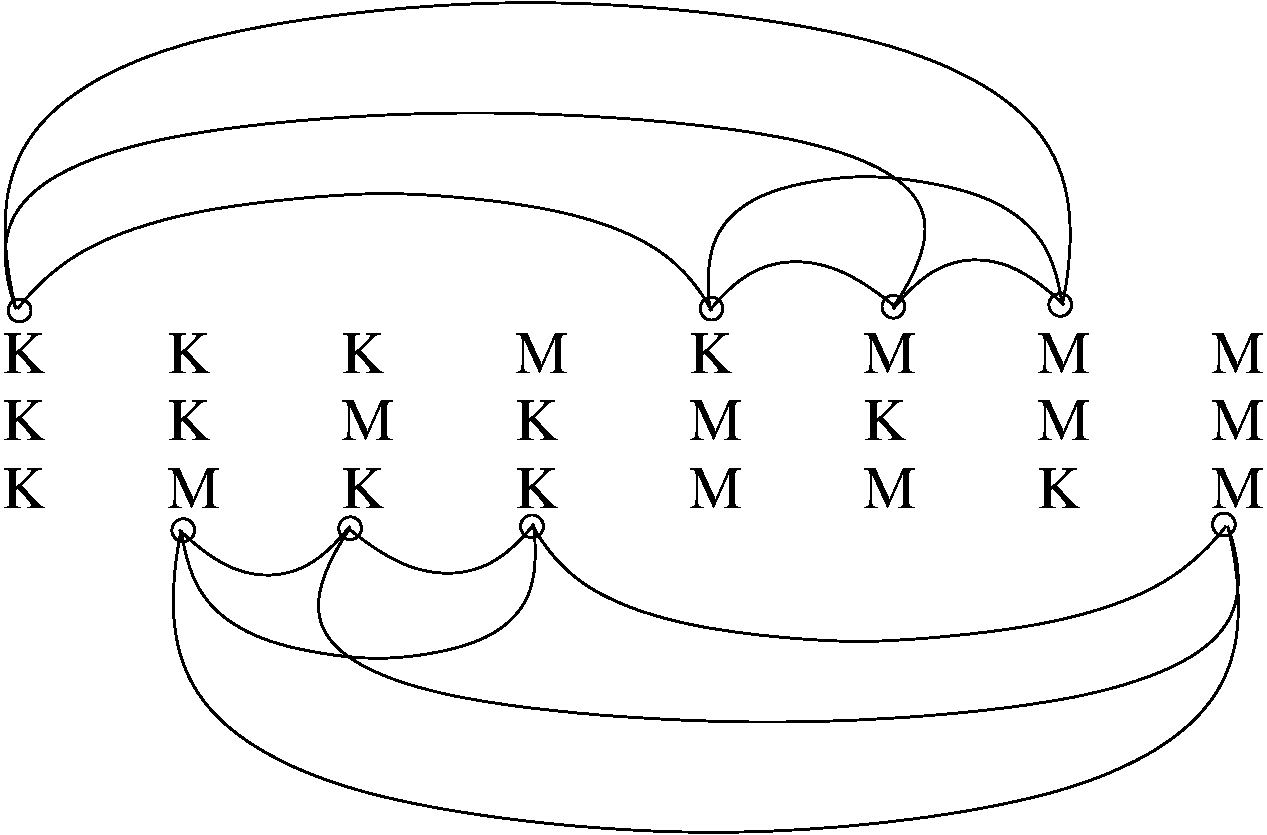
\includegraphics[width=0.5\linewidth,keepaspectratio]{munten}
\end{center}
\caption{De graaf met de 3 munten \label{munten}}
\end{figure}

Uit de graaf is vlug duidelijk dat het niet mogelijk is om van de KKK
configuratie tot MMM te komen terwijl de spelregels gerespecteerd
worden, omdat je niet van KKK naar MMM kan gaan door verbindingen te
volgen. KKK en MMM liggen in een verschillende component van de graaf.


\subsection{De wolf, de geit en de kool.}

Een boer bezit een wolf, een geit en een kool; hij leeft aan de
linkeroever van een rivier en wil al zijn bezittingen naar de overkant
brengen. Hij heeft een bootje, maar dat is niet groot genoeg om meer
dan \'{e}\'{e}n van zijn bezittingen tegelijk naar de overkant te
varen. Hij zou natuurlijk drie keer over kunnen varen met telkens
\'{e}\'{e}n van zijn bezittingen, maar zogauw hij de geit en de kool
alleen laat, eet de geit de kool op; en hetzelfde geldt voor de wolf
en de geit: dat wil de boer natuurlijk vermijden. Bestaat er een
manier om alles naar de overkant te brengen?

Om dit op te lossen, kan je natuurlijk alle mogelijkheden
proberen en dan zit je met het probleem van boekhouding. Hier is een
systematische manier om het te doen: schrijf eerst alle mogelijke
situaties neer; vermits een situatie volledig vastligt als je weet wat
op welke oever is, kan je dat doen door de voorstelling BGK te
gebruiken voor de situatie: de boer, de geit en de kool zijn op de
linkeroever. Sommige situaties zijn a priori verboden: GK zou willen
zeggen dat de geit en de kool op de linkeroever zitten (en de boer en
de wolf op de rechteroever of onderweg in het bootje) en dat is
verboden, want de geit zou de kool opeten. Alle situaties zijn dus
neer te schrijven als in Figuur~\ref{BWGK1}, waarbij $\ast$
gebruikt wordt om aan te duiden dat niets zich op de linkeroever
bevindt.

\begin{figure}[ht]
\mbox{
\hspace{1cm}
\subfigure[De mogelijke situaties voor de boer, de wolf, de geit en de kool ]{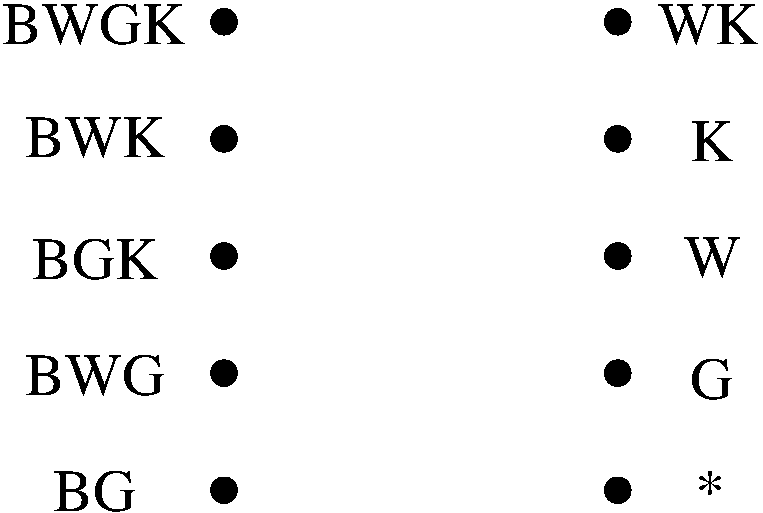
\includegraphics[height=0.12\textheight,keepaspectratio]{BWGK1} \label{BWGK1}}\hspace{2.5cm}
\subfigure[De graaf voor de wolf, de geit en de kool ]{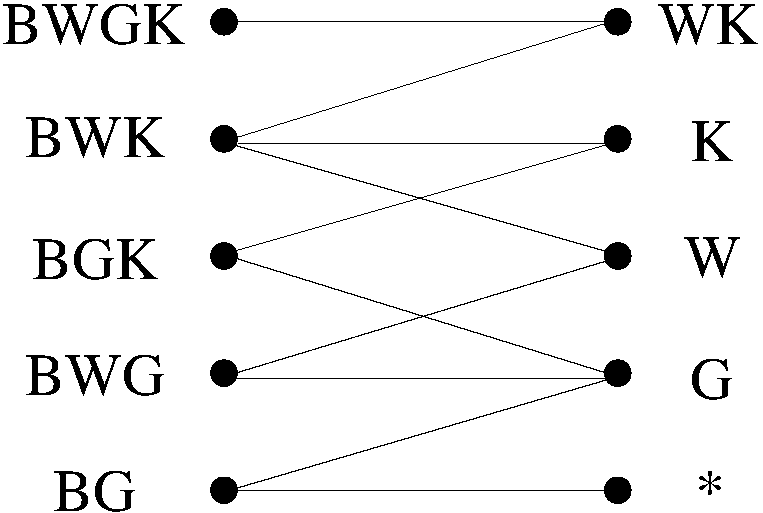
\includegraphics[height=0.12\textheight,keepaspectratio]{BWGK2} \label{BWGK2} }
}
\caption{De boer, de wolf, de geit en de kool}
\end{figure}

Vervolgens verbinden we elke twee situaties $\alpha$ en $\beta$ als de
boer door overvaren - en eventueel \'{e}\'{e}n van zijn bezittingen
mee te nemen - de situatie $\alpha$ in $\beta$ kan wijzigen. We
verkrijgen dan de graaf in Figuur~\ref{BWGK2}.  Het probleem is nu
herleid tot de vraag: bestaat er een pad langs de lijnen van de graaf
in Figuur~\ref{BWGK2} van punt BWGK naar $\ast$?

In het probleem van de munten en dat van de boer, wolf, geit en kool
hebben we telkens een probleem herleid tot de vraag naar het bestaan
van een pad tussen twee knopen in een graaf: dit is \'{e}\'{e}n van de
problemen in grafen die we zullen bestuderen. Dikwijls zijn we
ge\"{\i}nteresseerd in het kortste pad.

\subsection{De bruggen van K\"onigsberg}

18de eeuw, K\"onigsberg (nu Kaliningrad in Rusland): door de stad
stroomt de Pregel (Figuur~\ref{pregel}), een rivier met daarin twee
eilanden, onderling en met de oever verbonden door 7 bruggen. In het
weekend wandelen de inwoners van K\"onigsberg over de bruggen en vragen
zich af: is het mogelijk om een wandeling te maken die alle bruggen
\'{e}\'{e}n keer aandoet en zodat de wandeling begint en eindigt op
dezelfde plaats? In 1736 lost de Zwitser Leonhard Euler (1707-1783)
dit probleem op in het eerste artikel dat ooit over grafentheorie
verscheen.

\begin{figure}[ht]
\begin{center}
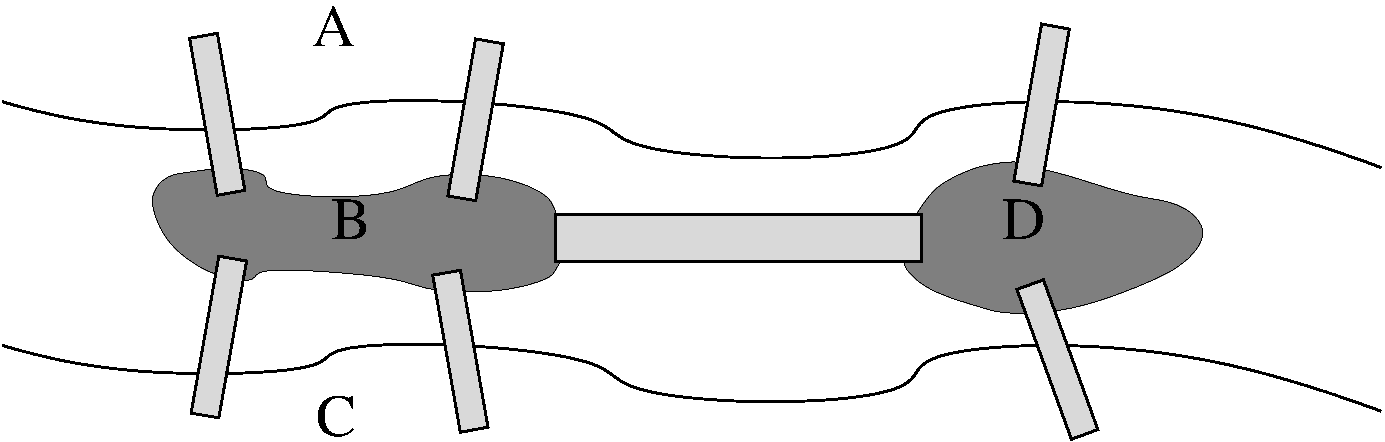
\includegraphics[width=0.4\linewidth,keepaspectratio]{pregel}
\end{center}
\caption{De bruggen aan de Pregelrivier \label{pregel}}
\end{figure}

Wat heeft het probleem met grafen te maken? Een voorstelling van de
bruggen en hoe ze oevers en eilanden verbinden m.h.v. een graaf vind
je in Figuur~\ref{pregelgraph}. Het probleem is nu teruggebracht tot
zijn essentie: bestaat in die graaf een kring, t.t.z. een gesloten
pad, dat alle bogen juist \'{e}\'{e}n maal aandoet? Zulk een kring
noemt men een Euleriaanse kring. Het zal blijken dat het
karakteriseren van grafen die een Euleriaanse kring hebben eenvoudig
is, alsook het vinden van een Euleriaanse kring.

\begin{figure}[ht]
\begin{center}
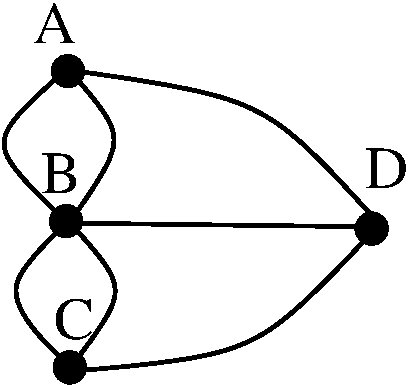
\includegraphics[width=0.15\linewidth,keepaspectratio]{pregelgraph}
\end{center}
\caption{De graaf die overeenkomt met de bruggen aan de Pregel
\label{pregelgraph}}
\end{figure}

Het zoeken van een Euleriaanse kring (of pad) ken je waarschijnlijk
ook van het volgende: gegeven een figuur waarin punten met lijnen
zijn verbonden, teken de figuur door je pen in een punt te
zetten, alle lijnen te volgen zonder een lijn twee keer te
doorlopen en zonder je pen ooit op te heffen.

In het {\em echte} leven is het vinden van een Euleriaanse kring ook
van belang, bijvoorbeeld als je de staat van de middenbermen van de
snelwegen in Belgi\"{e} wil controleren: je moet dan alle snelwegen
doorlopen maar je wil daarvoor liefst elke snelweg slechts \'{e}\'{e}n
keer afgaan.

\subsection{Het speelgoed van Hamilton}

Sir William Rowan Hamilton probeerde rond 1850 een
3-dimensionale puzzel op de markt te brengen in de vorm van een
dodecahedron (12 5-hoeken): Figuur~\ref{hamilton1} geeft een vlakke
weergave van die ruimtelijke figuur.  Elke hoek had de naam van een
stad en het probleem is van een weg te vinden die begint bij een stad,
elke stad juist \'{e}\'{e}n keer aandoet en terug bij de beginstad eindigt.
Zulk een weg wordt een Hamiltoniaanse kring genoemd: het zal heel
wat moeilijker blijken om het bestaan van een Hamiltoniaanse kring te
bewijzen of er \'{e}\'{e}n te construeren dan voor een Euleriaanse kring.

\begin{figure}[ht]
\begin{center}
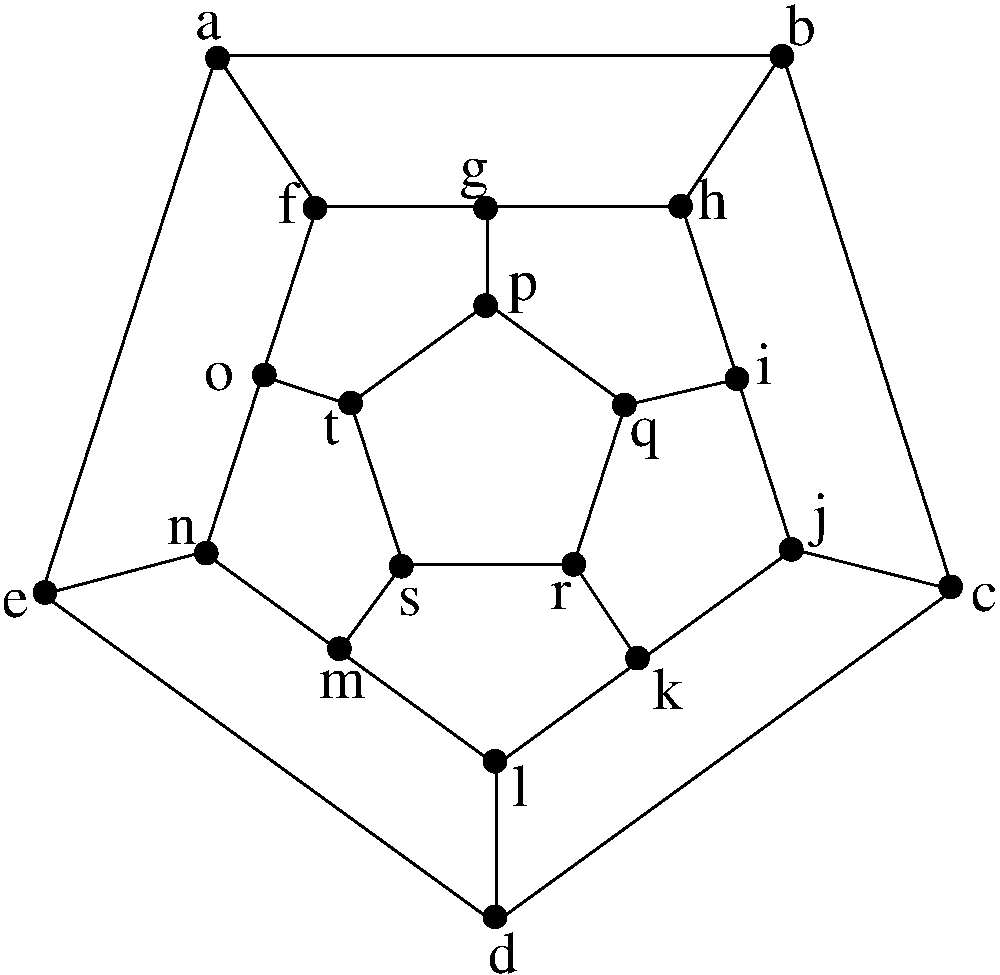
\includegraphics[width=0.4\linewidth,keepaspectratio]{hamilton}
\end{center}
\caption{De puzzel van Hamilton
\label{hamilton1}}
\end{figure}

De puzzel was een commerci\"{e}le flop, maar het is de voorloper van
het ``reizende verkopers-probleem'' (TSP) in een later hoofdstuk

Er is een probleem dat lijkt op het ``reizende verkopers-probleem'':
het postman-probleem; de postman wil op zijn ronde elke straat juist twee
maal doorlopen (eens langs elke kant van de straat) en de vraag is of
dat mogelijk is \ldots

Figuur~\ref{hamiltonkring} toont een Hamiltoniaanse kring voor de
puzzel van Hamilton.

\begin{figure}[ht]
\begin{center}
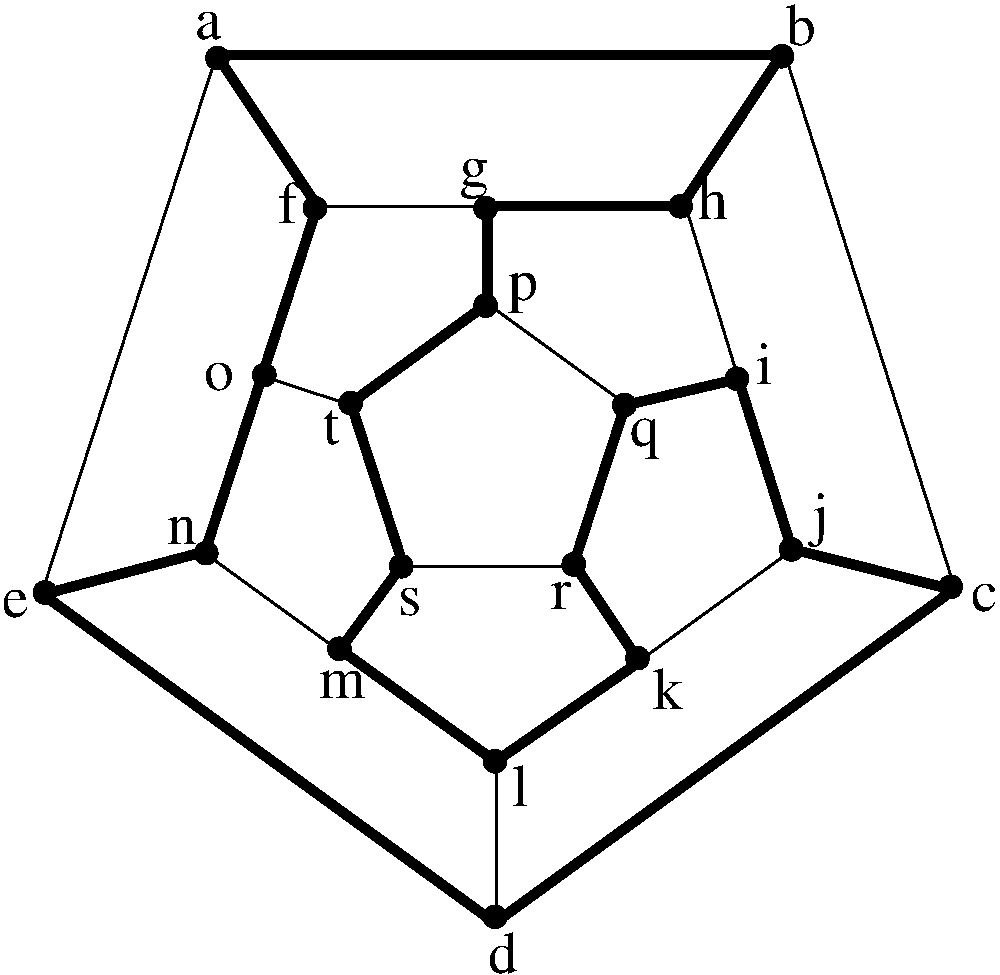
\includegraphics[width=0.6\linewidth,keepaspectratio]{hamiltonkring}
\end{center}
\caption{Een oplossing voor de puzzel van Hamilton
\label{hamiltonkring}}
\end{figure}

\clearpage
\section{Grafen}

\subsection{Allerhande paden}

\grijs{
\begin{definitie} Graaf\\
  \textup{ Een (niet-gerichte) \textbf{graaf} $G$ is een koppel $(V,E)$
    waarbij $V$ een verzameling van \textbf{knopen} (knoop = vertex) is
    en $E$ een
    (multi-)verzameling\footnotemark~
    van \textbf{bogen} (boog = edge)
    waarbij elke boog $e \in E$ een niet-geordend paar $(v,w)$ uit $V \times V$
    is; we schrijven $e = (v,w)$ of $e = (w,v)$. (In het Engels: (undirected) graph).}
\end{definitie}
}
\footnotetext{Het begrip $multiverzameling$ is  analoog aan dat van een 
verzameling, met die uitzondering dat een element meer dan eens mag 
voorkomen, bv.\ $\{1,1,1,2,2,3,4,5,5\}$ is een multiverzameling.}

We staan ons soms wat vrijheid van notatie toe:
\begin{itemize}
\item
we schrijven $G(V,E)$ als afkorting voor: de graaf $G$ met knopen $V$ en bogen $E$
\item
we schrijven $e \in G$ voor: $e \in E$ waarbij $E$ de bogen van $G$ zijn (als we al
weten dat $e$ een boog is)
\item
we schrijven $v \in G$ voor: $v \in V$ waarbij $V$ de knopen van $G$ zijn (als we al
weten dat $v$ een knoop is)
\item
als $e$ een boog is met eindknopen $x,y$ en $G$ de graaf $(V,E)$, dan
bedoelen we met $G \cup \{e\}$ de graaf $(V \cup \{x,y\},E \cup \{e\})$:
we zeggen ``voeg $e$ toe aan $G$''
\item
als $b$ een knoop is en $G$ de graaf $(V,E)$, dan bedoelen we met $G
\cup \{b\}$ de graaf $(V \cup \{b\},E )$ en we zeggen ``voeg $b$ toe
aan $G$''
\end{itemize}

Soms veronderstellen we impliciet dat de knopen genummerd zijn van 1
tot $n$ met $n$ het aantal knopen. We zullen ook enkel met eindige
grafen te maken hebben.



Een boog wordt ook soms een ribbe genoemd en een knoop een top: dit
naar analogie met veelvlakken die mee aan de oorsprong liggen van de
grafentheorie.


Merk op dat in $E$ twee bogen $(v,w)$ kunnen voorkomen: we noemen zulke
bogen \textbf{parallel}.

We zeggen dat de boog $(v,w)$ invalt (``is incident on'') in de knoop $v$ (en
$w$) en dat de knopen $v$ en $w$ grenzen (``are adjacent to'') aan de boog
$(v,w)$.

\grijs{
\begin{definitie} Gerichte graaf\\
  \textup{ Een \textbf{gerichte graaf} G is een paar $ (V,E)$ waarbij $V$
    een verzameling van knopen is en $E$ een (multi-)verzameling van
    bogen waarbij elke boog $e \in E$ een geordend paar $(v,w)$ uit
    $V\times V$ is; we schrijven $e = (v,w)$. (in het Engels: directed graph of digraph)}
\end{definitie}
}


\grijs{
\begin{definitie} Lus\\
  \textup{Een \textbf{lus} in een graaf is een boog $(v,v)$. }
\end{definitie}
}


\grijs{
\begin{definitie} Enkelvoudige graaf\\
\textup{Een graaf is \textbf{enkelvoudig} als de graaf geen parallelle bogen
noch lussen heeft. }
\end{definitie}
}


\grijs{\begin{definitie} Graad van een knoop\\
  \textup{De \textbf{graad $\delta(v)$ van een knoop $v$} van de graaf
    $(V,E)$ is het aantal bogen $(v,w) \in E$.}
\end{definitie}}

{\bf Opmerking:} Een lus in een knoop $v$ draagt een factor 2 bij tot de 
graad $\delta(v)$. 

\grijs{\begin{definitie} Ge\"{\i}soleerde knoop\\
Een knoop $v$ in een graaf $(V,E)$ noemt men {\bf ge\"{\i}soleerd} indien 
$\delta(v)=0$.
\end{definitie}}


\grijs{\begin{stelling} \label{somgraad} Som van de graden van de knopen\\
De som van de graden van de knopen van een graaf is even.
\end{stelling}}
\begin{proof}
Vermits elke boog $(v,w)$ \'{e}\'{e}n bijdraagt tot de graad van zowel $v$
als $w$, is de bijdrage van elke boog tot de som van de graden gelijk
aan twee en bijgevolg is de som van de graden van de knopen van een graaf
even.
\end{proof}


\grijs{\begin{stelling} Aantal knopen met oneven graad\\
In elke graaf is er een even aantal knopen met oneven graad.
\end{stelling}}
\begin{proof}
Als de graaf knopen $a_i$ ($i=1,\ldots,n$) heeft met even graad en $b_i$ ($i=1,\ldots,m$)
met oneven graad, dan is door Stelling~\ref{somgraad}
\[0 = \left(\sum_{i=1}^{n} \delta(a_{i}) + \sum_{i=1}^{m} \delta(b_{i})\right)
\bmod 2 = m \bmod 2 \] en bijgevolg is de stelling waar.  \end{proof}


\grijs{\begin{definitie} Pad\\
\textup{Een \textbf{pad} (van lengte $n$) in een graaf $(V,E)$ is een
 rij bogen
\[( e_1=(v_{1},v_{2}),\;e_2=(v_{2},v_{3}),\;\ldots, e_{n}=(v_{n},v_{n+1})).\]\\
Impliciet wordt hier verondersteld dat bij het geven van een pad, het
duidelijk is welke van de (eventueel) parallelle bogen in het pad
gebruikt worden.\\
Anderzijds is in een enkelvoudige graaf, een pad ook gekarakteriseerd
door de rij knopen $(v_{1}, \ldots , v_{n+1})$, maar in een graaf die niet
enkelvoudig is, kan zulk een rij knopen staan voor meerdere paden.}
\end{definitie}}


\grijs{\begin{definitie} Enkelvoudig pad\\
  \textup{Een \textbf{enkelvoudig pad} $(v_{1}, \ldots , v_{n+1})$ is een pad
  waarvan voor alle $i \neq j$ geldt dat $v_{i} \neq v_{j}$ }
\end{definitie}}



\grijs{\begin{definitie} Kring\\
  \textup{Een \textbf{kring} is een pad
    $((v_1,v_2),...,(v_n,v_{n+1}))$, waarbij alle gebruikte bogen
    onderling verschillend zijn en waarbij $v_{1} = v_{n+1}$.}
\end{definitie}}

Een kring wordt ook een circuit genoemd.


\grijs{\begin{definitie} Euleriaanse kring (pad)\\
  \textup{Een \textbf{Euleriaanse kring (pad)} is een kring (pad) die
  alle bogen van een graaf juist \'e\'en maal aandoet en ook alle knopen
  doorloopt.}
\end{definitie}}


\grijs{\begin{definitie} Hamiltoniaanse kring\\
  \textup{ Een \textbf{Hamiltoniaanse kring} is een kring die
  alle knopen van een graaf juist \'{e}\'{e}n  keer aandoet.}
\end{definitie}}


\grijs{\begin{definitie} Samenhangende graaf\\
  \textup{ Een graaf is \textbf{samenhangend} als er voor elke twee
    verschillende knopen $v$ en $w$ een pad is van $v$ naar $w$.}
\end{definitie}}



\grijs{\begin{stelling} Het bestaan van een Euleriaanse kring.\\
  Een graaf $G(V,E)$ heeft een Euleriaanse kring als en slechts als $G$
  samenhangend is en de graad van elke knoop even is.
\end{stelling}}
De intu\"{\i}tie achter het bewijs is dat wanneer je in een knoop toekomt, je er
nog altijd weg kan geraken, vermits de graad even is: daardoor maakt
het niet zo veel uit welk pad je volgt als je maar niet te vlug
terugkeert naar je startpunt. Deed je dat wel, dan kan het pad nog
aangepast worden.



\begin{proof}
\begin{itemize}
\item Indien de graaf een Euleriaanse kring heeft dan is de graaf
  samenhangend, want de kring verbindt alle knopen en er is dus een
  pad van elke knoop naar elke andere knoop. Vermits bij het doorlopen
  van een kring, we telkens ook vertrekken uit een knoop waar we
  toekwamen, en vermits alle bogen doorlopen worden door een
  Euleriaanse kring, moet de graad van elke knoop even zijn.
\item Construeer een kring $P$ in de graaf als volgt: start bij een
  willekeurige knoop $s$, volg een willekeurige boog die invalt in $s$; vanaf
  dan, breid het partieel pad uit met een willekeurige boog vanaf de
  laatst toegevoegde knoop, maar gebruik geen boog meer dan eens.
  Herhaal totdat er geen boog meer voorhanden is. Vermits elke knoop
  een even graad
  heeft, is $P$ een kring die in $s$ vertrekt en aankomt. 
  Indien $P$ alle bogen van $G$ gebruikt, is de stelling 
  bewezen. In het andere geval is er een knoop $s'$ op het pad $P$, waaruit 
  er eveneens een boog vertrekt die niet tot $P$ behoort (waarom?). 
  Construeer nu in $s'$ een kring $P'$ die geen bogen van $P$ gebruikt (waarom 
  kan dit?). We kunnen $P'$ toevoegen aan $P$ om een kring te bekomen, die
  meer bogen gebruikt dan $P$. We kunnen deze procedure herhalen totdat er 
  geen ongebruikte bogen meer zijn:  de Euleriaanse kring is geconstrueerd.
  Figuur~\ref{euler4} illustreert de
  constructie.
\end{itemize}
\begin{figure}[ht]
\begin{center}
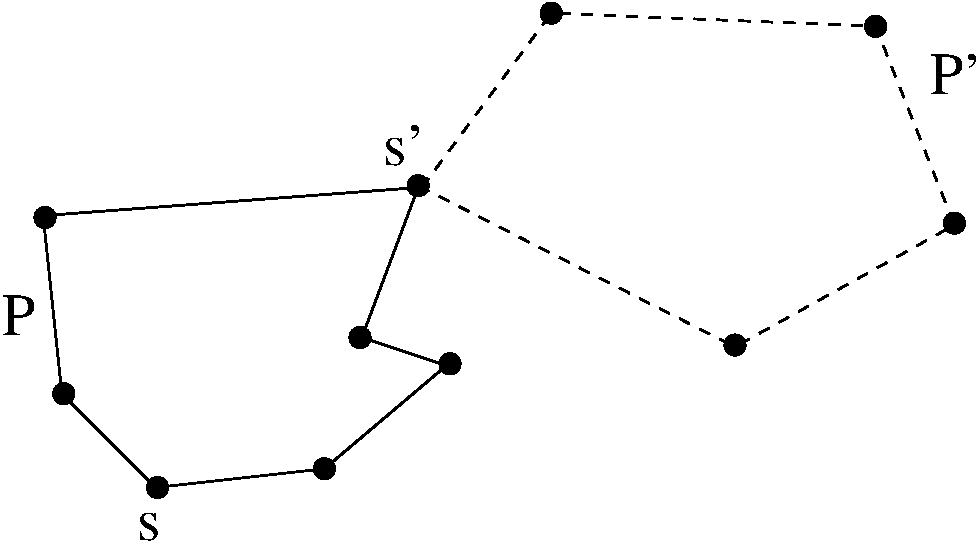
\includegraphics[width=0.4\linewidth,keepaspectratio]{euler4}
\end{center}
\caption{ $P$ en de uitbreiding $P'$ \label{euler4}}
\end{figure}
\end{proof}


\grijs{\begin{stelling} Bestaan van een Euleriaans pad\\
  Een samenhangende graaf $G$ heeft een Euleriaans pad van knoop $v$ naar $w$
  ($v \neq w$) indien $v$ en $w$ de enige knopen zijn met oneven graad.
\end{stelling}}
\begin{proof} Beschouw de graaf $G'$ die je verkrijgt door aan $G$ de
boog $(w,v)$ toe te voegen. $G'$ is samenhangend en elke knoop heeft nu
een even graad, bijgevolg bestaat een Euleriaanse kring $(w,v,\ldots,w)$;
laat uit die kring de eerste boog weg en je verkrijgt een pad
$(v,\ldots,w)$ in $G$.
\end{proof}

Als je nu terugkijkt naar Figuur~\ref{pregelgraph} (de graaf voor de bruggen in K\"onigsberg), dan zie je dat
alle vier de knopen een oneven graad hebben en dus niet voldoen aan de
voorwaarden van de stellingen van Euler; bijgevolg is er geen
Euleriaanse kring (noch Euleriaans pad) in die graaf en dus heeft het
probleem van de bruggen aan de Pregel een negatieve oplossing.



\grijs{\begin{definitie} Deelgraaf\\
  \textup{Een graaf $(V_1,E_1)$ is een \textbf{deelgraaf} van $(V,E)$ indien
    $V_1 \subseteq V$ en $E_1 \subseteq E$.}
\end{definitie}}



 \grijs{\begin{definitie} Component van een graaf\\
  \textup{Een \textbf{component} $C$ van een graaf $G$ is een maximaal
    samenhangende deelgraaf van $G$, t.t.z.
$\forall C' \subseteq G: C \subset C' \Rightarrow C'$ is niet samenhangend.}
\end{definitie}}

 \grijs{\begin{stelling} \label{partitie} Partitie van een graaf\\
De componenten $(V_{i},E_{i})$ ($i=1,\ldots,n$) van een graaf $(V,E)$ 
vormen een partitie,
t.t.z. \\
$(V,E) = (\cup_{i=1}^{n} V_{i},\cup_{i=1}^{n} E_{i})$ en
voor $i \neq j$, $V_{i} \cap V_{j} = \emptyset$ en $E_{i} \cap E_{j} =
\emptyset$
\end{stelling}}
\begin{proof} Het is duidelijk dat elke knoop tot minstens
\'{e}\'{e}n component moet behoren en ook elke boog. Stel dat een
knoop tot twee componenten $\alpha$ en $\beta$ behoort, dan is de unie
van $\alpha$ en $\beta$ een samenhangende deelgraaf van $(V,E)$ en
bijgevolg moet $\alpha = \beta$ en daaruit volgt dat $V_{i} \cap V_{j}
= \emptyset$ voor $i \neq j$. Vermits een boog behoort tot de
component van zijn eindknopen, is het bewijs gemakkelijk te vervolledigen.
\end{proof}


De Stelling~\ref{partitie} is belangrijk omdat het dikwijls
eenvoudiger is eigenschappen te bewijzen voor samenhangende grafen en
Stelling~\ref{partitie} geeft ons een manier om op eenduidige wijze
een niet-samenhangende graaf in samenhangende delen te verdelen.



\subsection{Voorstelling van grafen \label{voorstelgraaf}}

Tot nog toe hebben we grafen gewoon getekend. Dikwijls hebben we ook
een meer formele voorstelling van grafen nodig, bijvoorbeeld als we
programma's schrijven die grafen behandelen. Sommige voorstellingen
lenen zich beter tot manipulatie dan andere en we zullen dan ook
meerdere voorstellingsmanieren bekijken. We bekijken eerst
niet-gerichte grafen en daarna gebruiken we een variante om gerichte
grafen voor te stellen.

Voor een graaf $G(V,E)$ met $n$ knopen kunnen we de knopen nummeren van 1
tot $n$ en een $n\times n$ matrix opstellen met op de $(i,j)$-de plaats 
een 1 als
$(i,j) \in E$ en anders een 0; die matrix noemen we de
buurmatrix van $G$.

\begin{figure}[ht]
\begin{center}
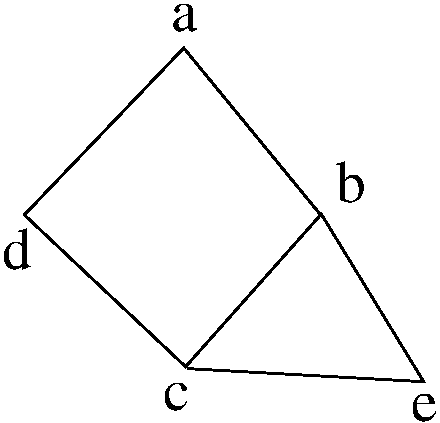
\includegraphics[width=0.2\linewidth,keepaspectratio]{adjacency1}
\end{center}
\caption{ Voorbeeld \label{adjacency1}}
\end{figure}

De buurmatrix $A$ van de graaf van Figuur~\ref{adjacency1} is

\begin{center}
\mbox{\space \space \space}
$\begin{array}{ccccc}
a & b & c & d & e\\
\end{array}
$\\
$
\begin{array}{c}
a\\
b\\
c\\
d\\
e\\
\end{array}
$
$
\left(
\begin{array}{ccccc}
0 & 1 & 0 & 1 & 0\\
1 & 0 & 1 & 0 & 1\\
0 & 1 & 0 & 1 & 1\\
1 & 0 & 1 & 0 & 0\\
0 & 1 & 1 & 0 & 0\\
\end{array}
\right)
$
\end{center}

Een buurmatrix van een enkelvoudige graaf heeft op de
diagonaal alleen maar nullen. Aan de buurmatrix van een graaf kan je niet zien of
de graaf parallelle bogen heeft of niet. Een buurmatrix is
steeds symmetrisch en daarom niet erg effici\"ent als voorstelling. Toch
heeft de buurmatrix interessante eigenschappen.

Laat ons $A^{2}$ berekenen; we verkrijgen:

\begin{center}
$
A^{2} = \left(
\begin{array}{ccccc}
2 & 0 & 2 & 0 & 1\\
0 & 3 & 1 & 2 & 1\\
2 & 1 & 3 & 0 & 1\\
0 & 2 & 0 & 2 & 1\\
1 & 1 & 1 & 1 & 2\\
\end{array}
\right)
$
\end{center}

We verkregen het $(a,c)$-de element van $A^{2}$ door:

\begin{center}
$
\left(
\begin{array}{ccccc}
0 & 1 & 0 & 1 & 0\\
\end{array}
\right)
\times
\left(
\begin{array}{c}
0\\
1\\
0\\
1\\
1\\
\end{array}
\right)
 =
0\times 0 + 1\times 1 + 0\times 0 + 1\times 1 + 0\times 1 = 2$
\end{center}

en de positieve bijdragen aan het resultaat komt van paden $(a,b)-(b,c)$
en $(a,d)-(d,c)$. Dat wijst erop dat $A^{2}[i,j] = $ het aantal paden
van knoop $i$ naar knoop $j$ met lengte 2. Maar we moeten toch
oppassen met die uitspraak: de buurmatrix laat geen parallelle bogen
zien en parallelle bogen vergroten het aantal paden tussen twee knopen.
Daarom beperkt de volgende stelling zich tot enkelvoudige grafen:

 \grijs{\begin{stelling}
\label{aantalpaden}
$ $ \\
% om niet buiten de kantlijn te gaan.
Indien $A$ de buurmatrix is van een enkelvoudige graaf $G(V,E)$,\\
dan is
$A^{n}[i,j] = $ het aantal paden met lengte $n$ van knoop $i$ naar knoop
$j$.
\end{stelling}}
\begin{proof} We gebruiken inductie op $n$. Voor $n=1$ is de
stelling waar door de definitie van buurmatrix.

Stel dat de stelling waar is voor $n$, we bewijzen dat de stelling waar
is voor (n+1): we weten dat $A^{n+1}=A^{n}*A$ en dus $A^{n+1}[i,j] =
\sum_{k=1}^{\#V} A^{n}[i,k]*A[k,j]$; door de inductiehypothese is
$A^{n}[i,k]$ het aantal paden van $i$ naar $k$ en als er een boog van $k$
naar $j$ is (t.t.z. als $A[k,j] = 1$) dan zijn er ook $A^{n}[i,k]$
aantal paden van $i$ naar $j$ die langs $k$ passeren juist voor ze in $j$
toekomen. Vermits geen twee paden dezelfde zijn (waarom niet?)
verkrijgen we het resultaat voor $(n+1)$.
\end{proof}

Voor de graaf van Figuur~\ref{adjacency1} is
\begin{center}
$A^{4} = \left(
\begin{array}{ccccc}
9 & 3 & 11& 1 & 6\\
3 & 15& 7 & 11& 8\\
11& 7 & 15& 3 & 8\\
1 & 11& 3 & 9 & 6\\
6 & 8 & 8 & 6 & 8\\
\end{array}
\right)
$
\end{center}

Gebruik makend van voorgaand resultaat kunnen we inzien dat
$(\sum_{k=1}^{n} A^{k})[i,j]$ gelijk is aan het aantal paden korter
dan $n$ bogen van $i$ naar $j$.

Een ander gebruik van de buurmatrix vinden we door de buurmatrix niet
te vullen met 0 of 1, maar met met de boolse waarden $true$ of $false$;
matrixvermenigvuldiging wordt dan gedefinieerd als:

\[(A*B)[i,j] = (A[i,1] \wedge B[1,j]) \vee (A[i,2] \wedge B[2,j]) \vee
\ldots \vee (A[i,n] \wedge B[n,j])\]


Als $B$ de boolse buurmatrix van de graaf $G$ voorstelt, dan is
$B^{n}[i,j]$ gelijk aan de waarheidswaarde van ``er is een pad met
lengte $n$ van $i$ naar $j$''.

En analoog is $(\sum_{k=1}^{n} B^{k})[i,j]$ (de som is hier ook nu de boolse
som, t.t.z. $\vee$) de waarheidswaarde van ``er is een pad
van lengte kleiner dan of gelijk aan $n$ van $i$ naar $j$''. 
Terwijl
de waarden in de machten van de gewone buurmatrix onbeperkt
stijgen, zijn die voor de boolse buurmatrix $false$ of $true$ en
monotoon stijgend en dus bestaat
de limiet.
Het is een manier om de
transitieve sluiting van de relatie gedefinieerd door de bogen te
berekenen en
de limiet
wordt gevonden na hoogstens $n$
vermenigvuldigingen, als $n$ het aantal knopen in de graaf is. We zien
hiervan een toepassing bij gerichte grafen.

Een andere voorstelling van een graaf is gegeven door de incidentiematrix 
$I$: die heeft voor elke knoop een rij en voor elke boog een
kolom. $I[i,j] = 1$ indien de $j$-de boog $i$ als eindpunt heeft en anders 0.
De incidentiematrix van de graaf in Figuur~\ref{adjacency1}
% \newpage

\begin{center}
\mbox{\space \space \space}
$\begin{array}{cccccc}
ab & ad & cd & bc & ce & be\\
\end{array}
$\\
$
\begin{array}{c}
a\\
b\\
c\\
d\\
e\\
\end{array}
$
$
\left(
\begin{array}{cccccc}
1 & \hspace{0.18cm} 1 & \hspace{0.18cm}0 & \hspace{0.18cm}0 & \hspace{0.18cm}0 & \hspace{0.18cm}0\\
1 & \hspace{0.18cm}0 & \hspace{0.18cm}0 & \hspace{0.18cm}1 & \hspace{0.18cm}0 & \hspace{0.18cm}1\\
0 & \hspace{0.18cm}0 & \hspace{0.18cm}1 & \hspace{0.18cm}1 & \hspace{0.18cm}1 & \hspace{0.18cm}0\\
0 & \hspace{0.18cm}1 & \hspace{0.18cm}1 & \hspace{0.18cm}0 & \hspace{0.18cm}0 & \hspace{0.18cm}0\\
0 & \hspace{0.18cm}0 & \hspace{0.18cm}0 & \hspace{0.18cm}0 & \hspace{0.18cm}1 & \hspace{0.18cm}1\\
\end{array}
\right)
$
\end{center}

In de incidentiematrix vind je lussen en ook parallelle bogen terug.



De voorstelling van een gerichte graaf kan gebeuren zoals bij
niet-gerichte grafen: een buurmatrix die een 1 heeft op de $(i,j)$-de
plaats indien er een gerichte boog van $i$ naar $j$ bestaat, en anders
een 0. De matrix is nu niet meer symmetrisch, maar we hebben daar
eigenlijk nooit gebruik van gemaakt en de veralgemening van stelling
\ref{aantalpaden} ligt voor de hand, evenals de definitie van de
boolse buurmatrix.



Een belangrijke toepassing van de boolse buurmatrix ligt in het
opsporen van de functies die opgeroepen worden (rechtsreeks of
onrechtsreeks) door een andere functie in het programma; de
directe-oproep relatie kan men voorstellen door een gerichte graaf of
door zijn boolse buurmatrix $B$. De matrix verkregen als de boolse som
$\sum B^{i}$ stelt de transitieve sluiting van de boog-relatie voor en
bevat rechtstreeks de informatie of een functie een andere oproept of
niet. Het is bovendien gemakkelijk te zien welke functies nooit
opgeroepen worden: dat zijn de functies die niet verbonden zijn met de
hoofdfunctie (main);
zulke functies zijn in het compiler jargon {\em dode code}. In
sectie~\myref{sccs} gebruiken we dit voorbeeld nog eens voor een
interessant grafenalgoritme.

\subsection{Isomorfisme van grafen}

We voeren het volgende experiment uit: een groep studenten wordt
gevraagd een blad en een pen te nemen en zonder spieken de opdracht
uit te voeren

\begin{itemize}
\item[]
- teken 5 punten en zet er een naam bij \\
- verbind het eerste punt dat je tekende met het tweede\\
- verbind het tweede met het derde punt\\
- verbind het derde met het vierde\\
- verbind het vierde met het vijfde\\
- verbind het vijfde met het eerste\\
\end{itemize}

Er is een goede kans dat sommige studenten \'{e}\'{e}n van de grafen
uit Figuur~\ref{experiment1} hebben getekend.

\begin{figure}[ht]
\begin{center}
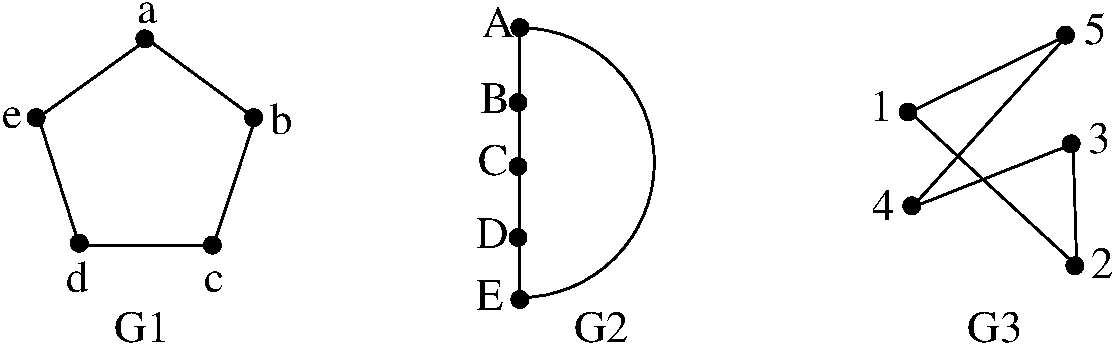
\includegraphics[width=0.6\linewidth,keepaspectratio]{experiment1}
\end{center}
\caption{Drie verschillende of drie dezelfde grafen?\label{experiment1}}
\end{figure}

Al zien die grafen er verschillend uit, ze zijn getekend aan de hand
van dezelfde instructies en we zouden ze dus graag als gelijk
beschouwen, daarom de volgende definitie:

 \grijs{\begin{definitie} \label{isomorfegrafen} Isomorfisme van grafen\\
\textup{De grafen $G_{i}(V_{i},E_{i})$ (i = 1,2) worden
    \textbf{isomorf} genoemd, indien er een bijectie $f: V_{1}
    \rightarrow V_{2}$ bestaat zodanig dat $g: E_{1} \rightarrow E_{2}$
    gedefinieerd door $g((v,w)) = (f(v),f(w))$ voor
    alle $v,w \in E_{1}$ goed gedefinieerd (d.w.z. dat $g((v,w)) \in E_{2}$) is en een bijectie.
    Dergelijke $f$ noemen we een isomorfisme tussen de twee grafen.}
\end{definitie}}

Tussen graaf $G_{1}$ en $G_{2}$ van Figuur~\ref{experiment1} kan een
isomorfisme $f$ gedefinieerd worden door:
\begin{itemize}
\item[]
f(a) = B\\
f(b) = C\\
f(c) = D\\
f(d) = E\\
f(e) = A
\end{itemize}

en je kan nagaan dat $G_{1}$ en $G_{2}$ inderdaad isomorf zijn. Er is
een andere karakterisatie van isomorfe grafen m.b.v. de volgende stelling:

 \grijs{\begin{stelling} Karakterisatie van isomorfe grafen m.b.v. de incidentiematrix\\
  De grafen $G_{1}$ en $G_{2}$ zijn isomorf als en slechts als er een ordening van
  de knopen en bogen bestaat waarvoor de incidentiematrices van
  $G_{1}$ en $G_{2}$ gelijk zijn.
\end{stelling}}
\begin{proof}
\begin{itemize}
\item 
Veronderstel dat $G_{1}$ en $G_{2}$ isomorf zijn, via een isomorfisme $f$.
Kies een willekeurige orde op de knopen
  van $G_{1}$, dan volgt de orde op de knopen van $G_{2}$ door: $f(v)
  < f(w)$ $\Leftrightarrow v < w$; de orde op de bogen van $G_{2}$
  wordt analoog ge\"{\i}nduceerd door 
de orde op de bogen
van $G_{1}$ en 
  de bijectie tussen de bogen. De incidentiematrices zullen gelijk
  zijn.
\item Als de incidentiematrices gelijk zijn, is het isomorfisme $f$
  triviaal te construeren en 
het isomorf zijn
volgt direct.
\end{itemize}
\end{proof}

We weten al dat de buurmatrix niet volledig een graaf bepaalt: immers
parallelle bogen zijn niet zichtbaar in de buurmatrix. Daarom de meer
beperkte stelling:

 \grijs{\begin{stelling} Karakterisatie van isomorfe enkelvoudige grafen m.b.v. de buurmatrix\\
  De enkelvoudige grafen $G_{1}$ en $G_{2}$ zijn isomorf als en slechts als er een
  ordening van de knopen bestaat waarvoor de buurmatrices van
  $G_{1}$ en $G_{2}$ gelijk zijn.
\end{stelling}}
\begin{proof} Het bewijs mag je zelf geven.
\end{proof}



De stellingen over isomorfisme van grafen, geven een manier om
isomorfisme te testen bij een meer concrete voorstelling van de graaf
(m.b.v. de buur- of incidentiematrix): dat is nuttig bij het programmeren.


Elk bekend algoritme om te testen of twee grafen isomorf zijn, is
minstens exponentieel. Er bestaan echter heel effici\"ente testen die
kunnen aantonen dat twee grafen {\em niet} isomorf zijn: daarbij gaat
men na of een eigenschap die invariant is onder isomorfisme, geldig is
voor beide grafen. De eenvoudigste voorbeelden van invariante
eigenschappen (onder isomorfisme van grafen) is ``het aantal knopen''
en ``het aantal bogen'': dat volgt direct uit definitie
\ref{isomorfegrafen}. Wanneer we meer over grafen hebben geleerd,
zullen we nog meer eenvoudig te testen eigenschappen kennen die al dan
niet invariant zijn onder isomorfisme.



\subsection{Gewogen grafen}

 \grijs{\begin{definitie} Gewogen graaf\\
  \textup{ Een \textbf{gewogen graaf} $(V,E)$ is een graaf waarbij
    elke boog $e \in E$ een \textbf{gewicht $w(e)$} 
    $\in \R^{+}_0$
    heeft.
    Het gewicht $w(G)$ van een gewogen graaf $G$, is de
    som van de gewichten van de bogen van $G$.
}
\end{definitie}}


Het gewicht van een boog kan men zien als de lengte van de boog of een
kost geassocieerd met het doorlopen van de boog: de graaf kan
bijvoorbeeld een wegennetwerk tussen steden voorstellen en het gewicht
is dan de afstand tussen steden of de tol die voor het gebruik van de
weg tussen twee steden geheven wordt. Met het \textbf{gewicht van een
graaf} bedoelt men de som van de gewichten van alle bogen van de
graaf; met \textbf{gewicht van een pad} de som van de gewichten van de
bogen van het pad. Als de graaf een wegennetwerk voorstelt, is het
duidelijk dat het kennen van een \textbf{kortste pad} tussen twee
knopen, t.t.z. een pad met kleinste gewicht dat de twee knopen
verbindt, interessant is. Vermits deze twee knopen noodzakelijkerwijze
in dezelfde component moeten liggen (waarom?) hebben we het in deze
sectie steeds over samenhangende grafen.

Het bestaan van een kortste pad in een samenhangende (eindige!)  graaf
ligt voor de hand, en werd uitvoerig behandeld in andere vakken.

We zullen in deze sectie steeds met enkelvoudige grafen werken:
immers, lussen komen niet voor in een kortste pad en van een stel
parallelle bogen hebben we genoeg met de kortste. (je kan dat zelf
formeel bewijzen).

Algoritmen in dit hoofdstuk bestaan uit een opeenvolging van
opdrachten genummerd 1,2, \ldots . Op het textueel einde van elke
opdracht $n$ staat impliciet 
{\bf Ga naar opdracht (n+1)}.
Met ``stop'' wordt bedoeld dat het algoritme gedaan is.


\subsection{Vlakke grafen}

Intu\"{i}tief is een vlakke graaf, een graaf die je op papier kan
tekenen zonder dat twee bogen mekaar snijden: je hebt geen derde
dimensie nodig om de graaf te realiseren. Bij de studie van vlakke
grafen, spelen bepaalde grafen met een speciale eigenschap een belangrijke rol:
de grafen waarvan de knopen in twee disjuncte verzamelingen kunnen
verdeeld worden zodanig dat er geen bogen zijn tussen knopen binnen
dezelfde verzameling. Figuur~\ref{kuratowski1} laat zulk een graaf
zien.

 \grijs{\begin{definitie} Tweeledige graaf\\
  \textup{Een \textbf{tweeledige graaf} is een graaf $(V,E)$ waarvan $V =
    V_{1} \cup V_{2}$ zodanig dat $V_{1} \cap V_{2} = \emptyset$ en
    $E \subseteq V_{1} \times V_{2}$ }
\end{definitie}}


Met $K_{n,m}$ zullen we in het vervolg de tweeledige graaf aanduiden
waarvan $V_{1}$ $n$ elementen bevat en $V_{2}$ $m$ en waarvan elke knoop
van $V_{1}$ verbonden is met elke knoop van $V_{2}$. $K_{n,m}$ komt
van pas als je $n$ huizen wil verbinden met $m$ nutsvoorzieningen (water,
elektriciteit, gas, internetaansluiting \ldots).

Met $K_{n}$ zullen we de graaf met $n$ knopen aanduiden, waarbij er
een boog is tussen elke twee knopen - zulke grafen noemt men
\textup{volledig verbonden} en met spreekt ook wel van een kliek (in
het Engels clique).

De $K$ is ter ere van Kazimierz Kuratowski.

In Figuur~\ref{kuratowski1} vind je een voorstelling van $K_{4}$ en
van $K_{2,2}$.

\begin{figure}[ht]
\begin{center}
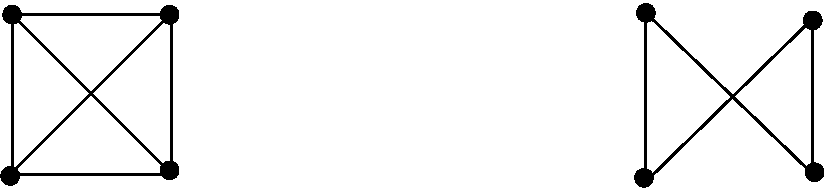
\includegraphics[width=0.4\linewidth,keepaspectratio]{kuratowski1}
\end{center}
\caption{$K_{4}$ en $K_{2,2}$ \label{kuratowski1}}
\end{figure}

Als je $K_{n}$ tekent op papier voor opeenvolgende waarden van $n$, en
je probeert dat te doen zodanig dat geen twee bogen mekaar kruisen op
je tekening, dan merk je dat je vanaf $n=5$ daar niet meer in
slaagt. En als je $K_{n,m}$ tekent voor opeenvolgende waarden van
$(n,m)$ merk je dat de graaf steeds kruisende bogen heeft voor 
$n,m > 2$.

Er is iets speciaals aan grafen die je kan tekenen zonder dat bogen
mekaar kruisen: zulke grafen worden \textbf{vlak} genoemd. Een
toepassing van het begrip {\em vlakke graaf} vind je in het beschouwen
van een net van wegen tussen steden: indien de graaf van het wegennet
vlak is, betekent dit dat er geen kruispunten (noch bruggen of
tunnels) nodig zijn. In 1752 bewees Euler de volgende 
formule\footnote{Descartes ($\pm$ 1600) kende de formule reeds, 
en waarschijnlijk ook Archimedes ($\pm$ --250)}:

 \grijs{\begin{stelling} Eulers formule voor vlakke grafen:\\ 
Indien $G$ een samenhangende
vlakke graaf is met $e$ bogen, $v$ knopen en $f$ ``zijvlakken'' dan $v-e+f = 2$.
\end{stelling}}


We hebben ``zijvlak'' niet formeel gedefinieerd: intu\"{\i}tief is het een
stukje van het vlak dat omsloten wordt door een zo klein mogelijke
kring, maar ook het stuk van het vlak dat buiten de graaf ligt (het
oneindig grote stuk) telt mee als een zijvlak. De oorsprong van de term
zijvlak (in het Engels face) is weer bij de veelvlakken te vinden.



\begin{proof} We gebruiken inductie op
het aantal bogen. Stel $e=1$. Dan is $G$ \'{e}\'{e}n van de grafen in
Figuur~\ref{euler1}. In beide gevallen is de formule van Euler correct.
Stel dat de formule juist is voor grafen met $n$ bogen. Laat $G$ een graaf
zijn met $(n+1)$ bogen.

\begin{figure}[ht]
\begin{center}
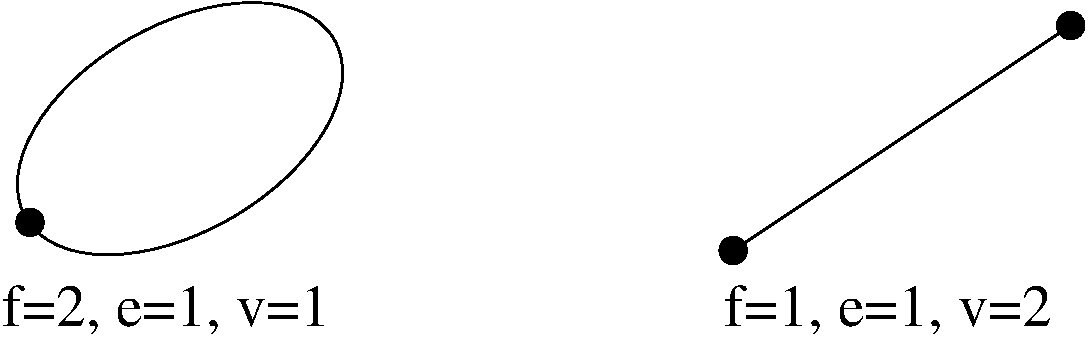
\includegraphics[width=0.4\linewidth,keepaspectratio]{euler1}
\end{center}
\caption{De twee grafen met $e=1$ \label{euler1}}
\end{figure}

1) Onderstel eerst dat $G$ geen kringen bevat.  Neem een maximaal enkelvoudig pad in
$G$; dat pad bevat een knoop $a$ met $\delta(a) = 1$: beschouw de
graaf $G'$ die je verkrijgt door uit $G$ $a$ te verwijderen alsook de
enige boog die erin toekomt; $G'$ heeft 1 knoop en 1 boog minder dan
$G$ en hetzelfde aantal zijvlakken
en $G'$ is nog steeds samenhangend (waarom?),
dus voor $G'$ geldt de formule van Euler, dus ook voor $G$
(zie bijvoorbeeld Figuur~\ref{euler2}).\\
\begin{figure}[ht]
\begin{center}
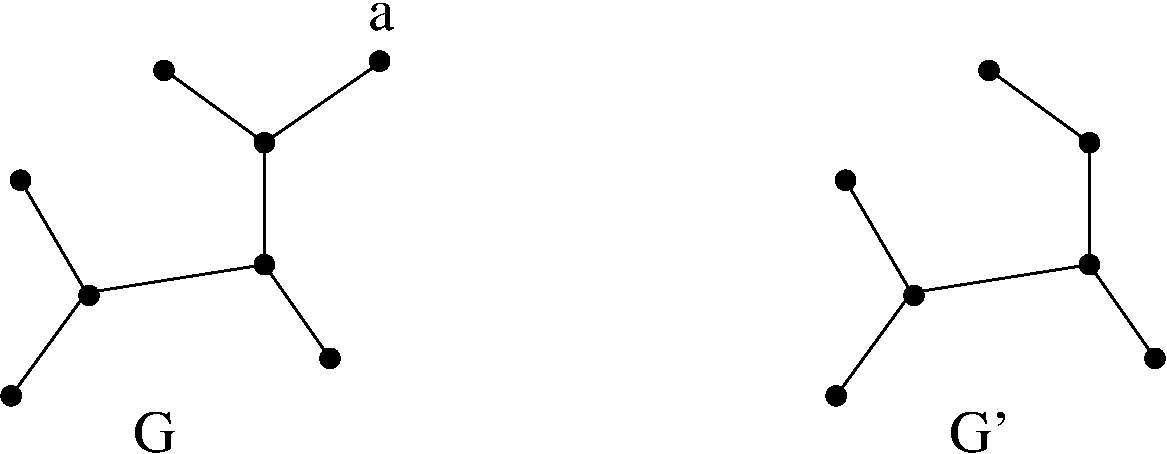
\includegraphics[width=0.4\linewidth,keepaspectratio]{euler2}
\end{center}
\caption{G zonder kringen \label{euler2}}
\end{figure}

2) Stel nu dat $G$ een kring bevat: neem een boog $x$ van een kring van $G$;
verwijder de boog $x$ maar niet de knopen die de boog verbindt; we
verkrijgen $G'$ (zie bijvoorbeeld Figuur~\ref{euler3}). 
\begin{figure}[ht]
\begin{center}
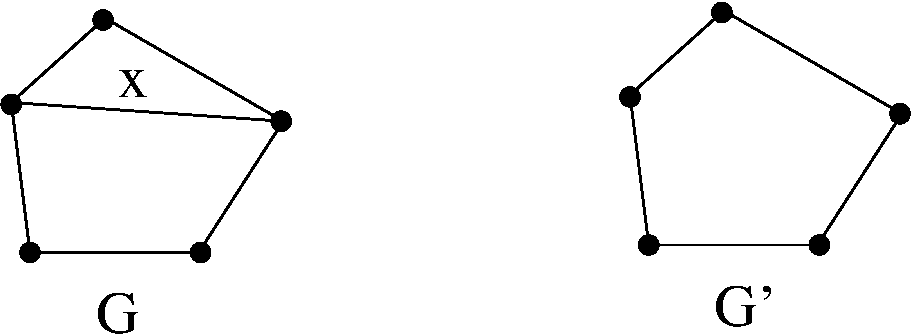
\includegraphics[width=0.4\linewidth,keepaspectratio]{euler3}
\end{center}
\caption{$G$ met een kring \label{euler3}}
\end{figure}
$G'$ heeft $n$ bogen
en nog evenveel knopen als $G$, maar \'{e}\'{e}n zijvlak minder dan $G$;
bovendien is $G'$ samenhangend (waarom?); dus voor
$G'$ geldt (door de inductiehypothese) de formule van Euler en bijgevolg
voor $G$ ook.
\end{proof}

Opmerking: de voorwaarde dat de graaf samenhangend is, is essentieel;
de graaf met juist twee knopen en zonder boog, heeft $f = 1, e = 0, v
= 2$ en de formule van Euler is duidelijk niet geldig. Maar je kan de
formule wel veralgemenen!

De oorsprong van Euler's interesse in de formule was de studie van
ruimtelijke figuren, met name de polyhedra: de veelvlakken; die
interesse bestaat al sinds de Griekse oudheid: in de regelmatige
polyhedra vond men de bouwstenen van de wereld. De formule drukt het
verband uit tussen het aantal vlakken, ribben en hoekpunten van een
polyhedron. De transformatie van een polyhedron naar een vlakke graaf
gaat als volgt: beeld je in dat de polyhedron van rekbaar materiaal is
gemaakt, zoals een ballon en dat de hoekpunten en ribben erop getekend
zijn; prik een gaatje in het midden van een willekeurig vlak, rek dat
gaatje open totdat al het materiaal in een plat vlak ligt. De
resulterende figuur gevormd door de ribben en hoekpunten is de vlakke
graaf; het vlak dat doorprikt werd, komt overeen met het oneindige
``zijvlak''.

 \grijs{\begin{stelling}
$K_{3,3}$ en $K_{5}$ zijn niet vlak.
\end{stelling}}
\begin{proof}
Veronderstel dat $K_{3,3}$ wel een vlakke graaf is.
Laat $\beta$ het aantal bogen voorstellen dat een zijvlak begrenst (tel een
boog $n$ keer als hij $n$ zijvlakken begrenst). Vermits elke boog
maximaal 2 zijvlakken begrenst, hebben we voor elke vlakke graaf $2*e \geq
\beta$ (in het algemeen begrenzen sommige bogen geen zijvlak).

In $K_{3,3}$ heeft elke kring minimaal 4 bogen (waarom?) en dus is
$\beta \geq 4*f$. Samen met de vorige ongelijkheid hebben we dus: $e
\geq 2*f$. Stel dat $K_{3,3}$ vlak is. Door gebruik van de formule van
Euler om in het rechterlid $f$ te elimineren, bekomen we $e \geq 2*(e-v+2)$.
Vul daarin de waarden van $e$ en $v$ in voor $K_{3,3}$ en we
verkrijgen $9 \geq 10$ en contradictie. Bijgevolg is $K_{3,3}$ niet
vlak.

In $K_{5}$ heeft elke kring minimaal 3 bogen \ldots\ en het vervolg van
het bewijs is analoog.
\end{proof}




We hebben vroeger de definitie van isomorfe grafen gezien, maar soms
lijken twee grafen op elkaar zonder dat ze hetzelfde aantal knopen
hebben: als we in het midden van een boog van een graaf een extra
knoop zetten, dan hebben we weinig essentieels aan de graaf veranderd
(als de graaf vlak was, blijft ze vlak; als de graaf samenhangend of
\ldots\ - vul zelf nog wat eigenschappen in - was, behoudt ze die
eigenschap). Daarom is de volgende transformatie op grafen ingevoerd:
drie (verschillende) knopen a,b,c van een graaf liggen op een rij als
er bogen (a,b) en (b,c) bestaan en als er geen andere bogen invallen
in b (anders gezegd: $\delta(b) = 2$). Een \textbf{rijreductie}
bestaat erin om uit de oorspronkelijke graaf de bogen (a,b) en (b,c) en de
knoop b te verwijderen en een nieuwe boog (a,c) toe te voegen: zie
Figuur~\ref{rij1}.

\begin{figure}[ht]
\begin{center}
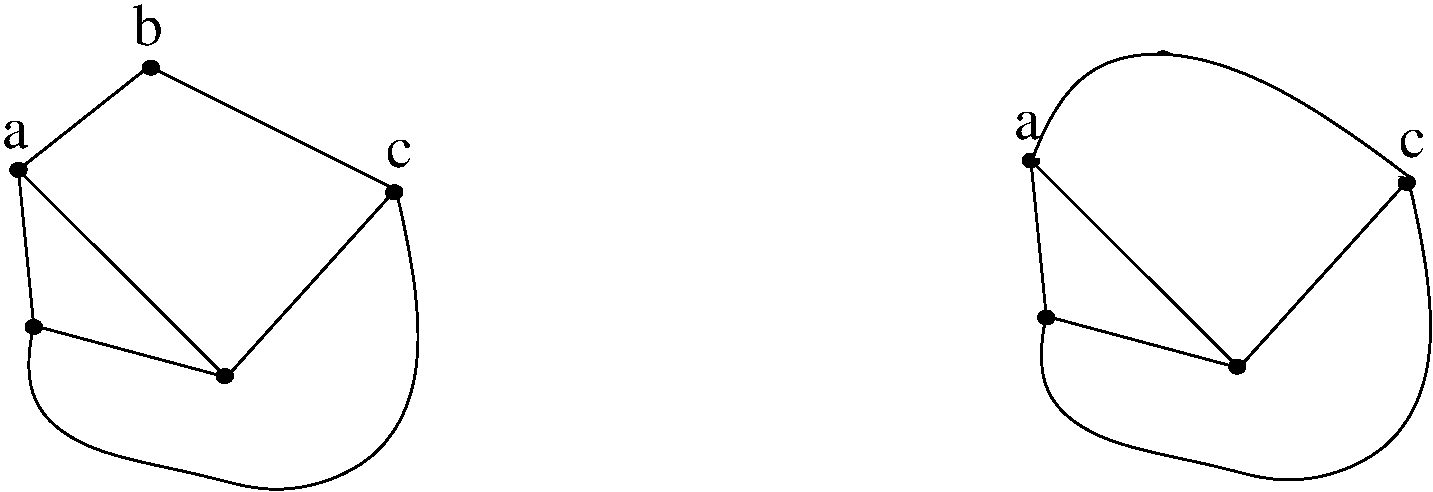
\includegraphics[width=0.4\linewidth,keepaspectratio]{rij1}
\end{center}
\caption{Een rijreductie op een graaf \label{rij1}}
\end{figure}

 \grijs{\begin{definitie}
  \textup{Twee grafen $G_{1}$ en $G_{2}$ worden \textbf{homeomorf}
    genoemd als beide grafen 
    door een rij rijreducties kunnen herleid
    worden tot dezelfde graaf $G$}
\end{definitie}}

 \grijs{\begin{stelling} Stelling van Kuratowski\\
  Een graaf $G$ is vlak als en slechts als $G$ geen deelgraaf bevat 
  die homeomorf is met
  $K_{5}$ 
of
$K_{3,3}$.
\end{stelling}}
\begin{proof}
Indien $G$ een deelgraaf bevat die homeomorf is met $K_{5}$ of
$K_{3,3}$, dan is het duidelijk dat $G$ niet vlak kan zijn, vermits
$K_{5}$ noch $K_{3,3}$ het zijn.
Het bewijs van het omgekeerde valt buiten het bestek van deze cursus.
\end{proof}


Deze stelling maakt $K_{5}$ en $K_{3,3}$ in zekere zin tot de kleinste
niet-vlakke grafen.


\subsection{Het kleuren van grafen}

 \grijs{\begin{definitie}
\textup{Een \textbf{kleuring} van een graaf $(V,E)$ is
een toekenning van een kleur aan elke $v \in V$ zodanig dat de kleuren
van $v$ en $w$ verschillen indien $(v,w) \in E$. Een \mbox{\textbf{n-kleuring}}
is een kleuring met
$n$ of minder
verschillende kleuren. Een
\textbf{minimale} kleuring is een $n$-kleuring met minimale $n$. }
\end{definitie}}

Er zijn heel wat praktische toepassingen van het (minimaal) kleuren
van een graaf. Als voorbeelden

\begin{itemize}
\item
Je moet 4 vergaderingen plannen voor 4 personen A,B,C en D. In de eerste
vergadering zitten A,B; in de tweede A,C, in de derde zitten
B,C,D
en in
de vierde C,D. Wat is het minimale aantal tijdstippen waarop een
vergadering moet gepland worden? Twee vergaderingen moeten op een
verschillend tijdstip doorgaan als eenzelfde persoon aan beide
vergaderingen moet deelnemen.

Je kan het probleem voorstellen door de graaf van figuur
\ref{planning1}: elke knoop stelt een vergadering voor en twee
vergaderingen zijn verbonden als ze niet op hetzelfde tijdstip mogen
doorgaan omdat er iemand in beide vergaderingen moet zijn. Je zoekt er
de kleuring met het kleinste aantal kleuren voor en je hebt het
antwoord (elke nieuwe kleur komt overeen met een nieuw tijdstip).
\begin{figure}[ht]
\begin{center}
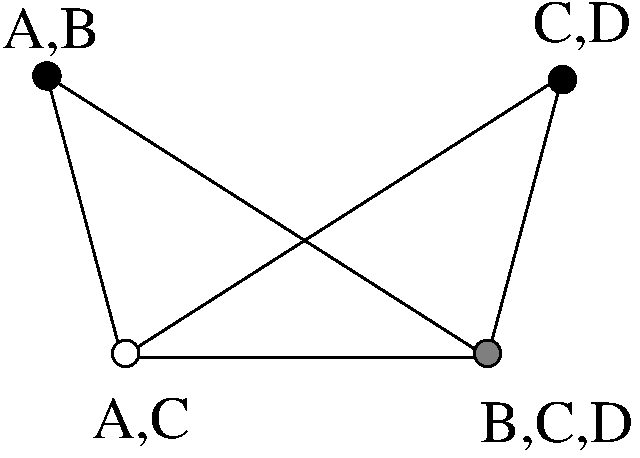
\includegraphics[width=0.2\linewidth,keepaspectratio]{planning1}
\end{center}
\caption{De vergaderingsgraaf met kleuring\label{planning1}}
\end{figure}
\item
Je moet in een warenhuis een aantal goederen opstapelen in de rekken,
maar je mag bepaalde goederen niet naast elkaar zetten: bijvoorbeeld
benzine mag niet naast brood, porno niet naast kuisproducten
enzovoort. Ook hier kan je een graaf opstellen die al die beperkingen
voorstelt en waarbij een kleuring van de graaf het probleem oplost.
\item
Een compiler tracht integer variabelen in machineregisters te
houden in plaats van in het geheugen. Typisch zijn er meer variabelen
dan registers, doch soms kan hetzelfde register gebruikt worden voor
meer dan \'{e}\'{e}n variabele. Bijvoorbeeld in


\parbox{9cm}{
\begin{tabbing}
123 \= 1234 \= 12 \= 12 \= 12 \kill
\> \> \{\\
\> \> \> int i,j,k,l,m;\\
\\
\> \> \> i = 1;\\
\> \> \> j = 2;\\
\> \> \> k = i+j;\\
\> \> \> i = 3;\\
\> \> \> j = 4;\\
\> \> \> l = i+j;\\
\> \> \> m = k+l;\\
\> \> \}
\end{tabbing}
}\\
kan aan i en l hetzelfde register worden toegekend en aan k en m
ook. Dat kan men vinden door de ``interferentie-graaf'' van het stukje
code neer te schrijven, d.w.z. een graaf met als knopen de variabelen
en een boog tussen twee variabelen als ze tegelijkertijd ``in leven''
zijn. We bekomen de graaf in Figuur~\ref{regalloc1}.

\begin{figure}[ht]
\begin{center}
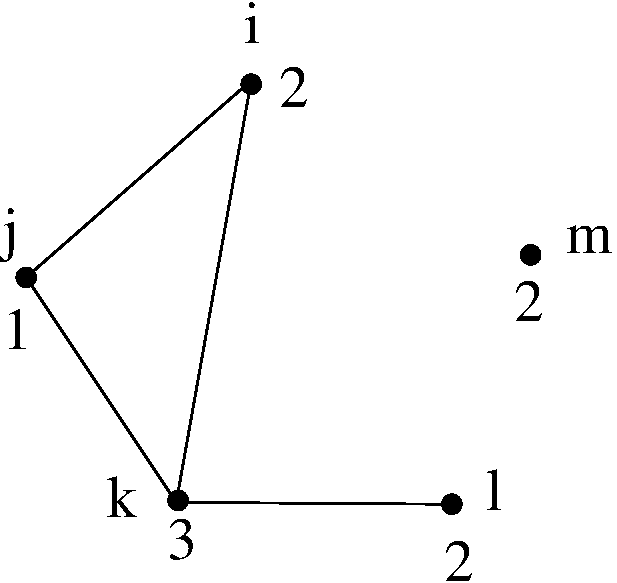
\includegraphics[width=0.2\linewidth,keepaspectratio]{regalloc1}
\end{center}
\caption{De interferentiegraaf met kleuring (in cijfers) \label{regalloc1}}
\end{figure}

Een minimale kleuring geeft aan hoeveel registers je minimaal moet
hebben om elke veranderlijke in een register te bewaren.

\end{itemize}


Een probleem dat ook een praktisch aspect heeft, maar vooral
historisch belangrijk is, is het vier-kleurenprobleem: kan elke
landkaart gekleurd worden met vier verschillende kleuren zodanig dat twee
aangrenzende landen nooit dezelfde kleur hebben? Het probleem werd
voor het eerst gesteld door Francis Guthrie rond 1850. De conjectuur
bleef onbewezen - ondanks verwoede pogingen van menig wiskundige - tot
1976, toen K. Appel en W. Haken bewezen dat er
1936 grafen bestaan
waarvan er minstens \'{e}\'{e}n terug te vinden is in elke minimale
niet $4$-kleurbare graaf en vervolgens bewezen dat zulke grafen niet
minimaal zijn. Beide stappen in het bewijs werden geleverd door een
computerprogramma.

Laten we nu het verband met grafen zien: we zullen van een vlakke
kaart een vlakke graaf maken en het kleuren van de kaart herleiden tot
het kleuren van de graaf.

Een vlakke kaart is een vlakke graaf $G$ waarvan de zijvlakken
ge\"{\i}nterpreteerd worden als landen en de bogen als de grenzen tussen de
landen. De \textbf{duale} graaf van $G$, $G'$ wordt als volgt
geconstrueerd: teken een knoop in elk land van $G$ (ook een knoop voor
het onbegrensde stuk van de kaart) en verbind twee knopen door een
boog indien de twee knopen in aangrenzende landen liggen.

\begin{figure}[ht]
\begin{center}
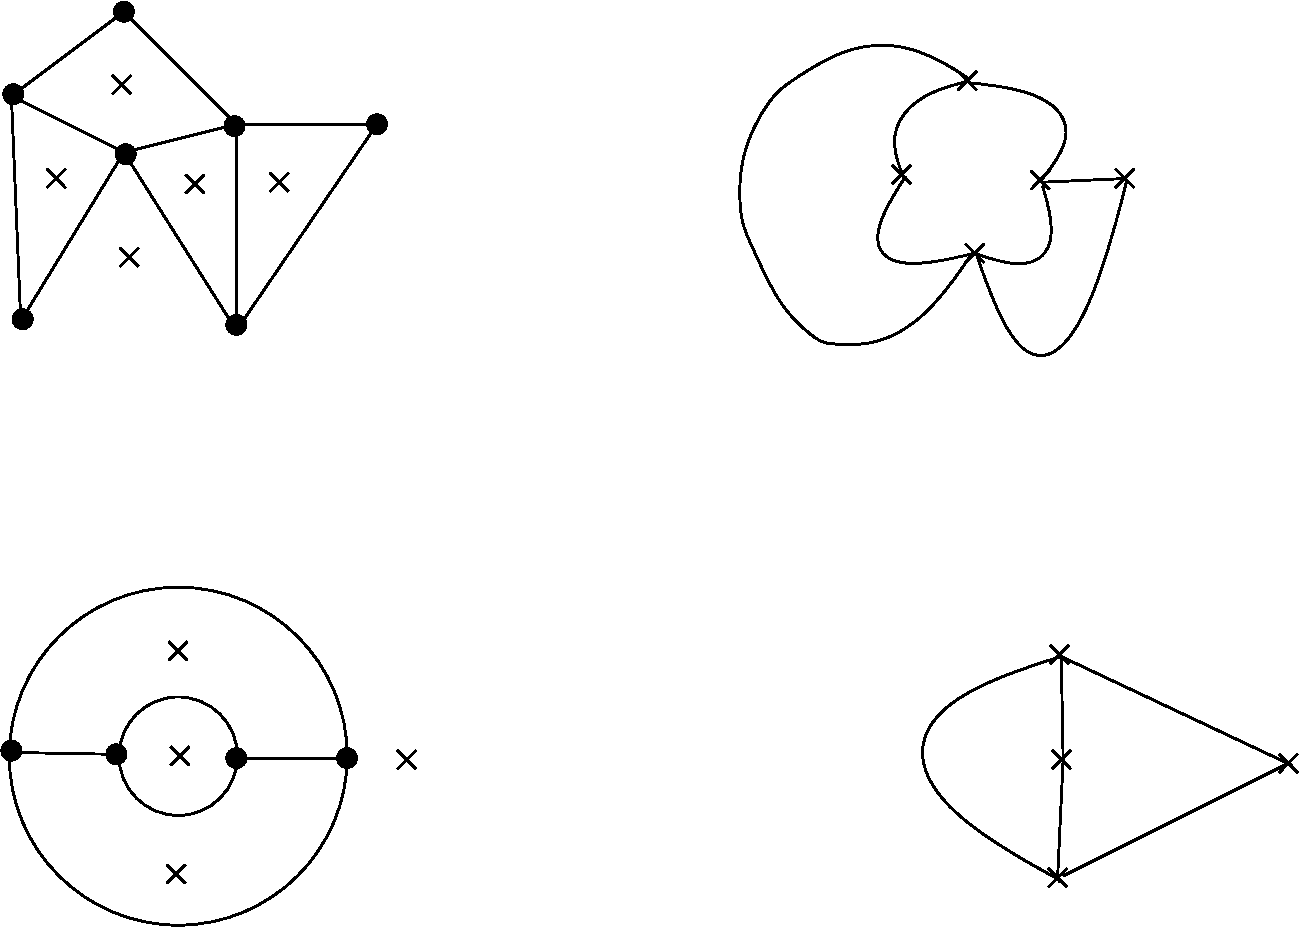
\includegraphics[width=0.6\linewidth,keepaspectratio]{dual1}
\end{center}
\caption{Twee vlakke kaarten en hun duale grafen\label{dual1}}
\end{figure}

Merk op dat de duale graaf van een vlakke kaart vlak is (en enkelvoudig).

 \grijs{\begin{stelling} Voor elke vlakke, enkelvoudige graaf $G$ met meer dan
\'{e}\'{e}n boog geldt dat $e \leq 3*v-6$ \label{euler}
\end{stelling}}
\begin{proof} We bewijzen de stelling enkel voor het geval $G$ ook
samenhangend is: verwijder eerst uit $G$ knopen met graad = 1 (en de
bijbehorende boog), totdat er geen zulke knoop meer bestaat. Je hebt
nu graaf $G'$ die nog steeds vlak, enkelvoudig en samenhangend is, met $f$
zijvlakken en $e'$ bogen en $v'$ knopen. Bovendien is $e-e'=v-v'$ het aantal
verwijderde knopen of bogen: noteer dat aantal door $t$.

1) Indien $e' = 0$ dan moet $v' = 1$; vermits $e > 1$ is $t > 1$; verder
kunnen we schrijven: $e = t$ en $3*v-6 = 3*(v'+t) -6 = 3*t-3$ en
vermits $t \leq 3*t-3$ is ook $e \leq 3*v-6$.

2) $e'$ kan niet gelijk zijn aan 1 of 2 (waarom niet?), dus

3) $e' > 2$; nu
is elke zijvlak begrensd door minstens 3 bogen (vermits er geen lussen
noch parallelle bogen zijn); stel met $\sum$ de som voor van het
aantal bogen in alle zijvlakken, dan is $\sum \geq 3*f$; vermits elke
boog grenst aan exact 2 zijvlakken (waarom?), is ook $\sum = 2*e'$, bijgevolg is
$2*e' \geq 3*f$. Gebruik nu de formule van Euler voor $G'$ om $f$ te
elimineren uit die ongelijkheid en je krijgt: $e' \leq 3*v'-6$ en dus
ook $e'+t \leq 3*(v'+t)-6$ en dus $e \leq 3*v-6$.
\end{proof}

 \grijs{\begin{stelling} In elke vlakke, enkelvoudige graaf bestaat er minstens
\'{e}\'{e}n knoop, zeg $v$, zodanig dat $\delta(v) \leq 5$.
\end{stelling}}
\begin{proof}
Dit is duidelijk waar voor een graaf met 1 of 2 knopen. Stel dat de
stelling niet voldaan is voor een bepaalde graaf met minstens 3
knopen, d.w.z. alle knopen hebben graad 6 of meer, dan is de som van
de graden van alle knopen minstens $6*v$, en bijgevolg $e \geq 3*v$,
hetgeen in tegenspraak is met $e \leq 3*v-6$.
\end{proof}


Het is nu duidelijk dat het kleuren van de vlakke kaart equivalent is
met het kleuren van de duale graaf.
De volgende stelling laat zien dat het kleuren van een vlakke graaf
altijd kan met vijf kleuren:

 \grijs{\begin{stelling} Elke enkelvoudige, vlakke graaf $G(V,E)$
heeft een $5$-kleuring.
\end{stelling}} % uit Townsend
\begin{proof}
We zullen inductie op het aantal knopen gebruiken: indien $G$ juist
\'{e}\'{e}n knoop heeft, is de stelling duidelijk waar.
Veronderstel verder dat $G$ samenhangend is; zoniet is de stelling waar voor
elke component van $G$ en bijgevolg voor $G$.
Stel dat de stelling waar is voor grafen met $n$ knopen; stel $G$ heeft
$n+1$ knopen. Dan bestaat er wegens de vorige stelling minstens
\'{e}\'{e}n knoop $v$ met graad $5$ of minder.\\
Indien de knoop graad 4 of minder heeft, komt $v$ voor in de graaf $G$ als
in Figuur~\ref{5kleuring1}.

\begin{figure}[ht]
\begin{center}
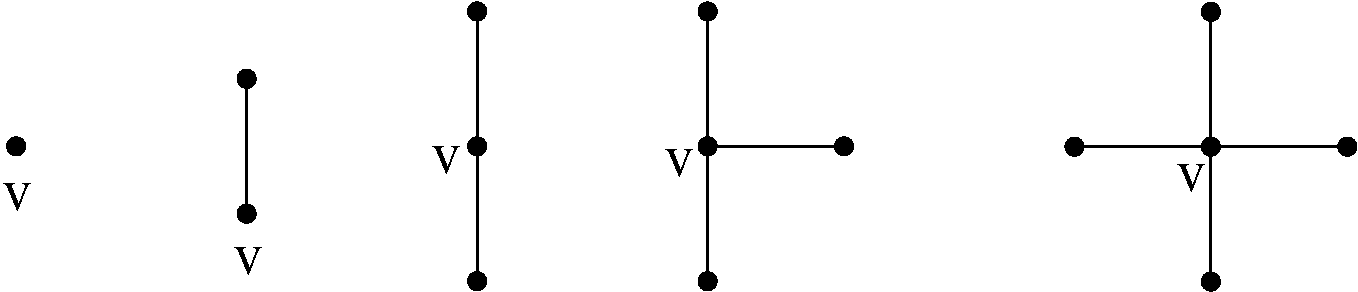
\includegraphics[width=0.6\linewidth,keepaspectratio]{5kleuring1}
\end{center}
\caption{De 5 mogelijkheden waarbij $\delta(v) < 5$ \label{5kleuring1}}
\end{figure}

Beschouw de graaf $G'$ die je verkrijgt door uit $G$ $v$ weg te laten en
alle bogen die in $v$ toekomen. $G'$ voldoet aan de voorwaarden van de
stelling en heeft n knopen, bijgevolg heeft $G'$ een $5$-kleuring. Vermits
$v$ hoogstens 4 buren heeft, kan je aan $v$ een kleur toekennen die
verschillend is van de buren en toch \'{e}\'{e}n van de 5 kleuren is
die voor de $5$-kleuring van $G'$ gebruikt werden.

Indien $\delta(v) = 5$, dan komt $v$ voor in $G$ zoals op de figuur
\ref{5kleuring2}: bij elke buur $w_{i}$ van $v$ is ook de kleur $c_{i}$
($i = 1,\ldots,5$) gezet, zoals bepaald door de $5$-kleuring van $G'$.

\begin{figure}[ht]
\begin{center}
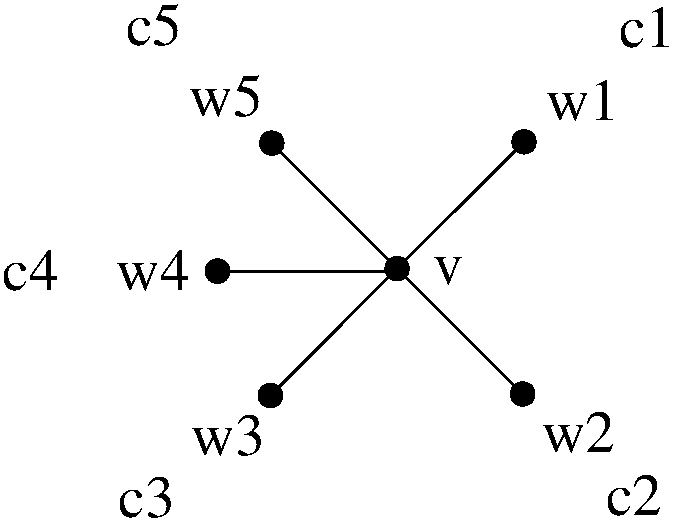
\includegraphics[width=0.25\linewidth,keepaspectratio]{5kleuring2}
\end{center}
\caption{$\delta(v) = 5$ \label{5kleuring2}}
\end{figure}

We moeten nu nog een kleur bepalen voor $v$. Indien de buren van $v$ niet
alle 5 kleuren opgebruiken, kunnen we $v$ een overblijvende kleur geven.

Stel dus dat alle $c_{i}$ verschillend zijn. Beschouw de verzameling
$P_{1,3}$ van alle paden in $G'$ die bij $w_{1}$ beginnen en waarvan de
knopen afwisselend de kleuren $c_{1}$ en $c_{3}$ hebben. Zulke paden
noemen we $c_{1}-c_{3}$ paden.  Er zijn nu twee mogelijkheden:

\begin{description}
\item[$P_{1,3}$ bevat geen pad dat $w_{3}$ bevat:] verander elke
  knoop in $P_{1,3}$ met kleur $c_{1}$ in $c_{3}$ en elke knoop in
  $P_{1,3}$ met kleur $c_{3}$ in $c_{1}$. We hebben nog altijd een
  $5$-kleuring van de graaf G' (waarom?) en nu hebben knopen $w_{3}$ en
  $w_{1}$ beide de kleur $c_{3}$ zodat $v$ geen buur heeft met kleur
  $c_{1}$ dus de nieuwe $5$-kleuring van $G'$ kan uitgebreid worden tot
  een $5$-kleuring van $G$ door aan $v$ de kleur $c_{1}$ toe te kennen.
  
\item[$P_{1,3}$ bevat een pad $p_{1,3}$ dat $w_{3}$ bevat:] construeer
  nu ook $P_{2,5}$: zoals je op de Figuur~\ref{5kleuring3} kan zien,
  kan $P_{2,5}$ geen pad bevatten dat $w_{5}$ bevat; immers, als zulk
  een pad $p_{2,5}$ bestond dan konden de paden $p_{1,3}$ en $p_{2,5}$
  beide uitgebreid worden met de knoop $v$ en kringen vormen in $G$, en
  die kringen zouden mekaar ergens moeten snijden, wat niet mogelijk
  is vermits $G$ vlak is. Nu kunnen we door omwisseling van de kleuren
  van de knopen in $P_{2,5}$ analoog met het eerste geval de stelling
  bewijzen.
\end{description}
\end{proof}

\begin{figure}[ht]
\begin{center}
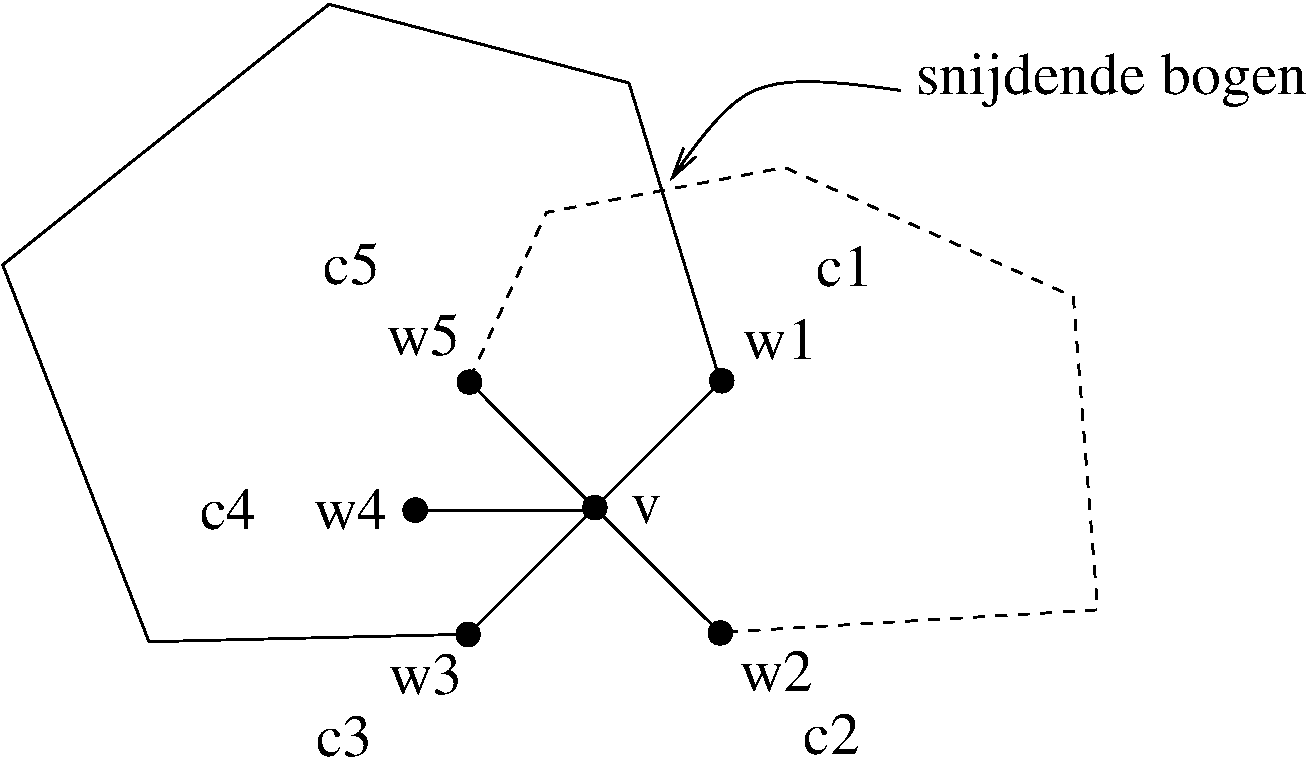
\includegraphics[width=0.4\linewidth,keepaspectratio]{5kleuring3}
\end{center}
\caption{$p_{1,3}$ en $p_{2,5}$ \label{5kleuring3}}
\end{figure}

Appel en Haken {\em bewezen} dat elke vlakke graaf een $4$-kleuring heeft en
bijgevolg {\em bewezen} ze dus de vier-kleurenconjectuur voor vlakke kaarten.

Misschien is dit het juiste ogenblik om even stil te staan bij het
concept van ``een bewijs m.b.v. de computer'': of iets als bewijs
geldt of niet, is grotendeels een sociaal gebeuren; het is misschien
wel juist te beweren dat de mathematische correctheid van een bewijs
onafhankelijk is van of anderen akkoord zijn met die correctheid, maar
een bewijs bestaat maar bij de gratie van een gemeenschap die het
aanvaardt - zelfs als het bewijs later verkeerd blijkt te zijn. Het is
dus aan de gemeenschap (enkel de wiskundige gemeenschap?) dat het
toekomt om in het algemeen computergesteunde bewijzen te accepteren of
niet: men kan zich een tak van de wetenschap voorstellen die enkel
bewijzen geleverd door mensen op papier aanvaardt, net zoals er een tak van
de wiskunde is die wel constructieve maar geen existenti\"{e}le bewijzen
aanvaardt. Het is dus zelfs niet mogelijk enkel gebaseerd op
wetenschappelijke argumenten te beslissen of computergesteunde
bewijzen geldig kunnen zijn of niet. Feit is wel dat naar gelang er
meer bewijzen per computer worden geleverd, de druk groter is om ze te
aanvaarden, vooral als wetenschappers geen andere manier kennen om het
bewijs te leveren, en zeker als er nuttige of bruikbare gevolgen aan
vastzitten.


Anderzijds is het dikwijls mogelijk om een computerbewijs in
principe na te kijken ``met de hand''. 
Een ``hand-matig'' nakijken van het bewijs moet nu het
computerprogramma nakijken, of liever: bewijzen dat het correct is.
Maar een formeel bewijs van de correctheid van grote
computerprogramma's is nog altijd niet doenbaar. Bovendien moet ook de
correctheid van de machine waarop het programma wordt uitgevoerd
bewezen worden \ldots\ misschien iets dat we aan een andere computer kunnen
overlaten?

Om terug te komen op het kleuren van grafen: er zijn (niet-vlakke)
grafen die geen $4$-kleuring hebben; het eenvoudigste voorbeeld is
$K_{n}$ met $n > 4$: daarvoor zijn minimaal $n$ kleuren nodig. Als een
graaf $K_n$ bevat, dan zijn er minstens $n$ kleuren nodig om de graaf
te kleuren. Maar er zijn ook grafen die geen $K_4$ (of groter)
bevatten, en toch meer dan 3 kleuren nodig hebben.

Er zijn ook niet-vlakke grafen die wel een $4$-kleuring hebben: in het
bijzonder heeft $K_{3,3}$ zelfs een $2$-kleuring.

\subsection{Sterk samenhangende componenten: een algoritme van Tarjan}\label{sccs}

In het engels heet het {\em strongly connected components}, en we
korten {\em sterk samenhangende component} af tot SCC. Robert Endre
Tarjan \footnote{Turing award 1986} - de meester algoritmist -
ontwierp in 1972 een bijzonder leuk algoritme om in een gerichte graaf
(een {\em digraph}) de deelverzamelingen knopen te vinden die
onderling bereikbaar zijn. Eerst een voorbeeld met toepassing, dan pas
het algoritme. Gegeven een programma in pseudo-code, waaruit alles is
weggelaten behalve de oproepen van de functies/methodes:
\begin{Verbatim}[frame=single, samepage=true, fontsize=\scriptsize]
main()               venus()                aurochs()           tarpan()
{ venus();           { pluto();             { dodo();           { aurochs();
  aurochs();           venus();               tarpan();         }
}                    }                      }                    
                                                                          
                     pluto()                dodo()              mamoet()
                     { venus();             { tarpan();         { mamoet();
                     }                        mamoet();         }
                                            }
\end{Verbatim}
De {\em oproepgraaf} (call graph) is de gerichte graaf in Figuur
\ref{vbtarjan} waarin de nodes de procedures zijn en een gerichte boog
van A naar B betekent: A roept B op\footnote{Denk daarover even na: is
dat echt waar ?}. Oproepen van een procedure naar zichzelf hebben we
weggelaten.

% \clearpage

\begin{figure}[h]
\begin{center}
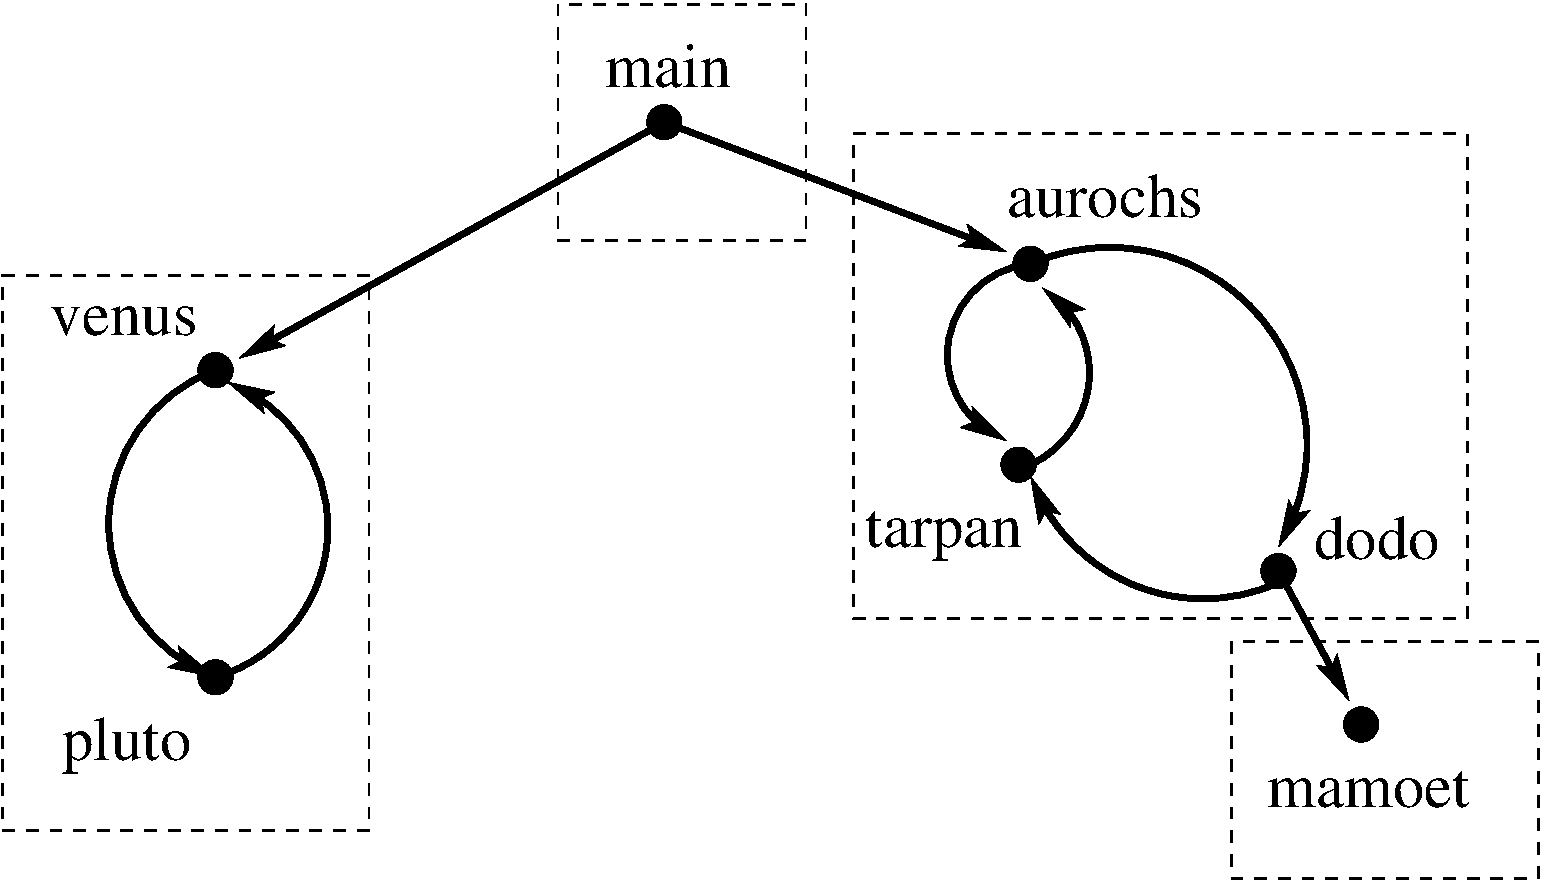
\includegraphics[height=0.2\textheight,keepaspectratio]{vbtarjan}
\caption{De gerichte oproepgraaf die bij het programma hoort}\label{vbtarjan}
\end{center}
\end{figure}


De SCCs daarvan laten toe om het programma op te delen in kleinere
stukken waarvan de analyse onafhankelijk kan gebeuren, en/of op een
goede manier sequentieel gepland. Met analyse bedoelen we hier zaken
als complexiteit, programma-invarianten (voor correctheid), data-flow
en liveness analyse (voor optimizatie) ... Buiten die context zijn er
ook heel wat toepassingen van SCCs.

In Figuur~\ref{vbtarjan} zijn de SCCs al aangeduid met een rechthoek
rond elke SCC: elke knoop behoort tot exact \'{e}\'{e}n SCC. Probeer
dat in te zien of te bewijzen.

De versie in Algoritme~\ref{alg:tarjan} is aangepast van Wikipedia\footnote{
http://en.wikipedia.org/wiki/Tarjan's\_strongly\_connected\_components\_algorithm,
 28-7-2014}.
%
Elke knoop $v$ heeft 4 velden: de booleans instack en visited die
initi\"eel FALSE zijn, en de integers index en lowlink die op tijd
ge\"{i}nitialiseerd worden.  Hun selectie wordt aangeduid bv. door
$v.visited$.

\begin{algorithm}[h]
\begin{algorithmic}

\Function {tarjan}{}
    \State{index := 1;}
    \ForAll{$v \in V \wedge (\neg v.visited)$}
    \State{strongconnect(v);}
    \EndFor
\EndFunction
~\\
\Function {strongconnect}{v}
\State{v.visited := TRUE;}
\State{v.index := v.lowlink := index++;}
\State{push(v); v.instack := TRUE;}
~\\
\ForAll {$(v,w) \in E$}
       \If {$\neg w.visited$};
       \State{strongconnect(w);}
       \State{v.lowlink  := min(v.lowlink, w.lowlink);}
       \ElsIf {w.instack}
       \State{v.lowlink  := min(v.lowlink, w.index)}
       \EndIf
\EndFor
% ~\\
    \If{v.lowlink == v.index}
    \State{start a new SCC}
    \Repeat
         \State{w := pop(); w.instack := FALSE;}
         \State{add w to current SCC}
    \Until {w == v}
    \State{output current SCC}
    \EndIf
\EndFunction

  \end{algorithmic}
  \caption{Tarjan's algoritme om SCCs te berekenen}
  \label{alg:tarjan}
\end{algorithm}


Argumenteer zelf de correctheid en de eindigheid van dit algoritme.

Donald E. Knuth\footnote{Turing award in 1974}
zegt\footnote{http://www.informit.com/articles/article.aspx?p=2213858\&WT.mc\_id=Author\_Knuth\_20Questions}
dat Tarjan's algoritme zijn favoriete algoritme is, o.a. omdat het ook
nog topologisch sorteert als een bijproduct. Zie je dat in het
algortime ?

\newpage

\section{Bomen}

\subsection{Inleiding}

 \grijs{\begin{definitie} Boom\\
  \textup{ Een \textbf{boom} is een enkelvoudige graaf met de eigenschap
    dat er tussen elke twee verschillende knopen een uniek enkelvoudig pad
    bestaat. }
\end{definitie}}

Een willekeurige knoop van een boom kan aangewezen worden als de
\textbf{wortel}.

 \grijs{\begin{definitie} Hoogte van een knoop\\
  \textup{ 
De 
 \textbf{hoogte van een knoop} $v$ in een boom met wortel
    $w$, is het aantal bogen in het pad van $w$ naar $v$. }
\end{definitie}}

 \grijs{\begin{definitie} Hoogte van een boom\\
  \textup{ 
De 
\textbf{hoogte van een boom} is het maximum van de
    hoogtes van zijn knopen. }
\end{definitie}}

\begin{figure}[ht]
\begin{center}
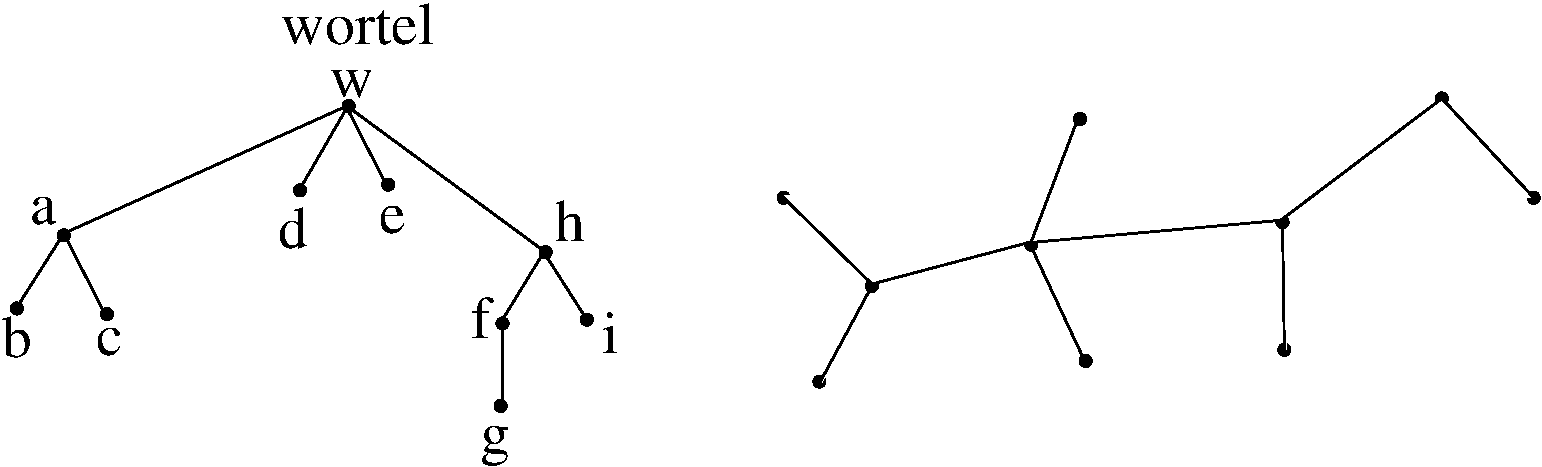
\includegraphics[width=0.5\linewidth,keepaspectratio]{bomen1}
\end{center}
\caption{Voorbeelden van bomen \label{bomen1}}
\end{figure}


Figuur~\ref{bomen1} laat een boom met een wortel $w$ zien en een boom
zonder wortel. De hoogtes van $a,b,c,d,e,f,g,h,i$ en $w$ zijn
respectievelijk 1,2,2,1,1,2,3,1,2 en 0.

\begin{figure}[ht]
\centering
\mbox{
\subfigure[Beslissingsboom]{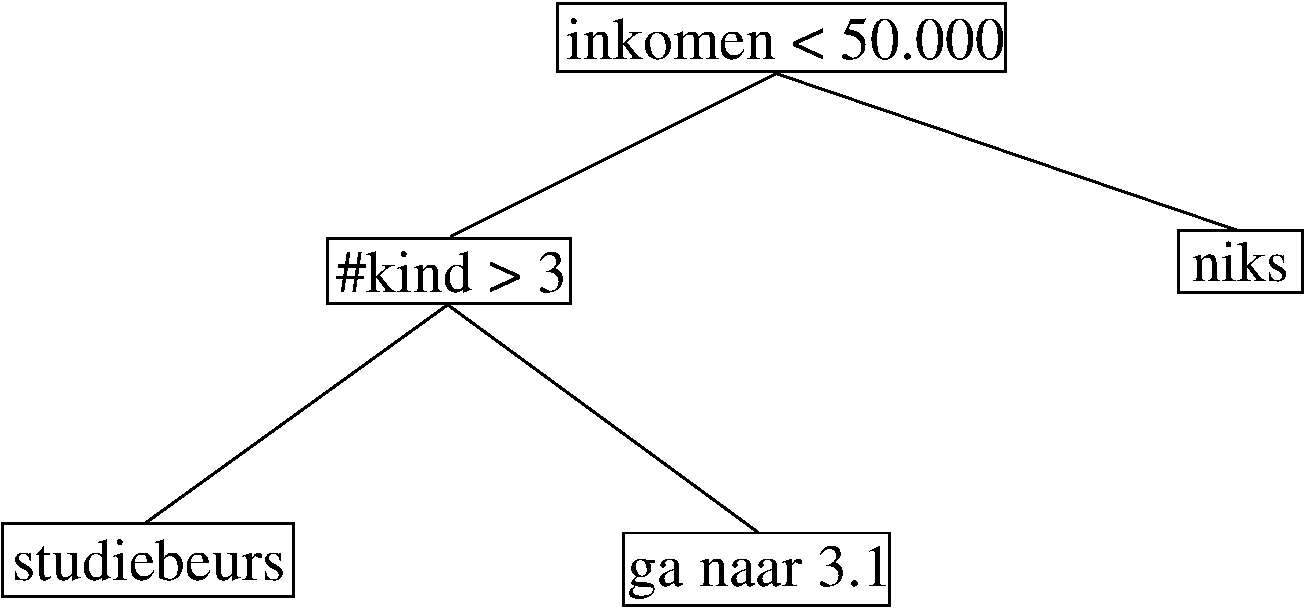
\includegraphics[width=0.5\linewidth,keepaspectratio]{decisiontree1} \label{decisiontree1}} %\quad
\subfigure[Voorstelling van $(3+1) *5 - 7/3$]{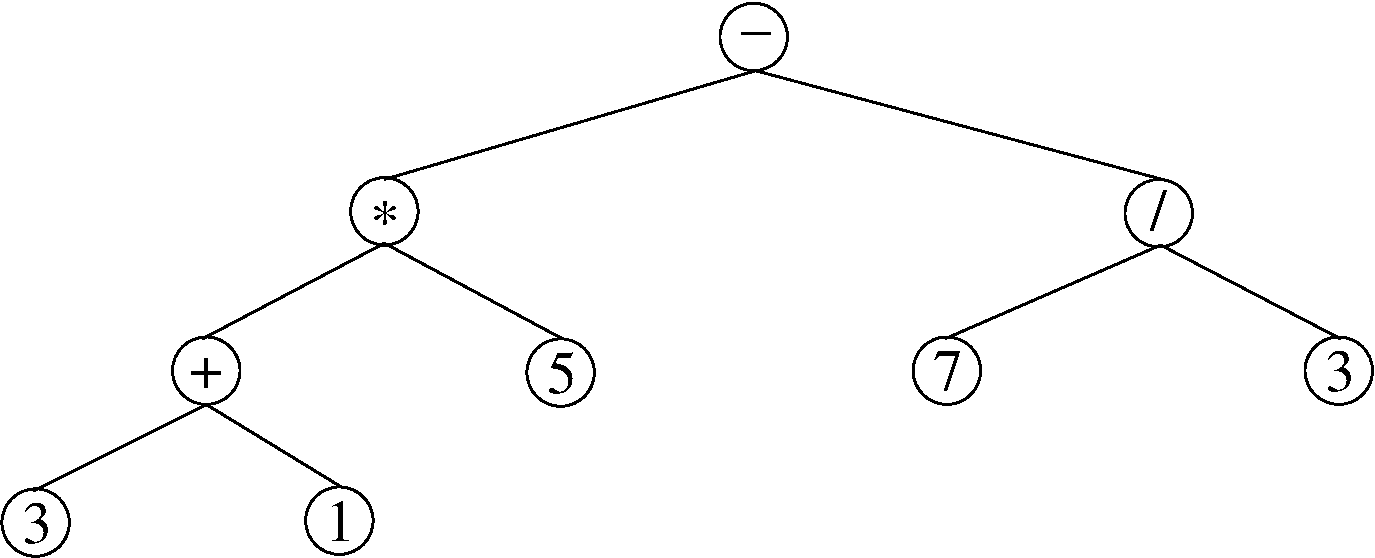
\includegraphics[width=0.5\linewidth,keepaspectratio]{expr1} \label{expr1} }}
\caption{Nuttige bomen}
\end{figure}


Figuur~\ref{decisiontree1} toont een beslissingsboom: elke knoop bevat
een test. De wortel is de knoop met de test ``$inkomen < 50.000$'';
afhankelijk van of de test positief of negatief uitvalt, ga je naar
links of rechts waar je meer testen vindt of advies/antwoord op de
vraag ``heb ik recht op een studiebeurs?''.

Figuur~\ref{expr1} toont de boomvoorstelling van de rekenkundige
uitdrukking $(3+1) *5 - 7/3$.

\subsection{Eigenschappen van bomen}

De volgende stelling geeft een aantal equivalente karakterisaties van
bomen:

 \grijs{\begin{stelling}
  Voor een enkelvoudige graaf $T$ met $n$ knopen geldt dat\\
 $(a) \Leftrightarrow
  (b) \Leftrightarrow (c) \Leftrightarrow (d)$ met \\[2mm]
(a) $T$ is een boom\\
(b) $T$ is samenhangend en bevat geen kring\\
(c) $T$ is samenhangend en heeft $(n-1)$ bogen\\
(d) $T$ bevat geen kring en heeft $(n-1)$ bogen
\end{stelling}}
\begin{proof}
\begin{itemize}
\item $(a) \Rightarrow (b)$: als $T$ een boom is bestaat er een pad
  tussen elke twee knopen, bijgevolg is $T$ samenhangend; er kan geen
  kring zijn in $T$ anders zouden sommige knopen door meer dan
  \'{e}\'{e}n enkelvoudig pad verbonden zijn
\item $(b) \Rightarrow (c)$: we bewijzen door inductie op $n$ dat $T$
  $(n-1)$ bogen heeft; voor $n=1$ heeft $T$ nul bogen en de basis voor de
  inductie is waar; stel dat elke samenhangende graaf, zonder kringen en
  met $n$ knopen $(n-1)$ bogen heeft;
  neem een graaf $S$ met $(n+1)$ knopen, zonder kringen en samenhangend;
  kies een
  enkelvoudig
  pad $P$ van maximale lengte in $S$ (is dit mogelijk?); vermits
  er geen kringen zijn in $S$, bevat $P$ een knoop $v$ met $\delta(v) = 1$
  (indien $\delta(v) > 1$ dan kon het pad $P$ uitgebreid worden en dan
  was het niet maximaal); beschouw $S_{*}$ de graaf die je verkrijgt
  door uit $S$ knoop $v$ (en zijn boog) weg te laten; $S_{*}$ heeft $n$
  knopen, heeft geen kring en is samenhangend en door inductie bevat
  $S_{*}$ $(n-1)$ bogen; bijgevolg bevat $S$ $n$ bogen
\item $(c) \Rightarrow (d)$: stel dat $T$ een kring bevat, dan kunnen we
  bogen (minstens \'{e}\'{e}n! en geen knopen!) verwijderen uit $T$
  totdat de resulterende graaf $T_{*}$ kringloos is maar nog steeds
  samenhangend; nu is $T_{*}$ zonder kringen, samenhangend en bevat $n$
  knopen en we kunnen bijgevolg het resultaat $(b) \Rightarrow (c)$
  gebruiken: $T_{*}$ bevat $(n-1)$ bogen; daaruit volgt dat $T$ strikt
  meer dan $(n-1)$ bogen had, in tegenspraak met de onderstelling in
  (c); daaruit volgt dat $T$ geen kring bevat
\item $(d) \Rightarrow (a)$: we moeten bewijzen dat $T$ samenhangend is
  en dat er een uniek pad bestaat tussen elke twee knopen; we kunnen
  een partitie maken van $T$ in zijn componenten $\{T_{i}\}_{i=1}^{k}$;
  stel dat het aantal knopen van $T_{i}$ gelijk is aan $n_{i}$; elk
  van de $T_{i}$ is samenhangend en kringloos en heeft bijgevolg
  $(n_{i}-1)$ bogen; dus: $(n-1) = \sum_{i=1}^{k} (n_{i}-1) =
  \sum_{i=1}^{k} (n_{i}) - k = n - k$; daaruit volgt dat $k=1$ en dus is
  $T$ samenhangend; stel nu dat er twee paden van $a$ naar $b$ bestaan, 
  dan kan je met die paden een kring vormen;
  maar $T$ is kringloos, dus is elk pad tussen twee knopen uniek;
  bijgevolg is $T$ een boom

\end{itemize}
\end{proof}


De stelling is o.a. belangrijk om de volgende reden: rondlopen in een
graaf die geen boom is, is gevaarlijk omdat je in een kring kan
terecht komen en op die manier in een oneindige lus. Om dat te
vermijden, zou je altijd moeten bijhouden waar je al geweest bent. De
stelling zegt o.a. dat voor een boom je een pad altijd kan uitbreiden
``voorwaarts'' en vermits er geen kringen zijn, zal je op de duur niet
meer verder kunnen. Bijgevolg, als je weet dat je met een boom te doen
hebt, dan kan je (eigenlijk zou je moeten) van die eigenschap gebruik
maken bij het programmeren van toepassingen met die datastructuur.


 \grijs{\begin{definitie} Terminologie i.v.m. bomen\\ 
\textup{Laat $T$ een boom zijn
met wortel $v_{0}$; laten $x$, $y$ en $z$ knopen zijn in $T$ en $(v_{0},
v_{1}, \ldots , v_{n})$ een pad in $T$, dan} {\rm
\begin{verse}
%\begin{itemize}
%\item
\hspace*{1ex}$\bullet$ 
$v_{n-1}$ is de \textbf{ouder} van $v_{n}$; we spreken soms ook over vader of 
moeder;
 
%\item
\hspace*{1ex}$\bullet$
$v_{0}$ \ldots\ $v_{n-1}$ zijn \textbf{voorouders} van $v_{n}$ en $v_{n}$ is
een \textbf{afstammeling} van $v_{0}$ \ldots\ $v_{n-1}$
%\item

\hspace*{1ex}$\bullet$
$v_{n}$ is een \textbf{kind} van $v_{n-1}$; we spreken soms van zoon of dochter
%\item

\hspace*{1ex}$\bullet$
als $x$ en $y$ 
kinderen
zijn van $z$, dan zijn $x$ en $y$ broers of 
zusters (in het Engels: siblings)
%\item

\hspace*{1ex}$\bullet$
als $x$ geen enkel kind heeft, dan is $x$ een \textbf{blad} of \textbf{eindknoop}
%\item

\hspace*{1ex}$\bullet$
als $x$ geen blad is, is $x$ een \textbf{inwendige knoop}
%\item

\hspace*{1ex}$\bullet$
de deelgraaf van $T$ die een knoop $x$ bevat en al de afstammelingen van
$x$,
is de \textbf{deelboom} van $T$ met wortel 
$x$\footnotemark
%\end{itemize}
\end{verse}}
\end{definitie}}
\footnotetext{In feite moeten we bewijzen dat die deelgraaf een boom is!}

\begin{figure}[ht]
\begin{center}
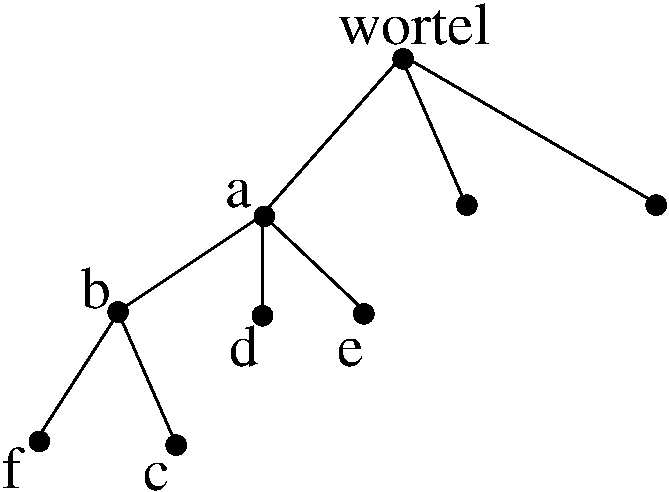
\includegraphics[width=0.25\linewidth,keepaspectratio]{boom1}
\end{center}
\caption{Voorbeeldboom \label{boom1}}
\end{figure}


Voorbeelden van al die terminologie: voor Figuur~\ref{boom1} geldt dat
\begin{itemize}
\item
$c,d,e$ zijn bladeren of eindknopen
\item
$a$ is de ouder van $d$
\item
$b,c,f$ zijn de afstammelingen van $a$
\item
$a,$wortel zijn de voorouders van $b$
\item
$b,d,e$ zijn siblings
\item
$a,b$ zijn inwendige knopen
\item
de deelboom met wortel $a$ bevat de knopen $a,b,c,d,e,f$
\end{itemize}

Soms vinden we de volgorde van de kinderen van een knoop in een boom
belangrijk, in het bijzonder is dat zo bij een binaire boom.

 \grijs{\begin{definitie} Binaire boom\\
\textup{Een \textbf{binaire boom} is een boom met een wortel en
waarvan elke knoop 0, 1 of 2 kinderen heeft; wegens de manier waarop
binaire bomen getekend en gebruikt worden, spreekt men van een
linkerkind (verbonden door de linkertak met de ouder) en een
rechterkind (\ldots); de orde van de takken is dus belangrijk.
}
\end{definitie}}

Je zag al een binaire boom in Figuur~\ref{decisiontree1}: het is daar
belangrijk te weten of je links of rechts moet gaan bij een positief
antwoord op de test in de knoop.

 \grijs{\begin{definitie} Volledige binaire boom\\
\textup{Een \textbf{volledige binaire boom} is een binaire boom
waarvan elke inwendige knoop juist twee kinderen heeft.
}
\end{definitie}}

\begin{figure}[ht]
\begin{center}
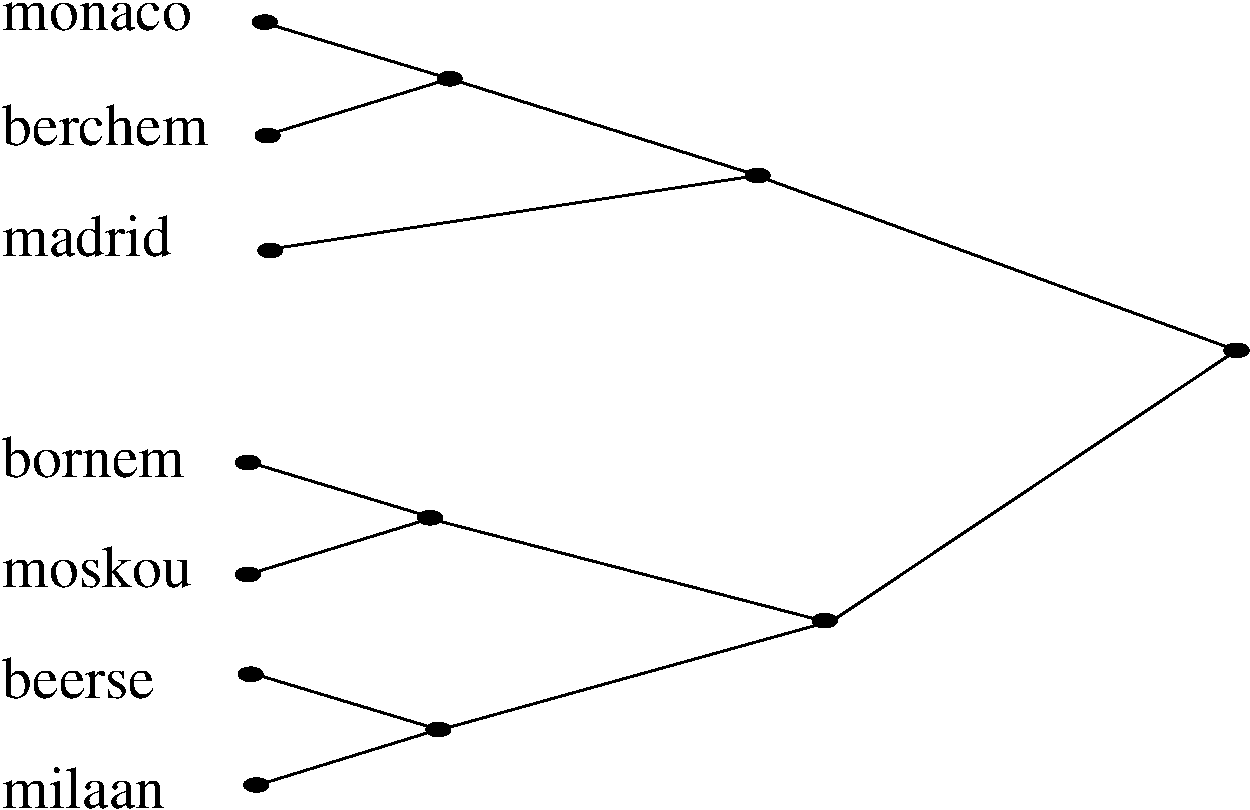
\includegraphics[width=0.5\linewidth,keepaspectratio]{tornooi1}
\end{center}
\caption{Tornooiboom \label{tornooi1}}
\end{figure}


Een voorbeeld van een volledige binaire boom vinden we in de
boomvoorstelling van de directe uitschakeling in een tornooi: figuur
\ref{tornooi1}.

 \grijs{\begin{stelling}
\label{relatiebladinwendig}
Indien $T$ een volledige binaire boom is met $i$ inwendige knopen, dan heeft
$T$ $(i+1)$ bladeren en $(2i+1)$ knopen.
\end{stelling}}
\begin{proof} Elke inwendige knoop heeft 2 kinderen, er zijn dus
$2i$ kinderen in $T$; er is ook \'{e}\'{e}n knoop die geen kind is,
namelijk de wortel, bijgevolg zijn er $2i+1$ knopen. Vermits een blad
geen inwendige knoop is en vice versa, en vermits elke knoop een blad
is of een inwendige knoop, hebben we ook dat het aantal bladeren
gelijk is aan $2i+1 - i = i+1$
\end{proof}



Bij een tornooi met directe uitschakeling met $n$ deelnemers, kan je de
vraag stellen: hoeveel matchen moeten er ingericht worden om de
winnaar te kunnen aanduiden? De tornooiboom heeft $n$ bladeren,
bijgevolg heeft hij $n-1$ inwendige knopen en dat is ook het aantal
matchen.

 \grijs{\begin{stelling}
\label{relatiehoogtebladeren}
Indien $T$ een binaire boom is met hoogte $h$ en $t$ bladeren, dan $\log_2(t)
\leq h$ (of $t \leq 2^h$).
\end{stelling}}
\begin{proof}
We bewijzen de stelling door inductie op $h$ en door de deelbomen van $T$
te beschouwen: voor $h=0$ hebben we \'{e}\'{e}n blad (de wortel), dus
$t=1=2^h=2^0$ en de stelling is voldaan.

Stel $h > 0$; beschouw $T_{l}$ en $T_{r}$ de linker- en
rechterdeelboom van de wortel van $T$. $T_{l}$ of $T_{r}$ kunnen leeg zijn,
maar niet beide. Onderstel eerst dat $T_{r}$ leeg is: dan is
$h_{l} = h-1$ en door inductie is $t_{l} \leq 2^{h_{l}}$; vermits 
$t_{l} = t$ verkrijgen we $t \leq 2^{h-1}\leq 2^h$. 

Het geval dat $T_{l}$ leeg is, is analoog.

Stel $T_{l}$ noch $T_{r}$ leeg, dan is $h_{l} \leq h-1$ en door
inductie is $t_{l} \leq 2^{h_{l}}$; analoog is $t_{r} \leq 2^{h_{r}}$ en dus
$t=t_{l} + t_{r} \leq 2^{h_{l}} + 2^{h_{r}}\leq 2^{h-1}+2^{h-1}=2^h$.
\end{proof}

 \grijs{\begin{stelling} Voor een binaire boom $T$ met $n$ knopen en hoogte $h$,
is $\log_2(n+1) \leq h+1$
\label{relatiehoogtenodes}
\end{stelling}}
\begin{proof}
Breid eerst de boom $T$ uit tot een boom $T'$ als volgt:
\begin{itemize}
\item
hang aan elk blad een linker- en een rechtertak
\item
als een 
inwendige
knoop een linkertak mist, voeg een linkertak toe
\item
als een 
inwendige
knoop een rechtertak mist, voeg een rechtertak toe
\end{itemize}

$T'$ heeft nu $n$ inwendige knopen (alle originele knopen van $T$) en hoogte
$(h+1)$; vermits $T'$ volledig en binair is, kunnen we stelling
\ref{relatiebladinwendig} toepassen en besluiten dat $T'$ $(n+1)$ bladeren
heeft en door Stelling~\ref{relatiehoogtebladeren} besluiten dat $lg(n+1)
\leq h+1$
\end{proof}

Figuur~\ref{uitbreiding1} toont een boom en zijn uitbreiding zoals
gedefinieerd in Stelling~\ref{relatiehoogtenodes}: de toegevoegde knopen
zijn getekend als een zwart rechthoekje. Merk ook op dat als de
oorspronkelijk boom al volledig is, de uitbreiding toch verschilt!

\begin{figure}[ht]
\begin{center}
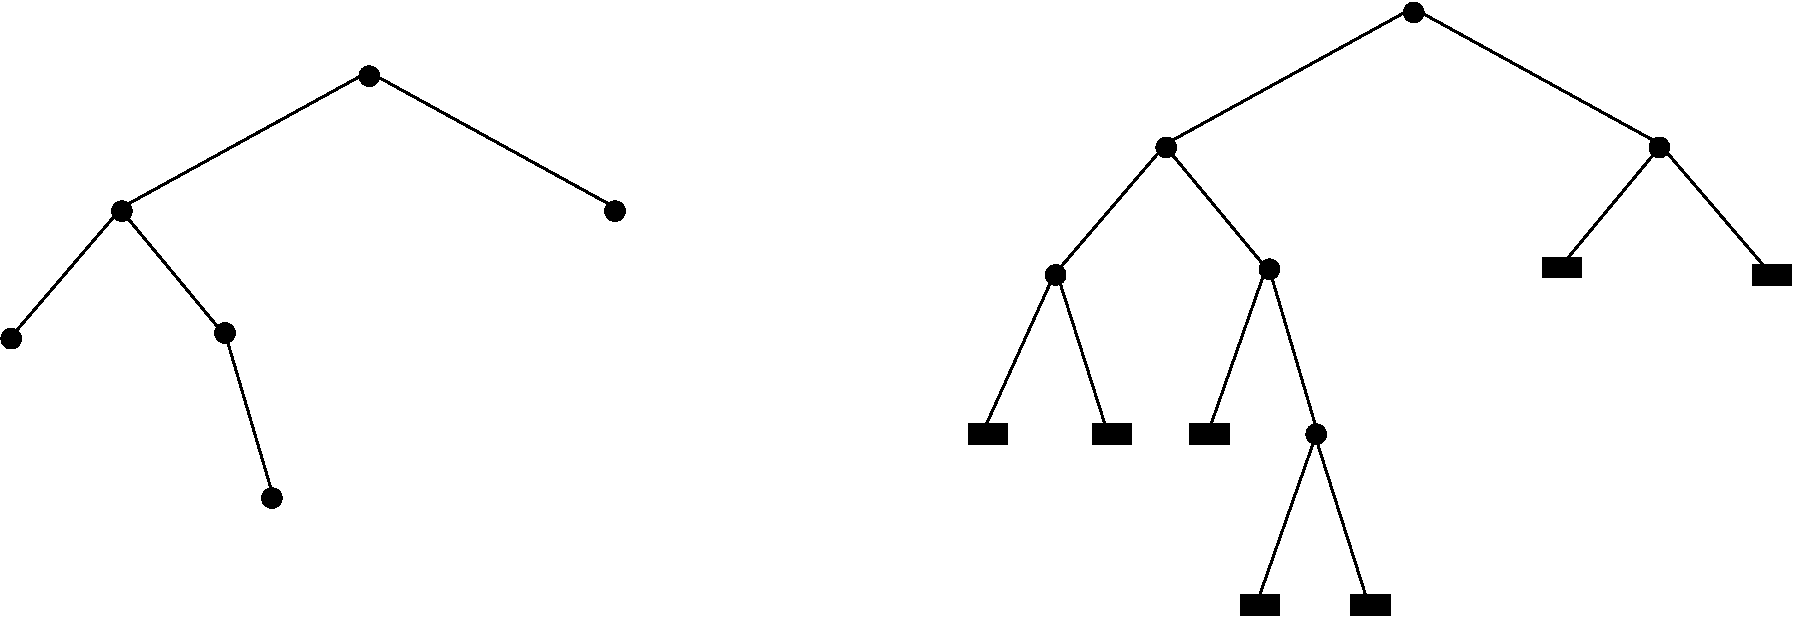
\includegraphics[width=0.6\linewidth,keepaspectratio]{uitbreiding1}
\end{center}
\caption{Een binaire boom en zijn uitbreiding tot een volledige binaire boom\label{uitbreiding1}}
\end{figure}

 \grijs{\begin{definitie} Binaire zoekboom\\
\textup{Een \textbf{binaire zoekboom} is een binaire boom waarin met
elke knoop $v$ een waarde $w(v)$ is geassocieerd (bv. een getal) zodanig
dat als $l$ behoort tot de linker-- en  $r$ tot
de rechterdeelboom van $v$, dat dan $w(l) < w(v) < w(r)$
}
\end{definitie}}


Een binaire zoekboom wordt ook soms gesorteerde binaire boom genoemd.

Figuur~\ref{binboom1} toont een binaire zoekboom waarin de waarde van
de knopen woorden zijn; de orde is alfabetisch.

\begin{figure}[ht]
\begin{center}
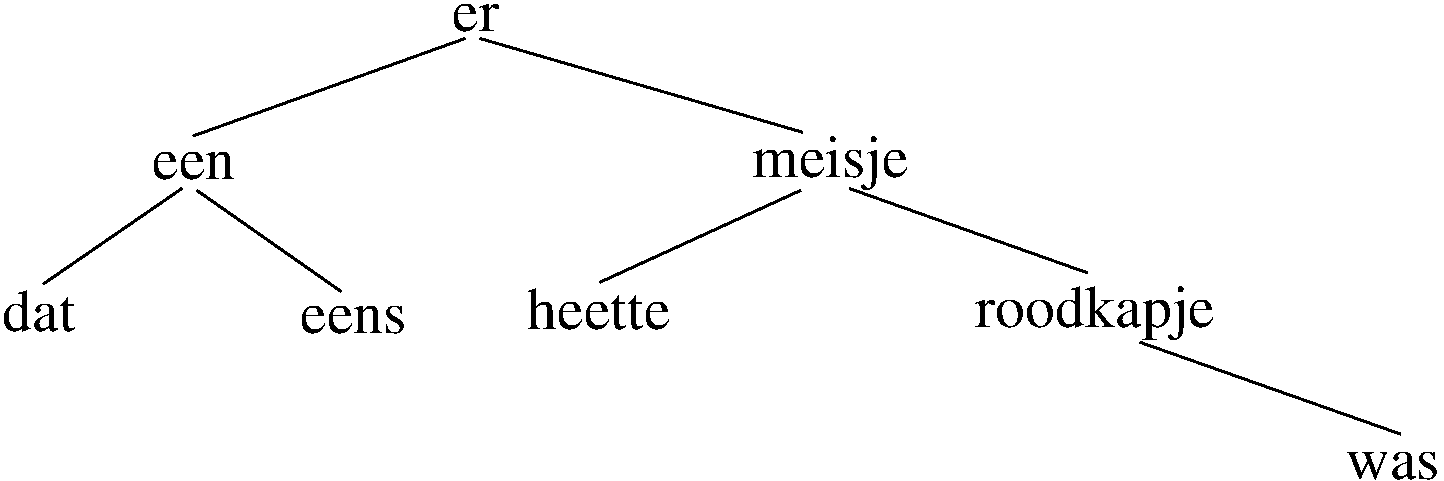
\includegraphics[width=0.6\linewidth,keepaspectratio]{binboom1}
\end{center}
\caption{Een binaire zoekboom voor de woorden uit de zin
``Er was eens een meisje dat Roodkapje heette'' \label{binboom1}}
\end{figure}

Het volgende algoritme zoekt of een bepaalde waarde aanwezig is in een
binaire zoekboom: het algoritme is geschreven als een procedure die
TRUE teruggeeft als de waarde gevonden is, anders FALSE.

% Bart - java code van gemaakt

\parbox{9cm}{
\begin{tabbing}
123456789 \= 12 \= 12 \= 12 \= 12 \= 12 \= 12 \kill
\> boolean zoek(T boom, W waarde);\\
\> \{\\
\> \> P = wortel(T);\\
\> \> doevoort = not(empty(T));\\
\> \> zoek = FALSE;\\
\> \> while (doevoort)\\
\> \> \{\\
\> \> \> if (waarde(P) == W)\\
\> \> \> \> \{ \\
\> \> \> \> \> doevoort = FALSE;\\
\> \> \> \> \> zoek = TRUE;\\
\> \> \> \> \}\\
\> \> \> else\\
\> \> \> if (waarde(P) $<$ W)\\
\> \> \> \> P = rechterkind(P);\\
\> \> \> else P = linkerkind(P);\\
\> \> \> if (empty(P)) \\
\> \> \> \> doevoort = FALSE\\
\> \> \}\\
\> \}
\end{tabbing}
}

We kunnen de complexiteit van dit algoritme uitdrukken in het aantal
keer dat het lichaam van de lus wordt uitgevoerd. In het slechtste
geval zit de gezochte waarde niet in de boom en zoeken we langs het
langste pad, vertrekkend aan de wortel; dat pad heeft een lengte die
gelijk is aan de hoogte h van de boom en de lus wordt dus $h+1$ keer
uitgevoerd. Uit Stelling~\ref{relatiehoogtenodes} weten we dat
$lg(n+1) \leq h+1$ en voor een vaste n kunnen we het slechtste geval
dus niet beter maken dan $lg(n+1)$. Door de boom zo goed mogelijk te
``balanceren'' verkrijgen we een slechtste geval dat gelijk is aan
$\lceil lg(n+1) \rceil$. Een voorbeeld van twee binaire bomen met
dezelfde knopen zie je in Figuur~\ref{balanced1}: de rechterboom is
beter gebalanceerd dan de linkerboom en is dus minder hoog.

\begin{figure}[ht]
\begin{center}
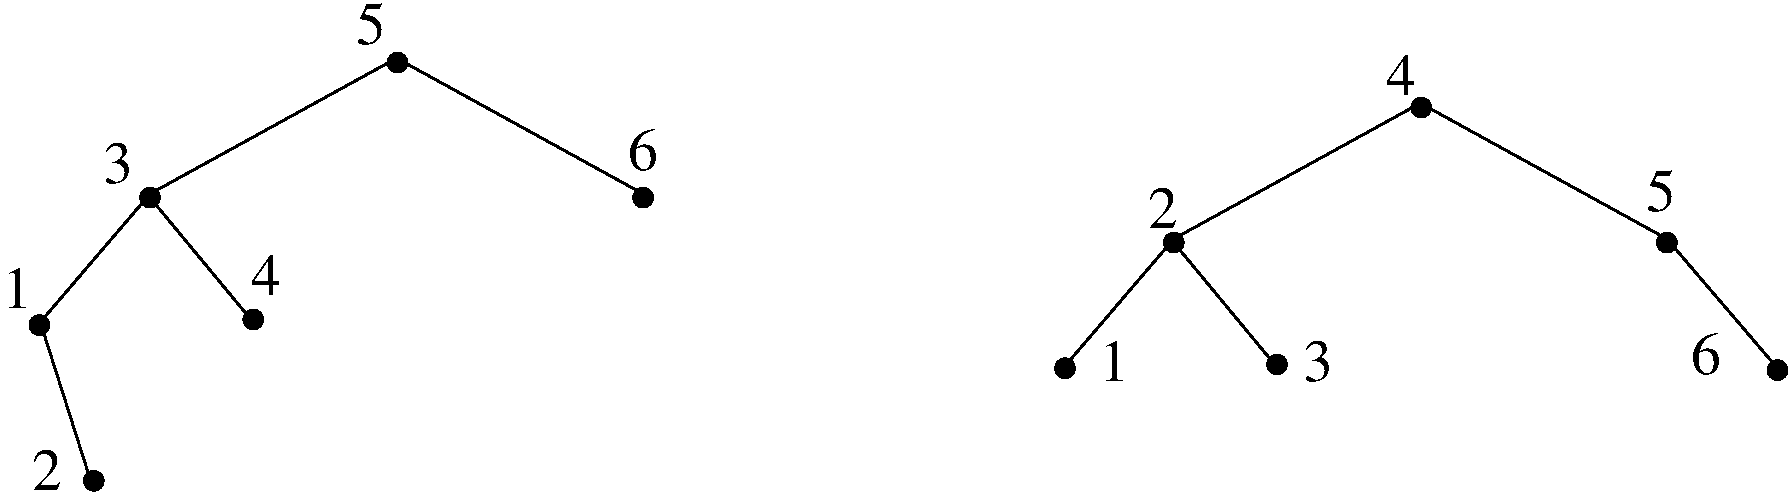
\includegraphics[width=0.6\linewidth,keepaspectratio]{balanced1}
\end{center}
\caption{Twee bomen met dezelfde knopen en verschillende hoogte \label{balanced1}}
\end{figure}


\subsection{Een meer compacte voorstelling voor bomen.}

% Bart: java aanpassing
Dikwijls wordt een boom voorgesteld met {\em gerichte} bogen; die
voorstelling benadrukt dat de functies {\em linkerkind} en {\em rechterkind}
dikwijls expliciet aanwezig zijn (in een Java-voorstelling van een
boom als velden in de klasse die de knoop voorstelt), doch niet
de functie {\em ouder}.

Daarenboven kan het ook nuttig zijn een boom als een (gerichte) graaf
voor te stellen die geen boom meer hoeft te zijn; neem bijvoorbeeld de
boomvoorstelling van de rekenkundige uitdrukking $(i+7)^{2} + i + 7$
in Figuur~\ref{boomexpressie}; daarin zie je twee deelbomen die
precies dezelfde zijn: de deelboom voor de deeluitdrukking $i+7$; de
overeenkomstige gerichte graaf (die geen boom meer is) staat in figuur
\ref{graafexpressie}. De voorstelling m.b.v. een gerichte graaf is
meer compact omdat  het voorkomen van de deeluitdrukking $i+7$ door
twee deelbomen {\em gedeeld} wordt (in het Engels: shared).

\begin{figure}[ht]
\mbox{
\hspace{0.5cm}
\subfigure[Boomvoorstelling]{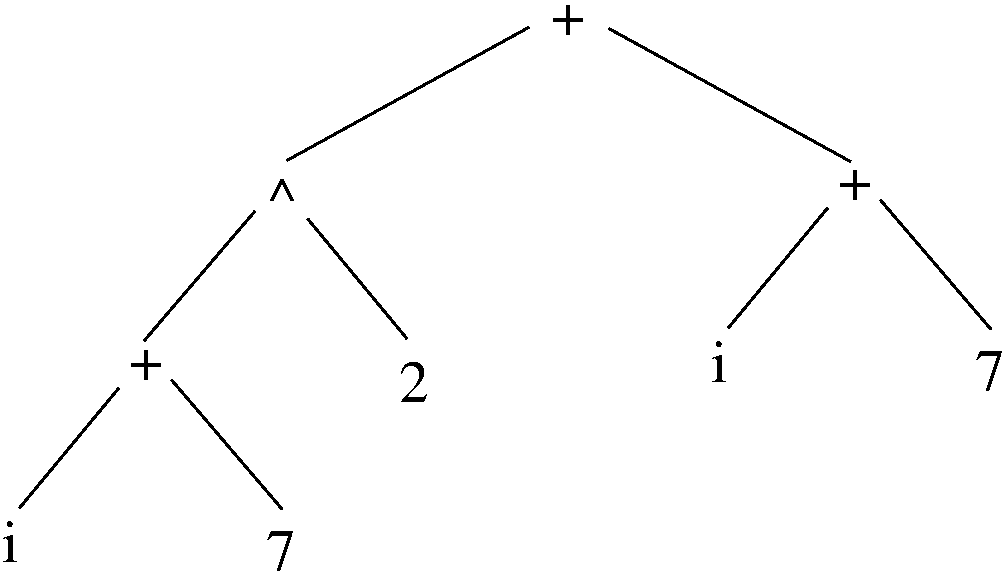
\includegraphics[width=0.4\linewidth,keepaspectratio]{boomexpressie} \label{boomexpressie}}\hspace{1cm}
\subfigure[Graafvoorstelling]{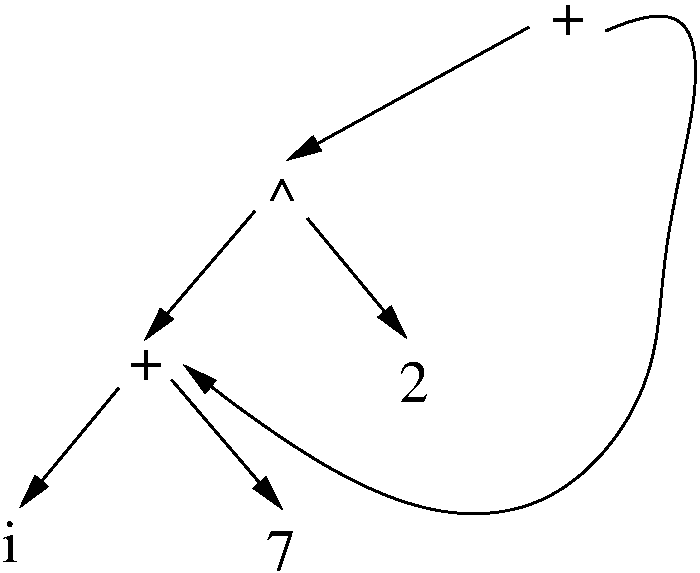
\includegraphics[width=0.3\linewidth,keepaspectratio]{grafeexpressie} \label{graafexpressie} }
}
\caption{Twee voorstellingen van $(i+7)^{2} + i + 7$}
\end{figure}

Het delen van deelbomen is niet zonder gevaar: als de gedeelde
deelboom gewijzigd wordt, veranderen beide voorkomens in de
niet-gedeelde voorstelling van de boom! Indien zulk een effect niet
gewenst wordt, mag men de effici\"entere voorstelling niet gebruiken.

\subsection{Opspannende bomen}

In deze sectie werken we uitsluitend met enkelvoudige grafen.

 \grijs{\begin{definitie} Opspannende boom\\
\textup{Een boom $T$ is een \textbf{opspannende boom} van een graaf $G$,
indien $T$ een subgraaf is van $G$ die alle knopen van $G$ bevat en $T$ een boom is.}
\end{definitie}}

Een opspannende boom draagt dus alle knopen van een graaf en is in
zekere zin een kleinste 
samenhangende
deelgraaf die alle knopen draagt: als je een
boog van een opspannende boom weglaat, dan zal je geen boom meer
hebben (de samenhangendheid verdwijnt) en misschien zal er een knoop niet meer
gedragen worden.

 \grijs{\begin{stelling}
Een graaf $G$ heeft een opspannende boom $T$ als en slechts als $G$ samenhangend is.
\end{stelling}}
\begin{proof}
\begin{itemize}
\item
Als $G$ een opspannende boom $T$ heeft, dan is $G$ samenhangend, want dan is
er een pad (over de bogen van de boom $T$) tussen elke twee knopen.

\item
Als $G$ samenhangend is en kringloos, dan is $G$ een boom en een
opspannende boom van zichzelf.

Indien $G$ samenhangend is en een kring heeft, verwijder dan \'{e}\'{e}n
boog uit die kring (maar geen knopen); de resulterende graaf is nog
steeds samenhangend en heeft een kring minder dan $G$; door inductie op
het aantal kringen is de stelling nu bewezen.
\end{itemize}
\end{proof}

De stelling doet meer dan het bestaan van een opspannende boom
bewijzen: het geeft een constructieve methode om een opspannende boom
te vinden; ruwweg: verwijder een boog uit elke kring en wat je
overhoudt is een opspannende boom. Een algoritme gebaseerd hierop is
niet erg effici\"ent, want het houdt in dat we kringen moeten zoeken en
dat is in het algemeen tijdrovend.

 \grijs{\begin{stelling} \label{opspannend4}
Karakterisatie van een opspannende boom\\
Een deelgraaf $T$ van een samenhangende graaf $G$ die kringvrij is en die
een maximaal aantal bogen van $G$ bevat, is een opspannende boom van $G$.
\end{stelling}}
\begin{proof}
We nemen aan dat $G$ minstens 2 knopen heeft.\\
Dat $T$ een maximaal aantal bogen bevat, betekent hier dat je geen boog kan
toevoegen zonder een kring te maken. We moeten bewijzen dat $T$
samenhangend is (dan is $T$ een boom) en dat $T$ alle knopen van $G$ bevat
(dan is $T$ opspannend).\\
Stel dat de knoop $v \in G \backslash T$; vermits $G$ samenhangend is 
bestaat er een boog $b$ die in $v$ toekomt; $b \notin T$ want anders zou
$v \in T$; vermits $T$ maximaal is, bevat de graaf $T \cup \{b\}$ 
een
kring die natuurlijk $b$ bevat. Maar dat betekent dat $v \in T$, hetgeen
in tegenspraak is met de onderstelling. Bijgevolg bevat $T$ alle knopen
van $G$.\\
Stel $T$ is niet samenhangend; beschouw de partitie in componenten
$\{T_{i}\}_{i=1}^{n}$. Figuur~\ref{opspannend3} laat $T_{1}$ en
$T_{2}$ zien. Vermits $G$ zelf samenhangend is, bestaan er knopen $v_{1}
\in T_{1}$ en $v_{2} \in T_{2}$ die verbonden zijn door een pad $P$
(zonder kring) in $G$ dat verder geen knopen met $T_{1}$ of $T_{2}$
gemeen heeft (op Figuur~\ref{opspannend3} in stippellijn). Onderstel
dat $P$ slechts \'{e}\'{e}n boog $b$ heeft. $T \cup \{b\}$ bevat nu een
kring en die kring loopt door $v_{1}$ en $v_{2}$; maar dat betekent
dat er al een pad was van $v_{1}$ naar $v_{2}$ in $T$, wat de
onderstelling dat $T_{1}$ en $T_{2}$ verschillende componenten waren
tegenspreekt.\\
We moeten nog bewijzen dat in een partitie $\{V_{k}\}_{k=1}^{n}$ van knopen
van een samenhangende graaf $G$, we altijd een $V_{i}$ en $V_{j}$ kunnen
kiezen zodanig dat er een $v_{i} \in V_{i}$ en $v_{j} \in V_{j}$ en de
boog $(v_{i},v_{j}) \in G$: neem $V_{1}$ en een willekeurige andere
$V_{k}$; daar G samenhangend is, bestaat er een pad van een knoop
$v_{1}$ naar een knoop van $V_{k}$; we kunnen $v_{1}$ zodanig kiezen
dat de eerste boog toekomt in een knoop $v \notin V_{1}$. Als $v \in
V_{k}$, dan zijn we klaar; anders behoort $v$ tot een $V_{j}$ met $j
\neq 1$ en we zijn klaar.
\end{proof}



Een bijkomende karakterisatie van opspannende bomen:

\begin{eig}
Indien $T$ een deelgraaf is van een samenhangende, enkelvoudige graaf $G$ met 
$n$
knopen, en $T$ is kringloos en heeft $n-1$ bogen, dan is $T$ een
opspannende boom van $G$.
\end{eig}

\begin{figure}[ht]
\begin{center}
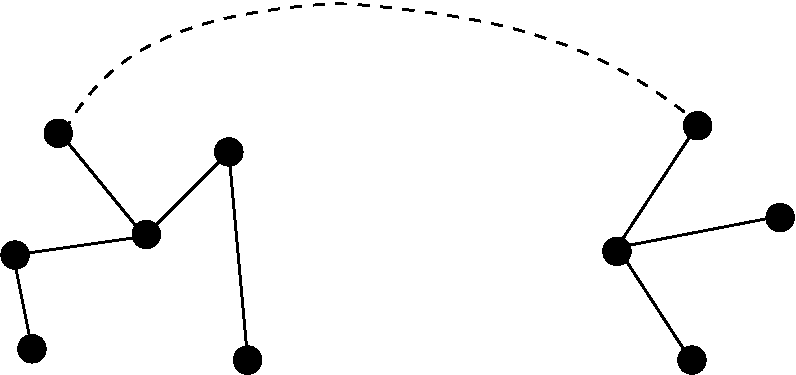
\includegraphics[width=0.3\linewidth,keepaspectratio]{opspannend3}
\end{center}
\caption{Twee componenten van $T$ verbonden door een pad van $G$
\label{opspannend3}}
\end{figure}

De Stelling~\ref{opspannend4} geeft aanleiding tot een algemeen
(niet deterministisch)
algoritme voor het construeren van een opspannende boom voor een graaf
$G$: vertrek van de lege graaf $T$; voeg aan $T$ herhaaldelijk een boog uit
$G$ toe die geen kring introduceert in $T$ en totdat dat niet meer
mogelijk is; $T$ is een opspannende boom.

Merk op dat: (1) je hoeft elke
boog maar \'{e}\'{e}n keer te beschouwen (waarom?) (2) de volgorde
waarin je bogen beschouwt, is onbelangrijk (3) uiteindelijk is $T$ een
boom, maar zolang je nog bezig bent met bogen toevoegen, hoeft $T$
niet samenhangend te zijn (4) je al kan stoppen als je $n-1$ bogen
hebt toegevoegd als $G$ $n$ knopen heeft.

Er zijn twee volgordes van bogen
kiezen die hun oorsprong vinden in algemene keuzestrategien (later ook
meer daarover in de sectie over het doorlopen van bomen): {\em
diepte-eerst} en {\em breedte-eerst}. We beschrijven de methodes
informeel:

\begin{description}
\item[Diepte-eerst constructie van opspannende boom:] kies een knoop
en construeer een zo lang mogelijk pad zonder kring vertrekkend van
die knoop; heel dat pad zal tot de opspannende boom behoren; keer
\'{e}\'{e}n stap terug in het pad en van daaruit construeer je weer
een zo lang mogelijk pad zonder kring - als dat niet ging, ga je nog
maar een stap terug; blijf dit doen tot je teruggekeerd bent in de
beginknoop en geen boog meer kan toevoegen; Figuur~\ref{diepteeerst1}
illustreert de methode, vertrekkend vanaf de topknoop: 
een boog behoort tot de opspannende boom indien hij getekend is in stippellijn.
\begin{figure}[ht]
\begin{center}
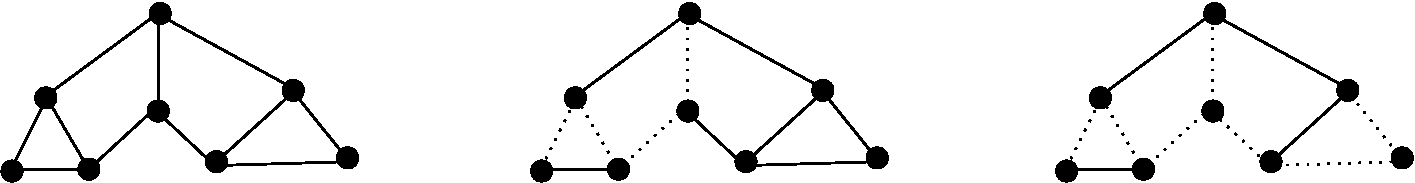
\includegraphics[width=0.6\linewidth,keepaspectratio]{diepteeerst1}
\end{center}
\caption{3 fazen in de diepte-eerst constructie van een opspannende boom \label{diepteeerst1}}
\end{figure}

\item[Breedte-eerst \ constructie \ van \ opspannende \ boom:] 
kies een knoop en 
neem alle bogen die daaruit vertrekken en zodanig
dat er geen kring gevormd wordt; al die bogen zullen behoren tot de
opspannende boom; in alle nieuwe knopen waar je met die net
toegevoegde bogen bent toegekomen, neem je weer alle bogen die
samengenomen met wat je al had, geen kring vormen; blijf dat doen tot
je geen bogen meer kan toevoegen; Figuur~\ref{breedteeerst1}
illustreert de methode, vertrekkend vanaf de topknoop.

\begin{figure}[ht]
\begin{center}
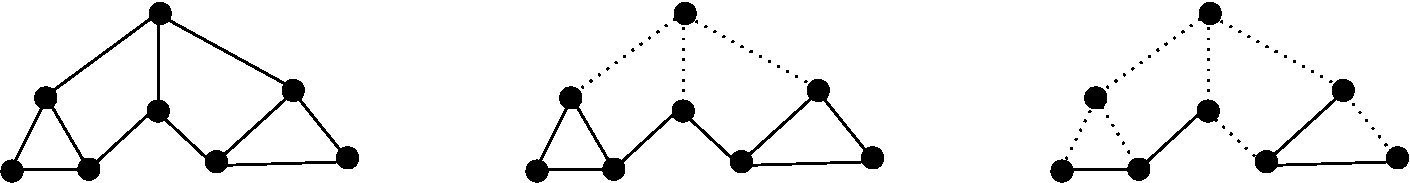
\includegraphics[width=0.6\linewidth,keepaspectratio]{breedteeerst1}
\end{center}
\caption{3 fazen in de breedte-eerst constructie van een opspannende boom \label{breedteeerst1}}
\end{figure}
\end{description}

De correctheid van beide methodes steunt op het feit dat alle bogen
ooit eens beschouwd worden als kandidaat voor toevoeging en stelling
\ref{opspannend4}. De orde is in beide methodes zo dat de
tussenliggende grafen altijd een boom zijn, want samenhangend.

Figuur~\ref{opspannend2} laat voor $K_{4}$ zien dat de diepte-eerst
opspannende bomen essentieel verschillen van de breedte-eerst
opspannende bomen.

\begin{figure}[ht]
\begin{center}
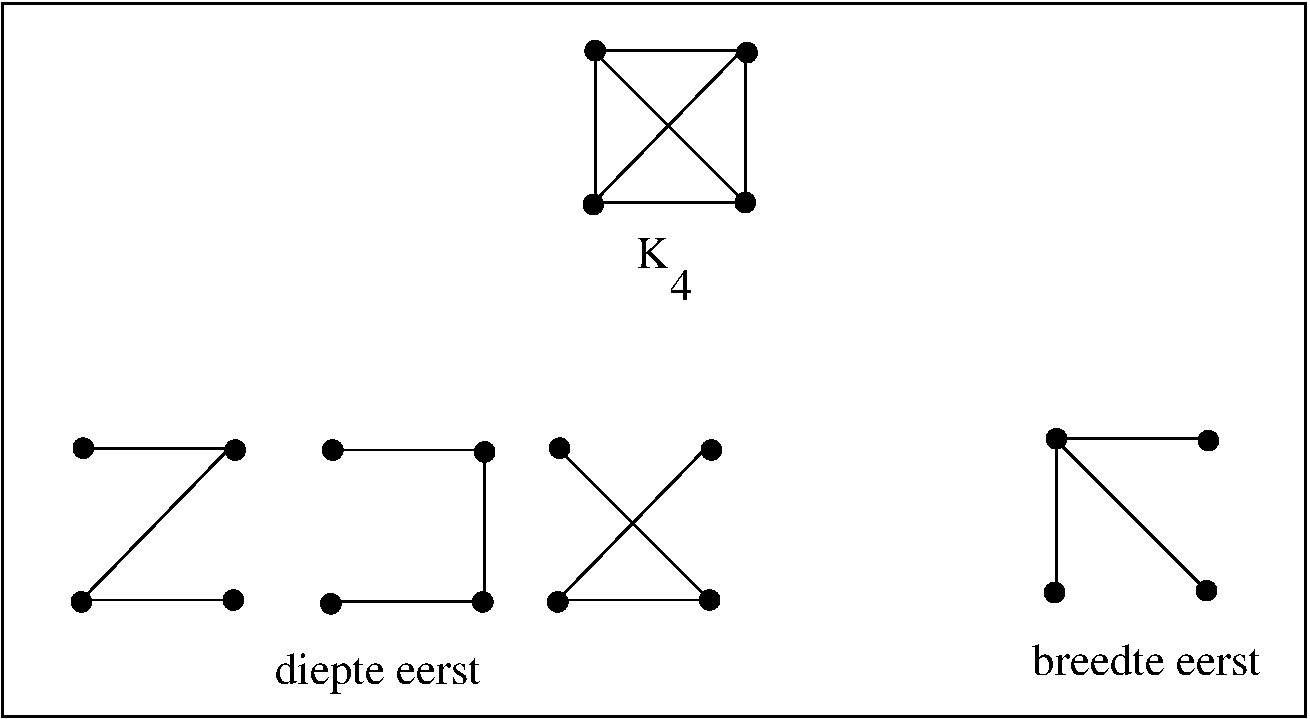
\includegraphics[width=0.5\linewidth,keepaspectratio]{opspannend2}
\end{center}
\caption{Opspannende bomen voor $K_{4}$\label{opspannend2}}
\end{figure}

Misschien heb je nu de indruk dat alle opspannende bomen kunnen
verkregen worden door ofwel de diepte-eerst ofwel de breedte-eerst
methode. Figuur~\ref{opspannend5} laat een graaf zien en een
opspannende boom, die met geen van beide methodes kan verkregen
worden.

\begin{figure}[ht]
\begin{center}
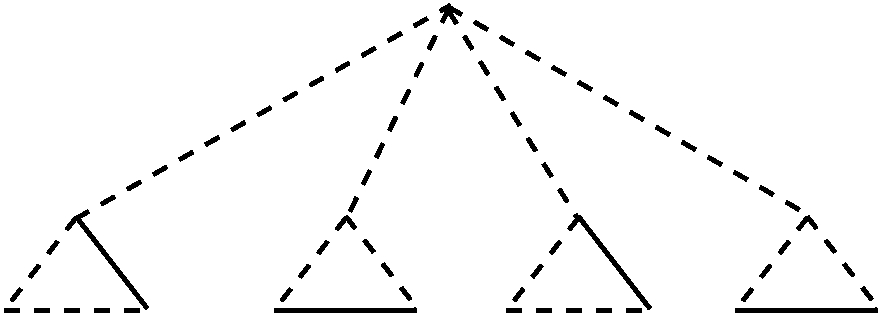
\includegraphics[width=0.5\linewidth,keepaspectratio]{opspannend5}
\end{center}
\caption{Graaf met een hybride opspannende boom\label{opspannend5}}
\end{figure}


\subsection{Minimale opspannende bomen}

Beschouwen we het volgende probleem: gegeven een aantal steden en stel
dat de kost van het bouwen van een weg tussen de steden gegeven is;
bepaal welke wegen moeten aangelegd worden om te voldoen aan (1) de
totale kost is minimaal (2) elke stad is bereikbaar vanuit elke andere
stad. Het wegennet dat daaraan voldoet moet een boom zijn, want er
kunnen geen kringen zijn (anders ware het net niet van minimale kost)
en er is een pad tussen elke twee steden. Dit soort bomen wordt
nu gedefinieerd:


 \grijs{\begin{definitie} Minimale opspannende boom\\
\textup{Voor een gewogen graaf $G$ is $T$ een \textbf{minimale opspannende
boom} indien $T$ een opspannende boom van $G$ is met het kleinste gewicht.}
\end{definitie}}

Figuur~\ref{opspannend1} laat een graaf $G$ zien, een opspannende boom $B$
en een minimale opspannende boom $T$.

\begin{figure}[ht]
\begin{center}
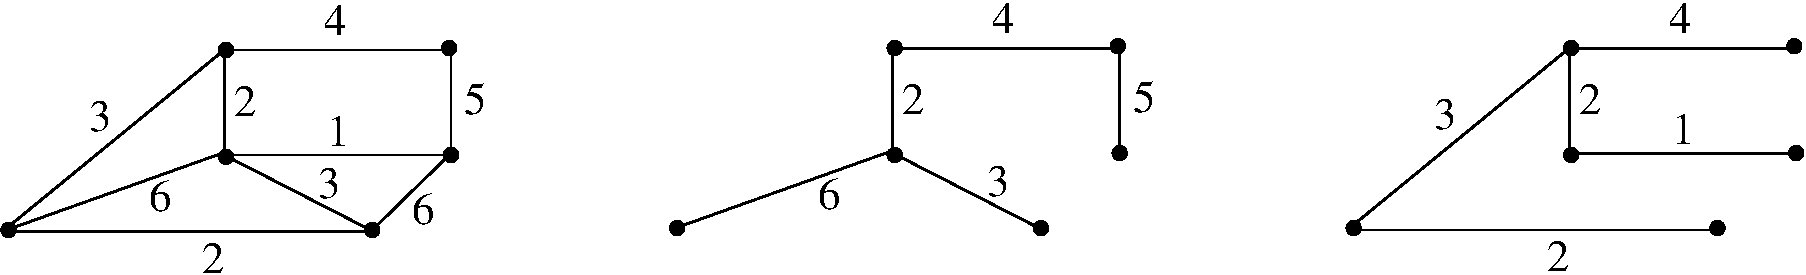
\includegraphics[width=0.6\linewidth,keepaspectratio]{opspannend1}
\end{center}
\caption{Een graaf met opspannende bomen\label{opspannend1}}
\end{figure}


Effici\"ente algoritmen die een minimale opspannende boom construeren
zijn gebaseerd op de volgende stelling:

 \grijs{\begin{stelling} Een boog die tot een minimale opspannende boom behoort \label{even}\\
  Gegeven een samenhangende graaf $(V,E)$, $U \subset V$ en $e$ een boog in $E$ met
  minimale lengte van alle bogen met begin in $U$ en einde in $V \backslash
  U$; er bestaat een minimale opspannende boom $T$ voor $(V,E)$ 
  zodanig dat $e \in T$.
\end{stelling}} % stelling 2.3 uit Shimon Even
\begin{proof} Neem een minimale opspannende boom $T_{0}$ voor de
graaf. Indien $e$ tot $T_{0}$ behoort is de stelling bewezen, indien
niet, voeg dan $e$ toe aan $T_{0}$. We verkrijgen $T_{1}$ die een kring
bevat (Stelling~\ref{opspannend4}) en die kring bevat $e$ alsook nog een 
boog $e' = (u,v)$
 waarbij $u \in U$ en $v \in V \backslash U$. Door uit $T_{1}$ $e'$ te
verwijderen verkrijgen we weer een opspannende boom $T$ (waarom is $T$ een
boom?) en bovendien is de 
$w(T) \leq w(T_{0})$ vermits $w(e)
\leq w(e')$. Bijgevolg is $T$ een minimale opspannende boom die $e$
bevat.
\end{proof}



\begin{algo} Prim \label{prim}\\
  Gegeven een samenhangende gewogen graaf $G(V,E)$ met een verzameling
  knopen $V =
  \{v_{1},v_{2},\ldots,v_{n}\}$.  De volgende procedure is een algoritme
  dat een minimale opspannende boom $T$ construeert.
\begin{enumerate}
\item \textbf{Initialisatie}: $T := (\{v_{1}\},\emptyset)$
\item \textbf{Stop?}: Indien $T$ $(n-1)$ bogen heeft, stop.
\item \textbf{Voeg boog toe}: 
Van alle bogen die een knoop van $T$ verbinden met een knoop die niet tot $T$
behoort, kies een boog $b$ met het kleinste gewicht en voeg
die toe aan $T$: er bestaat minstens \'{e}\'{e}n zulke boog omdat $G$
samenhangend is en $T$ nog niet alle knopen bevat; $T$ zal na
toevoeging van $b$ nog steeds kringloos zijn.
Ga naar \textbf{Stop?}.
\end{enumerate}
\end{algo}
\begin{proof} Vermits bij het einde van het algoritme $T$ een boom
is met $n$ knopen en $(n-1)$ bogen en $T$ kringloos is, is $T$ een opspannende
boom voor $G$. We moeten dus terminatie van het algoritme en
minimaliteit van $T$ bewijzen.

Een illustratie van de redenering hieronder, vind je in figuur
\ref{prim2}.

Eindigheid is eenvoudig want \textbf{Voeg boog toe} wordt slechts
$(n-1)$ keer uitgevoerd, waarna het algoritme stopt. Misschien wil je je
er nog van overtuigen dat \textbf{Voeg boog toe} altijd kan, t.t.z.
dat er altijd een boog bestaat die geen kringen introduceert in $T$.

Na \textbf{Initialisatie} bestaat $T$ uit \'{e}\'{e}n knoop en dus is $T$
een deel van een minimale opspannende boom (mob). We bewijzen nu dat
die eigenschap behouden blijft door \textbf{Voeg boog toe}: noteer met
W de knopen van $T$ en onderstel dat $T \subset T'$ met $T'$ een mob.
Noteer met $B = \{(x,y)\;|\; x \in W,\; y \in V \backslash W,\; (x,y) \in
E\}$.  Neem de kortste boog $(i,j)$ in $B$ die geen kring veroorzaakt
indien toegevoegd aan $T$. Indien $(i,j) \in T'$ dan is duidelijk dat $T
\cup \{(i,j)\} \subseteq T' = $mob. Indien $(i,j) \notin T'$ dan zal
$T' \cup \{(i,j)\}$ een kring bevatten, waarvan $(i,j)$ deel uitmaakt.
In die kring zit nog een boog $(x,y) \in B$ en door die uit $T' \cup
\{(i,j)\}$ te verwijderen krijgen we een nieuwe opspannende boom $T''$
(want bevat alle knopen en is samenhangend). De vraag is dan: is $T''$
ook minimaal? Vermits $w(i,j) \leq w(x,y)$ (zo was $(i,j)$ immers
gekozen), is $w(T'') \leq w(T')$ en bijgevolg is $T''$ een mob.
Bijgevolg is $T \cup \{(i,j)\}$ deel van een mob.

Bijgevolg is de opspannende boom door Prim geconstrueerd, een minimale
opspannende boom.
\end{proof}

\begin{figure}[ht]
\begin{center}
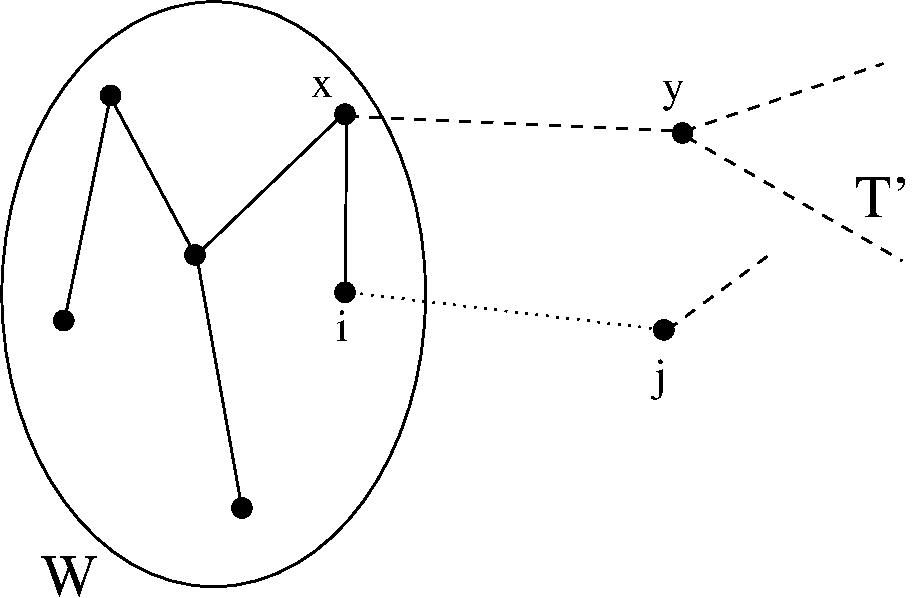
\includegraphics[width=0.4\linewidth,keepaspectratio]{prim2}
\end{center}
\caption{Illustratie bij Algoritme~\ref{prim} \label{prim2}}
\end{figure}


Het algoritme van Prim is een klassiek voorbeeld van een ``gulzig''
(Engels: greedy) algoritme: op elk ogenblik dat een keuze gemaakt moet
worden, wordt een keuze gemaakt die er op dat moment het beste uit
ziet, t.t.z.\ zonder te kijken naar de vorige keuzes (niet helemaal
correct) of naar de toekomstige keuzes. Niet elk gulzig algoritme
bereikt dan ook een optimaal resultaat; bv. een kortste-pad algoritme
dat op elk ogenblik een bestaand pad zou uitbreiden met de kortste
boog, geeft niet altijd een kortste pad en een gulzig schaakspeler
wint ook niet altijd. Doch in het geval van Prim werkt het perfect.

Het algoritme van Prim wordt ge\"{\i}llustreerd in Figuur~\ref{prim1}: de
initi\"ele knoop is A; de volgorde waarin de bogen worden toegevoegd,
staat bij de bogen als a,b,c \ldots h.

\begin{figure}[ht]
\begin{center}
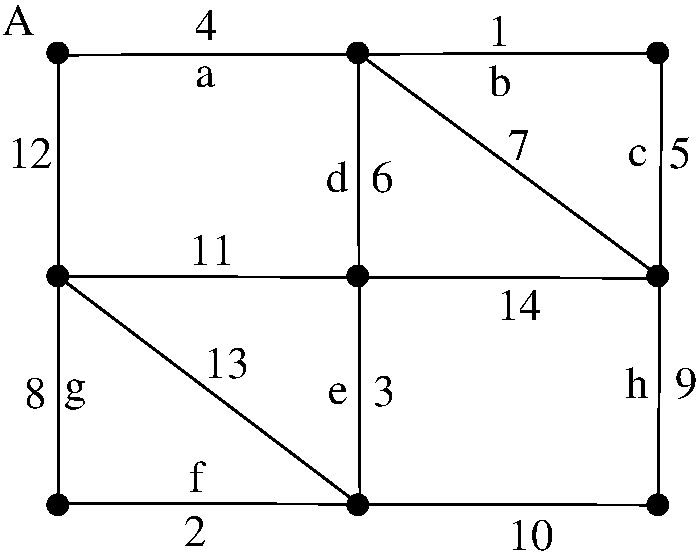
\includegraphics[width=0.3\linewidth,keepaspectratio]{prim1} % ,height=5cm}
\end{center}
\caption{De uitvoering van Algoritme~\ref{prim} \label{prim1}}
\end{figure}


Het algoritme van Prim bouwt een mob incrementeel, t.t.z. op elk
ogenblik in het algoritme is T een mob van een deelgraaf van G. Er is
een variante op het algoritme van Prim dat deze eigenschap niet heeft:

\newpage
\begin{algo} Kruskal \label{kruskal}\\
  Gegeven een samenhangende gewogen graaf G(V,E) met een verzameling
  knopen $V =
  \{v_{1},v_{2},\ldots,v_{n}\}$.  De volgende procedure is een algoritme
  dat een minimale opspannende boom $T$ construeert.
\begin{enumerate}
\item \textbf{Initialisatie}: $T := \emptyset$
\item \textbf{Stop?}: Indien $T$ $(n-1)$ bogen heeft, stop.
\item \textbf{Voeg boog toe}: Voeg aan $T$ toe een boog $b$ met minimaal
  gewicht en die bovendien geen kring veroorzaakt indien toegevoegd
  aan $T$. 
  Ga naar {\bf Stop?}.
\end{enumerate}
\end{algo}
\begin{proof}
Eindigheid van Kruskal is analoog aan die van Prim.
Dat $T$ op het einde een opspannende boom is, is ook analoog na te gaan.
We tonen nog de minimaliteit van $T$ aan.
%
Onderstel dat $T$ geen mob is.
Noem de bogen van $T$ $b_{1},b_{2},\ldots ,b_{n-1}$ in orde van toevoeging
door het algoritme.
Laat $S$ een mob (van $G$) zijn zodanig dat $\{b_{1}, b_{2}, \ldots ,
b_{i}\} \subseteq S$ en met maximale $i$ (zulk een S bestaat en door
Stelling~\ref{even} is $i \geq 1$!) Er zijn twee mogelijkheden:
\begin{itemize}
\item
\textbf{$i = n-1$}: nu is $T = S$ en $T$ is een mob.
\item
\textbf{$i < n-1$}: dus $b_{i+1} \notin S$; laat $H$ de graaf zijn
gevormd door de bogen $\{b_{1}, b_{2}, \ldots , b_{i}\}$ en hun
knopen. Beschouw de graaf $S \cup \{b_{i+1}\} = S'$. $S'$ heeft een
kring (want een boog te veel) waarin minstens \'{e}\'{e}n boog $b$ zit
die niet tot $T$ behoort (omdat $T$ zelf kringvrij is). Dus $b \in
S$. Nu bevat $H \cup \{b\}$ geen kring, want $H \cup \{b\} \subseteq
S$ en vermits Kruskal in de $(i+1)$-de \textbf{Voeg boog toe} de boog
$b_{i+1}$ koos (om toe te voegen aan $H$), moet $w(b_{i+1}) \leq
w(b)$. Bijgevolg is $S' \backslash \{b\} = S''$ een mob. Maar nu is $S''$
een mob die $\{b_{1}, b_{2}, \ldots , b_{i+1}\}$ omvat wat in
tegenspraak is met de maximaliteit van $S$. Dus het is niet mogelijk
dat $i < n-1$.
\end{itemize}
\end{proof}

Merk op dat $T$ tijdens Kruskal's algoritme geen boom hoeft te zijn: de
uitvoering van Kruskal wordt in Figuure~\ref{kruskal1}
ge\"{\i}llustreerd op dezelfde graaf als in Figuur~\ref{prim1}.

\begin{figure}[ht]
\begin{center}
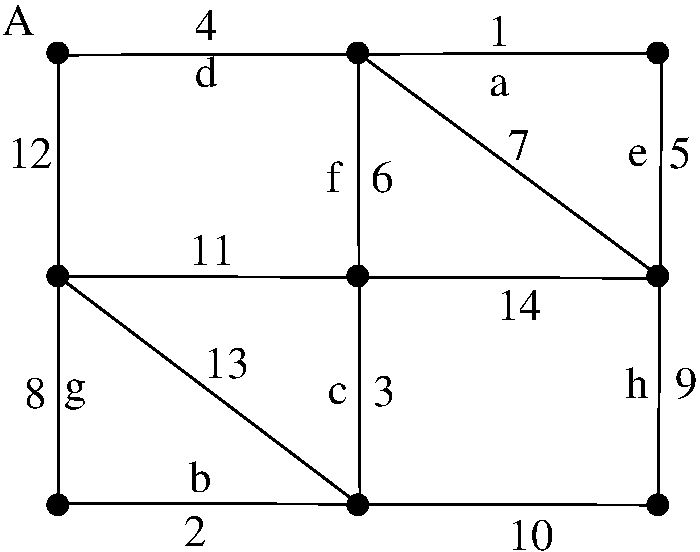
\includegraphics[width=0.3\linewidth,keepaspectratio]{kruskal1} % ,height=5cm}
\end{center}
\caption{De uitvoering van Algoritme~\ref{kruskal} \label{kruskal1}}
\end{figure}


\newpage
\section{Netwerkmodellen}

Een netwerk van verbindingen, elk met hun eigen capaciteit, kan
gemodelleerd worden als een gerichte, gewogen graaf. Als voorbeeld kan
je denken aan een wegennetwerk, een elektrisch netwerk of aan een stel
oliepijplijnen. Het belangrijkste probleem i.v.m. dit soort netwerken
is het optimaliseren van een stroming, zonder capaciteitsoverschreiding
natuurlijk. We zullen dit optimalisatieprobleem oplossen in de context
van grafentheorie. Ook andere problemen die op het eerste zicht niets
met optimalisatie van stroming te maken hebben, kunnen gemodelleerd
worden als een netwerkprobleem: personeelstoewijzing, toekenning van
resources en ook het partner-keuzeprobleem (``The marriage
problem''). 

\subsection{Transportnetwerk}

 \grijs{\begin{definitie} Transportnetwerk\\
{\rm Een \textbf{transportnetwerk} (of simpelweg een
\textbf{netwerk}) is een enkelvoudige, gewogen, gerichte graaf G die voldoet
aan
\begin{verse}
1. er is juist \'{e}\'{e}n knoop in G zonder binnenkomende bogen; deze
knoop wordt de \textbf{bron} genoemd

2. er is juist \'{e}\'{e}n knoop in G zonder buitengaande bogen; deze
knoop wordt de \textbf{put} genoemd (Engels: sink)

3.
het gewicht $C_{i,j}$ van de (gerichte) boog $(i,j)$ is postief en
wordt de \textbf{capaciteit} van de boog genoemd

4.
als de richting van de bogen vergeten wordt, dan is G samenhangend
\end{verse}
}
\end{definitie}}

Figuur~\ref{transport1} toont een netwerk: de bron is de knoop $a$ en de
put is de knoop $z$; de capaciteit van elke boog is bij de boog
geschreven. Het netwerk modelleert bijvoorbeeld een stel
eenrichtingsstraten in een stad tussen het station (knoop $a$) en de
markt (knoop $z$); de capaciteit is het aantal voertuigen dat per minuut
kan passeren door elke straat.

\begin{figure}[ht]
\begin{center}
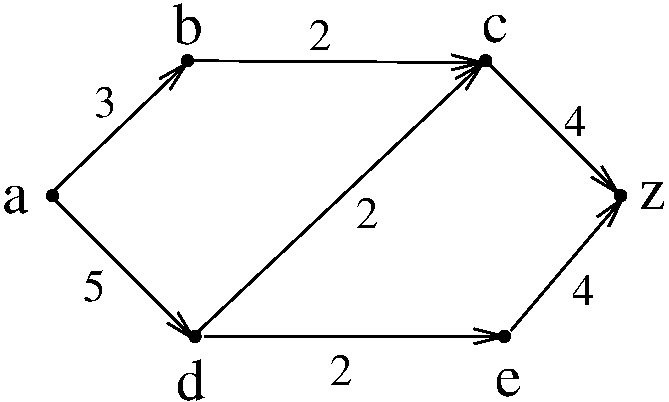
\includegraphics[width=0.3\linewidth,keepaspectratio]{transport1} % ,height=3cm}
\end{center}
\caption{Een transportnetwerk \label{transport1}}
\end{figure}

De beperking dat een netwerk enkelvoudig moet zijn, is niet erg groot:
zowel lussen als parallelle bogen kan je wegwerken door knopen bij te
zetten op elke lus of parallelle boog; er verandert niets essentieels
aan het netwerk wat betreft de problemen die we bestuderen in deze
sectie.

 \grijs{\begin{definitie}Stroming in een netwerk \label{stroming1}
\label{stromingdef}\\
{\rm Voor een netwerk $G(V,E)$ met capaciteit $C_{i,j},\;\; i,j \in
    V$\footnotemark
    is $F$ een \textbf{stroming} als $F$ een afbeelding is
    van $E$ naar $\R^{+}$ zodanig dat\\
\begin{minipage}{12cm}
\begin{enumerate}
\item
\label{stromingdef1}
$F(i,j) \leq C_{i,j}$
\item \label{conserve1} voor elke knoop $j$ die niet de bron of de put is geldt:
\[\displaystyle \sum_{i \in V} F(i,j) = \sum_{i \in V} F(j,i)\]
\end{enumerate}
\end{minipage}\\[2mm]
We noemen $F(i,j)$ de stroming in boog $(i,j)$. Voor een knoop $j$ noemen we
$\sum_{i \in V} F(i,j)$ de stroming \textbf{naar} of \textbf{in} $j$ en
$\sum_{i \in V} F(j,i)$ de stroming \textbf{uit} $j$.
}
\end{definitie}}
\footnotetext{als er geen 
boog $(i,j)$ bestaat, dan nemen we aan dat $C_{i,j} = 0$} 

Formule~\ref{conserve1} in Definitie~\ref{stroming1} drukt het behoud
van stroming uit: alles wat binnenkomt in een knoop, gaat er weer buiten
en alles wat buitengaat, is binnengekomen; dat verhindert dat er een
ophoping of productie gebeurt in de knopen.

Figuur~\ref{stroom2} toont een stroming voor het netwerk van figuur
\ref{transport1}; de stroming is gedefinieerd door:
\begin{center}
$
\begin{array}{l}
F(a,b) = 2\\
F(b,c) = 2\\
F(c,z) = 3\\
F(a,d) = 3\\
F(d,c) = 1\\
F(d,e) = 2\\
F(e,z) = 2\\
\end{array}
$
\end{center}
en telkens naast de capaciteit van de overeenkomstige boog gezet.
\begin{figure}[ht]
\begin{center}
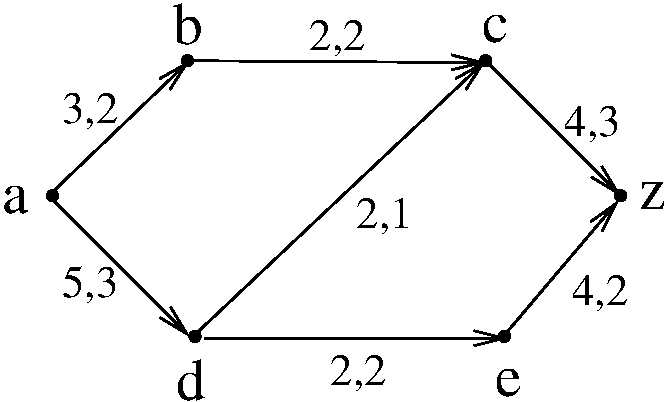
\includegraphics[width=0.3\linewidth,keepaspectratio]{stroom2} % ,height=3cm}
\end{center}
\caption{Een stroming in een transportnetwerk \label{stroom2}}
\end{figure}

Je kan nagaan dat Formule~\ref{conserve1} in Definitie~\ref{stroming1}
voldaan is voor elke knoop behalve de bron en de put.

Je kan ook nagaan dat de stroming uit de bron gelijk is aan de stroming in
de put:
\begin{center}
\mbox{$F(a,b)+F(a,d) = F(c,z) + F(e,z)$}.
\end{center}
Deze gelijkheid wordt veralgemeend in:

 \grijs{\begin{stelling} Bron-uit = put-in \label{bron=put}\\
Van een stroming $F$ in een netwerk $G(V,E)$ is de stroming uit de bron gelijk
aan de stroming in de put, of meer formeel: 
\[\sum_{i \in V} F(a,i) =
\sum_{i \in V} F(i,z).\]
\end{stelling}}
\begin{proof}

Het is duidelijk dat

$~~~~~~~~~~\sum_{j \in V} (\sum_{i \in V} F(i,j))  = 
                \sum_{i \in V} (\sum_{j \in V} F(i,j))
         =  \sum_{j \in V} (\sum_{i \in V} F(j,i))$


De omwisseling van de $\sum$'s mag omdat we met eindige grafen te
doen hebben. De tweede gelijkheid geldt wegens hernoeming van $i$ en $j$.

Daaruit volgt:

\begin{tabular}{c c c l}
~~~~~~~~~ &
0 & = & $\sum_{j \in V} \left(\sum_{i \in V} F(i,j) - \sum_{i \in V} F(j,i) \right)$\\
 & & & \\
 &  & = & $\left( \sum_{i \in V} F(i,z) -  \sum_{i \in V} F(z,i)\right) +
                \left(\sum_{i \in V} F(i,a) -  \sum_{i \in V} F(a,i)\right)$
    \\
 & & & \\
 &  &  & \hspace*{2cm}
       $+ \sum_{j \in V \backslash \{a,z\}} \left( \sum_{i \in V} F(i,j) -
                \sum_{i \in V} F(j,i)\right)$\\
 & & & \\
 & & = & $\sum_{i \in V} F(i,z) - \sum_{i \in V} F(a,i)$
\end{tabular}



vermits $F(z,i) = 0 = F(i,a)$ voor $\forall i \in V$ (door Definitie~\ref{stromingdef})

en $\sum_{i \in V} F(i,j) = \sum_{i \in V} F(j,i)$ voor $\forall j \in (V \backslash \{a,z\})$ (door Formule~\ref{conserve1} in Definitie~\ref{stromingdef})
\end{proof}



Op basis van Stelling~\ref{bron=put}, kunnen we nu defini\"eren:

 \grijs{\begin{definitie} Grootte van een stroming\\
\textup{De \textbf{grootte van een stroming $F$} in een netwerk $G(V,E)$
met bron $a$ en put $z$ is gedefinieerd door $\sum_{i \in V} F(a,i)$ of
$\sum_{i \in V} F(i,z)$ }
\end{definitie}}

De grootte van de stroming in Figuur~\ref{stroom2} is 5.



Het netwerkprobleem kan nu als volgt geformuleerd worden: voor een
gegeven netwerk $G$, vind de maximale stroming, of m.a.w. vind de stroming
met de maximale grootte.



Tot slot van deze sectie, nog iets over netwerken met meer dan
\'{e}\'{e}n bron of put: het netwerk in Figuur~\ref{transport2} stelt
de waterbevoorrading van de steden $A$ en $B$ voor, vanuit de bronnen $X,Y$
en $Z$ en over verdeelstations $b,c$ en $d$.

\begin{figure}[ht]
\begin{center}
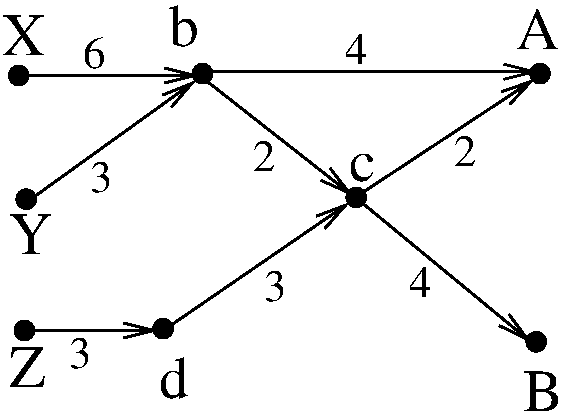
\includegraphics[width=0.22\linewidth,keepaspectratio]{transport2} % ,height=3cm}
\end{center}
\caption{Een transportnetwerk met meerdere bronnen en putten \label{transport2}}
\end{figure}

Door een superbron $a$ en een superput $z$ toe te voegen aan dit netwerk,
verkrijgen we terug een gewoon netwerk: vanuit $a$ voeg je ook een
gerichte boog toe naar elke bron van het originele netwerk, en vanuit
elke oude put een gerichte boog naar $z$; de toegevoegde bogen krijgen
alle de capaciteit $\infty$.

\begin{figure}[ht]
\begin{center}
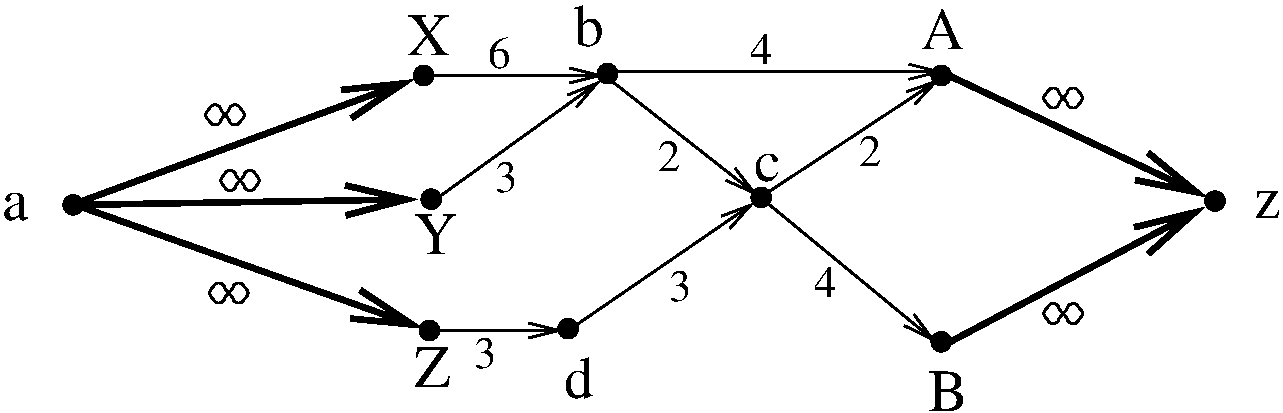
\includegraphics[width=0.507\linewidth,keepaspectratio]{transport3} % ,height=3cm}
\end{center}
\caption{Een transportnetwerk met een superbron en superput \label{transport3}}
\end{figure}

In dit nieuwe netwerk geeft een maximale stroming ook een maximale
stroming voor het oorspronkelijke netwerk.

Denk niet dat een maximale stroming uniek is: Figuur~\ref{stroom3} toont
een netwerk met oneindig veel maximale stromen, nl. voor alle i,j die
voldoen aan $i+j = 5$ en $0 \leq i,j \leq 3$.

\begin{figure}[ht]
\begin{center}
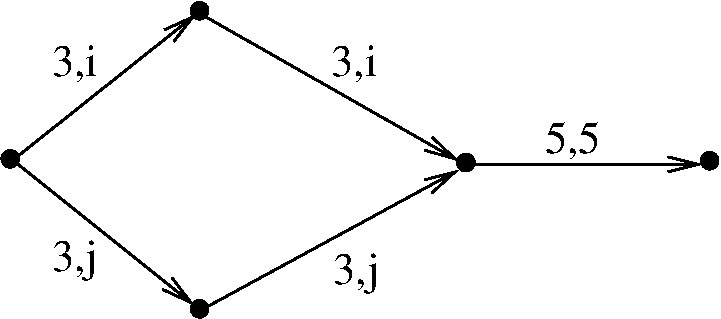
\includegraphics[width=0.3\linewidth,keepaspectratio]{stroom3} % ,height=2.5cm}
\end{center}
\caption{Een netwerk met oneindig veel maximale stromen\label{stroom3}}
\end{figure}


\subsection{Maximale stroming}

We zullen een algoritme zien om een maximale stroming te berekenen; 
het basisidee is eenvoudig: vertrek van een stroming en verbeter die totdat
dat niet meer mogelijk is; je hebt nu een maximale stroming. Een
intu\"{\i}tieve beschrijving van hoe je een stroming verbetert, gaat als
volgt:
\begin{itemize}
\item
neem een pad $P$ van de bron $a$ naar de put $z$
\item
zoek het minimum $\Delta$ van $C_{b} - F(b)$ over alle bogen $b \in P$
\item
bepaal de nieuwe stroming langs het pad $P$ door bij elke $F(b)$ $\Delta$ 
bij te tellen
\end{itemize}

Een paar opmerkingen bij dit voorschrift:
\begin{itemize}
\item de operatie verhoogt de stroming enkel als het pad $P$ (toevallig)
  zo is dat $\Delta > 0$
\item de beschrijving geldt alleen voor een pad waarvan elke boog de
goede richting heeft, maar
\item we mogen niet alleen paden van $a$ naar $z$ zoeken langs de
gerichte bogen: bekijk Figuur~\ref{transport4}; daarin zie je dat geen
enkel pad van $a$ naar $z$ met enkel goede bogen ``verbeterd'' kan
worden met bovenstaande methode; maar de stroming langs het pad
$(a,b,c,z)$ kan wel verbeterd worden door de stroming getoond in
Figuur~\ref{transport5};

\begin{figure}[ht]
\begin{center}
\subfigure[Een niet maximale stroming]{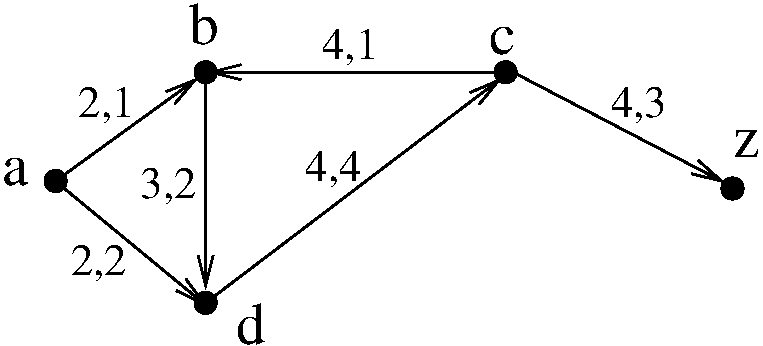
\includegraphics[width=0.3\linewidth,keepaspectratio]{transport4} \label{transport4}}\hspace{1.2cm}
\subfigure[Een verbeterde stroming langs een pad met omgekeerde boog]{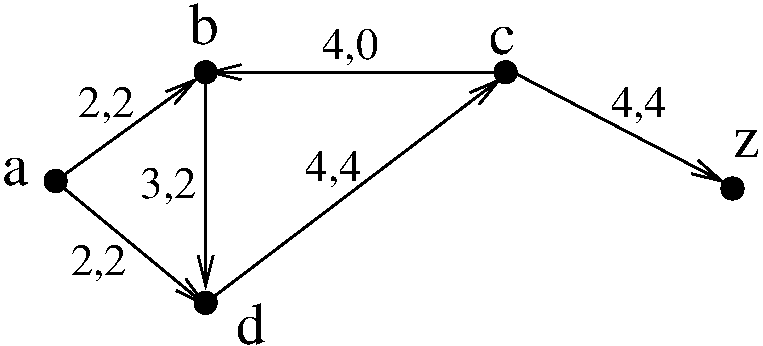
\includegraphics[width=0.3\linewidth,keepaspectratio]{transport5} \label{transport5}}
\end{center}
\caption{Verbetering van stroming}
\end{figure}

we moeten dus ook paden beschouwen waarvan bogen ``omgekeerd'' lopen
en we moeten voor die verkeerde bogen niet iets optellen bij de
stroming, maar er iets aftrekken: als een ``omgekeerde'' boog een stroming
draagt kan het immers zijn dat er alleen maar iets rondstroomt zonder
ooit de put te bereiken; we formaliseren dat als volgt:
\end{itemize}

 \grijs{\begin{definitie} Goede en slechte boog\\
\textup{In een gerichte graaf $G(V,E)$ met pad $(v_{1},v_{2},\ldots ,v_{n})$
noemen we de boog $(v_{i},v_{i+1})$ \textbf{goed} (gericht) indien
$(v_{i},v_{i+1}) \in E$ en anders \textbf{slecht} (gericht)}
\end{definitie}}

In een pad $P$ zullen we de goede bogen noteren door $P_{+}$ en de
slechte door $P_{-}$.


 \grijs{\begin{stelling} Verbeteren van een stroming
\label{verbeterstroming}\\
Laat $P$ een pad zijn van $a$ naar $z$ in een netwerk $G(V,E)$, waarbij
\begin{verse}
1.
$\forall (i,j) \in P_{+}$: $F(i,j) < C_{i,j}$

2. 
$\forall (i,j) \in P_{-}$: $0 < F(i,j)$
\end{verse}

Laat bovendien $\Delta = min(min_{(i,j) \in P_{+}}
\{C_{i,j}-F(i,j)\},min_{(i,j) \in P_{-}} \{F(i,j)\})$; definieer de
functie $F'$ als volgt:

\begin{eqnarray*}
F'(i,j) & = & F(i,j) \quad \forall (i,j) \notin P\\
        & = & F(i,j) + \Delta \quad \forall (i,j) \in P_{+}\\
        & = & F(i,j) - \Delta \quad \forall (i,j) \in P_{-}
\end{eqnarray*}

Dan is $F'$ een stroming waarvan de grootte $\Delta$ meer is dan die van $F$.

\end{stelling}}
\begin{proof} Om na te gaan dat $F'$ een stroming is, moeten we
\ref{stromingdef1} en~\ref{conserve1} van Definitie~\ref{stromingdef}
bewijzen: beide zijn niet moeilijk.

Dat de stroming met $\Delta$ verbeterd is, volgt uit het feit dat de
stroming van de boog $(a,\_) \in P$ (en die is goed - waarom?) met
$\Delta$ is verhoogd en de stroming door de andere bogen die vertrekken
in $a$ niet is veranderd.  \end{proof}



E\'{e}n van de gevolgen van de stelling over de verbetering van de
stroming, is dat bij een maximale stroming $F$ elk pad van $a$ naar $z$,
minstens \'{e}\'{e}n goede boog heeft met $C_{i,j} = F(i,j)$ of
\'{e}\'{e}n slechte boog met $F(i,j) = 0$; zoniet kon de stroming
verbeterd worden langs dat pad.

We zouden ook graag de volgende eigenschappen hebben:
\begin{itemize}
\item
als een stroming geen enkel pad van $a$ naar $z$ heeft dat kan verbeterd
worden (volgens de methode van Stelling~\ref{verbeterstroming}) dan is
de stroming maximaal - dit lijkt voor de hand liggend, maar is niet
triviaal te bewijzen!
\item
een algoritme om de flow te maximaliseren bestaat erin om
een pad te zoeken dat aan de voorwaarden van stelling
\ref{verbeterstroming} voldoet, de stroming langs het pad te verbeteren en
dat te herhalen tot er geen zulk pad meer is - indien voorgaand
puntje waar is en de procedure eindigt, dan levert dit inderdaad een
maximale stroming op.
\end{itemize}

We zullen beide eigenschappen formeel aantonen. We beschrijven eerst
een klassiek algoritme dat een voorbeeld is van een ``labeling
procedure''. Je hebt vroeger al een algoritme gezien dat labels
gebruikte nl. het kortste-pad algoritme van Edgser Dijkstra: knopen kregen
daarbij een label met informatie. In het volgende algoritme gebruiken
we een dubbel label: informeel is de eerste component van
het label de knoop waarvan je kwam (en daarom zal de startknoop een
lege eerste component in zijn label hebben) en de tweede component van
het label zal de $\Delta$ uit Stelling~\ref{verbeterstroming} zijn van
het pad dat tot dan is gevonden.

\begin{algo} Constructie van een maximale stroming.
\label{maxflow}\\
Laat $G(V,E)$ een netwerk zijn met bron $a$ en put $z$ en capaciteit $C$,
waarbij alle capaciteiten positief en geheel zijn. Onderstel een
orde op de knopen met $a = v_{0}, v_{1}, \ldots , v_{n} = z$.

Met ${\cal B}$ zullen we de verzameling beschouwde knopen aanduiden;
met ${\cal L}$ de verzameling van knopen met een label; de operaties
op ${\cal B}$ zullen we expliciet maken; die op ${\cal L}$ zijn impliciet.

\begin{enumerate} \item \textbf{Initialisatie}:
Definieer $\forall (i,j) \in E: F(i,j) = 0$

\item
\textbf{Label de bron}: Geef $a$ het label $(\_,\infty)$;  zet ${\cal B} = \emptyset$

\item
\textbf{Aangekomen?}: Indien $z$ een label heeft, verbeter de stroming
en ga terug naar \textbf{Label de bron}.

Verbeter de stroming gaat als volgt: er is juist \'{e}\'{e}n pad $P$ van $a$ naar
$z$ dat achteruit kan geconstrueerd worden te vertrekken van $z$, dan
de eerste component van het label van $z$ en zo verder tot in $a$. De
tweede component van het label van $z$ is een grootheid $\Delta$ die
nu wordt bijgeteld bij $F$ voor goede bogen in $P$ en afgetrokken van
$F$ voor slechte bogen van $P$. Daarna worden alle labels in heel het
netwerk gewist.

\item
\textbf{Kies volgende knoop}: Indien ${\cal L} \setminus {\cal B} =
\emptyset$, \textbf{stop}: de stroming $F$ is maximaal.

Noem $v$ de nog niet beschouwde knoop $v_{i}$ met een label en met
kleinste index $i$.
\item
\textbf{Label buren}: Stel dat het label van $v$ gelijk is aan
$(\alpha,\Delta)$. Behandel nu elke boog van de vorm $(v,w)$ of
$(w,v)$ in de volgorde $(v,v_{0})$, $(v_{0},v)$, $(v,v_{1})$, $(v_{1},v)$,
$\ldots $ waarbij $w$ nog geen label heeft.
\begin{itemize}
\item
voor elke boog $(v,w)$ (dus een boog die wegloopt uit $v$):
indien $F(v,w) < C_{v,w}$ geef $w$ het label $(v,min\{\Delta,C_{v,w}-F(v,w)\})$
anders geef je $w$ geen label
\item
voor elke boog $(w,v)$ (dus een boog die toekomt in $v$):
indien $F(w,v) > 0$ geef $w$ het label $(v,min\{\Delta,F(w,v)\})$
anders geef je $w$ geen label
\end{itemize}
Ga naar \textbf{Aangekomen?}
\end{enumerate}
\end{algo}
\begin{proof}
~\\
\begin{itemize}
\item
\textbf{Eindigheid}:
Punt 3 in het algoritme is cruciaal: zolang de uitgang \textbf{stop}
niet genomen wordt, wordt punt 3 herhaaldelijk uitgevoerd. Vanuit punt
3, gaat de uitvoering ofwel naar punt 2 of punt 4. De overgang van
punt 3 naar punt 2 kan maar een eindig aantal keer gebeuren, want die
overgang impliceert dat de stroming verbeterd wordt met $\Delta > 0$;
$\Delta$ is geheel omdat alle capaciteiten geheel zijn en vermits de
maximale stroming begrensd is (door de som van de capaciteiten van de
bogen die vertrekken in de bron) kan de gegeven stroming dus slechts
een eindig aantal keer verbeterd worden. Na een eindig aantal
overgangen van punt 3 naar punt 2, wordt dus steeds opnieuw de
overgang van punt 3 naar punt 4 genomen. In punt 4 wordt telkens een
knoop toegevoegd aan ${\cal B}$ (die nooit meer terug op $\emptyset$
wordt gezet). Bijgevolg zal na verloop van tijd ${\cal L}={\cal B}$ en
op dat moment stopt het algoritme.
\item
\textbf{Maximaliteit}: we stellen het bewijs nog even uit tot we
Stelling~\ref{maxflowmincut} hebben gezien.
\end{itemize}
\end{proof}

Merk op dat het Algoritme~\ref{maxflow} niet alle maximale stromen
vindt: zie Figuur~\ref{stroom3}.


 \grijs{\begin{definitie} Snede van een netwerk\\
  \textup{Een \textbf{snede} van een netwerk $G(V,E)$ met bron $a$ en put
    $z$, is een 2-tal $(P,\overline{P})$ 
    zodanig dat $a \in P$, $z \in \overline{P}$, $P
    \cup \overline{P} = V$ en $P \cap \overline{P} = \emptyset$ }
\end{definitie}}

We kunnen een snede tekenen door een lijn die de knopen van het
netwerk in twee verzamelingen verdeelt: op Figuur~\ref{snede1} is een
snede aangegeven met een stippellijn.

\begin{figure}[ht]
\begin{center}
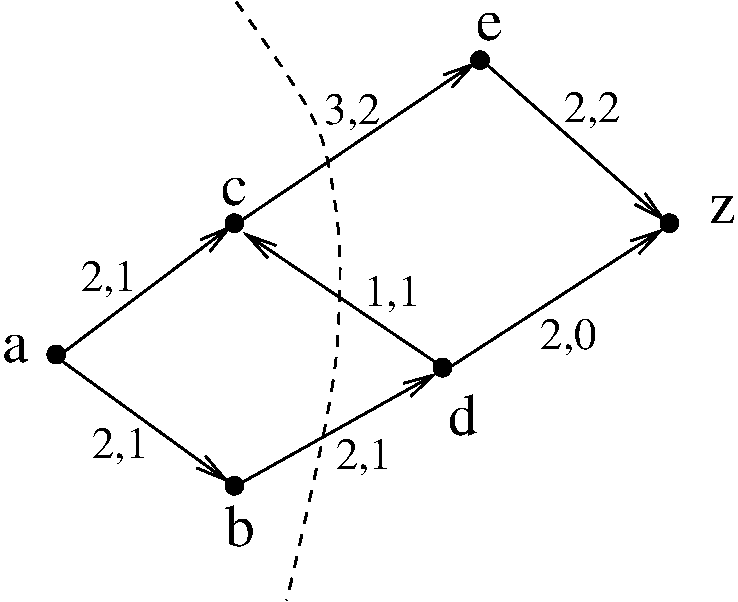
\includegraphics[width=0.3\linewidth,keepaspectratio]{snede1} % ,height=4cm}
\end{center}
\caption{Een netwerk met een stroming en een snede\label{snede1}}
\end{figure}

We kunnen nagaan hoeveel stroming er globaal loopt over de snede,
t.t.z. van links naar rechts in de tekening van een netwerk: daarbij
moeten we een boog van P naar $\overline{P}$ positief rekenen en een
omgekeerde boog negatief; voor het net in Figuur~\ref{snede1} wordt
dat: \mbox{$~~~~~~~~F(c,e) + F(b,d) - F(d,c) = 2+1-1=2$ }

Vergelijken we die grootheid met de stroming (in {\em a} of {\em z}) dan zien we
dat die ook gelijk is aan 2! Is dit toeval of niet? We kunnen ook
proberen een afschatting te maken van hoeveel stroming er maximaal van
links naar rechts over de snede kan lopen, door optimistisch te
veronderstellen dat er misschien een stroming bestaat die voor alle
goede bogen over de snede maximaal is, t.t.z. gelijk aan de capaciteit
van die boog en voor alle slechte bogen nul. We zullen die grootheid
de capaciteit van de snede noemen. Voor hetzelfde voorbeeld geeft dat: 
\mbox{$~~~~~~~~C_{c,e} + C_{b,d} = 2+3=5$}

En het lijkt alsof capaciteit van de snede groter is dan de stroming
van de snede en ook groter dan de maximale stroming (je kan nagaan dat
die 4 is). Is dit toeval? We bekijken deze vragen in een meer
formeel kader:

 \grijs{\begin{definitie} Capaciteit $C(P,\overline{P})$ van een snede\\
  \textup{De \textbf{capaciteit van een snede} $(P,\overline{P})$ is
    $C(P,\overline{P}) = \displaystyle
    \sum_{i \in P} \sum_{j \in \overline{P}} C_{i,j}$}
\end{definitie}}

 \grijs{\begin{stelling} \label{snedestroming}
De capaciteit van een snede is niet kleiner dan een stroming, m.a.w.
\[\sum_{i \in P} \sum_{j \in \overline{P}} C_{i,j} \geq \sum_{i \in V} F(a,i).\]
\end{stelling}}
\begin{proof}
\begin{eqnarray*}
\sum_{i \in V} F(a,i) & = & 
                \sum_{i \in V}(F(a,i) - F(i,a)) +
                \sum_{j \in P \backslash \{a\}} \sum_{i \in V}(F(j,i) - F(i,j))\\
        & = & \sum_{j \in P} \sum_{i \in V} (F(j,i) - F(i,j)) \\
        & = & \sum_{j \in P} \sum_{i \in P} F(j,i) +
                \sum_{j \in P} \sum_{i \in \overline{P}} F(j,i) -
                \sum_{j \in P} \sum_{i \in P} F(i,j) -
                \sum_{j \in P} \sum_{i \in \overline{P}} F(i,j)\\
        & = & \sum_{j \in P} \sum_{i \in \overline{P}} F(j,i) -
                \sum_{j \in P} \sum_{i \in \overline{P}} F(i,j)\\
        & \leq & \sum_{j \in P} \sum_{i \in \overline{P}} F(j,i)\\
        & \leq & C(P,\overline{P})
\end{eqnarray*}
\end{proof}

Merk op dat de derde laatste regel van de stelling inderdaad aantoont
dat de stroming gelijk is aan de stroming die door de snede loopt.



Een \textbf{minimale} snede is een snede met minimale capaciteit.
Vorige stelling impliceert direct dat de maximale stroming kleiner of
gelijk is aan de capaciteit van de minimale snede. Het verband tussen
beide grootheden is nog sterker:


 \grijs{\begin{stelling} Max flow - min cut \label{maxflowmincut}\\
  Voor een snede $(P,\overline{P})$ en stroming $F$ in een net $G(V,E)$ 
  geldt dat als 
\[C(P,\overline{P})=F\mbox{ \ \ (of dus als }
\sum_{i \in P} \sum_{j \in \overline{P}} C_{i,j} = \sum_{i \in V} F(a,i)
 \mbox{ )}\]
 dan is de stroming maximaal en de snede minimaal.\\
  Bovendien is die gelijkheid equivalent met
\begin{enumerate}
\item
$\forall i \in P, j \in \overline{P}: F(i,j) = C_{i,j}$ en
\item
$\forall i \in \overline{P}, j \in P: F(i,j) = 0$
\end{enumerate}
t.t.z. goede bogen over de snede hebben een stroming gelijk aan hun
capaciteit en slechte bogen een nul stroming.
\end{stelling}}
\begin{proof}
Volgt onmiddellijk uit de ongelijkheden van Stelling~\ref{snedestroming}
\end{proof}



Merk op dat we niet bewezen dat er voor elke maximale stroom een
minimale snede is met die gelijkheid
noch omgekeerd.



Figuur~\ref{snede2} toont een maximale stroom met minimale snede.

\begin{figure}[ht]
\begin{center}
\includegraphics[width=0.35\linewidth,keepaspectratio]{snede2} % ,height=4cm}
\end{center}
\caption{Een netwerk met een maximale stroming en een minimale snede\label{snede2}}
\end{figure}




Nu kunnen we bewijzen dat Algoritme~\ref{maxflow} inderdaad eindigt
met een maximale stroming.



\begin{proof} (van Stelling~\ref{maxflow})\\
Op het ogenblik dat het algoritme stopt, is er een verzameling $P$ van
knopen met een label ($a \in P$) en $\overline{P}$ van knopen zonder label 
($z \in \overline{P}$). $(P,\overline{P})$ vormt dus een snede. 
Beschouw een boog die
vertrekt in $i$, t.t.z. een boog $(i,j)$ met $i \in P$ en $j \in \overline{P}$.
Vermits i een label heeft moet $F(i,j) = C_{i,j}$ anders zou $j$ een
label hebben gekregen. Beschouw nu een aankomende boog in $i$, t.t.z.
een boog $(j,i)$ met $i \in P$ en $j \in \overline{P}$. Vermits $i$ een label
heeft moet $F(j,i) = 0$ anders zou $j$ een label hebben gekregen. Samen
met Stelling~\ref{maxflowmincut} verkrijgen we dat $F$ maximaal is.
\end{proof}



We zien dus dat het algoritme tegelijkertijd een maximale stroming
construeert en een minimale snede. We tonen de opeenvolgende stappen
in Algoritme~\ref{maxflow} in de reeks Figuren~\ref{maxflow1} en~\ref{maxflow2}:

\begin{figure}[ht]
\begin{center}
\subfigure[Na initialisatie en labeling bron a]{\includegraphics[width=0.4\linewidth,keepaspectratio]{maxflow1} \label{maxflow1}} \hspace{1cm}
\subfigure[Na een labeling die $z$ bereikt]{\includegraphics[width=0.4\linewidth,keepaspectratio]{maxflow2} \label{maxflow2}}
\end{center}
\caption{Illustratie 1 bij Algoritme~\ref{maxflow}}
\end{figure}

Als orde op de knopen kozen we $(a,c,d,b,z)$. Vanuit $a$ krijgt dus eerst
$d$ en dan $b$ een label. Vanuit $d$ wordt dan $c$ gelabeld; vanuit $d$ wordt 
$b$ niet gelabeld omdat $b$ al een label heeft. Vervolgens  krijgt $z$
een label vanuit $c$: er is nu een pad vanuit $a$ naar $z$, te zien in
Figuur~\ref{maxflow2}. De stroming wordt aangepast: het resultaat is
te zien in Figuur~\ref{maxflow3}.

\begin{figure}[ht]
\begin{center}
\subfigure[De stroming is een eerste maal verbeterd]{\includegraphics[width=0.35\linewidth,keepaspectratio]{maxflow3} \label{maxflow3}} \hspace{1cm}
\subfigure[Een tweede labeling heeft $z$ bereikt]{\includegraphics[width=0.35\linewidth,keepaspectratio]{maxflow4} \label{maxflow4}}
\end{center}
\caption{Illustratie 2 bij Algoritme~\ref{maxflow}}
\end{figure}

De labeling herbegint in de situatie van Figuur~\ref{maxflow3}. Vanuit
$a$ krijgt $d$ nu geen label, want de stroming door de boog $(a,d)$ is al
maximaal. Vanuit $b$ krijgt $c$ geen label, want de boog $(c,b)$ is
``slecht'' en de stroming $ = 0$. Dus krijgt $d$ een label vanuit $b$, en
vermits de capaciteit van de boog $(b,d)$ (3) kleiner is dan de $\Delta$
van $b$ (7 op dat ogenblik) krijgt het label van $d$ een $\Delta =
3$. Vanuit $d$ krijgt $c$ een label en vermits de overschotcapaciteit van
de boog $(d,c)$ nog 2 is, krijgt $c$ een $\Delta = 2$. Vanuit $c$ kan enkel
nog $z$ gelabeld worden: de eindsituatie is te zien in figuur
\ref{maxflow4}. Weerom kan de stroming langs het bekomen pad aangepast
worden, wat resulteert in Figuur~\ref{maxflow5}.

\begin{figure}[ht]
\begin{center}
\subfigure[De stroming is een tweede maal verbeterd]{\includegraphics[width=0.35\linewidth,keepaspectratio]{maxflow5} \label{maxflow5}} \hspace{1cm}
\subfigure[De labeling bereikt $z$ niet meer: de snede is minimaal, de stroming maximaal]{\includegraphics[width=0.35\linewidth,keepaspectratio]{maxflow6} \label{maxflow6}}
\end{center}
\caption{Illustratie 3 bij Algoritme~\ref{maxflow}}
\end{figure}

Op dit ogenblik is de stroming al maximaal, maar daarom stopt het
algoritme nog niet: er wordt nog eens een poging gedaan om een pad van
$a$ naar $z$ te maken, met bogen die nog overschotcapaciteit hebben. De
laatste ronde van labelen begint in de situatie van figuur
\ref{maxflow5}: vanuit $a$ kan enkel $b$ een label krijgen (de capaciteit
van boog $(a,d)$ is al opgebruikt) en boog $(b,d)$ heeft ook nog wat
overschotcapaciteit, maar dan is het gedaan: de labeling stopt bij
Figuur~\ref{maxflow6}. We hebben $P = \{a,b,d\}$ en $\overline{P} =
\{c,z\}$ en de snede is minimaal.

Voer zelf het algoritme uit op de netwerken in Figuur~\ref{maxflow7}, met
als orde op de knopen: $(a,b,c,d,e,z)$.

\begin{figure}[ht]
\begin{center}
\includegraphics[width=0.6\linewidth,keepaspectratio]{maxflow7} % ,height=3.2cm}
\end{center}
\caption{Twee netwerken om op te oefenen \label{maxflow7}}
\end{figure}

Het vinden van een maximale stroming in een netwerk, komt neer op het
zoeken van (gehele) getallen $F(i,j)$ zodanig dat
\begin{itemize}
\item
$\sum_{j} F(a,j)$ maximaal is
\item
$0 \leq F(i,j) \leq C_{i,j}$ voor gegeven $C_{i,j}$
\item
$\forall j: \sum_{i} F(i,j) = \sum_{i} F(j,i)$
\end{itemize}

Dit soort problemen wordt ook opgelost in lineaire programmatie,
m.b.v. het simplex algoritme: je leert er elders misschien meer over.

\subsection{Matching}

Beschouw het volgende probleem: er zijn 4 studenten ($A,B,C$ en $D$) en
die willen elk apart naar het monitoraat dat open is op 5 tijdstippen
$(a,b,c,d$ en $e)$. Elk van die studenten heeft zijn voorkeur voor
\'{e}\'{e}n of meer tijdstippen laten blijken en nu is het aan het
monitoraat om een afspraakagenda vast te leggen zodat elk van die
studenten kan komen op een tijdstip dat zijn voorkeur heeft. Het is
duidelijk dat dit niet altijd mogelijk is: indien bijvoorbeeld
studenten $A$ en $B$ beiden als enige voorkeur het tijdstip $a$ hebben, dan
is het al onmogelijk. Maar zelfs als het mogelijk is, is het niet
triviaal om dit probleem op te lossen, zeker niet als er veel meer dan
4 studenten en veel meer dan 5 tijdstippen zijn.

Op het eerste zicht heeft dit probleem niet veel met grafen te maken,
maar laten we toch een graaf maken van dit probleem: de knopen zijn de
studenten en de tijdstippen en er is een gerichte boog tussen een
student en een tijdstip, indien die student dat tijdstip verkiest.
Stel dat $A$ voorkeur $\{b,c\}$ heeft, $B$ heeft $\{a,b\}$, 
$C \{d,e\}$ en $D$
$\{b,c,e\}$. Dan krijgen we Figuur~\ref{matching1}

\begin{figure}[ht]
\begin{center}
\includegraphics[width=0.17\linewidth,keepaspectratio]{matching1} % ,height=4cm}
\end{center}
\caption{Graaf voor het toekenningsprobleem\label{matching1}}
\end{figure}

We hebben een tweeledige, gerichte graaf. Het verband met de vorige
sectie zien we als we een bron en put toevoegen en elke boog
capaciteit gelijk aan \'{e}\'{e}n geven. Zie Figuur~\ref{matching2}.

\begin{figure}[ht]
\begin{center}
\includegraphics[width=0.5\linewidth,keepaspectratio]{matching2} % ,height=4cm}
\end{center}
\caption{Netwerk voor het toekenningsprobleem: alle bogen hebben capaciteit = 1\label{matching2}}
\end{figure}

Als we nu een maximale 
gehele
stroming $F$ in dat netwerk vinden en de waarde
van die maximale stroming is 4 (het aantal studenten) dan hebben we
ook een toekenning van de studenten aan de tijdstippen: een boog $e$ van
een student naar een tijdstip met $F(e) = 1$ is zulk een toekenning.
Figuur~\ref{matching3} toont een maximale stroming (de stroming met
waarde \'{e}\'{e}n loopt door de bogen in stippellijn). De oplossing
geeft de toekenning $(A,b)$, $(B,a)$, $(C,d)$, $(D,e)$. We hebben een
volledige toekenning of matching.

\begin{figure}[ht]
\begin{center}
\includegraphics[width=0.5\linewidth,keepaspectratio]{matching3} % ,height=4cm}
\end{center}
\caption{Een oplossing voor het toekenningsprobleem \label{matching3}}
\end{figure}

Het is ook mogelijk dat de maximale stroom kleiner is dan het aantal
studenten (voor een andere voorkeur natuurlijk); dan geeft de maximale
stroming enkel een maximale matching.

Meer formeel nu:

 \grijs{\begin{definitie}
{\rm Voor een gerichte, tweeledige graaf $G(V \cup W,E)$ waarbij $V
\cap W = \emptyset$ en $E \subseteq V \times W$, is $M$ een
\textbf{overeenkomst} of \textbf{matching} indien
\begin{verse}
\hspace*{1ex}$\bullet$
$M \subseteq E$ en

\hspace*{1ex}$\bullet$
$\forall (x,y),\;(i,j) \in M:$ indien $(i,j) \neq (x,y)$ dan is
$i \neq x$ en $j \neq y$
(t.t.z. in elke knoop komt hoogstens \'{e}\'{e}n boog aan en er vertrekt er hoogstens \'{e}\'{e}n)
\end{verse}
Een \textbf{maximale} matching heeft een
maximaal aantal bogen in M. Een matching is \textbf{volledig} indien
$\forall v \in V,\; \exists w\in W:\; (v,w) \in M$.
}
\end{definitie}}

Een gerichte, tweeledige graaf $G(V \cup W,E)$ waaraan een bron en put
wordt toegevoegd, bogen van de bron naar de knopen in $V$ en bogen van
de knopen in $W$ naar de put, en waar aan elke boog de capaciteit
\'{e}\'{e}n wordt toegekend, noemen we het \textbf{matching netwerk}
dat van $G$ is afgeleid.



De volgende stelling formaliseert de overeenkomst tussen een maximale
stroming in een matching netwerk en een maximale matching.
Een $gehele$ stroming $F$ is zodanig dat $F$ enkel gehele waarden heeft.

 \grijs{\begin{stelling}
Voor een gerichte, tweeledige graaf $G(V \cup W,E)$ waarbij $V
\cap W = \emptyset$ en $E \subseteq V \times W$  geldt dat
\begin{verse}
\hspace*{1ex}$\bullet$
Een gehele stroming $F$ in het overeenkomstige matching netwerk, geeft een
matching in $G$: $v \in V$ komt overeen met $w \in W$ als en slechts als $F(v,w) = 1$

\hspace*{1ex}$\bullet$
Een maximale gehele stroming komt overeen met een maximale matching.

\hspace*{1ex}$\bullet$
Een gehele stroming met waarde $\#V$ komt overeen met een volledige matching.
\end{verse}
\end{stelling}}
\begin{proof}
Het bewijs van de stelling mag je zelf uitwerken.
\end{proof}



Als we ge\"{\i}nteresseerd zijn in een volledige matching, dan is er soms
een vlugge test die aantoont dat er geen volledige matching bestaat
(zodat zoeken ernaar vermeden kan worden): het is duidelijk dat als $n$
studenten samen minder dan $n$ verschillende voorkeuren hebben opgegeven, ze niet
allen hun zin kunnen krijgen. Veralgemeend betekent dat:
\begin{itemize}
\item
definieer de afbeelding\footnote{${\cal P}(S)$ stelt de
machtsverzameling van S voor}

\begin{center}
$
\begin{array}{lrcl}
R: & {\cal P}(V) & \rightarrow & {\cal P}(W)\\
   & S    & \mapsto     & 
                \{w\in W \;|\; \exists v \in S \mbox{ met }(v,w) \in E\}
\end{array}
$
\end{center}
\item
Indien G een volledige matching heeft, dan moet $\#S \leq \#R(S),\;
\forall S \subseteq V$
\end{itemize}

De Engelse wiskundige Philip Hall bewees in 1935 ook het omgekeerde:

 \grijs{\begin{stelling} De trouwstelling van Hall \label{hall}\\
Een gerichte, tweeledige graaf $G(V \cup W,E)$ waarbij $V
\cap W = \emptyset$ en $E \subseteq V \times W$, heeft een volledige
matching als en slechts als $\#S \leq \#R(S),\; \forall S \subseteq V$
\end{stelling}}
\begin{proof}
Als $G$ een volledige matching heeft, is zeker $\#S \leq \#R(S), \forall
S \subseteq V$: dat hebben we voordien al geargumenteerd. We bewijzen
nu het omgekeerde.

We stellen $m = |V|$. We bewijzen nu door inductie op $m$ dat de
voorwaarde voldoende is. In het basisgeval $m=1$ is het duidelijk dat
er een volledige matching bestaat. Stel nu $m \geq 2$. Dan zijn er
twee gevallen te onderscheiden:

\begin{enumerate}
\item 
Stel dat voor alle $S$ zodanig dat $\emptyset \neq S \subsetneq V$ het
waar is dat $|S| + 1 \leq |R(S)|$. Neem dan een willekeurige boog
$(v,w)$ met $v \in V$ en beschouw de graaf $G' = G \setminus
\{v,w\}$. $G'$ voldoet aan de voorwaarde van Hall zijn $V'$ is strict
kleiner dan $m$: door de inductiehypothese weten we dat $G'$ een
volledige matching heeft. Voeg daaraan de boog $(v,w)$ toe om een
volledige matching voor $G$ te bekomen.

\item
Stel nu dat een $S$ bestaat met $\emptyset \neq S \subsetneq V$ en $|S| =
|R(S)|$. Beschouw nu de subgrafen $G_1$ ge\"induceerd door de knopen
$S \cup R(S)$, en $G_2$ ge\"induceerd door $(V\setminus S) \cup (W \setminus
R(S)$. Toon aan dat $G_1$ en $G_2$ beide aan de voorwaarde van Hall
voldoen, en dus elk een volledige matching hebben: neem daarvan de
unie, en je hebt een volledige matching voor $G$. Figuur \ref{hallfig}
illustreert de constructie.
\end{enumerate}
\end{proof}


\begin{figure}[h]
\begin{center}
\includegraphics[height=0.4\textheight,keepaspectratio]{hall}
\caption{De stippellijnen behoren tot de oorspronkelijke graaf, maar
niet tot $G_1$ of $G_2$}\label{hallfig}
\end{center}
\end{figure}


De stelling van Hall~\ref{hall} kan toegepast worden op partnerkeuzes,
vandaar de naam.





% http://myweb.facstaff.wwu.edu/sarkara/hall.pdf geeft een mooier bewijs
% van de stelling van Hall, eentje waarvoor geen kennis van netwerken
% nodig is.

% Zoek ook eens het {\em Stable Marriage Problem} op ...

\newpage

\section{Referenties}

\begin{itemize}
\item
Richard Johnsonbaugh ``Discrete Mathematics'', MacMillan, 1984
\item
Shimon Even ``Graph Algorithms'', Pitman, 1979
\item
Ralph P. Grimaldi ``Discrete and Combinatorial Mathematics''
\item
William Barnier, Jean B. Chan ``Discrete Mathematics''
\item
Michael Townsend ``Discrete Mathematics: Applied combinatorics and \\
graph theory''
\end{itemize}



 
\chapter{Talen en Automaten}\label{chap:talenautomaten}

\section{Inleiding}


Informatici hebben veel te maken met programma's, en programma's
berekenen dikwijls bij een gegeven input een output. Dat moet heel
ruim opgevat worden: input kan een elektrisch signaal zijn dat een
temperatuursschommeling aanduidt, een karakter dat van het toetsenbord
komt, een programma, een gegevensbank ... en de bijbehorende output
kan dan een rij signalen zijn om klepopeningen te regelen, een
aangepast document, een bestand met foutenboodschappen, een display
met gevraagde gegevens ...


Vanuit praktisch standpunt zijn bovenstaande voorbeelden heel
verschillend en als we te veel naar de details van de voorbeelden
kijken, dan missen we veel, want er is een kader dat abstractie van
vele details maakt en waarin elk van die voorbeelden te beschrijven
valt: het gaat steeds om een mapping van elementen die uit een
inputdomein komen, naar een element uit een outputdomein. Die domeinen
zijn altijd discreet, maar soms wel onbegrensd groot.  Vanuit
theoretisch standpunt zijn programma's dus altijd terug te brengen tot
functies van (een deel van) $\N$ naar (een deel van) $\N$.  


Als het inputdomein klein is, dan is de functie niet erg interessant:
je kan een tabel aanleggen en de functiewaarde voor een gegeven input
berekenen is een simpele lookup.\footnote{Tabulatie is in deze context
een interessante dynamische implementatietechniek, zowel in
functioneel (inclusief OO) als in logisch programmeren (waar relaties
worden gespecifieerd i.p.v. functies). Wil je meer weten, vraag !}


Als het inputdomein groot is, of niet a priori bekend, dan is het
voordien tabuleren van de functie niet mogelijk, en is het beter van
te doen alsof het inputdomein oneindig groot is.  

Het outputdomein moet minstens twee elementen bevatten om een
interessante functie te verkrijgen. Die twee elementen zouden {\em ja,
nee} kunnen zijn en laten toe om {\em beslissingsproblemen} te
beschrijven: problemen waarbij je wil weten of een input voldoet aan
een bepaalde eigenschap, zoals {\em is dit programma syntactisch
correct?}, of nog {\em is vandaag een goede dag om te beleggen in
FCW?} \footnote{Ja !}  ...  

Als het outputdomein meer dan twee, maar wel eindig veel elementen
bevat, dan is het gemakkelijk om door een rij ja-nee vragen over de
input, de juiste output te verkrijgen. Stel dat je wil berekenen op
welke dag van de week je best in FCW belegt, dan stel je de volgende
ja-nee vragen: {\em is maandag de beste dag om in FCW te beleggen
?}, {\em is dinsdag de beste dag om in FCW te beleggen?}, 
{\em is woensdag de beste dag om in FCW te beleggen?}, ...
Van de eindige outputdomeinen, zijn dus alleen die met juist twee
waarden echt interessant.


Als het outputdomein oneindig groot is, dan kunnen we dat niet zomaar
reduceren naar een eindige rij functies met eindig outputdomein.


We besluiten dat er maar twee soorten interessante functies bestaan:
functies met signatuur $\N \rightarrow\{ja,nee\}$ en functies met
signatuur $\N \rightarrow \N$. 

Laat ons nog eens naar die eerste klasse kijken: er is een zekere
structuur en semantiek geassocieerd met het outputdomein, maar het
inputdomein is zeer generisch. $\N$ staat immers voor een willekeurige
aftelbare oneindige verzameling: een andere aftelbare oneindige
verzameling zou net zo goed kunnen dienen. Verder: als we elementen
van $\N$ noteren, dan gebruiken we (bijvoorbeeld) de tien decimale
cijfers en vormen daarmee strings (rijen van decimale cijfers), maar
we hadden net zo goed in een andere basis kunnen werken, bijvoorbeeld
binair, of hexadecimaal, of op nog totaal andere manier de elementen
van $\N$ voorstellen: excess-3, ...  Die voorstellingswijzen hebben
gemeen dat ze gebruik maken van een eindig aantal symbolen, dat de
voorstelling uniek is en dat als je twee voorstellingen (van twee
gelijke of verschillende) getallen achter elkaar plaatst, je de
voorstelling krijgt van een nieuw getal.  De eindige verzameling van
symbolen noemen we een alfabet, en gelijk welke eindige rij symbolen
stelt een getal voor. Stel met $\Sigma$ een eindig alfabet voor, en
met $\Sigma^*$ alle eindige rijen van symbolen uit $\Sigma$. Dan
hebben we nu juist zowat verantwoord dat we functies zullen bekijken
met signatuur $\Sigma^* \rightarrow \{ja,nee\}$. Een functie $F$ van
die klasse wordt nu helemaal bepaald door de verzameling symboolrijen
$s$ waarvoor geldt dat $F(s) = ja$ en we kunnen i.p.v. zulke functies
te bekijken, net zo goed naar deelverzameling $V$ van $\Sigma^*$
kijken met de bijbehorende vraag {\em behoort een gegeven s tot
$V$}. Het is belangrijk om te beseffen dat we geen echt grotere
klasse van functies beschouwen dan $\N \rightarrow\{ja,nee\}$, maar
ook dat het dikwijls beter is om beslissingsproblemen op meer
natuurlijke manier te beschrijven, t.t.z. vanuit het standpunt van
delen van $\Sigma^*$. Bijna alle theorie i.v.m. berekenbaarheid zal
geformuleerd worden in dit kader.  

De tweede klasse functies met signatuur ($\N \rightarrow \N$) zullen
iets minder aan bod komen, maar ze zijn natuurlijk heel belangrijk.

\newpage
\paragraph{Zelf doen:}
\begin{itemize}
\item[]

De inleiding maakt vereenvoudigingen of veronderstellingen waarmee je
misschien niet akkoord gaat, of die op zijn minst argumentatie
vereisen. Zoek mogelijke {\em gaten} in de inleiding, bedenk
alternatieven, argumenteer voor en tegen ...

Beschrijf een beslissingsprobleem dat je al kende met behulp van
een alfabet en een deelverzameling die de oplossing van het probleem
is. Doe dat voor een probleem met cijfers en getallen, een probleem
met letters en woorden, ... Zorg dat je telkens een probleem kiest
waarvoor de deelverzameling eindig is, en eentje waarvoor de
deelverzameling oneindig is. Wat als je ja/nee omkeert?

\end{itemize}

\section{Wat is een taal?}


De inleiding motiveert om beslissingsproblemen te bekijken. Een
beslissingsprobleem komt overeen met een deelverzameling van de rijen (ook
strings genoemd) die je kan maken met elementen uit een alfabet
$\Sigma$.  Zulk een deelverzameling noemen we een {\em taal} over
$\Sigma$. Elementen uit de taal noemen we {\em woorden} of {\em
strings}. Een alfabet heeft altijd een eindig aantal elementen.

\grijs{\begin{definitie} String over een alfabet $\Sigma$\\
{\rm
Een {\bf string} over een alfabet $\Sigma$ is een opeenvolging van
nul, \'{e}\'{e}n of meer elementen van $\Sigma$
}
\end{definitie}}

Het is duidelijk dat als we twee strings $x$ en $y$ achter elkaar
zetten, we een nieuwe string krijgen. We noteren die met $xy$.


\grijs{\begin{definitie} Taal L over een alfabet $\Sigma$\\
{\rm
Een {\bf taal} $L$ over een alfabet $\Sigma$ is een verzameling van
eindige strings over $\Sigma$
}
\end{definitie}}

Een taal kan eindig zijn of oneindig. Als een taal L oneindig is, is L
dan aftelbaar?\footnote{als je niet meer weet wat aftelbaar is, zoek
het op}

Om een taal vast te leggen moet je een beschrijving geven van elk
element van de taal. Bijvoorbeeld: de taal van even getallen (over een
alfabet van decimale cijfers) bevat juist alle getallen die eindigen
op een 0, 2, 4, 6 of 8. Een ander voorbeeld: elk woord dat rijmt op
fantastisch. Of nog: elke ...

Een beschrijving van elk element van een taal is liefst eindig, zelfs
als de taal oneindig is.


Een beschrijving van elk element van een taal kan je (meestal)
gebruiken om na te gaan of een string tot de taal behoort, maar
(meestal) ook om elk element van de taal te construeren of genereren.
Let hier goed op de {\em (meestal)}: daarover komen later vragen.

Als de beschrijving van een taal eenvoudig is, dan verwachten we dat
de taal eenvoudig is - maar hebben we wel een goed beeld van wat
eenvoudig is? 

Hier zijn nog wat vragen om je over te bezinnen en waarop in deze
cursus antwoorden worden aangereikt:

\begin{itemize}
\item 
Bestaat er een formalisme om taalbeschrijvingen te noteren?

\item 
Geeft dat formalisme aanleiding tot het (automatisch) afleiden van
testers en generators van de taal?

\item 
Bestaan er talen die niet in een formalisme kunnen gevat worden?

\item
Wat is de goede notie van testen? En genereren?

\item
Zijn sommige talen inherent gemakkelijker dan andere om te

beschrijven/testen/genereren?

\end{itemize}

Tenslotte is er de vraag:

\begin{itemize}
\item[] Waarom moet een universitaire informaticus dit kennen?
\end{itemize}


\paragraph{Zelf doen:}
\begin{itemize}
\item[]

Kan je een beschrijving van de even getallen gebruiken om alle even
getallen te genereren?

Alle woorden rijmend op fantastisch?

Hoe zit het met testen?

Verzin zelf een taal, een beschrijving van die taal en gebruik die
beschrijving om te testen of een gegeven string tot de taal behoort,
en ook om alle strings van de taal te genereren. Hoe extravaganter de
taal is, hoe beter.

Zie je in je voorbeelden een verband tussen hoe eenvoudig het is om je
taal te beschrijven en testen of te genereren?

Heb je al een gevoel voor de andere vragen die hiervoor gesteld werden?
\end{itemize}

\newpage
\section{Een algebra van talen}

Een algebra - of algebraische structuur - is een verzameling met
daarop een aantal inwendige operaties: dikwijls binaire operaties,
maar unair of met grotere ariteit kan ook. Zo wordt de verzameling van
alle talen over een alfabet $\Sigma$ een algebra als we als operaties
unie, doorsnede, complement ... defini\"eren. Meer concreet:
%
als $L_1$ en $L_2$ twee talen zijn, dan is

\begin{itemize}
\item de unie ervan een taal: $L_1 \cup L_2$
\item de doorsnede ervan een taal: $L_1 \cap L_2$
\item het complement ervan een taal: $\overline{L_1}$
\end{itemize}

Daarmee kan je nog andere operaties maken.

Een nieuwe manier om uit twee talen een taal te maken is {\em
concatenatie}:

\grijs{\begin{definitie} Concatenatie van twee talen\\
{\rm
Gegeven twee talen $L_1$ en $L_2$ over hetzelfde alfabet $\Sigma$, dan
noteren we de concatenatie van $L_1$ en $L_2$ als $L_1L_2$ en
defini\"eren we: \\
$L_1L_2 = \{xy | x \in L_1, y \in L_2\}$
}
\end{definitie}}

We hebben geen haakjes gezet rond de concatenatie van talen, want het
is duidelijk dat concatenatie associatief is, t.t.z.
%
$(L_1L_2)L_3 = L_1(L_2L_3)$


Als we $L$ n keer concateneren met zichzelf, noteren we dat door $L^n$.
$L^0$ bevat alleen de lege string die we noteren door $\epsilon$.

Tenslotte defini\"eren we nog een operatie die toelaat om oneindige
talen te construeren vanuit een eindige taal:

\grijs{\begin{definitie} $L^*$ - de Kleene {\bf ster} van een taal $L$\\
{\rm

$~~~~~~~~~~~~~~~~~~~~~~~L^* = \cup_{n=0}^\infty L^n$
}
\end{definitie}}

Als afkorting voor $LL^*$ wordt $L^+$ gebruikt.

Met die notatie kunnen we nu een taal $L$ defini\"eren als een
deelverzameling van $\Sigma^*$, of equivalent daarmee
%
$ L \in {\cal P}(\Sigma^*)$

\paragraph{Zelf doen:} zoek nieuwe operaties die van een taal een (mogelijke nieuwe) taal maken.

\newpage

\section{Talen beschrijven}


In de wiskunde gebruikt men verzamelingennotatie om verzamelingen te
beschrijven. Bijvoorbeeld:

\begin{vb}
Met $\Sigma = \{x,y,z\}$:
\begin{itemize}
\item 
$\Sigma^* = \{a_1a_2a_3...a_n|a_i \in \Sigma, n \in \N \}$
\item 
$L = \{a_1a_2a_3...a_n|a_1 = y, n \in \N, \forall i > 1: a_i \in \Sigma\}$

L is de verzameling van strings die met y beginnen.
\end{itemize}
\end{vb}




Ook informele beschrijvingen kunnen, zolang ze maar ondubbelzinnig
zijn zodat elk {\em ding} een element is of niet:

\begin{vb}
~~
\begin{itemize}
\item 
$H(n) = \{P | P~is~een~Javaprogramma~en~P~stopt~na~hoogstens~n~seconden~bij~input~n\}$
\item 
$Prime = \{n|n \in \N, n~is~een~priemgetal\}$
\end{itemize}
\end{vb}

Die laatste is ook informeel, maar er zit natuurlijk een definitie van
priemgetal achter die formeel kan uitgeschreven worden. Zoiets als 

\hspace{1cm}$Prime = \{n|n \in \N, \forall i:1<i<n \rightarrow n~mod~i \neq 0\}$

Voor ons is zulke beschrijving echter niet genoeg: wij willen een
formalisme dat beter toelaat om strings te genereren en te testen.
Dat bestaat al voor natuurlijke talen: een grammatica voor het
nederlands beschrijft de structuur van een nederlandse zin.
Nederlands is echter een ingewikkelde taal, met een complexe structuur
en veel uitzonderingen: het heeft zin om eerst een klasse meer eenvoudige
talen te bestuderen.


We werken toe naar een 
\begin{itemize}
\item[]
hi\"erarchie van talen

\item[]
met bijbehorende hi\"erarchie van beschrijvingsmechanismen of grammatica's

\item[]
met bijbehorende hi\"erarchie van {\em test} en  {\em generatie} procedures

\end{itemize}

Die hi\"erarchie heet de {\em Chomsky-hi\"erarchie\footnote{Noam
Chomsky}}. We beginnen onderaan, t.t.z. bij de {\em gemakkelijke} talen
...


\newpage

\section{Reguliere expressies en reguliere talen}

\grijs{\begin{definitie} \label{defregexp} Reguliere Expressie
(RE) over een alfabet $\Sigma$\\
{\rm E is een {\bf reguliere expressie over alfabet $\Sigma$} indien E
van de vorm is
\begin{itemize}
\item $\epsilon$
\item $\phi$
\item $a$ waarbij $a \in \Sigma$
\item $(E_1E_2)$ waarbij $E_1$ en $E_2$ reguliere expressies zijn over $\Sigma$
\item $(E_1)^*$ waarbij $E_1$ een reguliere expressie is over $\Sigma$
\item $(E_1 | E_2)$ waarbij $E_1$ en $E_2$ reguliere expressies zijn over $\Sigma$
\end{itemize}
}
\end{definitie}}

Hierboven is de verzameling van reguliere expressies {\em RegExps}
op inductieve manier gedefinieerd. Er is onder verstaan dat iets dat
niet onder de definitie valt, geen reguliere expressie is. Dikwijls is
het impliciet duidelijk welk alfabet we gebruiken en vermelden we het
niet meer. We gebruiken haakjes zodat er geen enkele ambigu\"{i}teit kan
bestaan: haakjes behoren niet tot het alfabet. In de volgende
voorbeelden is $\Sigma = \{a,b,c\}$.


\begin{vb}
Reguliere expressies over $\Sigma$:
\begin{itemize}
\item b
\item a($\epsilon$c)
\item $(((ab))^*c~|~(bc))$
\end{itemize}
\end{vb}

Gebruiken we te veel haakjes - of te weinig? Waarom?



\grijs{\begin{definitie} Een reguliere expressie E {\bf bepaalt} een taal $L_E$ over
hetzelfde alfabet $\Sigma$ als volgt:
\newpage
{\rm
\begin{itemize}
\item als E = a (met $a \in \Sigma$) dan is $L_E = \{a\}$ (de taal met
\'{e}\'{e}n string die enkel het teken a is)
\item als E = $\epsilon$ dan is $L_E = \{\epsilon\}$ (de lege string)
\item als E = $\phi$ dan is $L_E = \emptyset$ (de lege verzameling)
\item als E = $(E_1E_2)$ dan $L_E = L_{E_1}L_{E_2}$
\item als E = $(E_1)^*$ dan $L_E = L_{E_1}^*$
\item als E = $(E_1 | E_2)$ dan $L_E = L_{E_1} \cup L_{E_2}$
\end{itemize}
}
\end{definitie}}

Die overeenkomst tussen een reguliere expressie en een taal maakt dat
we in reguliere expressies ook wegkomen met minder haakjes:
concatenatie van talen is immers associatief en als we afspreken dat
de $^*$ sterker bindt dan concatenatie die sterker bindt dan unie, dan
kunnen veel haakjes weg.

\paragraph{Zelf doen:}
Geef een woordelijke beschrijving van de talen die bepaald worden door
de volgende RE's over $\{a,b\}$ - de eerste dient als voorbeeld:

\begin{itemize}
\item[]
$(ab)^*$: elke a wordt direct door een b gevolgd en er zijn evenveel a's als
b's

$(aba)^*$

$(a|b)^*$

$(a|b)^*\phi$

$a \epsilon b$
\end{itemize}


\paragraph{Zelf doen:}
Bewijs de volgende uitspraken, of geef een tegenvoorbeeld:

\begin{itemize}
\item[]
als een reguliere expressie E geen $^*$ bevat, dan is $L_E$ eindig

als een reguliere expressie E $^*$ bevat, dan is $L_E$ oneindig

$L_E \subseteq L_{(E|F)}$ voor alle RE's E en F

de verzameling van alle reguliere expressies (over een gegeven
alfabet) is zelf een taal (en over welk alfabet?)

de verzameling van alle reguliere expressies (over een gegeven
alfabet) is zelf een reguliere taal
\end{itemize}


\medskip


\grijs{\begin{definitie}Reguliere Taal \\
{\rm
Een taal die door een reguliere expressie bepaald wordt is een {\bf reguliere taal}.
}
\end{definitie}}



Is het duidelijk dat een reguliere taal een taal is? De verzameling van
reguliere talen duiden we aan met $RegLan$. Kijk na welke van volgende
formules zin hebben, en welke juist zijn.

\begin{enumerate}
\item $RegLan \subseteq \Sigma$
\item $RegLan \subseteq \Sigma^*$
\item $RegLan \subseteq {\cal P}(\Sigma)$
\item $RegLan \subseteq {\cal P}(\Sigma^*)$
\item $RegLan \subseteq {\cal P}({\cal P}(\Sigma^*))$
\item indien $x \in RegLan$ dan $x \in \Sigma$
\item indien $x \in RegLan$ dan $x \in \Sigma^*$
\item indien $x \in RegLan$ dan $x \in {\cal P}(\Sigma)$
\item indien $x \in RegLan$ dan $x \in {\cal P}(\Sigma^*)$
\item indien $x \in RegLan$ en $y \in x$ dan $y \in \Sigma$
\item indien $x \in RegLan$ en $y \in x$ dan $y \in \Sigma^*$
\item indien $x \in RegLan$ en $y \in x$ dan $y \in {\cal P}(\Sigma)$
\item indien $x \in RegLan$ en $y \in x$ dan $y \in {\cal P}(\Sigma^*)$
\end{enumerate}

\paragraph{Zelf doen:}

\begin{itemize}
\item[]
Is de volgende uitspraak juist? {\em voor elke reguliere taal L
bestaat een reguliere expressie E zodanig dat $L_E = L$}.


Is het duidelijk dat er talen zijn die NIET regulier zijn?

Is elke eindige taal regulier?

Is elke oneindige reguliere taal aftelbaar?

Is het mogelijk om gegeven een reguliere taal de bijhorende reguliere
expressie te construeren?

Als je een string s krijgt en een reguliere expressie E, kan je dan
(gemakkelijk) bepalen of $s \in L_E$?

Kan je alle strings in $L_E$ genereren als je E krijgt?
\end{itemize}


\section{De subalgebra van reguliere talen}

De verzameling van talen over een alfabet $\Sigma$ noteren we met
$L_\Sigma$. Ze vormt een algebra: de verzameling zelf is ${\cal
P}(\Sigma^*)$ = $L_\Sigma$.


Als we twee talen $L_1$ en $L_2$ uit $L_\Sigma$ nemen, dan kunnen we
die gebruiken om de taal $L_1L_2$ te maken (concatenatie van talen),
de taal $L_1 \cup L_2$ (unie van talen), de taal $L_1^*$
(willekeurig lange concatenatie) en de complementstaal $\overline{L_1}$. Het
resultaat zit terug in $L_\Sigma$. Dus: $L_\Sigma$ is een algebra met
(minstens) vier inwendige operaties.


Vermits $RegLan \subseteq L_\Sigma$ is het zinvol om te vragen of
RegLan een subalgebra is van $L_\Sigma$: daarvoor moeten de operaties
ook inwendig zijn op RegLan.


Formuleer de stelling die uitdrukt dat RegLan een subalgebra is van
$L_\Sigma$ en bewijs je stelling op een constructieve manier,
t.t.z. construeer o.a. een E zodanig dat $L_E = L_{E_1} \cup L_{E_2}$.
Heb je een probleem met het complement van een reguliere taal?


\clearpage

\section{Eindige toestandsautomaten}

Eindige toestandsautomaten zijn bedoeld om talen mee te beschrijven -
testen en genereren van strings horen daarbij. Eindige
toestandsautomaten kunnen grafisch voorgesteld worden en daarmee
beginnen we: later geven we een formele definitie. Figuur~\ref{fsa1}
toont een eerste voorbeeld van een NFA\footnote{Onze afkorting voor
een eindige toestandsautomaat: we verklaren die later wel.} over het
alfabet $\{a,b,c\}$.

\begin{figure}[h]
\begin{center}\includegraphics[%
  width=0.5\linewidth,
  keepaspectratio]{fsa1}\end{center}
\caption{Een eindige toestandsautomaat\label{fsa1}}
\end{figure}

De belangrijke kenmerken:

\begin{itemize}
\item we zien een gerichte graaf
\item de knopen hebben een naam (hier een getal) - de knopen noemen we toestanden
\item er zijn twee soorten knopen: knopen met een dubbel cirkeltje
getekend noemen we (aanvaardende) eindtoestanden
\item lussen zijn toegestaan (bogen van een knoop naar dezelfde knoop)
\item de bogen dragen een label (soms meer dan \'{e}\'{e}n); dat label
is een symbool uit het alfabet, of meerdere symbolen uit het alfabet
(gescheiden door een komma) en/of $\epsilon$
\item er is slechts \'{e}\'{e}n boog die niet vertrekt in een knoop;
die boog komt aan in een knoop die we de starttoestand noemen
\end{itemize}

We gebruiken de grafische voorstelling van de NFA als volgt:

\begin{enumerate}
\item je krijgt een string $s$ over het alfabet in handen en vertrekt
ermee in de starttoestand
\item je mag nu van \'{e}\'{e}n toestand naar een andere gaan door
een boog te volgen en in je vertrektoestand een symbool achter te
laten dat op de boog staat en van voor in je string staat: je string
wordt daardoor korter; als de boog ook $\epsilon$ bevat, dan hoef je
niet een teken achter te laten
\item blijf overgangen maken: als je aankomt in een eindtoestand en
je string is leeg op dat ogenblik, dan zeggen we {\em de NFA heeft de
initi\"ele string $s$ aanvaard}
\end{enumerate}

Dit geeft ons slechts een informele definitie van aanvaarde string!


Hier is een tweede manier om die grafische voorstelling te gebruiken:

\begin{enumerate}
\item vertrek met een lege string in de starttoestand
\item volg nu willekeurig bogen van de toestand waarin je bent, naar
een volgende toestand: als op die boog een symbool staat, voeg het
vanachter toe aan je huidige string; blijf rondlopen
\item telkens je in een eindtoestand arriveert, en je hebt string s
opgebouwd ondertussen, roep luid {\em deze machine aanvaardt s}
\end{enumerate}


\paragraph{Zelf doen:} beantwoord

\begin{itemize}
\item[]
wordt ac door de NFA in Figuur~\ref{fsa1} aanvaard?

wordt bbb door de NFA in Figuur~\ref{fsa1} aanvaard?

zijn er verschillende manieren om bbb te aanvaarden?

kan het zijn dat je vast komt te zitten en wat zegt dat over bbb?

kan je strings geven die niet door de machine worden aanvaard?

maak een NFA die een kring bevat: kan je in een lus komen? is dat erg?

\end{itemize}


\grijs{\begin{informeledefinitie} De taal door een NFA M bepaald\\
{\rm
Een taal L wordt bepaald door een NFA M, indien M elke string van L
aanvaardt en geen andere strings. We noteren $L_M$.  }
\end{informeledefinitie}}

Het is niet zo belangrijk dat de alfabetten van de NFA en de taal
dezelfde zijn, maar we zullen het voor het gemak wel dikwijls
veronderstellen.

\grijs{\begin{definitie} Equivalentie van twee NFA's\\
{\rm
Twee NFA's worden {\bf equivalent} genoemd als ze dezelfde taal bepalen
}
\end{definitie}}

De notie {\em equivalentie van NFA's} bepaalt een equivalentierelatie
op de NFA's en we kunnen de equivalentieklassen van de NFA's beschouwen
onder die equivalentierelatie: elke equivalentieklasse komt nu
overeen met \'{e}\'{e}n taal.


\paragraph{Zelf doen:} denk na over

\begin{itemize}
\item[] er bestaat een procedure om na te gaan of twee gegeven NFA's
equivalent zijn

voor elke NFA bestaat een equivalente met hoogstens \'{e}\'{e}n
eindtoestand

voor elke NFA bestaat een equivalente waarin je nooit {\em vast
kan komen te zitten}
\end{itemize}


We hebben regelmatig de verzameling $\Sigma \cup \{\epsilon\}$ nodig:
we zullen die afkorten door $\Sigma_\epsilon$.

\grijs{\begin{definitie}\label{nfadef} Niet-deterministische eindige toestandsautomaat\\
{\rm
Een {\bf niet-deterministische eindige toestandsautomaat} is een \\ 5-tal
$(Q,\Sigma,\delta,q_s,F)$ waarbij
\begin{itemize}
\item Q een eindige verzameling toestanden is
\item $\Sigma$ is een eindig alfabet
\item $\delta$ is de overgangsfunctie van de automaat, t.t.z.
%
$\delta: Q \times \Sigma_\epsilon \rightarrow {\cal P}(Q)$
\item $q_s$ is de starttoestand en natuurlijk een element van $Q$
\item $F \subseteq Q$: F is de verzameling eindtoestanden
\end{itemize}

}
\end{definitie}}

NFA is de afkorting van {\em Non-deterministic Finite Automaton}.


We defini\"eren nu ook formeel wat het betekent dat een string $s$ wordt
aanvaard door een NFA.

\grijs{\begin{definitie}Een string s wordt aanvaard door een NFA \\\label{defacceptnfa}
{\rm
Een string s wordt aanvaard door een NFA $(Q,\Sigma,\delta,q_s,F)$
indien s kan geschreven worden als $a_1a_2a_3...a_n$ met $a_i \in
\Sigma_\epsilon$, en er een rij toestanden $t_1t_2t_2t_3...t_{n+1}$ bestaat
zodanig dat
\begin{itemize}
\item $t_1 = q_s$
\item $t_{i+1} \in \delta(t_i,a_i)$
\item $t_{n+1} \in F$
\end{itemize}


}
\end{definitie}}

\newpage
\paragraph{Zelf doen:}
\begin{itemize}
\item[]
Je hebt nu een intu\"{i}tieve notie van NFA's
d.m.v. hun grafische voorstelling, en je hebt nu een formele
definitie; zorg dat je intu\"{i}tie in overeenstemming is met de
definitie. Doe hetzelfde met de notie van aanvaarde string.
\end{itemize}




Hierboven worden niet-deterministische automaten gedefinieerd: het is
mogelijk dat in sommige toestanden je door een bepaald symbool achter
te laten de keuze hebt tussen meerdere bogen, en/of dat je zelfs niks
moet achterlaten. Sommige automaten die onder de definitie vallen,
zijn echter deterministisch: je hebt in geen enkele toestand de keuze,
t.t.z. het eerste symbool van je huidige string bepaalt altijd je
volgende overgang (als er al \'{e}\'{e}n mogelijk is). Zulk een
deterministische automaat korten we af door DFA.


Het vervolg van deze sectie brengt de notie van reguliere expressie en
NFA samen: eerst construeren we vanuit een RE een NFA zodanig dat

$L_{RE} = L_{NFA}$. Daarna doen we het omgekeerde. Te samen bewijst
dat dat de twee formalismen equivalent zijn.


% \clearpage
\section{De transitietabel}

De $\delta$ van een NFA is een functie met een eindig domein, en kan
gemakkelijk voorgesteld worden in tabelvorm: we noemen die tabel
de transitietabel, omdat die aangeeft welke de overgangen zijn in de
NFA . Een voorbeeld:

\begin{table}[ht]
\center
\begin{tabular}{|r|r|r|}
\hline
$Q$    & $\Sigma_\epsilon$ &  ${\cal P}(Q)$ \\ \hline
1      & a                  &  $\{2\}$         \\
1      & b                  &  $\{3\}$         \\
1      & $\epsilon$         &  $\{2\}$         \\
2      & a                  &  $\{2\}$         \\
2      & b                  &  $\{2,4\}$         \\
3      & a                  &  $\{3\}$         \\
3      & b                  &  $\{3\}$         \\ \hline
2      & $\epsilon$         &  $\emptyset$         \\
3      & $\epsilon$         &  $\emptyset$         \\
4      & a                  &  $\emptyset$         \\
4      & b                  &  $\emptyset$         \\
4      & $\epsilon$         &  $\emptyset$         \\
1,2,3,4 & c                 &  $\emptyset$         \\
\hline
\end{tabular}
\caption{De transitietabel voor de NFA in Figuur~\ref{fsa1}} \label{transitietabel}
\end{table}

Voor elke toestand van de NFA in combinatie met een symbool uit
$\Sigma_\epsilon$ waarvoor een boog bestaat in de grafische
voorstelling, hebben we een overeenkomstige verzameling toestanden
waarnaar de overgang mogelijk is. Als er geen boog is, dan kunnen we
een entry in de tabel toevoegen met een lege verzameling van
toestanden.  

De transitietabel ziet eruit als iets dat we zouden kunnen gebruiken
in een programma dat een NFA implementeert. Maar het niet-determinisme
is nog storend: niet panikeren, we werken dat later wel weg.

% \clearpage

\section{De algebra van NFA's}

Laat ons een vast alfabet kiezen: later kunnen we die afspraak eventueel
wat afzwakken. De verzameling NFA's over dat alfabet is goed
gedefinieerd: gebruik de definitie van NFA op pagina
\pageref{nfadef}. We laten zien dat er op die verzameling drie
inwendige operaties bestaan, die we {\em unie}, {\em concatenatie} en
{\em ster} noemen. Ondertussen weten jullie dat een NFA altijd genoeg
heeft aan \'{e}\'{e}n eindtoestand, waaruit bovendien geen pijlen
vertrekken. Dat maakt het iets gemakkelijker.

\paragraph{De unie van twee NFA's:} 

Figuur~\ref{uniefsa} laat de intu\"{i}tie zien achter hoe de unie van twee
NFA's kan genomen worden: maak \'{e}\'{e}n nieuwe eindtoestand en teken
een $\epsilon$-boog tussen de oude eindtoestanden en de nieuwe. Maak
van de oude eindtoestanden gewone toestanden. Maak een nieuwe
begintoestand en verbind die met een $\epsilon$-boog met de oude
begintoestanden (die worden daardoor gedegradeerd naar gewone toestanden).


\begin{figure}[h]
\begin{center}\includegraphics[%
  width=0.6\linewidth,
  keepaspectratio]{uniefsa}\end{center}
\caption{Unie van twee NFA's\label{uniefsa}}
\end{figure}


Formeel schrijven we:

Gegeven $NFA_1 = (Q_1,\Sigma,\delta_1,q_{s1},\{q_{f1}\})$ en 
%
$NFA_2 = (Q_2,\Sigma,\delta_2,q_{s2},\{q_{f2}\})$.

De unie $NFA_1 \cup NFA_2$ is de $NFA = (Q,\Sigma,\delta,q_s,F)$
waarbij
\begin{itemize}
\item $Q = Q_1 \cup Q_2 \cup \{q_s,q_f\}$ waarbij $q_s$ en $q_f$
nieuwe toestanden zijn
\item $F = \{q_f\}$
\item $\delta$ is gedefinieerd als:

 $\delta(q,x) = \delta_i(q,x)~~\forall q \in Q_i \backslash \{q_{fi}\}, x \in \Sigma_\epsilon$ voor i=1,2 \\
 $\delta(q_s,\epsilon) = \{q_{s1}, q_{s2}\}$ \\
 $\delta(q_s,x) = \emptyset ~~\forall x \in \Sigma$ \\
 $\delta(q_{fi},\epsilon) = \{q_f\}$ voor i = 1,2 \\
 $\delta(q_{fi}, x) = \emptyset ~~\forall x \in \Sigma$ en voor i = 1,2
\end{itemize}


\paragraph{De concatenatie van twee NFA's:} Deze keer geven we alleen
de visuele representatie van de concatenatie in Figuur~\ref{concatfsa}:

\begin{figure}[h]
\begin{center}\includegraphics[%
  width=0.6\linewidth,
  keepaspectratio]{concatfsa}\end{center}
\caption{Concatenatie van twee NFA's\label{concatfsa}}
\end{figure}

\clearpage
\paragraph{De ster van een NFA:} weerom geven we enkel de visuele
representatie, in Figuur~\ref{starfsa}.

\begin{figure}[h]
\begin{center}\includegraphics[%
  width=0.6\linewidth,
  keepaspectratio]{sterfsa}\end{center}
\caption{De ster van een NFA\label{starfsa}}
\end{figure}


Werk de formele beschrijvingen van concatenatie en de ster zelf uit.

\paragraph{Zelf doen:}
\begin{itemize}
\item[]
De concatenatie van $NFA_1$ en $NFA_2$ bepaalt
$L_{NFA_1}L_{NFA_2}$. Bewijs dat.

Formuleer iets analoogs voor de ster
en de unie.

Wat bewijst dat over de algebra\"{i}sche isomorfie tussen ... en ...?
\end{itemize}

\clearpage

\section{Van reguliere expressie naar NFA}\label{re2fsasec}

We hebben alle ingredi\"enten om van een reguliere expressie RE een NFA te
maken, en zodanig dat de $L_{RE} = L_{NFA}$. Vermits reguliere
expressies inductief gedefinieerd zijn (zie definitie pagina
\pageref{defregexp}) zullen we voor elk lijntje van die definitie een
overeenkomstige NFA defini\"eren. We gebruiken de notatie $NFA_{RE}$ om
de NFA aan te duiden die overeenkomt met de reguliere expressie RE.

Figuur~\ref{re2fsa} geeft de NFA voor de eerste drie basisgevallen in
de definitie op pagina \pageref{defregexp}:

\begin{figure}[h]
\begin{center}\includegraphics[%
  width=0.55\linewidth,
  keepaspectratio]{re2fsa}\end{center}
\caption{Een NFA voor de drie basisgevallen\label{re2fsa}}
\end{figure}

De drie recursieve gevallen beschrijven we als volgt: laat $E_1$ en
$E_2$ twee reguliere expressies zijn, dan is
\begin{itemize}
\item $NFA_{E_1E_2} = concat(NFA_{E_1},NFA_{E_2})$
\item $NFA_{E_1^*} = ster(NFA_{E_1})$
\item $NFA_{E_1|E_2} = unie(NFA_{E_1},NFA_{E_2})$
\end{itemize}

\grijs{\begin{stelling}  

De constructie hierboven bewaart de taal, t.t.z. 

~~~~~~~~~~~~~~~~~~~~~~~~~~~~ $L_{NFA_E} = L_E$.
\end{stelling}}
\begin{proof}
Geef zelf een bewijs door structurele inductie.
\end{proof}


\clearpage
\section{Van NFA naar reguliere expressie}

De weg omgekeerd is iets meer complex: we voeren eerst een nieuwe
soort van eindige automaten in - de GNFA's, de G staat voor
gegeneraliseerd. Daarna zullen we het volgende traject doorlopen:


$NFA \rightarrow GNFA \rightarrow GNFA~met~2~toestanden \rightarrow reguliere~expressie$


In elk van die stappen zullen we hard moeten maken dat de taal beschreven
door het formalisme niet verandert.

\grijs{\begin{informeledefinitie} GNFA\\
{\rm
Een {\bf GNFA} is een eindige toestandsmachine met de volgende
wijzigingen en beperkingen:
\begin{itemize}
\item er is slechts \'{e}\'{e}n eindtoestand en die is verschillend
van de starttoestand
\item er is juist \'{e}\'{e}n boog van de starttoestand naar elke
andere toestand, maar er komen geen pijlen aan (behalve de startpijl)
\item er is juist \'{e}\'{e}n boog van elke toestand naar de
eindtoestand maar uit de eindtoestand vertrekken geen pijlen
\item tussen elke andere twee toestanden is er juist \'{e}\'{e}n boog
in beide richtingen
\item er is ook juist \'{e}\'{e}n boog van elke andere toestand naar
zichzelf
\item de bogen hebben als label een reguliere expressie
\end{itemize}
}
\end{informeledefinitie}}

% \clearpage 
Figuur~\ref{gfsa1} toont een GNFA.

\begin{figure}[h]
\begin{center}\includegraphics[%
  width=0.5\linewidth,
  keepaspectratio]{gfsa1}\end{center}
\caption{Een GNFA\label{gfsa1}}
\end{figure}

We gebruiken de (grafische voorstelling van de) GNFA als volgt:

\begin{enumerate}
\item je krijgt een string $s$ over het alfabet en vertrekt ermee in
de starttoestand
\item je mag nu van \'{e}\'{e}n toestand naar een andere overgaan door
een boog te volgen en in je vertrektoestand een rij symbolen die van
voor op je string voorkomen achter te laten; die rij symbolen moet
voldoen aan de reguliere expressie die op de boog staat; je string wordt
daardoor korter; als de boog ook $\epsilon$ bevat, dan hoef je niet
een teken achter te laten; als de boog enkel maar $\phi$ bevat, dan
kan je de boog niet nemen
\item blijf overgangen maken: als je aankomt in de eindtoestand en
je string is leeg op dat ogenblik, dan zeggen we {\em de GNFA heeft de
initi\"ele string $s$ aanvaard}
\end{enumerate}

% \newpage
\paragraph{Zelf doen:}
\begin{itemize}
\item[]
Zoek voor de GNFA in Figuur~\ref{gfsa1} strings
die aanvaard worden en strings die niet aanvaard worden.
\end{itemize}


% \clearpage
We beschrijven nu een algoritme om van een gegeven NFA een RE te maken:

\begin{itemize}
\item[Stap 1:]  {\em Maak van de NFA een GNFA} 

Voer een nieuwe starttoestand in en een nieuwe (unieke)
eindtoestand. Teken een $\epsilon$-boog van de nieuwe begintoestand naar
de oude begintoestand, en van elke oude eindtoestand naar de
nieuwe eindtoestand. Teken de ontbrekende bogen met een $\phi$.
Als er nu tussen twee toestanden twee of meer parallelle gerichte
bogen zijn, neem die dan samen met als label de unie van de labels van
de parallelle bogen.

\item[Stap 2:]  {\em Reduceer de GNFA}

Kies een willekeurige toestand X verschillend van de start- of
eindtoestand - als er geen meer zijn, ga naar stap 3. Verwijder die
knoop als volgt: kies toestanden A en B zodat er bogen zijn van A naar
B met label $E_4$, van A naar X met $E_1$, van X naar zichzelf met
$E_2$ en van X naar B met $E_3$. Vervang het label op de boog van A
naar B door $E_4~|~E_1E_2^*E_3$. Doe dit voor alle koppels A en
B. Verwijder daarna de knoop X met alle bogen die erin toekomen of
vertrekken.

De basisstap wordt ge\"{i}llustreerd in Figuur~\ref{redgfsa1}.

\begin{figure}[h]
\begin{center}\includegraphics[%
  width=0.6\linewidth,
  keepaspectratio]{redgfsa1}\end{center}
\caption{Verwijdering van \'{e}\'{e}n toestand uit een GNFA \label{redgfsa1}}
\end{figure}

Herhaal stap 2.


\item[Stap 3:]  {\em Bepaal RE}

De GNFA heeft nu juist 2 toestanden (start- en eindtoestand) en
daartussen \'{e}\'{e}n boog; die boog heeft een RE als label; dit is
de RE die we zochten.
\end{itemize}

% \clearpage
\paragraph{Voorbeeld:} We passen dit stapsgewijze toe op de GNFA van
Figuur~\ref{gfsa1}: Figuren~\ref{gfsa2}~en~\ref{gfsa3} tonen dat.


\begin{figure}[h]
\begin{center}\includegraphics[%
  width=0.6\linewidth,
  keepaspectratio]{gfsa2}\end{center}
\caption{Toestand 2 is verwijderd \label{gfsa2}}
\end{figure}

\begin{figure}[h]
\begin{center}\includegraphics[%
  width=0.6\linewidth,
  keepaspectratio]{gfsa3}\end{center}
\caption{Toestand 3 is verwijderd\label{gfsa3}}
\end{figure}


We moeten nog bewijzen dat de reductie met \'{e}\'{e}n toestand in
Stap 2 in het algoritme de verzameling aanvaarde strings niet
verandert. We moeten daarvoor twee dingen bewijzen: (1) indien een
string s aanvaard werd voor de reductie, dan ook na de reductie; (2)
indien een string s niet aanvaard werd voor de reductie, dan ook niet
na de reductie.

\newpage
We gebruiken de notie van het pad doorheen de toestanden dat je kan
volgen om een string te accepteren (die notie staat voor een NFA in de
definitie op pagina \pageref{defacceptnfa} - schrijf ze hier eens uit
voor een GNFA): zulk een acceptatiepad is dus een opeenvolging van
toestanden. We verwijzen naar de machine voor de reductie met
$GNFA_{voor}$ en naar de machine erna met $GNFA_{na}$.

\begin{enumerate}
\item
Als s aanvaard werd door $GNFA_{voor}$ met een pad dat X niet bevat,
dan wordt s door datzelfde pad in $GNFA_{na}$ aanvaard.

Als dat pad X bevat, dan zijn er toestanden A en B, zodat AX$^n$B
($n>0$) een opeenvolging is in het pad. De reguliere expressies op de
bogen AX, XX, XB zijn E1, E2, E3 en bijgevolg kost van A naar B gaan
langs X een stukje string dat voldoet aan $E1(E2)^*E3$: die reguliere
expressie staat ook in de boog AB in $GNFA_{na}$, dus ...

\item
Als s aanvaard wordt door $GNFA_{na}$ dan bevat het acceptatiepad
uiteraard alleen maar toestanden verschillend van X. Op een boog van A
naar B (twee opeenvolgende toestanden in het acceptatiepad) staat de
reguliere expressie $E4 | E1(E2)^*E3$: die gebruiken betekent een
stukje string uitgeven dat voldoet aan E4 of aan $E1(E2)^*E3$, dus in
$GNFA_{voor}$ komt dat overeen met ofwel de boog AB volgen ofwel de
bogen AX, XX (zo dikwijls als nodig) en XB. AB had als label
$E4$, AX heeft E1, ... 

Dus als een string aanvaard wordt door $GNFA_{na}$ dan ook door
$GNFA_{voor}$.

\end{enumerate}

We moeten ook nog stap 1 verantwoorden, t.t.z. argumenteren dat door
de NFA om te vormen naar een GNFA, de taal niet verandert. Doe dat zelf.


\paragraph{Besluit:} twee formalismen (NFA en RE) bepalen precies
dezelfde klasse van talen die we de reguliere talen hebben genoemd. We
hebben dat bewezen en de bewijzen zijn constructief: we kunnen de
bewijzen gemakkelijk omvormen tot programma's in Java, Prolog ... om
vanuit een RE een NFA te berekenen, of omgekeerd. We kunnen echter
beter doen dan tot nu toe: onze NFA's zijn niet-deterministisch en het
zou leuk zijn als we genoeg hebben aan deterministische automaten. In
Sectie~\ref{detfsa} zullen we dit uitspitten. Tenslotte kunnen we
ook een minimaliteitscriterium voor deterministische automaten
bestuderen: dat gebeurt in Sectie~\ref{minfsa}.






\section{Deterministische eindige toestandsmachines}\label{detfsa}

De definitie van een eindige toestandsmachine NFA laat toe dat vanuit een
bepaalde toestand bogen vertrekken met $\epsilon$ en ook meer dan
\'{e}\'{e}n boog met (bijvoorbeeld) het label $a$ ($a$ in het
alfabet). Dat is de bron van niet-determinisme: als in die toestand
het eerste symbool van je huidige string $a$ is, dan heb je de keuze: $a$
achterlaten en nog keuze tussen welke boog met $a$ erop volgen, of niets
achterlaten en de $\epsilon$-boog volgen. Dit implementeren
(bijvoorbeeld op basis van de transitietabel) is niet moeilijk, maar
als je alle mogelijkheden wil uitproberen, dan moet je op je stappen
kunnen terugkeren. Ook weer niet onoverkomelijk, maar het is duidelijk
dat dit niet tot optimale programma's zal leiden. Het ware effici\"enter
als er in elke toestand slechts \'{e}\'{e}n mogelijkheid bestond per
symbool en geen \eps-overgangen. We beperken dus de klasse van
automaten tot de deterministische eindige toestandsmachines - we
noteren DFA - door geen $\epsilon$-overgangen toe te laten en
bovendien mag een symbool van het alfabet hoogstens op \'{e}\'{e}n
uitgaande boog per toestand staan. Formeel doen we dat door te
schrijven dat $\delta : Q \times \Sigma \rightarrow Q$ een parti\"ele
functie is. Het zou moeten duidelijk zijn dat een taal bepaald door een
DFA ook regulier is.  De volgende vraag is daarmee nog niet
beantwoord: kan elke reguliere taal bepaald worden door een DFA?  

Een andere manier om daar tegenaan te kijken is de volgende: gegeven
een reguliere taal L, dan bestaat er een reguliere expressie E voor L;
voor die E kunnen we gemakkelijk de automaat $NFA_E$ maken (zie pagina
\pageref{re2fsasec}). Laat ons nu proberen die $NFA_E$ om te vormen
tot een DFA die dezelfde taal (L) aanvaardt. Als dat lukt hebben we
bewezen dat elke reguliere taal door een DFA bepaald wordt.


We beschrijven de transformatie van een NFA naar de DFA in het algemeen.

\clearpage

\begin{itemize}
\item[{\bf Gegeven:}] een NFA = $(Q_n,\Sigma,\delta_n,q_{sn},F_n)$

\item[{\bf Gevraagd:}] een DFA = $(Q_d,\Sigma,\delta_d,q_{sd},F_d)$ zodanig dat
$L_{NFA} = L_{DFA}$

\item[{\bf Constructie:}] 
$Q_d = {\cal P}(Q_n)$: elke toestand in de DFA is een verzameling
toestanden van de NFA

$F_d = \{S |S \in Q_d, S \cap F_n \neq \emptyset\}$: een eindtoestand
in de DFA bevat altijd een eindtoestand van de NFA

Dat laat ons nog $\delta_d$. Voor de duidelijkheid: 
%
$\delta_d :  ({\cal P}(Q_n) \times \Sigma) \rightarrow {\cal P}(Q_n)$


We voeren eerst een afbeelding $eb : Q_n \rightarrow {\cal P}(Q_n)$ in
(eb staat voor {\bf e}psilon-{\bf b}ereikbaar):

\begin{itemize}
\item $eb(q)$ is de verzameling toestanden in NFA die met nul,
\'{e}\'{e}n of meer $\epsilon$-bogen bereikbaar zijn vanuit q

\item 
We liften de definitie van eb naar ${\cal P}(Q_n)$ op de gewone
manier: voor een ${\cal Q} \in {\cal P}(Q_n)$

$~~~~~~~~~~~~~~~~~eb({\cal Q}) = \cup_{q \in {\cal Q}} eb(q)$

\item 
 $\delta_n$ liften we op dezelfde manier.
\end{itemize}



Vervolgens defini\"eren we $\delta_d$ als volgt:
\begin{itemize}
\item 
$\delta_d({\cal Q},a) = eb(\delta_n({\cal Q},a))$ \footnote{Kijk de
signatuur na!} voor ${\cal Q} \in Q_d$

\item 
in woorden: vanuit een toestand ${\cal Q}$ in de DFA ga je naar een
volgende toestand in de DFA door voor elke NFA toestand in ${\cal Q}$
eerst de overgangsfunctie van de NFA te gebruiken, en daarna de
$\epsilon$-bogen te volgen - van al die resulterende
toestandsverzamelingen neem je de unie.

\end{itemize}



Tenslotte defini\"eren we


$~~~~~~~~~~~~~~~~q_{sd} = eb({q_{sn}})$.


\item[{\bf Einde}]
\end{itemize}


We passen die constructie toe op de NFA in Figuur~\ref{fsa2}. Die NFA
heeft 3 toestanden, dus hebben we in principe 8 toestanden in de
resulterende DFA.

\clearpage

\begin{figure}[h]
\begin{center}\includegraphics[%
  width=0.6\linewidth,
  keepaspectratio]{fsa2}\end{center}
\caption{Een NFA \label{fsa2}}
\end{figure}


Tabel~\ref{charstable} laat het resultaat zien van de constructie van
de verschillende onderdelen van de DFA. 


\begin{table}[ht]
\center
\begin{tabular}{|r|r|r|r|r|r|}
\hline
$q \in Q_d$    & $eb(q)$  &  $\delta_n(q,a) $ & $\delta_n(q,b) $ & $\delta_d(q,a)$ & $\delta_d(q,b)$ \\ \hline
\{\}           & \{\}     &  \{\}             & \{\}             & \{\}            & \{\}            \\
\{S\}          & \{S,A\}  &  \{A,E\}          & \{\}             & \{A,E\}         & \{\}            \\
\{A\}          & \{A\}    &  \{E\}            & \{A\}            & \{A,E\}         & \{A\}           \\
\{E\}          & \{A,E\}  &  \{E\}            & \{E\}            & \{A,E\}         & \{A,E\}         \\
\{S,A\}        & \{S,A\}  &  \{A,E\}          & \{A\}            & \{A,E\}         & \{A\}           \\
\{S,E\}        & \{S,A,E\}&  \{A,E\}          & \{E\}            & \{A,E\}         & \{A,E\}         \\
\{A,E\}        & \{A,E\}  &  \{E\}            & \{A,E\}          & \{A,E\}         & \{A,E\}         \\
\{S,A,E\}      & \{S,A,E\}&  \{A,E\}          & \{A,E\}          & \{A,E\}         & \{A,E\}         \\
\hline
\end{tabular}
\caption{De onderdelen van de DFA voor de NFA in Figuur~\ref{fsa2}} \label{charstable}
\end{table}


Een aantal toestanden is niet bereikbaar vanuit de starttoestand
$\{S,A\}$. Het is voldoende om enkel de bereikbare toestanden voor te
stellen: de grafische voorstelling van de DFA is te zien in figuur
\ref{fsa3}.

\clearpage
\begin{figure}[h]
\begin{center}\includegraphics[%
  width=0.45\linewidth,
  keepaspectratio]{fsa3}\end{center}
\caption{De resulterende DFA \label{fsa3}}
\end{figure}

\paragraph{Zelf doen:}
\begin{itemize}
\item[]
Bepaal welke taal deze automaat beschrijft. Of maak er een reguliere
expressie van en druk dan in woorden uit welke strings aanvaard
worden. Is dit de {\em kleinste} automaat die deze taal bepaalt? Wat
is volgens jou een goede notie van {\em kleinste} automaat?


De constructie vereist maximaal $2^{\#Q_n}$ toestanden in de DFA, maar
het voorbeeld toont dat het voorkomt dat $Q_d$ niet veel groter hoeft
te zijn dan $Q_n$, als we de niet bereikbare toestanden niet opnemen.
Is het mogelijk dat de DFA {\em minder} toestanden heeft dan de NFA
waarvan we vertrokken?

\end{itemize}



\paragraph{Uitbreiding van $\delta$ naar strings:} voor een DFA heeft
$\delta$ als domein $Q \times \Sigma$. Het is handig $\delta$ uit te
breiden tot een functie $\delta^*$ op het domein $Q \times \Sigma^*$
als volgt:

\begin{itemize}
\item $\delta^*(q,\epsilon) = q$
\item $\delta^*(q,aw) = \delta^*(\delta(q,a),w)$ indien $\delta(q,a)$
bestaat - hierin is $a \in \Sigma$ en $w \in \Sigma^*$.
\end{itemize}

\paragraph{Zelf doen:}
\begin{itemize}
\item[]
Bewijs dat $\delta^*(q,wa) = \delta(\delta^*(q,w),a)$ voor $a \in
\Sigma$ en $w \in \Sigma_{\epsilon}^*$
\end{itemize}

\clearpage
\section{Minimale DFA}\label{minfsa}

Voor een gegeven reguliere taal L bestaan er meestal veel DFA's die de
taal bepalen\footnote{Soms oneindig veel?}. Het is belangrijk om
kleine machines te maken: als je in een toepassing een DFA nodig hebt,
dan moet je op een of andere manier de toestanden voorstellen en dus
heb je er belang bij het aantal toestanden laag te houden. Het is
zonder meer duidelijk dat er voor een gegeven reguliere taal een DFA
bestaat met het minimale aantal toestanden. De vraag is hoe we een
minimale DFA construeren, en bewijzen dat de constructie een minimale
DFA oplevert. We proberen minimaliteit te verkrijgen door toestanden
weg te halen uit de machine.


Toestanden die niet bereikbaar zijn vanuit $q_s$ zijn nutteloos: die
toestanden kunnen we zonder meer wegdoen.


Om nog meer toestanden weg te doen, eerst een voorbeeld: Figuur
\ref{mini1} toont links een DFA met 5 toestanden.

\begin{figure}[h]
\begin{center}\includegraphics[%
  width=1.0\linewidth,
  keepaspectratio]{mini1}\end{center}
\caption{ Links een DFA met 2 equivalente toestanden; rechts zijn ze
samengenomen\label{mini1}}
\end{figure}


Vanuit de toestanden 2 en 3 vertrekken bogen met hetzelfde label naar
de eindtoestand. Dat geeft aan dat die twee toestanden {\em f-gelijk}
zijn, t.t.z. eens je in 2 of 3 geraakt bent, geraak je met dezelfde
strings tot aan de eindtoestand: de $f$ in f-gelijk staat voor {\em
finaal}. Langs de andere kant: om van 5 naar de eindtoestand te gaan
heb je een andere string nodig dan om van 3 naar de eindtoestand te
gaan, en we noemen 3 en 5 dan ook {\em f-verschillend}.\footnote{In de
literatuur vind je indistinguishable en distinguishable.} De idee van
minimalisatie van een DFA is nu: identificeer verzamelingen van
f-gelijke toestanden en neem die samen.


Voor het gemak zullen we eisen dat vanuit elke toestand er een boog
vertrekt voor elk symbool van het alfabet, m.a.w. dat $\delta$ een
totale functie is; overtuig je ervan dat je hoogstens \'{e}\'{e}n
extra toestand nodig hebt om een DFA die die eigenschap niet heeft
naar een DFA om te vormen met die eigenschap\footnote{Veel auteurs
beschouwen van in het begin enkel DFA's met die eigenschap en relaxen
die later voor het gemak.}.


Laat ons eerst exact defini\"eren wanneer twee toestanden f-verschillend
zijn en wanneer f-gelijk:


\grijs{\begin{definitie}\label{gelijk} f-verschillende en f-gelijke toestanden\\
{\rm Twee toestanden p en q zijn {\bf f-gelijk} indien

$~~~~~~~~~~~~\forall w \in \Sigma^*: \delta^*(p,w) \in F \Longleftrightarrow \delta^*(q,w) \in F$

Twee toestanden zijn {\bf f-verschillend} indien ze niet f-gelijk zijn.
}
\end{definitie}}

Als $p$ en $q$ f-verschillend zijn, dan wil dat zeggen dat er een woord $w$
bestaat zodanig dat

$~~~~~~~~~~\delta^*(p,w) \in F~~en~~ \delta^*(q,w) \notin F$ of omgekeerd.


Nu in woorden een algoritme om sets van f-gelijke toestanden te vinden:
\begin{itemize}
\item[{\bf Init:}]
een toestand $p$ die geen eindtoestand is, is zeker f-verschillend
van elke eindtoestand; alle andere paren toestanden zijn nog onbeslist

\item[{\bf Repeat:}]
neem een paar toestanden $p$ en $q$ dat nog onbeslist is: stel dat er een
symbool $a$ bestaat zodanig dat je met dat symbool van $p$ en $q$ gaat naar
twee f-verschillende toestanden, dan beslis je dat $p$ en $q$ f-verschillend
zijn

\item[{\bf Consolideer:}]
voor elk paar toestanden $p$ en $q$ waarvoor je nog niet beslist had,
beslis nu dat $p$ en $q$ f-gelijk zijn; gebruik die gelijkheidsrelatie
om $Q$ (de toestanden) te partitioneren, t.t.z. te verdelen in
disjuncte $Q_i$ die samen $Q$ uitmaken; de $Q_i$ vormen de toestanden
van de minimale DFA; hoe $\delta$ eruit ziet komt later meer formeel

\end{itemize}


Om wat schrijfwerk uit te sparen zullen we de notatie $p_a$ gebruiken
als afkorting voor $\delta(p,a)$.

\clearpage

\begin{algo} F-gelijke toestanden \label{gelijketoestanden}
\begin{enumerate}
\item[{\bf Init:}]
Beschouw de graaf $V$ met als knopen de toestanden van de DFA; voeg een
boog toe tussen elke twee knopen waarvan er precies \'{e}\'{e}n in F
zit; label die boog met \eps; een boog tussen knopen $x$ en $y$, met
een label $l$, zullen we aanduiden door $(x,y,l)$


\item[{\bf Repeat:}]
\underline{Indien} er knopen $p$ en $q$ zijn waarvoor geldt dat
\begin{itemize}
\item er is geen boog tussen $p$ en $q$
\item $\exists a \in \Sigma: \exists (p_a,q_a,\_) \in V$
\end{itemize}
kies \underline{dan} een $a$ waarvoor geldt dat $(p_a,q_a,\_) \in V$
en voeg de boog $(p,q,a)$ toe aan V; ga terug naar het begin van Repeat;

\underline{anders}: ga naar Gelijk;

\item[{\bf Gelijk:}]
Beschouw de graaf $G$ die als knopen heeft de toestanden uit Q en die
een boog heeft tussen twee knopen $p$ en $q$ indien $V$ {\bf geen} boog
heeft tussen $p$ en $q$ (m.a.w. de complementsgraaf); elke component
van $G$ is een klik (een volledig verbonden graaf, isomorf met $K_n$
voor een n); laat $Q_i$ de verzameling knopen in component $i$
voorstellen; alle toestanden binnen \'{e}\'{e}n $Q_i$ zijn f-gelijk;
elke toestand in $Q_i$ is f-verschillend van elke toestand in $Q_j$
voor $i \neq j$

\end{enumerate}

\end{algo}
\begin{proof}
De eindigheid van het algoritme is evident: in Repeat wordt \'{e}\'{e}n boog
toegevoegd en het maximaal aantal bogen dat $V$ kan hebben is
$N(N-1)/2$ met N het aantal knopen van $V$.


We bewijzen dat


$~~~~~~~~~~~~~~~(p,q,\_)$ is een boog in $V$ $\Longleftrightarrow$ $p$ en $q$ zijn f-verschillend


$\underline{\Longrightarrow}$: indien $(p,q,X)$ een boog is in $V$, dan
zijn er twee mogelijkheden: $X = \epsilon$ of $X = a \in \Sigma$; in het
eerste geval hebben we onmiddellijk dat $p$ en $q$ f-verschillend zijn
(neem daarvoor $w = \epsilon$ in het besluit na de definitie van
f-gelijk op pagina \pageref{gelijk}); in het tweede geval hebben we dat
er een boog bestaat van de vorm $(p_a,q_a,\_)$ in $V$: je ziet nu dat
je het label kunt gebruiken om in het vorige basisgeval terecht te
komen, dus $\exists w \in \Sigma^* : \exists (p_w,q_w,\epsilon) \in
V$, dus $p$ en $q$ zijn f-verschillend.  

$\underline{\Longleftarrow}$: indien $p$ en $q$ f-verschillend zijn, dan
bestaat er een $w$ zodat $\delta^*(p,w) \in F~~en~~\delta^*(q,w) \notin F$
of omgekeerd; als die $w$ de lege string is, dan is het besluit
onmiddellijk; in het andere geval heeft $w$ een laatste symbool $z \in
\Sigma$ en kan geschreven worden als $w = vz$; we hebben dan
$\delta^*(p,w) = \delta(\delta^*(p,v),z)$ dus:
%
tussen de toestanden $\delta^*(p,v)$ en $\delta^*(q,v)$ is er een
boog; we kunnen nu dat laatste symbool van v kwijtgeraken enzovoort
tot we zullen uitkomen op: er is een boog tussen
$\delta^*(p,\epsilon)$ en $\delta^*(q,\epsilon)$ en we zijn klaar.
\end{proof}

\newpage
We hebben nu in de DFA de equivalentieklassen van f-gelijke toestanden
gevonden - de $Q_i$ op het einde van het algoritme - en zijn nu klaar
om de $DFA_{min}$ te defini\"eren: we vertrekken van een DFA
$(Q,\Sigma,\delta,q_s,F)$ zonder onbereikbare toestanden.  

$DFA_{min}$ bestaat uit
$(\tilde{Q},\Sigma,\tilde{\delta},\tilde{q_s},\tilde{F})$
waarbij
\begin{itemize}
\item $\tilde{Q} = \{Q_1, Q_2, ...\}$ waarbij de $Q_i$ verkregen zijn
in het algoritme

\item
$\tilde{\delta}(Q_i,a) = Q_j$ waarbij $Q_j$ verkregen wordt door: neem
een $q \in Q_i$ (*) en neem dan de $Q_j$ zodanig dat $\delta(q,a) \in Q_j$

\item 
$\tilde{q_s}$ is de $Q_i$ waarvoor geldt dat $q_s \in Q_i$

\item
$\tilde{F}$ is de verzameling van $Q_i$ waarvoor geldt dat $Q_i \cap
F \neq \emptyset$
\end{itemize}

Figuur~\ref{minim1} illustreert voor de DFA van Figuur~\ref{mini1} hoe
V evolueert en hoe de complementsgraaf er uitziet.
\begin{figure}[h]
\begin{center}\includegraphics[%
  width=0.9\linewidth,
  keepaspectratio]{minim1}\end{center}
\caption{ 4 tussenstappen in het algoritme\label{minim1}}
\end{figure}
\paragraph{Zelf doen:}
\begin{itemize}
\item[]
In (*) hierboven is het niet belangrijk welke $q \in Q_i$
gekozen wordt: bewijs dat.

Bewijs dat als $Q_i \cap F \neq \emptyset$, dan $Q_i \cap F = Q_i$
(m.a.w. elk element van $Q_i$ zit in F).

Bewijs dat in $DFA_{min}$ elke twee toestanden f-verschillend zijn.

Bewijs tenslotte dat $L_{DFA} = L_{DFA_{min}}$

Wat als je DFA ook onbereikbare toestanden had en je voert die
minimisatieprocedure uit?
\end{itemize}

\project{collapse NFA naar DFA naar DFA(min) in NFA naar DFA(min)}

\newpage
We zouden nu graag bewijzen dat de voorheen geconstrueerde $DFA_{min}$
een minimaal aantal toestanden heeft. We bewijzen een iets algemenere
stelling:

\grijs{\begin{stelling}
Als $DFA_1 = (Q_1,\Sigma,\delta_1,q_s,F_1)$ een machine is zonder
onbereikbare toestanden en waarin elke twee toestanden f-verschillend
zijn, dan bestaat er geen machine met strikt minder toestanden die
dezelfde taal bepaalt.
\end{stelling}
}
\begin{proof}
Laat $DFA_1$ als toestanden hebben $\{q_s,q_1,...,q_n\}$, waarbij
$q_s$ de starttoestand is.  Stel dat
%
$DFA_2 = (Q_2,\Sigma,\delta_2,p_s,F_2)$
minder toestanden heeft dan $DFA_1$.


Vermits in $DFA_1$ elke toestand bereikbaar is, bestaan er strings
$s_i, i=1..n$ zodanig dat
%
$\delta_1^*(q_s,s_i) = q_i$. 


Vermits $DFA_2$ minder toestanden heeft moet voor een $i \neq j$

$~~~~~~~~~\delta_2^*(p_s,s_i) = \delta_2^*(p_s,s_j)$.


Vermits $q_i$ en $q_j$ f-verschillend zijn, bestaat een string $v$ zodanig
dat


$~~~~~~~~~\delta_1^*(q_i,v) \in F_1 \wedge \delta_1^*(q_j,v) \notin F_1$ of
omgekeerd.


Dus ook
%
$\delta_1^*(q_s,s_iv) \in F_1 \wedge \delta_1^*(q_s,s_jv) \notin F_1$ of
omgekeerd. Dit betekent dat $DFA_1$ van de strings $s_iv$ en $s_jv$ er juist \'{e}\'{e}n accepteert.


Maar:
$\delta_2^*(p_s,s_iv) = \delta_2^*(\delta_2^*(p_s,s_i),v) =
\delta_2^*(\delta_2^*(p_s,s_j),v) = \delta_2^*(p_s,s_jv)$
hetgeen betekent
dat $DFA_2$ ofwel beide strings $s_iv$ en $s_jv$ accepteert, of beide
verwerpt.


Dus kunnen $DFA_1$ en $DFA_2$ niet dezelfde taal bepalen.
\end{proof}


De vroeger geconstrueerde $DFA_{min}$ heeft geen onbereikbare
toestanden en elke twee toestanden zijn f-verschillend, dus heeft
$DFA_{min}$ een minimaal aantal toestanden.

% \newpage

Twee DFA's zijn pas echt gelijk als hun toestanden dezelfde zijn, hun
$\delta$ en hun finale toestanden. Maar toch kunnen twee DFA's zo hard
op elkaar gelijken dat hun grafische voorstelling er hetzelfde uitziet
op de naam van de toestanden na. Om dat uit te drukken is er de notie
van isomorfe DFA's.

\grijs{\begin{definitie} Isomorfisme DFA's\\
{\rm
$DFA_1 = (Q_1,\Sigma,\delta_1,q_{s1},F_1)$ is {\bf isomorf} met $DFA_2 =
(Q_2,\Sigma,q_{s2},\delta_2,F_2)$ indien er een bijectie
%
$b: Q_1 \rightarrow Q_2$ bestaat zodanig dat
\begin{itemize}
\item $b(F_1) = F_2$
\item $b(q_{s1}) = q_{s2}$
\item $b(\delta_1(q,a)) = \delta_2(b(q),a)$ (zie Figuur~\ref{diagram1})
\end{itemize}
}
\end{definitie}}
\begin{figure}[h]
\begin{center}\includegraphics[%
  width=0.4\linewidth,
  keepaspectratio]{diagram1}\end{center}
\caption{Commutatief diagram voor $b$ en $\delta_i$\label{diagram1}}
\end{figure}


Het is gemakkelijk om in te zien dat twee isomorfe DFA's dezelfde taal
bepalen.


We kunnen nu rechtsreeks bewijzen dat de minimale DFA uniek is op
isomorfisme na - probeer het! Maar het kan ook langs een elegante
omweg. De bagage daarvoor krijg je in de volgende sectie.



%% \subsection{De complexiteit van minimizatie en equivalentie}
%% 
%% Een DFA minimalizeren kan in polynoomtijd, maar het minimalizeren
%% van NFA's is NP-hard. Het testen van de equivalentie van reguliere
%% expressies is zelfs PSPACE-hard. Dat kan je intu\"itief argumenteren
%% door te wijzen op het feit dat de conversie van NFA's naar DFA's het
%% aantal toestanden exponentieel kan doen toenemen.

% \clearpage
\section{Het pompen van strings in reguliere talen}

We bekijken hier een manier om van een taal aan te tonen ze niet
regulier is.

Neem een reguliere taal L met oneindig veel strings. Voor L bestaat
een DFA. Die DFA heeft $N = \#Q$ toestanden. Neem een string in L die
langer is dan $N$, en begin met die string in de hand op je tocht van
de starttoestand naar een eindtoestand. Vermits er maar N toestanden
zijn en je string meer dan N lang is en je bij elke overgang juist
\'{e}\'{e}n symbool achterlaat, moet je op je weg naar de eindtoestand
minstens \'{e}\'{e}n toestand S twee keer (of meer) tegenkomen: je
hebt ergens een kring gemaakt. Tijdens die kring heb je een substring
van de oorspronkelijke string gebruikt, t.t.z. je initi\"ele string is
van de vorm $xyz$, waarbij $x$, $y$ en $z$ substrings zijn, $x$ het
stuk voor je aan S kwam, $y$ het stuk van S tot de eerstvolgende weer
aan S, en $z$ alles erna. Probeer je er nu van te overtuigen dat je
die kring twee keer zal doen als je als initi\"ele string $xyyz$ had
gekregen, en dat $xyyz$ ook wordt aanvaard. En hetzelfde voor $xz$, en
$xyyyz$ ... en $xy^iz$ voor elke i.  

Formeel nu:

\grijs{\begin{stelling} Het pompend lemma voor
reguliere talen \\
Voor een reguliere taal L bestaat een pomplengte $d$, zodanig dat als
%
$s \in L$ en $|s| \geq d$, dan bestaat er een verdeling van $s$ in stukken
$x$, $y$ en $z$ zodanig dat $s = xyz$ en
\begin{enumerate}
\item
$\forall i \ge 0: xy^iz \in L$


\item
$|y| > 0$


\item
$|xy| \leq d$
\end{enumerate}


\end{stelling}}

\begin{proof}
Neem een DFA die L bepaalt. Neem $d = \#Q + 1$.

Neem een willekeurige $s = a_1a_2...a_n$ met $n \geq d$.
Beschouw de accepterende sequentie van toestanden
$(q_s=q_1,q_2,...,q_f)$ voor s; die heeft lengte strikt groter dan
$d$, dus zijn er bij de eerste $d$ zeker twee toestanden gelijk
(omdat er maar $d-1$ toestanden zijn).  Stel dat $q_i$ en $q_j$ gelijk
zijn met $i < j \leq d$ dan nemen we $x = a_1a_2...a_{i}$ en $y =
a_{i+1}...a_j$ en $z$ de rest van de string. Alles volgt nu
direct.  Figuur~\ref{pomp1} illustreert de verdeling van $s$ in $xyz$.\end{proof}

\begin{figure}[h]
\begin{center}\includegraphics[%
  width=0.5\linewidth,
  keepaspectratio]{pomp1}\end{center}
\caption{Illustratie van de verdeling van de string \label{pomp1}}
\end{figure}


\subsection{Het pompend lemma gebruiken}

Het is belangrijk eerst voor
jezelf uit te maken dat het pompend lemma niet nuttig is om te
bewijzen dat een taal regulier is - probeer maar :-)


We kunnen het wel gebruiken om te bewijzen dat een gegeven taal niet
regulier is. Als voorbeeld nemen we nog eens de taal $L = \{a^nb^n|n
\in \N\}$ over het alfabet $\{a,b\}$.  


Stel dat er voor die taal een pomplengte $d$ bestond, beschouw dan de
string $s = a^db^d$. Neem een willekeurige opdeling van $s = xyz$ met
$|y| > 0$. Dan zijn er drie mogelijkheden

\begin{itemize}
\item y bevat alleen a's: dan bevat xyyz meer a's dan b's en zit dus niet in L
\item y is van de vorm $a^ib^j$ met $i \neq 0, j \neq 0$: dan bevat
xyyz niet alle a's voor de b's, en zit dus niet in L
\item y bevat alleen b's: dan bevat xz meer a's dan b's en zit dus niet in L
\end{itemize}

Bijgevolg kan L niet regulier zijn.


We hebben punt 3 van het lemma niet gebruikt. Als je dat wel wil doen,
dan gaat het bewijs dat L niet regulier is soms korter of
gemakkelijker. In dit geval wordt het:


Stel dat er voor die taal een pomplengte $d$ bestond, beschouw dan de
string $s = a^db^d$. Neem een willekeurige opdeling van $s = xyz$ met
$|y| > 0$ en $|xy| \leq d$. Dan bestaat $y$ uitsluitend uit a's en dus
bevat xz minder a's dan b's en zit dus niet in L.



\paragraph{Merk op:} Het pompend lemma gebruiken om te
bewijzen dat L niet in RegLan zit, heeft de volgende ingredi\"enten:
\begin{itemize}
\item voor een willekeurig getal d gekozen als pomplengte
\item bestaat een string s langer dan d
\item waarvoor {\bf elke} opdeling pompen verhindert
\end{itemize}

Vooral dat laatste realiseren is belangrijk - hier een voorbeeld:
neem L de taal gegenereerd door de reguliere expressie $ab^*c$.
We gaan (verkeerdelijk) bewijzen dat L niet regulier is door (foutief)
gebruik te maken van het pompend lemma. Neem een willekeurige
pomplengte d (groter dan bijvoorbeeld 10), en neem een willekeurige
string met lengte groter dan d+1. De string is van de vorm $ab^ic$ met
$i > 9$. Neem voor x,y en z uit de stelling $x = \epsilon$, $y = a$ en
$z = b^ic$. Het is nu duidelijk dat xyyz niet behoort tot L en dus
kunnen we de string niet pompen. Dus is L niet regulier ...

\paragraph{Zelf doen:}
\begin{itemize}
\item[]
Welke fout werd hierboven gemaakt?

Definieer wat talen en gebruik het pompend lemma om na te gaan of ze
regulier (kunnen) zijn. Is de taal van reguliere expressies regulier?

Bestaat een niet-reguliere taal waarvan elke string kan gepompt worden?
%% welke was dat weer? a^nb^mc^i als n = 1, dan m=i

Bestaat er een minimale pomplengte voor elke taal? Is er een verband
met de minimale DFA voor die taal?
\end{itemize}

\clearpage

\section{Doorsnede, verschil en complement van DFA's}

We hebben al wel de unie van reguliere talen bekeken, maar nog niet de
andere gebruikelijke set-operaties: doorsnede, (symmetrisch) verschil
en complement. Stel gegeven twee DFA's
$(Q_i,\Sigma,\delta_i,q_{si},F_i)$ voor i=1,2. We maken een
generische product DFA $(Q,\Sigma,\delta,q_s,F)$ als volgt:

\begin{itemize}
\item $Q = Q_1 \times Q_2$
\item $\delta(p \times q,x) = \delta_1(p,x) \times \delta_2(q,x)$
\item $q_s = q_{s1} \times q_{s2}$
\end{itemize}

Nu moeten we enkel nog $F$ bepalen om te komen tot een volledige
definitie. Dat kan natuurlijk op verschillende manieren. Hier zijn er
een aantal:

\begin{itemize}
\item $F = F_1 \times F_2$: de DFA is nu de doorsnede van de twee talen
\item $F = (F_1 \times Q_2) \cup (Q_1 \times F_2)$: de DFA is nu de unie
van de twee talen
\item $F = F_1 \times (Q_2 \setminus F_2)$: de DFA bepaalt nu de strings die
tot $L_1$ behoren, maar niet tot $L_2$
\item $F = (Q_1 \setminus F_1) \times (Q_2 \setminus F_2)$: de DFA bepaalt nu de
strings die tot geen van beide talen behoren
\end{itemize}

De bovenstaande constructies tonen aan dat de unie (dat wisten we al),
de doorsnede, het verschil en het symmetrisch verschil van twee
reguliere talen ook regulier is. Daaruit volgt ook dat het complement
van een reguliere taal regulier is, want
%
$\overline{L} = \Sigma^* \setminus L$.

\paragraph{Zelf doen:}
\begin{itemize}
\item[]
Vind een eenvoudigere constructie van een complements-DFA als de DFA
van een taal gegeven is.

Als diezelfde constructie wordt gedaan op een NFA, krijg je dan nog
wat je bedoelde? Waarom (niet)?
\end{itemize}






\clearpage
\section{Reguliere expressies en lexicale analyse}


Met een reguliere expressie kan dikwijls gemakkelijk gespecifieerd
worden welke {\em input} in een bepaalde context toegelaten
is. Bijvoorbeeld: 


~~~~~~~~~~~~$20(0|1|2|3|4|5|6|7|8|9)(0|1|2|3|4|5|6|7|8|9)$


geeft aan dat ergens alleen een jaartal in deze eeuw mag
ingetypt worden. 


Voor programmeertalen wordt heel dikwijls van RE's gebruik gemaakt om
het lexicon van de taal te defini\"eren. Een klein stukje van het
lexicon van Java zou kunnen zijn:
$(a|b|c)(a|b|c|0|1|2)^*~|~(-|\epsilon)(1|2)(0|1|2)^*$ waarmee we dan identifiers
kunnen beschrijven die met \'{e}\'{e}n van de letters a,b of c
beginnen en dan nog een willekeurig aantal letters en cijfers (enkel
0,1,2) kunnen bevatten, en gehele getallen die optioneel een minteken
hebben en dan ...


Het wordt snel omslachtig als we geen afkortingen gebruiken en het is
dus gebruikelijk om zulke specificatie van het lexicon te doen als volgt:


~~~~~~~~~~~~$PosCijfer \leftarrow 1~|~2~|~3~|~4~|~5~|~6~|~7~|~8~|~9$

~~~~~~~~~~~~$Cijfer \leftarrow PosCijfer~|~0$


en dan kan dat jaartal voorgesteld worden als 


~~~~~~~~~~~~$DezeEeuw \leftarrow 20CijferCijfer$


en de algemene vorm van een integer als $(+|-|\epsilon)PosCijfer~Cijfer^*~|~0$


en voor een veld waarin een bankrekeningnummer moet ingetypt worden:


~~~~~~~~~~~~$BANKNR \leftarrow Cijfer^3(-~|~\epsilon)Cijfer^7(-~|~\epsilon)Cijfer^2$


Op die manier wordt het nu eenvoudig om een beschrijving te geven van
het lexicon van bijvoorbeeld een programmeertaal. Hier is een stukje
uit de beschrijving van Java:

% \clearpage

\begin{itemize}
\item[]
$JavaProgr \leftarrow (Id|Int|Float|Op|Delimiter)^*$

$Id \leftarrow Letter~(Letter|Cijfer)^*$

$Cijfer \leftarrow PosCijfer~|~0$

$PosCijfer \leftarrow 1~|~2~|~3~|~4~|~5~|~6~|~7~|~8~|~9$

$Teken \leftarrow (+|-|\epsilon)$

$Unsigned \leftarrow PosCijfer~Cijfer^*$

$Int \leftarrow Teken~Unsigned$

$Float \leftarrow Int~.~Unsigned$

...
\end{itemize}

\label{flexlabel}Die beschrijving kan gebruikt worden om een lexer te
maken voor Java, t.t.z. een programma dat aan lexicale analyse van een
reeks tekens doet en beslist of ze behoren tot de taal (Java in dit
geval). Er bestaan natuurlijk tools om gegeven een beschrijving
van een lexicon m.b.v. reguliere expressies en afkortingen zoals
hierboven, de benodigde automaten te genereren en de juiste glue-code
om het zaakje werkende te houden. Zo vind je flex (zie
\verb|http://flex.sourceforge.net/|) dat C-code genereert: die C-code
implementeert de DFA's en de glue-code. jflex
(\verb|http://www.jflex.de/|) is op hetzelfde principe gebaseerd en
genereert Java-code. flex en jflex zijn lexicale analyse generatoren.

\paragraph{Zelf doen:}
\begin{itemize}
\item[]
Lees meer over (j)flex.

Probeer vanuit een reguliere expressie E een Prolog programma te
genereren, met een predicaat lex/1 dat opgeroepen met een string s
slaagt alss s tot $L_E$ behoort: een string zoals abc stel je in
Prolog voor door $[a,b,c]$. Een RE zoals $a^*b~|~c$ kan je voorstellen
als de term $of([ster(a),b],[c])$ (maar kan ook anders).
\end{itemize}

\paragraph{De beschrijving} van bijvoorbeeld $JavaProgr$ hierboven, is
een BNF-grammatica, anders gezegd {\em staat in Backus-Nauer vorm}:
eigenlijk is die bedoeld voor context-vrije talen. BNF kan je ook
gebruiken voor reguliere talen, omdat die ook context-vrij zijn: zie
Sectie~\ref{contextvrijetalen}.

\newpage 
\section{Varianten van eindige toestandsautomaten}

\subsection{Transducer}

\project{minimisatie van transducer}

Een transducer zet een string om in een andere: we passen de definitie
van een DFA een beetje aan, zodat ook output kan geproduceerd worden.
E\'{e}n figuur is bijna een definitie waard:

\begin{figure}[h]
\begin{center}\includegraphics[%
  width=0.35\linewidth,
  keepaspectratio]{trans1}\end{center}
\caption{Een eenvoudige transducer \label{trans1}}
\end{figure}

De labels zijn nu van de vorm $a/x$ waarbij a in het inputalfabet zit
en x in een outputalfabet (inbegrepen de lege string). Wat voor de /
staat wordt gebruikt om de weg te vinden in de transducer alsof het
een DFA was. Wat na de / staat wordt op de output gezet als die boog
genomen wordt. Bovenstaande transducer accepteert elke string en
geeft als output een 1 voor elke b die vlak na een a komt.



\subsection{Een optelchecker m.b.v. een DFA}

Een DFA kan alleen gebruikt worden om te beslissen of een string
behoort tot een taal. Zo zou je kunnen een taal defini\"eren van strings
die correcte optellingen voorstellen en als die taal regulier is er
een DFA voor bouwen. Hier is een poging: $\Sigma = \{0,1\}$ . De twee
getallen die we willen optellen en het resultaat komen in binair,
omgekeerd en we maken ze even lang door bij de kortste(n) wat leidende
nullen toe te voegen. Dus als we 3 willen optellen bij 13, met
resultaat 16, dan hebben we de drie bitstrings 11000 10110 en
00001. Die mengen we nu systematisch, t.t.z. we maken groepjes van 3
bits die op de i-de plaats voorkomen en schrijven die groepjes achter
elkaar. Dus we hebben

$~~~~~~~~~~~~~~$110 100 010 010 001

waarbij de blanco's enkel dienen om de groepering per drie te laten
zien. Dus de string 110100010010001 stelt de correcte optelling 
3+13=16 voor. Een DFA voor de taal van correcte optellingen staat in
Figuur~\ref{telop}.


\begin{figure}[h]
\begin{center}\includegraphics[%
  width=0.25\linewidth,
  keepaspectratio]{telop}\end{center}
\caption{Een optelchecker \label{telop}}
\end{figure}

\newpage
\subsection{Een opteller m.b.v. een transducer}

Optellen bestaat eigenlijk in: gegeven twee getallen als input, output
de som. Dat kan met een transducer: gebruik dezelfde voorstelling van
de twee getallen die je wil optellen als hiervoor, en meng die op
dezelfde manier, dus 3+13 wordt voorgesteld als de string
1110010100. Figuur~\ref{telop2} toont twee optel-transducers die van de
optelchecker zijn afgeleid.

\begin{figure}[h]
\begin{center}\includegraphics[%
  width=0.7\linewidth,
  keepaspectratio]{telop2}\end{center}
\caption{Twee transducers die als output de som geven \label{telop2}}
\end{figure}

\newpage
\paragraph{Zelf doen:}
\begin{itemize}
\item[]
Kan je met een transducer ook andere rekenkundige bewerkingen doen,
bijvoorbeeld min of maal?

Is de output van een transducer ook een reguliere taal?

Kan je een transducer schrijven die elk derde teken uit een
inputstring geeft?

Kan je een transducer schrijven die elk derde teken uit een
inputstring niet geeft?

Kan je een transducer schrijven die inputstrings omgekeerd uitschrijft?

Kan je elke reguliere taal als output van een transducer krijgen?
\end{itemize}

\subsection{Two-way finite automata}

Een DFA wordt ook wel een {\em one-way finite automaton} genoemd. De
reden is dat je hem ook kan beschrijven als een machine met een
invoerband waarop de inputstring staat. Die machine heeft een leeskop
die in de begintoestand op het eerste teken staat, en bij elke
overgang \'{e}\'{e}n positie naar rechts opschuift in de input: altijd in
dezelfde richting, namelijk naar het einde van de string toe.


Het is slechts een kleine aanpassing aan de automaat om toe te laten
dat de leeskop in twee richtingen mag bewegen: daarvoor pas je de
definitie van $\delta$ gepast aan (zie in hoofdstuk
\ref{berekenbaarheid} hoe dat voor de Turingmachines gebeurt). 
Je krijgt dan een 2DFA.


Van andere klassen van automaten is het geweten dat meer vrijheid
laten in de manipulatie van het {\em geheugen} aanleiding geeft tot
meer berekeningskracht: om dit te appreci\"eren moeten we daarmee eerst
nog kennismaken natuurlijk, maar denk eraan bij de PDA en de LBA.


De vraag {\em is een 2DFA krachtiger dan een DFA}, of {\em zijn er
niet-reguliere talen die met een 2DFA kunnen herkend worden} is dus
van belang. Het blijkt dat de 2DFA ook enkel de reguliere talen
bepaalt.

\project{hier kan zeker een mooi ding mee gedaan worden}

\clearpage
\subsection{B\"{u}chi automaten}

B\"{u}chi\footnote{Julius B\"{u}chi} automaten trekken op NFA's maar
je geeft er geen eindige strings aan, wel oneindig lange: er is dus
geen moment waarop je string {\em op} is bij het doorlopen van de
automaat en de definitie van welke strings geaccepteerd worden door de
B\"{u}chi automaat moet worden aangepast. Die definitie wordt:

\grijs{\begin{definitie}
{\rm
Een oneindige string $s$ wordt aanvaard door een B\"{u}chi automaat
indien de rij toestanden waarlangs je passeert oneindig dikwijls
een aanvaardende toestand heeft.
}
\end{definitie}}

Je kan dat natuurlijk niet uitproberen, maar daarvoor dienen B\"{u}chi
automaten niet noodzakelijk: je modelleert er een probleem mee
(bijvoorbeeld een oneindig repetitief process, een protocol ...) en
bewijst dan voor welke strings de acceptance conditie waar is.  

Niet-deterministische B\"{u}chi automaten zijn strikt sterker dan
deterministische B\"{u}chi automaten: als voorbeeld kan je voor
taal $(a|b)^*b^\omega$ eens een B\"{u}chi automaat proberen te maken.

\project{buchi automaten bestuderen ?}


\clearpage
\section{Referenties}

\setlength{\intextsep}{0pt}
\begin{wrapfigure}[7]{r}{0.19\textwidth}
\includegraphics[width=.19\textwidth,keepaspectratio]{afbeeldingen/kleene}
\end{wrapfigure}

Veel van wat je hierboven leerde is afkomstig van Stephen Kleene,
die je ook al kende van een fixpoint stelling. Hij heeft ook bijdragen
geleverd in logica, recursie theorie en intu\"{i}tionisme.


In moderne teksten over reguliere talen/expressies/machines is de
volgorde niet altijd dezelfde, maar de vorige hoofdstukken hebben
aangetoond dat het kip\&ei probleem niet bestaat: ze zijn equivalent.
Ook zijn er dikwijls kleine verschillen in de basisdefinities, maar
ook die maken niks uit: bijvoorbeeld of $\delta$ totaal is of niet, of
er meer dan \'{e}\'{e}n eindtoestand is ... 


Eenzelfde diversiteit in aanpak/definities vinden we later ook terug
bij andere talen/machines en we proberen oog te hebben voor die
verschillen, maar de equivalenties ervan in te zien.




\paragraph{Referenties:}

\begin{itemize}
\item 
Dexter C. Kozen  {\em Automata and Computability} 

\item 
Peter Linz {\em An Introduction to Formal Languages and Automata}

\item 
Michael Sipser {\em Introduction to the Theory of Computation}

\item
John E. Hopcroft, Rajeev Motwani, Jeffrey D. Ullman
{\em Introduction to Automata Theory, Languages, and Computation}

\item
Marvin Lee Minsky {\em Computation: Finite and Infinite Machines
(Automatic Computation)}
\end{itemize}


Als je hierdoor begeesterd wordt, vergeet dan ook niet een andere
standaard referentie: {\em Regular algebra and finite
machines}\footnote{Dit werk staat niet in onze bib, maar als je
ge\"{i}nteresseerd bent, kom eens langs.} van John Horton Conway -
dezelfde die {\em The Game of Life} uitvond dat later in deze tekst
nog aan bod komt, en nog zoveel andere boeiende zaken (o.a. het {\em
Angels and Devils game}) die aan ons inzicht in algoritmiek
rechtsreeks aanbelangen.

\clearpage

\paragraph{Zelf doen:}

Als L1 en L2 reguliere talen zijn, is L3 dan ook regulier?
We spreken af dat het alfabet altijd hetzelfde is en minstens a en b
bevat. We gebruiken de notatie $\hat{s}$ om de string aan te duiden
die dezelfde tekens als $s$ bevat maar in omgekeerde volgorde. Schrijf
telkens formeel neer wat L3 is.
\begin{itemize}
\item[]
L3 is strings van gelijke lengte uit L1 en L2 gemengd (schrijf formeel neer wat gemengd is)

L3 = $\widehat{L1}$

L3 is strings van even lengte uit L1

L3 is strings s van even lengte uit L1 en die dan in twee gekapt s1s2
met gelijke lengte en dan s1 concat omgekeerde van s2

L3 is strings s van L1 en dan s concat omgekeerde van s

L3 is strings van L1 met elke a vervangen door b

L3 is alles uit L1 dat niet in L2 zit

L3 is de taal van strings uit L1 waarin de symbolen op de even
plaatsen weggenomen zijn

$L3 = \{x|\exists y \in L2, xy \in L1\}$

$L3 = \{x|\exists y \in L2, yx \in L1\}$

\end{itemize}


\clearpage

\section{Contextvrije talen en hun grammatica}\label{contextvrijetalen}

Reguliere expressies geven een manier om een taal te bepalen. Een
kleine uitbreiding aan RE's is het toelaten van {\em afkortingen} voor
RE's om op die manier kortere beschrijvingen van een taal te
verkrijgen. Een afkorting bestaat erin van een naam te geven aan een
ding en als je op een bepaalde plaats de naam gebruikt hebt, mag je
daar het ding zelf zetten (of een kopie ervan) en dan is de betekenis
nog dezelfde en de naam is weg. Maar bijvoorbeeld in


~~~~~~~~~Haakjes \rpijl HaakjesHaakjes $|$ [Haakjes] $|$ $\epsilon$


kan je het symbool Haakjes niet kwijtgeraken door substitutie. Toch
kunnen we die regel gebruiken om een taal te genereren. Zulke regels
vormen een {\em contextvrije grammatica}. Voor we een definitie
geven, eerst nog wat voorbeelden:

\begin{vb}
~~~
\begin{itemize}
\item
S \rpijl aSb

S \rpijl \eps

Deze grammatica beschrijft strings van de vorm $a^nb^n$

\item 

S \rpijl PQ

P \rpijl aPb

P \rpijl \eps

Q \rpijl cQd

Q \rpijl \eps

Deze grammatica beschrijft strings van de vorm $a^nb^nc^md^m$


\item \label{statlabel}
Stat \rpijl Assign

Stat \rpijl ITE

ITE \rpijl If Cond Then Stat Else Stat

ITE \rpijl If Cond Then Stat 

Cond \rpijl Id == Id

Assign \rpijl Id := Id

Id \rpijl a

Id \rpijl b

Id \rpijl c

\end{itemize}

\end{vb}

Informeel kunnen we zeggen: een contextvrije grammatica (CFG) bestaat
uit regels; aan de linkerkant van een regel staat een
niet-eindsymbool; aan de rechterkant staat een opeenvolging van
eindsymbolen, niet-eindsymbolen en \eps. Er is een startsymbool.  

Je kan een CFG gebruiken om strings te genereren, en om na te gaan of
een string voldoet aan de grammatica. Genereren doe je door een
afleiding te maken vertrekkend van het startsymbool. Voor het eerste
voorbeeld is wat volgt een afleiding:

$~~~~~~~~~~S$ \rpijl $aSb$ \rpijl $aaSbb$ \rpijl $aabb$


De idee achter afleiding is: in een string waarin nog een
niet-eindsymbool staat, kies een niet-eindsymbool X en vervang X door
de rechterkant van een regel waarin X links voorkomt. Begin met het
startsymbool en werk door tot er alleen nog eindsymbolen staan.


We kunnen die afleiding ook voorstellen in een {\em syntax boom} of
{\em parse tree}: zie Figuur~\ref{parsetree1}.

\medskip
\begin{figure}[h]
\begin{center}\includegraphics[%
  width=0.4\linewidth,
  keepaspectratio]{parsetree1}\end{center}
\caption{Syntaxboom van aabb \label{parsetree1}}
\end{figure}


\grijs{\begin{definitie} Contextvrije grammatica - CFG\\
{\rm
Een contextvrije grammatica is een 4-tal $(V,\Sigma,R,S)$ waarbij
\begin{itemize}
\item 
$V$ een eindige verzameling niet-eindsymbolen is (ook variabelen
genoemd, of non-terminals)
\item 
$\Sigma$ een eindig alfabet van eindsymbolen (terminals), disjunct
met V
\item 
$R$ is een eindige verzameling regels (of producties); een regel is
een koppel van \'{e}\'{e}n niet-eindsymbool en een string van
elementen uit
$V \cup \Sigma_\epsilon$;
\\
we schrijven de twee delen van zulk een koppel met een \rpijl ertussen
\item 
$S$ is het startsymbool en behoort tot $V$
\end{itemize}

}
\end{definitie}}
Dikwijls ligt het voor de hand welke de eindsymbolen zijn en welk
symbool het startsymbool is: we geven dan alleen de regels.

\grijs{\begin{definitie} Afleiding m.b.v. een CFG\\
{\rm
Gegeven een CFG $(V,\Sigma,R,S)$.
Een string $f$ over $V \cup \Sigma_\epsilon$ wordt afgeleid uit een
string $b$ over $V \cup \Sigma_\epsilon$ m.b.v. de CFG als er een
eindige rij strings $s_0, s_1, ..., s_n$ bestaat zodanig dat
\begin{itemize}
\item $s_0 = b$
\item $s_n = f$
\item $s_{i+1}$ verkregen wordt uit $s_i$ (voor $i < n$) door in $s_i$
een niet-eindsymbool $X$ te vervangen door de rechterkant van een
regel waarin $X$ links voorkomt.
\end{itemize}

We noteren: $s_i \Rightarrow s_{i+1}$ en $b \Rightarrow^* f$
}
\end{definitie}}

\grijs{\begin{definitie} Taal bepaald door een CFG\\
{\rm
De taal $L_{CFG}$ bepaald door een CFG $(V,\Sigma,R,S)$ is de
verzameling strings over $\Sigma$ die kunnen afgeleid worden van het
startsymbool $S$; formeel: $L_{CFG} = \{s \in \Sigma^* | S
\Rightarrow^* s\}$.

}
\end{definitie}}

\grijs{\begin{definitie} Contextvrije taal - CFL\\
{\rm
Een taal $L$ is {\bf contextvrij} indien er een CFG bestaat zodanig
dat $L = L_{CFG}$
}
\end{definitie}}

We zullen i.v.m. contextvrije talen zowat dezelfde weg bewandelen als
voor reguliere talen: we defini\"eren een machine die contextvrije
talen bepaalt en we bewijzen dat die machines {\em equivalent} zijn
met de contextvrije grammatica's; we bestuderen het verschil tussen
deterministische en niet-deterministische versies van die machines; we
maken een versie van het pompend lemma voor contextvrije talen; we
bestuderen de algebra\"{i}sche operaties op de contextvrije talen. We
zullen niet aan minimizatie doen. We zullen aandacht besteden aan
ambigu\"{i}teit: dit probleem hebben we niet bij reguliere talen besproken
omdat het daar niet belangrijk is.  

\subsection{Ambigu\"{i}teit}

We nemen als voorbeeld de CFG Arit1\label{arit1label}
\begin{itemize}
\item Expr \rpijl Expr + Expr
\item Expr \rpijl Expr * Expr
\item Expr \rpijl a
\end{itemize}
waarbij Expr het startsymbool is. Neem de string $a+a*a$: die zit
duidelijk in de taal bepaald door de Arit1. Bekijk nu de twee
afleidingen van die string (we onderlijnen de gesubstitueerde
non-terminal als er keuze is): 

~~~~~$Expr \Rightarrow \underline{Expr} + Expr \Rightarrow a + Expr \Rightarrow a + \underline{Expr} * Expr$

$~~~~~~~~~~\Rightarrow a + a * Expr \Rightarrow a + a * a$

en

~~~~~$Expr \Rightarrow Expr + \underline{Expr} \Rightarrow Expr + Expr * \underline{Expr} \Rightarrow Expr + \underline{Expr} * a$

$~~~~~~~~~~\Rightarrow Expr + a * a \Rightarrow a + a * a$


In de eerste afleiding hebben we telkens het meest linkse
niet-eindsymbool verder ontwikkeld, en in de tweede afleiding het
meest rechtse. Maar als we die afleidingen omzetten naar een parse
tree krijgen we twee keer hetzelfde. Die afleidingen zijn dus niet
essentieel verschillend en dikwijls zullen we daarom ook enkel kijken
naar meest-linkse\footnote{In het engels: leftmost derivation.}
afleidingen.


Beschouw nu de volgende twee meest-linkse afleidingen van $a+a*a$:



~~~~~$Expr \Rightarrow Expr + Expr \Rightarrow a + Expr \Rightarrow a + Expr * Expr$

$~~~~~~~~~~\Rightarrow^* a + a * a$

en

~~~~~$Expr \Rightarrow Expr * Expr \Rightarrow Expr + Expr * Expr  \Rightarrow a + Expr * Expr$

$~~~~~~~~~~\Rightarrow^* a + a * a$

of in termen van de overeenkomstige parse trees: zie Figuur~\ref{ambi1}:

\begin{figure}[h]
\begin{center}\includegraphics[%
  width=0.7\linewidth,
  keepaspectratio]{ambi1}\end{center}
\caption{Twee parse trees voor $a+a*a$\label{ambi1}}
\end{figure}

De string a+a*a heeft meerdere meest-linkse afleidingen en dus ook
meerdere parse trees: de string wordt daarom {\em ambigu} genoemd. We
noemen de grammatica Arit1 ambigu omdat er strings bestaan in
$L_{Arit1}$ die ambigu zijn t.o.v. Arit1. A priori is het niet duidelijk
of voor dezelfde taal ook een niet-ambigue grammatica bestaat. Eerst
een nuttige definitie:


\grijs{\begin{definitie} Equivalente CFG's \\
{\rm
Twee contextvrije grammatica's $CFG1$ en $CFG2$ zijn equivalent indien 

$~~~~~~~~~~~L_{CFG1} = L_{CFG2}$
}
\end{definitie}}

Je moet eigenlijk bewijzen dat dit een equivalentierelatie op de CFG's
definieert, maar dat is natuurlijk kinderspel voor jullie.




Hier is een andere CFG Arit2\label{arit2label}:

\begin{itemize}
\item Expr \rpijl Expr + Term
\item Expr \rpijl Term
\item Term \rpijl Term $*$ a
\item Term \rpijl a
\end{itemize}

Je kan nagaan dat Arit1 en Arit2 equivalent zijn.


Je kan ook nagaan dat $a+a*a$ nu enkel de meest-linkse afleiding 


$Expr \Rightarrow Expr + Term \Rightarrow Term + Term \Rightarrow a + Term$

$~~~~~~~~~~\Rightarrow a + Term * a \Rightarrow a + a * a$


heeft en dat elke string slechts \'{e}\'{e}n parse tree heeft voor Arit2.
Daarom noemen we Arit2 een niet-ambigue grammatica.


Niet elke contextvrije taal heeft een niet-ambigue CFG: zulk een
contextvrije taal heet {\em inherent ambigu}. Hier is een voorbeeld van
een inherent ambigue taal: $\{a^nb^nc^m,  a^nb^mc^m| n,m \geq 0\}$.
Het bewijs daarvan kan je vinden in het boek van
Hopcroft-Motwani-Ullman, maar bewijs zelf dat de taal contextvrij is!
Later hebben we het nog over ambigu\"{i}teit.


Als een niet-terminaal symbool aan de linkerkant van meerdere regels
voorkomt, dan kunnen we die samennemen. Bijvoorbeeld kan grammatica
Arit2 ook beschreven worden als:
\begin{itemize}
\item Expr \rpijl Expr + Term $|$ Term
\item Term \rpijl Term $*$ a $|$ a
\end{itemize}



\clearpage
\subsection{CFG's in een speciale vorm}

Soms is het handig een meer restrictieve vorm van een grammatica te
hebben, liefst zonder contextvrije talen uit te sluiten. Hier is zulk
een vorm:

\grijs{\begin{definitie} Chomsky Normaal Vorm\\
{\rm
Een CFG heeft de Chomsky Normaal Vorm als elke regel \'{e}\'{e}n van
de volgende vormen heeft:
\begin{enumerate}
\item A \rpijl BC
\item A \rpijl $\alpha$
\item S \rpijl $\epsilon$
\end{enumerate}

Daarin is $\alpha$ een eindsymbool, A is een niet-eindsymbool, en B en C
zijn niet-eindsymbolen verschillend van S (het startsymbool).  }
\end{definitie}}

Soms laat men de regel S \rpijl $\epsilon$ niet toe: dan kan die CFG
niet de lege string afleiden natuurlijk.



\grijs{
\begin{stelling}\label{chomskynormalform}
Voor elke contextvrije grammatica bestaat een equivalente contextvrije
grammatica in Chomsky Normaal Vorm.
\end{stelling}}
\begin{proof}
We geven een constructief bewijs: het is lang maar niet moeilijk. We
vertrekken van een willekeurige CFG en transformeren hem terwijl we
equivalentie bewaren naar Chomsky Normaal Vorm.

\begin{enumerate}
\item[{\bf 1.}] We beginnen met te zorgen dat er een startsymbool is
dat alleen links in een regel voorkomt: als S het startsymbool is in
de grammatica, vervang het dan overal door een nieuw niet-eindsymbool
(bijvoorbeeld X) en voeg de regel $S \rightarrow X$ toe 

\item[{\bf 2.}] Daarna voldoen we aan de derde eis van Chomsky Normaal Vorm:

stel dat we een regel ${\cal E} = A \rightarrow \epsilon$ hebben en
een regel ${\cal R} = B \rightarrow \gamma$ waarin A voorkomt in
$\gamma$, dan defini\"eren we de verzameling regels $V({\cal E},{\cal
R})$ als de verzameling regels van de vorm $B \rightarrow \eta$
waarbij $\eta$ verkregen wordt uit $\gamma$ door elke combinatie van
voorkomens van A in $\gamma$ weg te laten.  

We transformeren de grammatica dan als volgt:

\begin{itemize}
\item[]
zolang er regels ${\cal E} = A \rightarrow \epsilon$ en
een regel ${\cal R} = B \rightarrow \gamma$ waarin A voorkomt zijn
zodanig dat $V({\cal E},{\cal R})$ nieuwe regels bevat, voeg $V({\cal
E},{\cal R})$ toe aan de grammatica
\end{itemize}
Zorg dat je inziet dat dit eindigt!


Daarna (dus ook nadat je het ingezien hebt :-) verwijderen we uit de
bekomen grammatica alle regels van de vorm $A \rightarrow \epsilon$,
behalve als $A = S$: dit mag de enige regel zijn die \eps afleidt.


Zorg dat je inziet dat de bekomen grammatica nog dezelfde taal
bepaalt: je kan dat doen door te redeneren op afleidingen.


\item[{\bf 3.}] Nu willen we afgeraken van de regels van de vorm $A \rightarrow B$. 
Voor een regel van de vorm ${\cal E} = A \rightarrow B$ en een regel
van de vorm ${\cal R} = B \rightarrow \gamma$, definieer de regel
$U({\cal E},{\cal R}) = A \rightarrow \gamma$.

\begin{itemize}
\item[]
zolang er regels van de vorm ${\cal E} = A \rightarrow B$ (waarin B
ook een niet-terminal is) en ${\cal R} = B \rightarrow \gamma$ bestaan
en $U({\cal E},{\cal R})$ een nieuwe regel is, voeg $U({\cal E},{\cal
R})$ toe aan de grammatica
\end{itemize}
Zorg dat je inziet dat dit eindigt!


Daarna (dus ook nadat je het ingezien hebt :-) verwijderen we uit de
bekomen grammatica alle regels van de vorm $A \rightarrow B$.


Zorg dat je inziet dat de bekomen grammatica nog dezelfde taal
bepaalt: je kan dat doen door te redeneren op afleidingen.


\item[{\bf 4.}] We hebben nu nog 3 soorten regels te behandelen:
\begin{enumerate}
\item 
$A \rightarrow \gamma$ waar $\gamma$ uit juist twee niet-terminalen
bestaat: die laten we gerust

\item 
$A \rightarrow \gamma$ waar $\gamma$ minstens twee symbolen bevat:
vervang elke terminal $a$ door een nieuwe niet-terminaal $A_a$ en voeg
de regel $A_a \rightarrow a$ toe

\item 
eventueel $S \rightarrow \epsilon$: die mag blijven

\end{enumerate}
Zorg dat je inziet dat dit eindigt en dezelfde taal genereert!


\item[{\bf 5.}] de regels van de vorm $A \rightarrow X_1X_2...X_n$ met $n > 2$
    vervang je door \\ $A \rightarrow X_1Y_1$, $Y_1 \rightarrow X_2Y_2$, ...,
$Y_{n-2} \rightarrow X_{n-1}X_n$

% $A \rightarrow X_1Y_n$ en voeg nieuwe regels toe
%     van de vorm $Y_i \rightarrow Y_{i-1}X_i$ voor i=2..n
\end{enumerate}

Zorg dat je inziet dat dit eindigt en dezelfde taal genereert!


Is aan alle eisen voldaan nu?
\end{proof}


De Chomsky normaal vorm heeft als voordeel dat we direct kunnen zien
of de taal van een grammatica de lege string bevat, en dat elke parse
tree (bijna) een volledige binaire boom is: dat zal van pas komen in
het pompend lemma voor CFL's. Bovendien heeft elke afleiding van een
string van lengte $n > 0$ lengte $2n-1$. 



Er bestaan nog een andere normaalvormen voor CFG's: bijvoorbeeld de
Greibach\footnote{Sheila Greibach} normaal vorm laat enkel regels toe
van de vorm
\begin{itemize}
\item A \rpijl aX
\item S \rpijl \eps
\end{itemize}
waarin X een (mogelijk lege) sequentie is van niet-terminalen, en a
een terminal. Het voordeel van die vorm is dat een afleiding van een
string van lengte $n$ niet langer kan zijn dan $n$. Als
oefening kan je ook het analoog van de stelling op pagina
\pageref{chomskynormalform} bewijzen voor de Greibach normaal vorm.

\paragraph{Zelf doen:}
\begin{itemize}
\item[]
Bewijs dat een afleiding van een string van lengte $n > 0$ uit een
grammatica in Chomsky normaalvorm lengte $2n-1$ heeft.

Bewijs dat een afleiding van een string van lengte $n > 0$ uit een
grammatica in Greibach normaalvorm lengte $n$ heeft.

Kan je de transformatie naar Chomsky normaalvorm gebruiken om in te
zien dat elke (zuiver) Prologprogramma kan getransformeerd worden naar
een equivalent Prologprogramma met in elke clause juist nul of twee
doelen?
\end{itemize}


\clearpage
\section{De push-down automaat}

Een FSA heeft behalve zijn toestand geen geheugen. Doordat er maar een
eindig aantal toestanden zijn, kan een FSA dus niet onbegrensd {\em
tellen} en niet al te veel talen bepalen. Een push-down automaat heeft
een onbeperkt geheugen, doch het kan slechts op een beperkte manier
gebruikt worden: het geheugen is georganiseerd als een stapel (of
stack) en daarvan kan op elk ogenblik enkel de top ge\"{i}nspecteerd
worden. Verder kunnen er elementen worden bijgezet of afgehaald. Net
zoals bij de reguliere automaten gebruiken we een PDA om van een
string na te gaan of ie geaccepteerd wordt of niet: dat gebeurt door
opeenvolgende tekens van de string te consumeren en afhankelijk van de
huidige toestand en dat teken, naar een andere toestand over te
gaan. Bij de PDA komt daar nog bij dat die overgang kan afhangen van
de top van de stack, en dat er een teken kan bijgezet worden op de
stack. Net zoals bij de reguliere automaten defini\"eren we de PDA
direct met niet-determinisme.


\grijs{\begin{definitie} Een push-down automaat\\
{\rm Een push-down automaat is een 6-tal
$(Q,\Sigma,\Gamma,\delta,q_s,F)$ waarbij
\begin{itemize}
\item $Q$ is een eindige verzameling toestanden
\item $\Sigma$ is een eindig inputalfabet
\item $\Gamma$ is een eindig stapelalfabet
\item $\delta$ is een overgangsfunctie met signatuur
%
$Q \times \Sigma_\epsilon \times \Gamma_\epsilon \rightarrow {\cal P}(Q \times  \Gamma_\epsilon)$
\item $q_s$ is de starttoestand
\item $F \subseteq Q$ is een verzameling eindtoestanden

\end{itemize}

}
\end{definitie}}

Deze definitie zegt nog niks over de werking. Eerst een grafische
voorstelling van een PDA, in de stijl van de grafische voorstelling
van een FSA. Als voorbeeld nemen we de PDA
$(Q,\Sigma,\Gamma,\delta,q_s,F)$ met

\begin{itemize}
\item $Q = \{q_s, q_f, x, y\}$
\item $F = \{q_f\}$
\item $\Sigma = \{a,b,c\}$
\item $\Gamma = \{m, \$\}$
\end{itemize}

\newpage
De $\delta$ van de PDA kan je zien in de grafische voorstelling ervan
in Figuur~\ref{pda2}.

\medskip
\begin{figure}[h]
\begin{center}\includegraphics[%
  width=0.6\linewidth,
  keepaspectratio]{pda2}\end{center}
\caption{Een push-down automaat\label{pda2}}
\end{figure}

De bedoeling van een label zoals $\alpha,\beta \rightarrow \gamma$ op
een boog is

\begin{itemize}
\item indien $\alpha$ het eerste symbool is van de huidige string
\item en $\beta$ staat op de top van de stapel
\item volg dan de boog en
\begin{itemize}
\item verwijder $\alpha$ van de string
\item verwijder $\beta$ van de stapel
\item zet $\gamma$ op de stapel
\end{itemize}

\end{itemize}

Daarin mogen $\alpha$, $\beta$ en $\gamma$ ook $\epsilon$ zijn, wat voor
$\alpha$ wil zeggen: houd geen rekening met de huidige inputstring;
voor $\beta$: houd geen rekening met de huidige top van de stapel; voor
$\gamma$: push niets.

De bogen met hun labels specificeren dus de $\delta$.

Als we nu beginnen in $q_s$ met de string $a^2bc^2$, dan bevat de
stapel $mm\$$ op het ogenblik dat we de eerste keer in $y$ komen, en
de string bestaat nog uit $c^2$. Na nog twee keer $\delta$ toepassen
is de string helemaal geconsumeerd en nog \'{e}\'{e}n toepassing
brengt ons in de eindtoestand.  We zeggen: $a^2bc^2$ wordt
geaccepteerd door de PDA, of $a^2bc^2$ behoort tot de taal door de PDA
bepaald. Hier is een meer formele definitie van

\grijs{\begin{definitie} Aanvaarding van een string s door een PDA\\
{\rm
Een string s wordt aanvaard door een PDA indien s kan worden
opgesplitst in delen $w_i$, i= 1..m ($w_i \in \Sigma_\epsilon$), er
toestanden $q_j$, j= 0..m zijn, en stacks $stack_k$, k=0..m
($stack_k \in \Gamma^*$), zodanig dat
\begin{itemize}
\item $stack_0 = \epsilon$  (de stack is leeg in het begin)
\item $q_0 = q_s$ (we vertrekken in de begintoestand)
\item $q_m \in F$ (we komen aan in een eindtoestand met een lege string)
\item $(q_{i+1},y) \in \delta(q_i,w_{i+1},x)$ waarbij $x,y \in
\Gamma_\epsilon$ en

$stack_i = xt,~~stack_{i+1} = yt$ met $t \in \Gamma^*$
\end{itemize}


}
\end{definitie}}


De laatste bullet geeft aan dat de overgangen juist gebeuren volgens $\delta$.

\paragraph{Let op:}

Bovenstaande definitie zegt niets over de stackinhoud op het ogenblik
dat we in de eindtoestand komen: die zegt enkel dat we met een lege
string in een eindtoestand moeten geraken. Er bestaan alternatieve
definities van PDA: soms mag meer dan \'{e}\'{e}n symbool gepusht
worden in \'{e}\'{e}n overgang. Soms wordt acceptatie gedefinieerd
als: {\em de string is op en de stack is leeg} (dan is $F$ zelfs van geen
belang) en soms als {\em de string is op en de stack is leeg en we
zitten in een eindtoestand}. Uiteindelijk zijn al deze definities
equivalent wat betreft de talen die kunnen bepaald worden. Bijkomende
eisen kunnen zijn: in elke overgang wordt ofwel een symbool gepusht
ofwel gepopt maar niet beide, of er is slechts \'{e}\'{e}n
eindtoestand ...  maar ook dat verandert niets essentieels.

\project{ivm equivalentie van die dingen - misschien ook minimisatie
NFA/MN voor NFA}

\grijs{\begin{definitie} Taal bepaald door een PDA\\
{\rm
De taal L bepaald door een PDA bestaat uit alle strings die door de
PDA aanvaard worden.
}
\end{definitie}}


Het is duidelijk dat de taal $\{a^nbc^n|n \geq 0\}$ door een PDA
bepaald wordt: Figuur~\ref{pda2} gaf een implementatie. Strings zoals
aabc worden niet aanvaard.

% \newpage
Hoe tricky het is, zie je in Figuur~\ref{pda1}: op het eerste zicht
zou je kunnen denken dat die dezelfde taal aanvaardt, maar is dat wel
zo?

\begin{figure}[h]
\begin{center}\includegraphics[%
  width=0.6\linewidth,
  keepaspectratio]{pda1}\end{center}
\caption{Een tweede push-down automaat\label{pda1}}
\end{figure}

Als je voor de PDA in Figuur~\ref{pda1} acceptatie definieert als {\em
aankomen in de eindtoestand met lege stack}, dan bepaalt deze PDA wel
dezelfde taal: de details van de definitie bepalen dus wel wat een
bepaalde PDA juist accepteert, maar niet de klasse van talen die door een
PDA kunnen bepaald worden.


% \clearpage
\section{Equivalentie van CFG en PDA}

We willen de volgende stelling bewijzen:

\grijs{\begin{stelling}
Elke push-down automaat bepaalt een contextvrije taal en elke
contextvrije taal wordt bepaald door een push-down automaat.
\end{stelling}}
\begin{proof}
Er zijn duidelijk twee delen in deze stelling. Het eerste deel
bewijzen we in het lemma op pagina \pageref{equicfgpda1}, het tweede
in het lemma op pagina \pageref{equicfgpda2}. \end{proof} 

Eerst wat voorbereidend werk en een voorbeeld.


We hebben voordien al eens gezegd dat in \'{e}\'{e}n push er meerdere
symbolen bij mogen komen op de stapel zonder dat dat de kracht van
PDA's verandert (als je het nog niet deed ... dit is een goed moment om
het te bewijzen). We gaan daarvan gebruik maken, omdat het de
beschrijving heel wat korter maakt.

% \clearpage
\begin{vb}
Beschouw de CFG Arit1 van pagina \pageref{arit1label}
\begin{itemize}
\item E \rpijl E + E~~~~~~~E \rpijl E * E~~~~~~~E \rpijl a
\end{itemize}
waarbij E het startsymbool is. En kijk nu eens naar de PDA in figuur
\ref{pda3}.

\begin{figure}[h]
\begin{center}\includegraphics[%
  width=0.45\linewidth,
  keepaspectratio]{pda3}\end{center}
\caption{Een PDA afgeleid van Arit1\label{pda3}}
\end{figure}

Die PDA vertoont wat meer symmetrie dan je vertrekkend van een andere
grammatica zou krijgen, maar hij is op de volgende manier systematisch
geconstrueerd:
%
\begin{itemize}
\item er zijn slechts 3 toestanden: de begintoestand $q_s$, de eindtoestand $q_f$ en \'{e}\'{e}n hulptoestand $x$
\item er is slechts \'{e}\'{e}n boog van $q_s$ naar $x$: die kijkt
niet naar de string of de stapel, en zet een marker \$ op de stapel en
het beginsymbool
\item er is slechts \'{e}\'{e}n boog van $x$ naar $q_f$: die
consumeert niks van de string en haalt de marker \$ van de stapel
\item de andere bogen gaan van $x$ naar $x$; de labels corresponderen met
\begin{itemize}
\item de symbolen uit het invoeralfabet: voor elke $\alpha \in \Sigma$,
is er een boog met label $\alpha,\alpha \rightarrow \epsilon$; die bogen
betekenen dus: als de top van de stapel gelijk is aan het eerste
symbool van de string, consumeer dan beide
\item de regels van de grammatica: voor elke regel $X \rightarrow
\gamma$ is er een label $\epsilon, X \rightarrow \gamma$; die bogen
betekenen dus: als de top van de stapel een niet-eindsymbool X is,
vervang het door de rechterkant $\gamma$ van een regel in de grammatica
waarvan X de linkerkant is; $\gamma$ is een rij eind- en
niet-eindsymbolen
\end{itemize}

\end{itemize}
\end{vb}

\paragraph{Zelf doen:} Wat is de relatie tussen het inputalfabet en
het stapelalfabet enerzijds en de terminals en non-terminals van de
grammatica anderzijds?  

We gebruiken die PDA eens om de string $a+a*a$ te parsen: tabel
\ref{parsing1} laat de stapel en de string zien in de opeenvolgende
toestanden. Merk op dat als we een reeks symbolen XYZ op de stapel
willen pushen, we die eigenlijk in omgekeerde volgorde op de stapel
willen hebben, en de representatie van een stapel is dan ook een string
die we van voor aanvullen (zonder omkeren van XYZ) en waarvan we van
voor weer wegnemen.

% \clearpage
\begin{table}[ht]
\center
\begin{tabular}{|r|r|r|}
\hline
string     &  stapel      & toestand \\ \hline
a+a$*$a      & $\epsilon$   & $q_s$   \\
a+a$*$a      &   E\$        & $x$     \\
a+a$*$a      &   E$*$E\$       & $x$       \\
a+a$*$a      &   E+E$*$E\$     & $x$       \\
a+a$*$a      &   a+E$*$E\$     & $x$       \\
 +a$*$a      &    +E$*$E\$     & $x$       \\
  a$*$a      &   E$*$E\$       & $x$       \\
  a$*$a      &   a$*$E\$       & $x$       \\
   $*$a      &    $*$E\$       & $x$       \\
    a      &     a\$       & $x$       \\
$\epsilon$ &      \$       & $x$       \\
$\epsilon$ & $\epsilon$   & $q_f$    \\
\hline
\end{tabular}
\caption{Parsing van $a+a*a$} \label{parsing1}
\end{table}
Deze parsing geeft een meest-linkse afleiding. Die is niet
noodzakelijk uniek: als je bij de tweede overgang E+E kiest
i.p.v. E$*$E dan kom je er ook nog!  

Kan het zijn dat je vastloopt? Probeer eens om in de derde overgang
E*E te kiezen i.p.v. E$+$E en je ziet het. Is dat erg?


Ga nu na dat elke string die door de Arit1 wordt bepaald, door de PDA
in Figuur~\ref{pda3} wordt aanvaard en omgekeerd.


Dat voorbeeld generaliseren we direct tot het volgende lemma:

% \newpage
\grijs{\begin{lemma}\label{equicfgpda1}
De constructie van een PDA uit een CFG zoals hierboven gegeven, levert
een PDA die de taal $L_{CFG}$ accepteert.
\end{lemma}}
\begin{proof}
Je kan nagaan dat er een \'{e}\'{e}n-\'{e}\'{e}nduidig verband is
tussen een afleiding in de CFG van een string s en een accepterende
uitvoering van de PDA voor s.  \end{proof} 

Tenslotte nog een woordje over niet-determinisme en ambigu\"{i}teit: met
bovenstaande constructie van een PDA uit een CFG bekomen we een
niet-deterministische PDA indien er voor minstens \'{e}\'{e}n
niet-terminaal symbool twee regels bestaan. Dat lijkt ambigu\"{i}teit te
impliceren van de grammatica, maar dat is niet zo: ook grammatica
Arit2 op pagina \pageref{arit2label} geeft aanleiding tot een
niet-deterministische PDA (met bovengaande constructie) maar Arit2 is
een niet-ambigue grammatica.  

Langs de andere kant kan je je afvragen of de uitspraak {\em indien er
een deterministische PDA bestaat voor L, dan is L niet-ambigu} waar
is.


De constructie van een PDA uit een CFG is zo gemakkelijk: slechts drie
toestanden nodig en een heel uniforme beschrijving van de
overgangen. Het valt dan ook tegen dat we omgekeerd - van PDA naar CFG
- zo veel meer werk hebben ... immers, niet elke PDA heeft slechts drie
toestanden en onze methode van GNFA naar GNFA met slechts twee
toestanden lijkt hier niet te werken.  

% \newpage
Voor we de constructie beschrijven, veronderstellen we eerst dat de
PDA van een bepaalde vorm is:
\begin{itemize}
\item er is slechts \'{e}\'{e}n eindtoestand
\item de stapel wordt leeggemaakt voor we daarin terechtkomen
\item elke transitie neemt \'{e}\'{e}n symbool weg van de stapel, of
zet er \'{e}\'{e}n op, maar niet beide
\end{itemize}
We hebben die vorm al eens vermeld en je kan nu een bewijsje maken
dat dit niet restrictief is.

% \clearpage
\subsection{Constructie van een CFG $(V,\Sigma,R,S)$ uit een PDA
$(Q,\Sigma,\Gamma,\delta,q_s,\{q_f\})$:}
\begin{itemize}
\item $V = A_{p,q}$ waarbij $p, q \in Q$
\item $S = A_{q_s,q_f}$
\item $R$ bestaat uit drie delen:
\begin{itemize}
\item regels van de vorm $A_{p,p} \rightarrow \epsilon$ voor elke $p \in Q$
\item regels van de vorm $A_{p,q} \rightarrow A_{p,r}A_{r,q}$ voor
alle $p, q, r \in Q$
\item regels van de vorm $A_{p,q} \rightarrow aA_{r,s}b$ waarbij

$p, q, r, s \in Q, 
a,b \in \Sigma_\epsilon, 
t \in \Gamma,
(r,t) \in \delta(p,a,\epsilon),
(q,\epsilon) \in \delta(s,b,t)$
\end{itemize}

\end{itemize}


De intu\"{i}tie achter de constructie is de volgende: de strings die je
met een initieel lege stapel van toestand p naar q brengen met lege
stapel, worden gegenereerd door het niet-eindsymbool $A_{p,q}$.

\grijs{\begin{lemma}\label{equicfgpda2}
Bovenstaande constructie van een CFG uit een PDA bewaart de taal.
\end{lemma}}
\begin{proof}
Het bewijs wordt dit jaar niet gezien.
\end{proof}


\paragraph{Gevolg I:} als een taal door een PDA wordt bepaald, dan is
die taal contextvrij.

\paragraph{Gevolg II:} elke reguliere taal is contextvrij. Dat komt
doordat een FSA eigenlijk enkel maar een PDA is waarbij de stapel
nooit meespeelt in de beslissingen.

\paragraph{Zelf doen:} 
Er was een andere manier om in te zien dat elke reguliere taal
contextvrij is: stel voor een gegeven reguliere taal een CFG op.

\paragraph{Afsluiter:} We vermelden nog twee stellingen die inzicht
geven in de structuur van contextvrije talen. De
Chomsky-Sch\"{u}tzenberger stelling zegt dat elke contextvrije taal
essentieel de doorsnede is van een reguliere taal met een {\em geneste
haakjestaal}\footnote{Die geneste haakjestalen worden ook wel Dyck
talen genoemd, naar Walther von Dyck.} (mogelijk met meerdere soorten
haakjes). De stelling van Parikh kan geformuleerd worden met behulp
van een transformatie $Ord$ van een taal: voor een gegeven string $s$
is $Ord(s)$ de string die je verkrijgt door de symbolen van $s$ in
alfabetische volgorde te zetten. Bijvoorbeeld $Ord(bacabbc) =
aabbbcc$. Parikh zegt nu dat voor elke contextvrije taal L er een
reguliere taal R bestaat zodat $Ord(L) = Ord(R)$. M.a.w. afgezien van
de volgorde van de symbolen zijn regulier en contextvrij gelijk!

\project{Parikh of Chomsky-Sch\"{u}tzenberger uitwerken}

\clearpage
\section{Een pompend lemma voor Contextvrije Talen}\label{pompcfl}

\grijs{\begin{stelling}
Voor een contextvrije taal L bestaat een getal p (de pomplengte) zodanig dat
elke string s van L met lengte minstens p kan opgedeeld worden in 5
stukken u,v,x,y en z uit $\Sigma^*$ zodanig dat s = uvxyz
\begin{enumerate}
\item $\forall i \geq 0: uv^ixy^iz \in L$
\item $|vy| > 0$
\item $|vxy| \leq p$
\end{enumerate}
\end{stelling}}
\begin{proof}
We gebruiken weer het duivenhokprincipe, maar nu op de parsetree voor
lang genoege strings. Neem eerst een CFG in Chomsky normaalvorm voor
L: dat werkt iets gemakkelijker, want elke regel heeft nu ofwel twee
ofwel nul niet-terminalen aan de rechterkant. Laat het aantal
niet-eindsymbolen in de CFG $n$ zijn.
\end{proof}


Voor een string s uit L bestaat er een parse tree.
Als je van die boom de onderste takken wegsnoeit hou je een volledige
binaire boom over want de grammatica staat in Chomsky normaalvorm. Die
boom heeft hoogte minstens gelijk aan $log_2(|s|)$. Het langste
enkelvoudig pad van de wortel van die boom bevat dus minstens
$log_2(|s|) + 1$ knopen en als we $s$ lang genoeg kiezen, dan is
$log_2(|s|) + 1$ groter dan $n$ en bijgevolg moet er op dat langste
pad minstens \'{e}\'{e}n niet-eindsymbool - zeg X - herhaald
worden. Neem de laagste X (noteren we door $X_2$) en zijn dichtste
herhaling ($X_1$) op dat pad - X is zeker verschillend van het
startsymbool (waarom?). Zie Figuur~\ref{parsetree2} voor een
voorstelling van de zaken. We kunnen nu uit die parse tree een
afleiding construeren waarvan we enkel wat tussenstappen laten zien:


$~~~~~~~~S \Rightarrow^* uX_2z \Rightarrow^* uvX_1yz \Rightarrow^* uvxyz$ (a)


In die afleiding zijn u,v,x,y,z strings uit $\Sigma^*$ en bovendien
zijn v en y niet tegelijkertijd leeg, want dan zou men uit X zichzelf
kunnen afleiden en dat kan niet wegens de vorm van de grammatica.

Vermits (a) een geldige afleiding is, is


$~~~~~~~~S \Rightarrow^* uX_2z \Rightarrow^* uxz$


dat ook en ook


$~~~~~~~~S \Rightarrow^* uXz \Rightarrow^* uvXyz \Rightarrow^* uvvxyyz$


is er eentje en ...


We hebben dus al (1) en (2) van de opgave van de stelling, als we
strings nemen die langer zijn dan $2^{(n-1)}$: dat wordt onze pomplengte
p.


We besluiten nu ook (3): vxy wordt afgeleid vanuit X met een parse
tree die kleiner is dan $n$, dus hoogstens $2^{n-1}$ bladeren heeft en die
corresponderen juist met vxy. Figuur~\ref{parsetree2} verduidelijkt
dat nog eens.
\prend
\begin{figure}[h]
\begin{center}\includegraphics[%
  width=0.35\linewidth,
  keepaspectratio]{parsetree2}\end{center}
\caption{De parse tree met de repeterende non-terminal X \label{parsetree2}}
\end{figure}


\subsection{Toepassing van het pompend lemma voor CFL's}\label{voorbeeldpompcfl}

Neem de taal $L = \{a^nb^nc^n | n \geq 0\}$. Stel dat er een pomplengte p
bestaat. Neem een string s die langer is, namelijk $s = a^pb^pc^p$.
Stel dat $s = uvxyz$ met $|vy| > 0$. Dan zijn er twee mogelijkheden:
\begin{enumerate}
\item
v is van de vorm $\alpha^k$ en y is van de vorm $\beta^l$ waarbij
$\alpha$ en $\beta$ in $\{a,b,c\}$ zitten; daarbij is $k+l > 0$; in
dat geval kan $uv^2xy^2z$ niet bestaan uit een gelijk aantal a's, b's
en c's

\item
v of y bevat meer dan \'{e}\'{e}n symbool uit $\{a,b,c\}$; in dat
geval bevat $v^2$ of $y^2$ die symbolen niet in de juist volgorde en
zit $uv^2xy^2z$ niet in de taal

\end{enumerate}

Gevolg: $s$ kan niet gepompt worden en dus is L niet contextvrij.


\clearpage
\section{Een algebra van contextvrije talen?}

Voor de unie van twee contextvrije talen bepaald door de grammatica's
$CFG_1$ en $CFG_2$\footnote{Hernoem eerst de niet-eindsymbolen zodat ze
disjunct zijn.} kunnen we gemakkelijk een CFG maken: stel dat de
startsymbolen $S_1$ en $S_2$ zijn, maak dan een grammatica met de unie
van de regels van de $CFG_i$, voeg de regels $S_{new} \rightarrow S_i$
toe en neem $S_{new}$ als nieuwe startsymbool. Daarmee is bewezen dat
de verzameling van contextvrije talen gesloten is voor de unie operator.


Hoe zit het met de doorsnede van CFL's? Neem als eindsymbolen
$\{a,b,c\}$ en definieer $L_1 = \{a^nb^nc^m|n,m \geq 0\}$ en
$L_2 = \{a^nb^mc^m|n,m \geq 0\}$. Het is duidelijk dat de $L_i$
contextvrij zijn\footnote{Stel een CFG op voor die talen.}. De
doorsnede van de $L_i$ is echter de taal $\{a^nb^nc^n|n \geq 0\}$ en
daarvan hebben we in Sectie~\ref{voorbeeldpompcfl} bewezen dat die taal niet
contextvrij is. Dus: de doorsnede van contextvrije talen is niet
noodzakelijk contextvrij.  

We kunnen nu ook direct besluiten dat het complement van een CFL niet
contextvrij hoeft te zijn, want
%
$A \cap B$ = $\overline{(\overline{A} \cup \overline{B})}$.


Voor L contextvrij en A regulier kunnen we tenslotte ook nog kijken
naar de vragen:

\begin{itemize}
\item is $L \cup A$ contextvrij/regulier?
\item is $L \cap A$ contextvrij/regulier?
\end{itemize}

Wat denk je ervan?

\paragraph{Zelf doen:} Neem
%
$\Sigma = \{a,b\}$. De taal $\{ss|s \in \Sigma^*\}$ is niet
contextvrij. Bewijs dat. Laat zien dat het
\label{zelfdoen1} complement van die taal wordt gegenereerd door de
contextvrije grammatica:
\begin{itemize}
\item S \rpijl AB $|$ BA $|$ A $|$ B
\item A \rpijl CAC $|$ a
\item B \rpijl CBC $|$ b
\item C \rpijl a $|$ b
\end{itemize}

\clearpage
\section{Ambigu\"{i}teit en determinisme}

We kijken hier wat meer in detail naar het verband tussen de inherente
ambigu\"{i}teit van een contextvrije taal en zijn determinisme. We noteren
door DCFL de verzameling van contextvrije talen die een
deterministische PDA hebben (DPDA).


Een ambigue taal kan onmogelijk deterministisch zijn, dus
deterministische talen zijn niet-ambigu.  

\project{dit verder uitspitten}

Omgekeerd is niet waar: er bestaan niet-ambigue talen die niet
deterministisch zijn. Een standaard voorbeeld is 
de taal $\{ s\hat{s} | s \in \{a,b\}^*\}$ waarin $\hat{s}$ de omgekeerde
string betekent. Een niet-ambigue grammatica voor deze taal is
\begin{itemize}
\item[] S \rpijl aSa $|$ bSb $|$ \eps
\end{itemize}
maar een PDA weet van tevoren niet waar het midden van de string is en
moet daarnaar {\em raden}: dat is de essentie van het
niet-determinisme nodig om die taal te parsen. Dat betekent natuurlijk
niet dat er geen deterministische parser mogelijk is voor deze taal:
je kan er gemakkelijk eentje schrijven in Java. Maar het kan niet met
een deterministische PDA.


Een andere manier om een niet-deterministische taal te vinden is te
steunen op de eigenschap dat het complement van een DCFL ook DCFL is
\footnote{Voor een bewijs zie bijvoorbeeld het boek van Kozen.}. Neem
nu de taal $L = \{ss| s \in \{a,b\}^*\}$. Je kan met het pompend lemma
bewijzen dat L niet CFL is. $\overline{L}$ is echter contextvrij:
pagina \pageref{zelfdoen1} bevat er een CFG voor. Bijgevolg is
$\overline{L}$ geen DCFL.  

Voorbeelden van niet-deterministische talen worden dikwijls verkregen
door de unie te nemen van twee CFL's die overlappen: de taal


$~~~~~~~~~~~~~L = \{a^mb^nc^k| m \neq n\} \cup \{a^mb^nc^k|n \neq k\}$ is de unie van
twee DCFL's.


Stel dat L een DCFL was, dan zou zijn complement dat ook
zijn, en dan ook de intersectie van dat complement met de reguliere
taal $\{a^*b^*c^*\}$, maar dat geeft de taal $\{a^nb^nc^n|n \in \N\}$
en die taal is niet eens contextvrij!  

Hier is nog een niet-deterministische taal en een schets van een
constructie die dat bewijst:
$L = \{a^nb^n|n \in \N\} \cup \{a^nb^{2n}|n \in \N\}$.

\newpage
Stel dat er een DPDA M bestaat voor $L$, dan heeft die de structuur
zoals in Figuur~\ref{dpda1}.

\medskip
\begin{figure}[h]
\begin{center}\includegraphics[%
  width=0.6\linewidth,
  keepaspectratio]{dpda1}\end{center}
\caption{De DPDA voor L\label{dpda1}}
\end{figure}

Vervang in het laatste deel de b's door c, en maak van de linkse
accepterende toestand een gewone toestand. Dan krijg je de machine in
Figuur~\ref{dpda2}.


\begin{figure}[h]
\begin{center}\includegraphics[%
  width=0.6\linewidth,
  keepaspectratio]{dpda2}\end{center}
\caption{De DPDA voor L'\label{dpda2}}
\end{figure}

Deze PDA accepteert de taal $L' = \{a^nb^nc^n|n \in \N\}$ maar we weten al
dat die laatste taal niet contextvrij is!  

Het boek van Linz bevat een variante met meer details.



Het belang van bovenstaande redenering/voorbeeld is dat wat waar was
voor reguliere talen (elke reguliere taal wordt bepaald door een
deterministische FSA) niet waar is voor CFL's en PDA's: door
\'{e}\'{e}n stapje hoger in de Chomsky hi\"erarchie te gaan, speelt
niet-determinisme ineens een belangrijke rol.

\clearpage
\section{Praktische parsingtechieken}

Dikwijls worden we geconfronteerd met het probleem: gegeven de
specificatie van een taal, maak er een herkenner voor.  Die taal kan
bijvoorbeeld zijn wat in een vakje op een formulier kan worden
ingevuld: dat kan afhangen van wat er elders al is ingevuld
(bijvoorbeeld mag je niet 3 namen van kinderen invullen, als je elders
declareerde dat je er maar 2 hebt). Die taal kan een programmeertaal
zijn met een ingewikkelde structuur: geneste if-then-else, statement
blocks, aritmetische expressies, package qualificaties ... Meestal is
zulk een taal contextvrij en het is de gewoonte om de beschrijving van
een programmeertaal in twee niveaus te doen: het eerste niveau is
lexicaal (zie pagina \pageref{flexlabel}) en het andere
syntactisch. Men maakt dan gebruik van de BNF-notatie. BNF staat voor
Backus\footnote{Turing award in 1977}-Naur\footnote{Turing award in
2005} form en werd voor de eerste keer gebruikt om Algol\footnote{Zoek
Algol op: het is een belangrijke stap in language design geweest!} te
beschrijven\footnote{Er is een hele historie aan verbonden, o.a. of
Naur er wel bij moet, en of anderen niet het krediet moeten krijgen
... kijk eens in wikipedia}. BNF trekt hard op CFG en we hebben het al
min of meer gebruikt op pagina \pageref{statlabel} voor de grammatica
van Stat.  

Net zoals flex vanuit een reguliere expressie omzet naar een
effici\"ente lexer, bestaan er tools die een CFG omzetten in een
effici\"ente syntax analyser. De algemene constructie van een PDA uit
een CFG is niet goed genoeg o.a. omdat het bijna altijd een
niet-deterministische automaat oplevert. Het deterministisch maken van
een PDA is niet eenvoudig (en zelfs niet altijd mogelijk zoals we
ondertussen weten). Daarom worden dikwijls extra beperkingen opgelegd
aan de talen/grammatica's die zulke parsergeneratoren aankunnen.  

Bekende parsergeneratoren zijn Bison (de opvolger van Yacc die C
genereert) en ANTLER (Java). Het praktische gebruik van deze tools
ligt buiten het bestek van deze cursus.


De automatisch geconstrueerde PDA uit een CFG gaf ons een meest-linkse
top-down afleiding: we vertrekken van het startsymbool en de boom wordt 
vanuit de wortel opgebouwd. Dat kan verwezelijkt worden in een
(deterministisch) programma door een {\em recursive descent parser}
m.b.v. een aantal wederzijds recursieve procedures die overeenstemmen
met de non-terminals in de grammatica. Dat werkt enkel als de
grammatica CFG van het type {\em LL(k)} is. Daarin staat de eerste $L$
voor: de input van Links naar rechts lezen; de tweede $L$ staat voor
Leftmost derivation; de $k$ staat voor het aantal tekens van de invoer
waarop de volgende beslissing genomen wordt, of wat men de {\em
look-ahead} noemt.  


Er is ook een andere manier: we gaan over de invoerstring van links
naar rechts en telkens als we iets zagen dat een rechterkant van een
regel is, dan gebruiken we die regel {\em omgekeerd}. Hier weer het
voorbeeld $a+a*a$ in een tabel zodat je kan zien wat al bekeken was en
wat niet.


\begin{table}[ht]
\center
\begin{tabular}{|l|r|l|}
\hline
al gezien  & nog te bekijken & te nemen actie \\ \hline
           & a+a$*$a           & shift    \\ 
   a       &  +a$*$a           & reduce   \\ 
   E       &  +a$*$a           & shift    \\ 
   E+      &  a$*$a            & shift    \\ 
   E+a     &   $*$a            & reduce   \\ 
   E+E     &  $*$a             & reduce   \\ 
   E       &  $*$a             & shift    \\ 
   E$*$      &   a             & shift    \\ 
   E$*$a     &                 & reduce   \\ 
   E$*$E     &                 & reduce   \\ 
   E       &                 & stop   \\ 
\hline
\end{tabular}
\caption{Bottom-up parsing van $a+a*a$} \label{bottomup}
\end{table}
De acties komen overeen met wat een shift-reduce parser doet: ofwel
het eerste teken van de input op de stack zetten (en de input pointer
shiften), ofwel wat op de stack staat reduceren m.b.v. een omgekeerde
grammaticaregel. De basis waarop de beslissing genomen wordt is hier
niet aangeduid, maar is voor shift-reduce parsers de huidige toestand
(die hier helemaal niet vermeld is) en de k eerste input
symbolen. Zulk een parser heet dan LR(k), waarbij de R aanduidt dat we
een meest-rechtse afleiding maken.


Het construeren van praktische parsers is een uitgebreid
onderzoeksdomein waarvan de verworvenheden nu gebruikt worden o.a. bij
de constructie van compilers, analyse van XML documenten ... Ook het
automatisch herstellen van fouten, genereren van syntax-directed
editors en relevante foutenmeldingen gebeurt op basis van
grammatica's.



% \begin{verbatim}

% Maak een CFG voor een RE

% Probeer eens een parsetree te maken voor RE's

% Greibach - Kuroda - Panini ...

% BNF voor programmeertalen

% \end{verbatim}

\clearpage
\section{Contextsensitieve Grammatica}

In de stap van regulier naar contextvrij hebben we recursie over de
non-terminals toegelaten, maar de linkerkant van een regel moest
altijd bestaan uit juist \'{e}\'{e}n nonterminal.


De volgende laag in de Chomsky-hi\"erarchie wordt gevormd door de
contextsensitieve talen, gegenereerd door contextsensitieve
grammatica's: de linkerkant van een regel mag nu een bijna
willekeurige string zijn van terminals en nonterminals, waarvan er
eentje herschreven wordt. Bijvoorbeeld: 

$~~~~~~~~~a\underline{X}Yz$ \rpijl $a\underline{bCD}Yz$ 


is een contextsensitieve grammaticaregel: enkel in de context van a
(langs links) en Yz (langs rechts) mag X herschreven worden tot bCD.
Er zijn alternatieve (equivalente) definities van wat juist een
contextsensitieve grammaticaregel is, maar we gaan er hier niet
dieper op in.


Een equivalente definitie van een contextsensitieve grammatica is dat
in een regel van de vorm $\alpha$ \rpijl $\beta$, altijd $|\alpha| \leq
|\beta|$.


Het is a priori natuurlijk niet duidelijk dat niet alle
contextsensitieve talen ook contextvrij zijn. Maar neem de taal
$\{a^nb^nc^n|n \in \N\}$ waarvan we vroeger aantoonden dat die niet
contextvrij is. Hier is een contextsensitieve grammatica (volgens de
equivalente definitie) voor die taal:

\begin{itemize}
\item[] S \rpijl abc
\item[] S \rpijl aSBc
\item[] cB \rpijl  Bc
\item[] bB \rpijl  bb 
\end{itemize}

\paragraph{Zelf doen}: bewijs dat de bovenstaande grammatica inderdaad
de gevraagde taal bepaalt.

\clearpage

Er bestaat ook een normaal vorm voor contextsensitieve grammatica's
(die de lege string niet genereren), nl. de Kuroda normaal vorm: elke
regel is van de vorm

\begin{itemize}
\item[] AB \rpijl CD
\item[] A \rpijl BC
\item[] A \rpijl B
\item[] A \rpijl a
\end{itemize}

met A,B,C en D nonterminals, en a een terminal.


Een contextsensitieve taal kan geparsed worden door een
niet-deterministische lineair begrensde automaat (LBA) - een klasse
automaten die strikt sterker is dan de push down automaten, en die we
in een volgend hoofdstuk zullen invoeren.  Pas als we wat
eigenschappen ervan kennen, zullen we zijn plaats in de hi\"erarchie
appreci\"eren.  LBA's zijn belangrijk omdat ze beslissingsproblemen
oplossen in $O(n)$-space!


\begin{wrapfigure}[7]{r}{.2\textwidth}
\includegraphics[width=.2\textwidth,keepaspectratio]{afbeeldingen/chomsky}
\end{wrapfigure}
Daarmee zijn we bijna aan de top van de Chomsky hi\"erarchie: 
als we de
laatste restrictie op de linkerkant van een regel wegnemen, dan komen
we bij de {\em unrestricted grammars}. De machinerie nodig om de
bijbehorende talen te parsen komt van de Turing machines: ook die
worden in een volgend hoofdstuk ingevoerd.


De hi\"erarchie zelf vind je in Tabel~\ref{chomskyhier}: er zijn
verfijningen (o.a. i.v.m. determinisme) maar die hebben we niet vermeld.

~\\
~\\
\begin{table}[ht]
\center
\begin{tabular}{|l|l|l|l|}
\hline
         & Grammatica          & Taal              & Automaat \\ \hline
Type-0   & unrestricted        & herkenbaar        & Turingmachine \\
Type-1   & context-sensitief   & context-sensitief & lineair-begrensd  \\
Type-2   & context-vrij        & context-vrij      & push-down \\
Type-3   & regulier            & regulier          & eindig  \\
\hline
\end{tabular}
\caption{De Chomsky-hi\"erarchie} \label{chomskyhier}
\end{table}


Chomsky is ook bekend om zijn politiek activisme - de moeite om eens
te lezen.


% \clearpage
% \section{Een toemaatje: Stochastische Contextvrije Grammatica}

% In een stochastische CFG (ook probabilistische CFG genoemd) wordt aan
% elke grammaticaregel een waarschijnlijkheid gegeven. Bijvoorbeeld:

% \begin{itemize}
% \item 0.7 Expr \rpijl Expr + Expr
% \item 0.3 Expr \rpijl Expr * Expr
% \item 1.0 Expr \rpijl a
% \end{itemize}

% Die kunnen we gebruiken om de waarschijnlijkheid van een afleiding
% te bepalen als het product van de waarschijnlijkheden van de gebruikte
% regels. Men kan dan zoeken naar de meest waarschijnlijke afleiding: in
% het geval van ambigue grammatica's voor natuurlijke talen geeft dat
% inzichten in wat meest waarschijnlijk bedoeld is (bijvoorbeeld als je
% aan speech recognition doet).
% 



\chapter{Talen en Berekenbaarheid}\label{berekenbaarheid}


\section{De Turingmachine als herkenner en beslisser}\label{turingmachines}

In vorige hoofdstukken hebben we twee klassen uit de Chomsky
hi\"erarchie van dichtbij bekeken, met hun bijbehorende herkenners. We
weten al dat reguliere talen contextvrij zijn en dat er talen bestaan
die niet contextvrij zijn. Het is tijd om machinerie op te zetten om
zekere niet-contextvrije talen te herkennen of te beslissen. De
machine die we zullen gebruiken is de Turingmachine: die is
krachtiger dan de LBA die we al eens vermeld hebben. Op de LBA komen
we later nog terug in dit hoofdstuk. 

Ruwweg bestaat een Turingmachine uit een twee-zijdig onbegrensde band
die verdeeld is in vakjes, een controle-eenheid, en een leeskop die op
elk ogenblik de inhoud van een vakje op de band kan lezen. De actie
van de machine hangt af van de inwendige toestand van de
controle-eenheid en het teken onder de leeskop. Figuur~\ref{turing1}
toont die onderdelen en ook de actie beschreven door de $\delta$ van
de Turingmachine.


\begin{figure}[h]
\includegraphics[%
  width=0.6\linewidth,
  keepaspectratio]{turing1}
\caption{Schema van een Turingmachine\label{turing1}}
\end{figure}

\vspace{-5cm}\hspace{10cm}\includegraphics[%
  width=0.2\linewidth,
  keepaspectratio]{afbeeldingen/turing}


Meer formeel:
 \grijs{\begin{definitie} Turingmachine\\
{\rm
Een {\bf Turingmachine} is een 7-tuple
%
$(Q, \Sigma, \Gamma, \delta, q_s, q_a, q_r)$
%
waarbij $Q, \Sigma, \Gamma$ eindige verzamelingen zijn en

\begin{itemize}
\item 
Q is een verzameling toestanden

\item 
$\Sigma$ is een input alfabet dat \# niet bevat

\item 
$\Gamma$ is het tape alfabet; $\# \in \Gamma$ en $\Sigma \subset \Gamma$

\item 
$q_s$ is de starttoestand

\item 
$q_a$ is de accepterende eindtoestand


\item 
$q_r$ is de verwerpende eindtoestand (r van reject) verschillend van $q_a$


\item 
$\delta$ is de transitiefunctie: een totale functie met signatuur

$~~~~~~~~~~Q \times \Gamma \rightarrow Q \times \Gamma \times \{L,R,S\}$

\end{itemize}
}
\end{definitie}
}


De machine wordt ge\"{i}nitialiseerd als volgt:
\begin{itemize}
\item een eindig aantal symbolen uit het input alfabet worden
aaneensluitend op de band gezet: dat is de inputstring; op de rest
komt een \#
\item de machine wordt in toestand $q_s$ gezet
\item de leeskop wordt gepositioneerd op het meest linkse teken van de
inputstring; als de string leeg is, dan op een willekeurig hekje
\end{itemize}


De machine werkt nu als volgt: op basis van het teken onder de
leeskop en de toestand van de machine (dus $Q \times \Gamma$) wordt
met behulp van $\delta$ bepaald naar welke toestand de machine moet
overgaan, welk symbool er moet geschreven worden en welke beweging de
leeskop maakt (dus $Q \times \Gamma \times \{L,R,S\}$). Dit wordt
uitgevoerd en dat blijft zo doorgaan 
\begin{itemize}
\item totdat de machine in $q_a$ komt: de inputstring is geaccepteerd
en eventueel beschouw je wat nu op de band staat als het resultaat
van een berekening
\item totdat de machine in $q_r$ komt: de inputstring is verworpen
\item en blijft zo doorgaan ... de machine zit in een {\em oneindige
lus}
\end{itemize}

We hebben reeds met de Turingmachine kennisgemaakt in een vroegere
cursus, dus moeten we er hier niet heel diep op ingaan. Wel willen we
nog de klassieke varianten van de definitie van Turingmachine
aangeven: eventueel aan jullie om te bewijzen dat die alle {\em
equivalent} zijn (maar je zal zelf een redelijke notie van
equivalentie moeten formaliseren).

\begin{itemize}
\item de leeskop kan enkel naar Links of Rechts, maar niet blijven Staan
\item er is meer dan \'{e}\'{e}n accepterende toestand en/of meer dan
\'{e}\'{e}n verwerpende toestand
\item de band is onbegrensd in slechts \'{e}\'{e}n richting
\item er is meer dan \'{e}\'{e}n band
\item het inputalfabet heeft slechts twee symbolen\label{twosymbols}
\item er zijn slechts drie toestanden
\item de machine heeft twee stacks i.p.v. een oneindige band
\end{itemize}


Tenslotte nog iets over het hekje \#: het wordt o.a. gebruikt om aan
te geven dat een vakje op de band nog niet is beschreven (al mag de
Turingmachine het later wel schrijven). In veel teksten wordt het
beschreven als {\em het blanco symbool} en er wordt het symbool $\sqcup$
voor gebruikt. We zullen soms ook verwijzen naar ons \# met {\em het
blanco symbool}, of het {\em hekje}.


Voor een gegeven Turingmachine TM kunnen we $\Sigma^*$ verdelen in drie
disjuncte stukken:
\begin{enumerate}
\item de strings die door de TM worden geaccepteerd: $L_{TM}$
\item de strings waarvoor de TM niet stopt: $\infty_{TM}$
\item de rest
\end{enumerate}
We gebruiken die verzamelingen in de volgende definities.

% \clearpage
 \grijs{\begin{definitie} Herkennen\\
{\rm
Een Turingmachine TM herkent $L_{TM}$
}
\end{definitie}}


Een aansluitende definitie is natuurlijk

 \grijs{\begin{definitie} Turing-herkenbare taal\\
{\rm
Een taal L is Turing-herkenbaar indien er een Turingmachine TM bestaat
zodanig dat  $L = L_{TM}$
}
\end{definitie}}


Laten we meteen een voorbeeld geven van een herkenbare taal L en een
TM die L herkent: $\Sigma = \{a,b\}$, en $L = \{a\}^*$. De volgende
tabel beschrijft $\delta$:

\begin{table}[ht]
\center
\begin{tabular}{|l|c||l|c|c|}
\hline
$Q$    & $\Gamma$   &  $Q$  &  $\Gamma$ &  LRS \\ \hline
$q_s$  &  a         &  $q_s$&   \#      &  R   \\ 
$q_s$  &  b         &  x    &    b      &  S   \\ 
$q_s$  &  \#        &  $q_a$&    -      &  -   \\ 
x      &  a         &  x    &    a      &  S   \\ 
x      &  b         &  x    &    b      &  S   \\ 
x      &  \#        &  x    &    \#     &  S   \\ 
\hline
\end{tabular}
\caption{TM die $\{a\}^*$ herkent} \label{turing3}
\end{table}
Het is duidelijk dat $\infty_{TM}$ niet leeg is: voor elke string niet
in L gaat de machine in een lus. Voor dezelfde taal L bestaat ook een
TM die altijd stopt, bijvoorbeeld:

\begin{table}[ht]
\center
\begin{tabular}{|l|c||l|c|c|}
\hline
$Q$    & $\Gamma$   &  $Q$  &  $\Gamma$ &  LRS \\ \hline
$q_s$  &  a         &  $q_s$&   \#      &  R   \\ 
$q_s$  &  b         &  $q_r$&    -      &  -   \\ 
$q_s$  &  \#        &  $q_a$&    -      &  -   \\ 
\hline
\end{tabular}
\caption{TM die $\{a\}^*$ beslist} \label{turing4}
\end{table}

Dat onderscheid vatten we in de volgende definities:

 \grijs{\begin{definitie} Beslissen\\
{\rm
Een Turingmachine TM beslist een taal L, als TM L herkent en bovendien
$\infty_{TM} = \emptyset$
}
\end{definitie}}


en

 \grijs{\begin{definitie} Turing-beslisbare taal\\
{\rm
Een taal L heet Turing-beslisbaar als er een Turingmachine is die L
beslist.
}
\end{definitie}}


A priori is het niet duidelijk dat herkennen en beslissen verschillen
van elkaar, maar het zal blijken dat er een belangrijk onderscheid
tussen bestaat. Wat wel duidelijk moet zijn: een beslisbare taal is
ook herkenbaar.


 \grijs{\begin{definitie} Co-herkenbaar/co-beslisbaar\\
\textup{Een taal L is \textbf{co-herkenbaar/co-beslisbaar} als $\overline{L}$
herkenbaar/beslisbaar is.}
\end{definitie}}

 \grijs{\begin{stelling}\label{coherkenbaar}
Als L beslisbaar is, dan is L ook co-beslisbaar.
\end{stelling}}
\begin{proof}
In de Turingmachine die L beslist, verwissel je de rol van $q_a$ en
$q_r$.
\end{proof}

 \grijs{\begin{stelling}
Als L herkenbaar is en co-herkenbaar, dan is L beslisbaar.
\end{stelling}}
\begin{proof}
Laat M1 de machine zijn die L herkent, en M2 de machine die $\overline{L}$
herkent. De idee is nu dat we M1 en M2 samen laten lopen als een
nieuwe machine M, in parallel: zodra M1 accepteert, dan accepteert M,
en zodra M2 accepteert, dan verwerpt M. M1 en M2 kunnen niet samen
accepteren, en voor elke string zal minstens \'{e}\'{e}n van de
machines M1 en M2 stoppen - in zijn aanvaardende toestand. M beslist L.


De bovenstaande constructie van M is informeel en eigenlijk moeten we
die formeler maken. Dat kan door M te defini\"eren als een 2-tape
machine: je kan zelf de details uitwerken.
\end{proof}


\grijs{\begin{stelling}
Er bestaat een taal die niet herkenbaar is.
\end{stelling}}
\begin{proof}
Het bewijs steunt op het begrip kardinaliteit: we weten van vroeger
dat het aantal Turingmachines aftelbaar oneindig is. We weten ook dat
elke Turingmachine juist \'{e}\'{e}n taal herkent\footnote{Zorg dat je
snapt waarom!}. En tenslotte weten we ook dat het aantal talen
niet-aftelbaar oneindig is, want de verzameling talen is ${\cal
P}(\Sigma^*)$. Bijgevolg bestaat een niet-herkenbare taal. In feite
is daarmee zelfs bewezen dat er niet-aftelbaar veel niet-herkenbare
talen bestaan. Meer nog: bijna alle talen zijn niet-herkenbaar!
\end{proof}



Wat zijn we van plan met Turingmachines en die definities ...

\begin{itemize}
\item het onderscheid tussen beslissen en herkennen verder bestuderen
\item reguliere en contextvrije talen in dit plaatje inpassen
\item voorbeelden van talen bekijken die niet-herkenbaar zijn of
niet-beslisbaar
\end{itemize}

De engelse termen zijn:
\begin{itemize}
\item herkenbaar: recognisable en recursive enumerable
\item beslisbaar: decidable en recursive
\end{itemize}
In Sectie~\ref{enumerator} zullen we de historische reden voor de
term {\em enumerable} zien.


\paragraph{Zelf doen:} Wat denk je van de uitspraken:

\begin{itemize}
\item elke string is herkenbaar
\item elke string is beslisbaar
\item elke eindige taal is beslisbaar/herkenbaar
\item de unie/doorsnede van twee herkenbare talen is herkenbaar
\item de doorsnede van een herkenbare en een beslisbare taal is beslisbaar
\end{itemize}




% \clearpage
\section{Grafische voorstelling van een Turingmachine}

Net zoals bij FSA's en PDA's kunnen we een Turingmachine goed
visualiseren met een graaf: daarin zijn de knopen de toestanden van de
TM. Een voorbeeld verduidelijkt veel: Figuur~\ref{turing2} toont de
voorstelling met een graaf van een TM die (hopelijk) de taal
$\{0^n1^n|n \geq 0\}$ beslist.




\begin{figure}[h]
\begin{center}\includegraphics[%
  width=0.7\linewidth,
  keepaspectratio]{turing2}\end{center}
\caption{Grafische voorstelling van een Turingmachine\label{turing2}}
\end{figure}

Vanuit elke toestand vertrekken zoveel bogen als er elementen zijn in
$\Gamma$ (maar sommige worden samengenomen). Het label op een boog
symboliseert de $\delta$ van de machine. Een \_ wordt gebruikt om aan
te duiden dat het er niet toe doet welk symbool er staat: typisch
wanneer het een overgang naar een eindtoestand betreft.

% \clearpage

We kunnen in woorden beschrijven wat die machine doet met een input
van nullen en enen (en ook de lege string).

\begin{itemize}
\item als in de starttoestand een
\begin{itemize}
\item \# gezien wordt, dan accepteer
\item 1 gezien wordt, dan verwerp
\item 0 gezien wordt, veeg die uit en ga rechts naar de toestand $n$ die alle
nullen overslaat
\end{itemize}

\item als in toestand $n$ een
\begin{itemize}
\item \# gezien wordt, verwerp
\item 1 gezien wordt, ga rechts naar $e$ die alle enen overslaat
\item 0 gezien wordt, ga naar rechts
\end{itemize}


\item in toestand $e$
\begin{itemize}
\item zolang 1-en gezien worden, ga naar rechts
\item bij een 0, verwerp
\item bij een \#, ga links naar toestand $v$ die \'{e}\'{e}n 1 zal uitvegen
\end{itemize}

\item in $v$
\begin{itemize}
\item een 0 of \# zijn fout, dus verwerp
\item veeg de 1 uit en ga links naar toestand $l$ die de linkerkant
van de string zal opzoeken
\end{itemize}

\item in toestand $l$
\begin{itemize}
\item ga naar links zolang je 0 of 1 ziet
\item bij \#, ga rechts naar de begintoestand
\end{itemize}

\end{itemize}

Zoals je ziet heeft elke toestand zijn eigen functie.


De TM in Figuur~\ref{turing2} toont aan dat de taal
%
$\{0^n1^n|n \geq 0\}$ beslisbaar is. 

% \clearpage
\section{Berekeningen van een TM voorstellen en nabootsen}

We willen dikwijls een {\em configuratie} van een TM compact
voorstellen: een configuratie is dan de toestand van de TM, de band en
waar de leeskop zich bevindt. Vermits de band op elk ogenblik tijdens
een uitvoering slechts een eindig aantal tekens verschillend van \#
bevat - of alternatief: er is altijd een linker- en rechteroneindig
stuk van de band met enkel \# - kunnen we de volgende notatie
gebruiken:

$~~~~~~~~~~~~~~~~\alpha q \beta$

stelt voor dat de band $\alpha\beta$ bevat, en links
en rechts ervan enkel \#; de machine is in toestand q en de leeskop
van de machine bevindt zich op het eerste teken van $\beta$. $\alpha$
en $\beta$ mogen  \# bevatten. 

Een beginconfiguratie is nu altijd van de vorm $q_s\alpha$


Een eindconfiguratie is van de vorm $\alpha q_a \beta$ (een
accepterende configuratie) of
%
$\alpha q_r \beta$ (een verwerpende configuratie).


Tijdens de uitvoering van een TM zijn twee opeenvolgende configuraties
verbonden door $\delta$ op de volgende manier:


$~~~~~~~~~~\alpha q b \beta$ \rpijl $\alpha p c \beta$ indien $\delta(q,b) = (p,c,S)$

$~~~~~~~~~~\alpha a q b \beta$ \rpijl $\alpha p a c \beta$ indien $\delta(q,b) = (p,c,L)$

$~~~~~~~~~~\alpha q b \beta$ \rpijl $\alpha c p \beta$ indien $\delta(q,b) = (p,c,R)$


Die overgangen moet je nog aanvullen voor het geval dat $\alpha$ of
$\beta$ leeg zijn: dan moet je een extra \# erbij zetten.


Een opeenvolging van configuraties van een beginconfiguratie tot een
eindconfiguratie noemt men een {\em computation history}.


Het is nu redelijk gemakkelijk om in te zien dat de berekeningen van
een willekeurige TM door een programmeertaal zoals Prolog of Java
kunnen gesimuleerd worden. Om dat wat concreter te maken geven we
gewoon wat Prologcode. Een configuratie $\alpha q \beta$ wordt
voorgesteld door een term met hoofdfunctor conf/3 als volgt:

$~~~~~~~~~~~~conf([a_n, ... , a_2,a_1],q,[b_1,b_2,...,b_m])$, met 
$a_1a_2...a_n = \alpha$ en $b_1b_2...b_m = \beta$
%
\\ waarbij de $a_i$ en $b_j$ in $\Gamma$ zitten.\footnote{Zoek eens op {\em Huet Zipper}}


Een deel van het Prologprogramma dat op configuraties werkt:

\begin{verbatim}
       onestep(conf(Alpha,Q,[]), NewConf) :-
                 onestep(conf(Alpha,Q,[#]), NewConf).
       onestep(conf(Alpha,Q,[B|Beta]), conf(Alpha,P,[C|Beta])) :-
                 delta(Q,B,P,C,stop).
\end{verbatim}

\paragraph{Zelf doen:} Breid bovenstaand programma uit,
en leg in woorden uit wat de functie is van elke clause.


Omgekeerd moeten we kunnen inzien dat met een Turingmachine ook een
Prologprogramma kan worden gesimuleerd: om dat ``direct'' te doen
vraagt veel werk. Hier is een klassieke omweg: eerst toon je dat
Prolog kan ge\"{i}mplementeerd worden op een Intel machine; dat is niet
moeilijk: SWI-Prolog is een voorbeeld; dan toon je aan dat de Intel
machine kan gesimuleerd worden met een register machine; een register
machine is al een theoretische constructie en van daar naar de
Turingmachine is nog maar een kleine stap.


Daarmee is de kring rond. Als een Turingmachine elk X-programma
kan simuleren, en een X-programma elke Turingmachine, dan hebben X en
TM's dezelfde berekeningskracht. Pas op: voor ons betekent dat niets
i.v.m. complexiteit, enkel i.v.m. welke talen kunnen beslist/herkend
worden.


In de toekomst zullen we daarvan meer dan eens gebruik kunnen maken.



\paragraph{Zelf doen: Turingmachines samenstellen}

We hebben dikwijls nodig dat een aantal Turingmachines $TM_1, TM_2
... TM_n$ gecombineerd worden tot een nieuwe Turingmachine TM. We
gebruiken woorden zoals

$~~~~~~~$ {\em TM roept T$M_1$ op als een subroutine}\\
en

$~~~~~~~$ {\em als $TM_1$ stopt in een aanvaardende eindtoestand,
dan laat TM $TM_2$ lopen op de string s}


Zorg dat je weet wat zulke uitspraken willen zeggen,
t.t.z. formaliseer die tot op zekere hoogte.



% \clearpage
\section{Niet-deterministische Turingmachines}

We vermelden niet-deterministische Turingmachines hier omdat elk
boek over berekenbaarheid het doet: we zullen er verder geen gebruik
van maken in de studie van berekenbaarheid. Niet-deterministische
Turingmachines zijn wel belangrijk in de context van complexiteit.
\\

In de definitie van niet-deterministische Turingmachine heeft
$\delta$ signatuur 

~~~~~~~~~~~~~$Q \times \Gamma \rightarrow {\cal P}(Q \times \Gamma
\times \{L,R,S\})$,

t.t.z. dat er vanuit een gegeven
configuratie mogelijk meer dan \'{e}\'{e}n configuratie kan bereikt
worden: eigenlijk is twee genoeg (probeer dat in te zien!). Een string
wordt door de machine geaccepteerd als er een computation history
bestaat die eindigt met een accepterende configuratie.  Dat is in lijn
met het acceptatiecriterium voor NFAs: \'{e}\'{e}n accepterend pad is
voldoende.

Een niet-deterministische Turingmachine kan door een deterministische
gesimuleerd worden. Sommige boeken beschrijven een simulatie van een
NDTM door een DTM. Voor ons is het gemakkelijker te zeggen: het
Prologprogramma dat we vroeger (gedeeltelijk) gaven, kunnen we met een
meta-vertolker uitvoeren die werkt volgens iterative deepening (of
breedte-eerst) en die laten stoppen zogauw we in de accept toestand
komen\footnote{Niet de meest effici\"ente manier, maar die analyse
herinner je je nog van FVI natuurlijk.}. Als we in Prolog een NDTM
kunnen simuleren, dan dus ook met een DTM.


\section{Talen, ${\cal P}(\N)$, eigenschappen en terminologie}

Wij hebben herkenbaarheid/beslisbaarheid geformuleerd in termen van
talen over een alfabet. Even gebruikelijk is het om die concepten te
defini\"eren in de context van deelverzamelingen van $\N$. Die twee zijn
equivalent omdat we $\N$ kunnen beschouwen als $\{0,1\}^*$, dus alle
strings over het alfabet $\{0,1\}$ (binaire notatie, maar een andere
zou ook goed zijn), en een deel van $\N$ is dus een taal over dat
alfabet. Soms reserveert men de terminologie {\em (recursive)
enumerable} voor zulke verzamelingen (of talen) en de termen {\em
decidable} en {\em recognisable} voor eigenschappen. Dat
onderscheid is niet echt belangrijk: stel dat $E$ een eigenschap is
die elementen van een verzameling $V$ kunnen hebben of niet, dan kan
je defini\"eren: $\{x | x \in V, x~heeft~eigenschap~E\}$. Dan zie je
duidelijk dat eigenschappen en subsets een gelijkwaardig zicht op de
problematiek geven.


Het woord {\em recursive} roept bij ons meestal het beeld op van een
functie (methode, predicaat, procedure ...) die zichzelf oproept, of
een data type dat in termen van zichzelf is gedefinieerd (lijst, boom,
...). In de term {\em recursive enumerable} heeft het stukje {\em
recursive} daar niet rechtsreeks mee te maken.



\section{Encodering}

Als we informeel een taal beschrijven, dan moeten we niet denken aan
de encodering ervan. Zo kunnen we spreken over {\em alle vlakke
grafen} maar geen specifiek alfabet in gedachten hebben waarin we die
verzameling als taal kunnen beschrijven. Maar als we een algoritme
willen schrijven om te beslissen of een graaf vlak is, dan is een
alfabet nodig en een mapping van de grafen naar strings. Zulk een
mapping is een encodering. Encoderingen moeten {\em redelijk} zijn.
De volgende eigenschappen moeten minstens vervuld zijn (als voorbeeld
i.v.m. grafen):
\begin{itemize}
\item elke graaf encodeert naar \'{e}\'{e}n string
\item twee {\em verschillende} grafen encoderen naar twee verschillende strings
\item van een string moet beslist kunnen worden of ie een graaf
encodeert en welke graaf
\end{itemize}
Een redelijke encodering introduceert ook geen extra informatie.


Wat voorbeelden:
\begin{enumerate}
\item 
Je wil de priemgetallen bekijken als verzameling. Je kiest voor een
unaire representatie van getallen; het alfabet is $\{@\}$. Dus 7 wordt
voorgesteld door 7 keer het symbool @: @@@@@@@

Dit is redelijk.

\item 
Je wil de priemgetallen bekijken als verzameling. Je kiest voor een
binaire representatie van getallen; het alfabet is $\{@,!\}$. Dus 9 wordt
voorgesteld door !@@!

Dit is redelijk.

\item 
Je wil de priemgetallen bekijken als verzameling. Je kiest voor een
representatie van getallen in twee delen: het eerste deel is een bit
die aanduidt of het getal priem is of niet (voorgesteld door p en n);
het tweede deel is een unaire representatie van het getal met alfabet
$\{@\}$. Dus 7 wordt voorgesteld door p@@@@@@@ en 9 door n@@@@@@@@@

Dit is niet redelijk: je encodering heeft extra informatie.

Misschien heb je de indruk dat die eis je tegenwerkt. Immers, met die
laatste representatie is het beslisbaar in constante tijd of een getal
priem is of niet, want je hoeft alleen maar naar het eerste symbool te
kijken. Mis! Wat gebeurt er met de string p@@@@? Die behoort tot
$\Sigma^*$, maar stelt geen getal voor, want het eerste symbool
beweert dat de string een priemgetal voorstelt, terwijl het tweede
deel het getal 4 voorstelt. Het kost nu evenveel werk om van een
string in $\Sigma^*$ te beslissen of ie een getal voorstelt als om te
beslissen dat een getal priem is in een redelijke encodering.


\end{enumerate}

Vanuit het standpunt van berekenbaarheid zijn de encoderingen in (1)
en (2) hiervoor equivalent: er bestaat een algoritme dat de ene in de
andere omzet; je kan het met een Turingmachine implementeren; de
mapping van de ene naar de andere is Turing-berekenbaar.


Vanuit het standpunt van de complexiteit zijn de encoderingen in (1)
en (2) hiervoor niet equivalent! Bijvoorbeeld: twee getallen optellen
in unaire notatie is O(n) waarbij $n$ het grootste van de twee
getallen is. In binaire notatie is dat O(log(n)), want het is lineair
in het aantal bits nodig om de getallen voor te stellen.


De encodering van een object $S$ zullen we aanduiden met $\langle S \rangle$. Als we
een encodering willen van een aantal objecten $S_i$, dan wordt dat
gewoon $\langle S_1,S_2,... \rangle$.

\paragraph{Zelf doen:}

\begin{itemize}
\item[]
Zoek redelijke encoderingen voor bomen, XML-documenten, ...

Zoek er ook wat onredelijke, eventueel voor andere objecten.

Als je een functie (bijvoorbeeld van $\N$ naar $\N$) implementeert,
dan kan de output ook ge\"{e}ncodeerd zijn. Je kreeg als opdracht een
functie te implementeren die bij input $i$ het $i$-de priemgetal
teruggeeft. Je was vlug klaar, want je schreef bij input $i$ gewoon
het getal $i$ uit, met als argument dat $i$ in de output gewoon de
encodering is van het $i$-de priemgetal. Je professor was niet
tevreden. Was dat redelijk?

\end{itemize}

% \clearpage
\section{Universele Turingmachines}

Een TM kunnen we helemaal beschrijven door zijn transitietabel te
geven: we kunnen die transitietabel encoderen en op een band
plaatsen. We spreken daarbij bijvoorbeeld af dat we toestanden en
inputsymbolen encoderen door {\em getallen} die we encoderen met \'{e}\'{e}n 
willekeurig symbool in unaire notatie. We hebben ook nog een nieuw
symbool nodig als delimiter, om stukjes van de encodering af te
scheiden van elkaar, en we vermelden apart welke de toestanden $q_s$,
$q_a$ en $q_r$ van de TM zijn. De encodering van de TM hebben we op
een band gezet: de programmaband; op een tweede band zetten we een
inputstring (in dezelfde encodering) voor de TM: het werkgeheugen.


Nu maken we \'{e}\'{e}n nieuwe machine UTM met een $\Gamma'$ die
bovenstaande $\Gamma$ bevat, en ook de delimiter en misschien ook nog
andere hulpsymbolen. UTM gebruikt de twee banden als input. Als je wil
mag die UTM nog extra banden hebben: we weten dat we niks essentieels
toevoegen aan de kracht van Turingmachines. UTM gebruikt het programma
op de programmaband om de acties van TM uit te voeren op de
geheugenband. Zogauw TM zou stoppen in $q_a$ of $q_r$, gaat UTM naar
zijn eigen $q_a'$ of $q_r'$.


Bovenstaand scenario is in meer detail te verwezenlijken, maar voor ons
is dit voldoende. De Universele Turingmachine kan elke TM simuleren -
als die maar ge\"{e}ncodeerd wordt zoals nodig: we kunnen de UTM zelfs
laten beginnen met controleren of wat op de banden staat wel een
geldige encodering is.  

Laat je niet in de war brengen door de sectie over samenstellen van
Turingmachines, waar een $TM_1$ een andere $TM_2$ als subroutine
gebruikt: in dat geval zijn de toestanden van $TM_2$ een subset
van de toestanden van $TM_1$. Bij de UTM is dat niet zo: UTM heeft een
vast aantal toestanden, onafhankelijk van welke TM er gesimuleerd
wordt; en de ge\"{e}ncodeerde toestanden van de gesimuleerde machine, zijn
geen toestanden van de UTM.


Hoe {\em groot} is een UTM? Claude Shannon liet zien dat we in een TM
altijd toestanden voor symbolen kunnen ruilen - zie de opgave op
pagina \pageref{twosymbols}. Daarom is het de gewoonte geworden om de
grootte van een TM uit te drukken als $(|Q|,|\Gamma|)$, of het product
$|Q| \times |\Gamma|$. Marvin Minsky\footnote{Turing award 1969} vond in 1956 een (7,4) UTM. Later
vond men kleinere UTM's. Van een bepaalde (2,3) machine is ondertussen
bewezen dat ie universeel is - wel wat controversieel overigens. Een
(2,2) TM kan niet universeel zijn.



% \clearpage
\section{Het Halting-probleem}\label{halting}

Informeel gaat het om het volgende: gegeven een Turingmachine M en een
string s, kan je bepalen of M bij input s stopt. De vraag is hier niet
of M s accepteert of verwerpt: in beide gevallen stopt de machine. De
vraag is of M in de derde mogelijkheid terecht komt, namelijk in een
lus. Verder willen we die vraag laten beantwoorden door een algoritme,
dus we willen eigenlijk een Turingmachine H die de taal
%
$\{\langle M,s \rangle| M~is~een~Turingmachine~die~stopt~bij~input~s\}$ {\bf
beslist}. De taal die we willen beslissen noteren we door $H_{TM}$.


We zullen laten zien dat $H_{TM}$ niet beslisbaar is. We wisten al dat
er niet-beslisbare talen moeten bestaan, maar $H_{TM}$ is ons eerste
concrete voorbeeld. 
Een gerelateerd probleem is het acceptatieprobleem voor
Turingmachines. De geassocieerde taal is

$~~~~~~~~~~A_{TM} = \{\langle M,s \rangle| M~is~een~Turingmachine~en~s \in L_{M}\}$ 

$A_{TM}$ is de eerste taal waarvoor we bewijzen dat ie niet beslisbaar is.
 \grijs{\begin{stelling}
$A_{TM}$ is niet beslisbaar.
\end{stelling}}
\begin{proof}
We gebruiken {\em bewijs door contradictie}.


Stel er bestaat een beslisser B voor $A_{TM}$. Dat betekent dat bij
input $\langle M,s \rangle$ B accepteert als M bij input s stopt in zijn $q_a$ en
verwerpt als M bij input s stopt in zijn $q_r$ of loopt. We schrijven

$~~~~~~~~B(\langle M,s \rangle)$ is accept als M s accepteert en anders reject


Construeer nu de contradictie machine C met eigenschap:

$~~~~~~~~C(\langle M \rangle) = opposite(B(\langle M,M \rangle))$ voor elke Turingmachine M.

Daarbij is
$opposite(accept) = reject$ en $opposite(reject) = accept$.


Neem nu voor M hierboven C zelf, dan krijgen we:

$~~~~~~~~C(\langle C \rangle) = opposite(B(\langle C,C \rangle))$


Als $C(\langle C \rangle) = accept$, dan is $B(\langle C,C \rangle) = accept$, 
% 
dan is $opposite(B(\langle C,C \rangle)) = reject$, dan is $C(\langle C \rangle) = reject$,
%
dan is $B(\langle C,C \rangle) = reject$, dan is  $opposite(B(\langle C,C \rangle)) = accept$, dan is
%
$C(\langle C \rangle) = accept$ ...


Dus $C$ kan niet bestaan, dus $B$ bestaat niet. Dus $A_{TM}$ is niet
beslisbaar.
\end{proof}

 \grijs{\begin{stelling}
$H_{TM}$ is niet beslisbaar.
\end{stelling}}
\begin{proof}
Stel dat $H_{TM}$ beslisbaar is door een Turingmachine H. We
construeren nu beslisser $B$ voor $A_{TM}$ als volgt: bij
input $\langle M,s \rangle$ doet $B$:
\begin{itemize}
\item laat eerst H lopen op $\langle M,s \rangle$
\item als $H(\langle M,s \rangle) = accept$, dan laat B M lopen op s en geeft als
resultaat wat M geeft
\item als $H(\langle M,s \rangle) = reject$ dan reject B ook de string $\langle M,s \rangle$.
\end{itemize}
Vermits er geen beslisser voor $A_{TM}$ bestaat, kan $H$ niet bestaan
en is dus ook $H_{TM}$ niet beslisbaar. \end{proof}

 \grijs{\begin{stelling}
$H_{TM}$ is herkenbaar.
\end{stelling}}
\begin{proof}
De herkenner H voor $H_{TM}$ laat gewoon bij input $\langle M,s \rangle$ M lopen op
s: als die stopt, dan accepteert H zijn input. Als M niet stopt, dan
blijft H lopen op zijn input.
\end{proof}

 \grijs{\begin{stelling}
$A_{TM}$ is herkenbaar.
\end{stelling}}
\begin{proof}
Gelijkaardig aan de herkenner voor $H_{TM}$.
\end{proof}


We hebben nu als direct gevolg van deze stellingen:

 \grijs{\begin{gevolg}
$\overline{A_{TM}}$ en $\overline{H_{TM}}$ zijn niet herkenbaar.
\end{gevolg}}
\begin{proof}
Als $\overline{A_{TM}}$ herkenbaar is, en vermits $A_{TM}$ herkenbaar
is, moet $A_{TM}$ ook beslisbaar zijn (zie stelling op pagina
\pageref{coherkenbaar}). Maar $A_{TM}$ is niet beslisbaar, dus is
$\overline{A_{TM}}$ niet herkenbaar. Idem voor $H_{TM}$. \end{proof}




% \clearpage
\section{De enumeratormachine}\label{enumerator}

De enumeratormachine is eigenlijk de machine zoals orgineel
voorgesteld door Alan Turing in zijn publicatie in 1936: hij was
ge\"{i}nteresseerd in het genereren van decimale expansies van {\em
berekenbare re\"{e}le getallen}. Het verband met herkenbare talen is
echter direct, maar we moesten wachten met de enumerator tot na 
het Halting-probleem want dat zullen we gebruiken.


\begin{figure}[h]
\begin{center}
\includegraphics[%
  width=0.7\linewidth,
  keepaspectratio]{enumerator1}
\end{center}
\caption{Schema van een enumeratormachine\label{enumerator1}}
\end{figure}

Zoals je ziet op Figuur~\ref{enumerator1} trekt een enumerator op een
Turingmachine en heeft als extra's
\begin{itemize}
\item een enumeratortoestand $q_e$
\item een outputband
\item een outputmarker
\end{itemize}
De $\delta$ van de enumerator heeft als signatuur 
%
$Q \times \Gamma \rightarrow Q \times \Gamma \times \Gamma_\epsilon \times \{L,R,S\}$.
Daarin is de laatste $\Gamma_\epsilon$ bedoeld als symbool dat (bij die
overgang) geschreven wordt op de outputband.


De machine start met lege band en lege outputband, in de gewone $q_s$ en
begint te werken. Telkens bij een overgang iets op de output wordt
geschreven verschuift de schrijfkop naar rechts. Telkens de machine in
toestand $q_e$ komt, wordt op de output de outputmarker geschreven,
overgegaan naar $q_s$ en de machine loopt verder.


Het is mogelijk dat de enumerator niet stopt en altijd maar weer
strings (gescheiden door een outputmarker) output. Het is mogelijk dat
de enumerator niet stopt en blijft werken aan dezelfde
outputstring (misschien zelfs de eerste!). Het is ook mogelijk dat de
machine stopt en dat er een eindig aantal strings (gescheiden door de
marker) op de output staan.  Gelijk hoe, het heeft zin om te spreken
over de verzameling (eindige) outputstrings door de enumerator
geproduceerd - of ge\"enumereerd. Die verzameling is de taal door de
enumerator bepaald of ge\"enumereerd. De enumerator mag daarbij dezelfde
string meer dan eens op de output zetten. 
We kunnen nu bewijzen:

 \grijs{\begin{stelling}
De taal door een enumerator bepaald is herkenbaar en elke herkenbare
taal wordt door een enumerator ge\"enumereerd.
\end{stelling}}
\begin{proof}
(1) We beschrijven informeel een herkenner TM voor de taal L bepaald
door een gegeven enumerator Enu: TM gebruikt Enu als subroutine als
volgt.
\begin{itemize}
\item[]
Geef een string s aan de TM. De TM start de Enu. Telkens de Enu in
zijn $q_e$ komt, kijkt TM na of de laatst geproduceerde string op de
outputband van de Enu gelijk is aan s. Indien ja: TM
accepteert. Indien niet, laat de Enu verderrekenen.
\end{itemize}

(2) Laat de TM L bepalen. We construeren de Enu voor die L als
    volgt. Maak eerst een $TM_{gen}$ die gegeven een getal $n$ de
    eerste $n$ strings uit $\Sigma^*$ op de band zet: $s_1, s_2,
    ... s_n$. Maak een $TM_n$ die op elk van die $n$ strings, $n$
    stappen van TM uitvoert: als daarbij een string $s_i$ geaccepteerd
    wordt, schrijf die dan op de outputband voor de Enu. Maak nu een
    $TM_{driver}$ die de opeenvolgende getallen $n$ genereert en dan
    $TM_{gen}$ en $TM_n$ oproept.

\end{proof}


Waarvoor hadden we nu het Haltingprobleem nodig? We zouden na\"{i}ef de
volgende procedure hebben kunnen voorstellen om een enumerator Enu te
maken van een Turingmachine TM:

\begin{itemize}
\item[]
genereer de strings van $\Sigma^*$ in een bepaalde volgorde
$s_1, s_2...$

\item[]
geef elke $s_i$ als input aan TM en als TM accepteert, output $s_i$
\end{itemize}



Dit werkt niet omdat TM voor sommige $s_i$ misschien niet stopt en we -
dankzij het Halting-probleem - weten dat er geen manier is om dat van
te voren te weten. Als dan $s_{i+1}$ wel tot $L_M$ behoort, dan
enumereert Enu die string niet.



% \clearpage
\section{Beslisbare talen}

\subsection{In verband met de reguliere talen}

Zomaar zeggen {\em een reguliere taal is beslisbaar}, is voor een aantal interpretaties vatbaar: we moeten precies zeggen welke input we aan de beslisser
willen geven. Daarom zijn er van voorgaande uitspraak verschillende
versies, afhankelijk van de manier waarop de reguliere taal gegeven is.


We defini\"eren een aantal talen:
\begin{itemize}
\item
$A_{DFA} = \{\langle D,s \rangle|D~is~een~DFA,~en~D~accepteert~s\}$
\item 
$A_{NFA} = \{\langle N,s \rangle|N~is~een~NFA,~en~N~accepteert~s\}$
\item 
$A_{RegExp} = \{\langle RE,s \rangle|RE~is~een~reguliere~expressie,~en~RE~genereert~s\}$
\end{itemize}


 \grijs{\begin{stelling}
$A_{DFA}$, $A_{NFA}$ en $A_{RegExp}$ zijn beslisbaar.
\end{stelling}}
\begin{proof} Het bewijs is constructief.
\begin{itemize}
\item 
De beslisser B krijgt als input $\langle D,s \rangle$. B simuleert D op s. Als
D s accepteert, dan stopt B in zijn $q_a$. Als D s verwerpt,
dan stopt B in zijn $q_r$. Er is geen probleem met niet stoppen.

\item 
Bij het simuleren van een NFA kan het zijn dat we in een lus gaan, dus
doen we het wat anders: de beslisser B krijgt als input $\langle N,s \rangle$. De
NFA wordt eerst omgezet naar een DFA met het algoritme dat we zagen in
Sectie~\ref{detfsa}. Dan passen we de simulatie toe.

\item
Voor input $\langle RE,s \rangle$ construeren we eerst vanuit de RE een DFA en dan
passen we hierboven toe.

\end{itemize}
\end{proof}


We kunnen nu ook besluiten dat een reguliere taal beslisbaar
is. Probeer het subtiele verschil met bovenstaande stelling toch
te waarderen (er staat een hint bij het bewijs).

% \clearpage
Drie populaire vragen i.v.m. talen zijn de volgende:
\begin{itemize}
\item bevat de taal de lege string?
\item is de taal leeg?
\item zijn twee gegeven talen gelijk?
\end{itemize}


We kunnen voor elk ervan een beslisser maken, maar we moeten
natuurlijk weer heel goed de input voor die beslisser beschrijven en
dan de beslisser construeren. I.p.v. een TM te maken als beslisser,
zullen we naar goede gewoonte informeel beschrijven wat ie doet.


De eerste vraag is voor reguliere talen triviaal, want $A_{DFA}$ is
beslisbaar.


 \grijs{\begin{stelling}
$E_{DFA} = \{\langle DFA \rangle| L_{DFA} = \phi\}$ is beslisbaar.
\end{stelling}}
\begin{proof}
Er zijn veel manieren om dit te bewijzen - hier \'{e}\'{e}ntje die
gebruik maakt van een boel theorie (en die eigenlijk een overkill is).


Transformeer de DFA naar een minimale $DFA_{min}$ die dezelfde taal
accepteert: als $L_{DFA} = \phi$, dan is $DFA_{min}$ isomorf met
... (teken zelf eens die machine). Dat beslissen is eenvoudig.
\end{proof}



 \grijs{\begin{stelling}
$EQ_{DFA} = \{\langle DFA_1,DFA_2 \rangle| L_{DFA_1} = L_{DFA_2}\}$ is beslisbaar.
\end{stelling}}
\begin{proof}
Er zijn weer veel manieren om dit te bewijzen - hier \'{e}\'{e}ntje die
gebruik maakt van de algebra\"{i}sche eigenschappen van de DFA's.


Uit $DFA_1$ en $DFA_2$ construeer je de $DFA_\Delta$ die het symmetrisch
verschil tussen $L_{DFA_1}$ en $L_{DFA_2}$ bepaalt. Beslis dan of
$DFA_\Delta$ de lege taal bepaalt m.b.v. vorige stelling.
\end{proof}


\paragraph{Zelf doen:} zoek andere bewijzen voor de stellingen hierboven.

% \clearpage
\subsection{In verband met de contextvrije talen}

De vragen zijn analoog aan die bij reguliere talen en ook hier kunnen
we een CFL geven door zijn CFG of door zijn PDA. We doen het enkel
vertrekkend van de grammatica.


 \grijs{\begin{stelling}
$A_{CFG} = \{\langle G,s \rangle|G~is~een~CFG,~en~s \in L_G\}$ is beslisbaar:
{\em acceptance} van een string door een CFG is beslisbaar.
\end{stelling}}
\begin{proof}
Een naief bewijsidee zou zijn om de CFG te gebruiken om strings te
genereren en als s gegenereerd wordt te accepteren. Dat zou ons enkel
een herkenner geven en geen beslisser. We maken gebruik van de Chomsky
Normaal Vorm van een CFG, want die garandeert dat een string met
lengte $n > 0$ enkel kan afgeleid worden in $2n-1$ stappen. Dus:


Bij input $\langle G,s \rangle$, converteer G eerst naar zijn Chomsky Normaal
Vorm. Genereer alle mogelijke strings met een derivatielengte $2|s|-1$:
dat zijn er eindig veel. Indien s ertussen zit, accept, anders reject.
\end{proof} 


 \grijs{\begin{stelling}
$E_{CFG} = \{\langle G \rangle|G~is~een~CFG,~en~L_G = \phi\}$ is beslisbaar: {\em
emptyness} van een CFL is beslisbaar.
\end{stelling}}
\begin{proof}
We beschrijven informeel een algoritme dat G transformeert naar een
vorm waarin de beslissing gemakkelijk is.
\begin{itemize}
\item
als er een regel $A \rightarrow \alpha$ in zit, en $\alpha$ bestaat
alleen uit eindsymbolen (mag dus ook \eps zijn), dan
\begin{itemize}
\item verwijder alle regels waar A aan de linkerkant staat
\item vervang in elke regel waar A rechts voorkomt, de voorkomens van
A door $\alpha$
\end{itemize}


\item
blijf dit doen totdat ofwel
\begin{itemize}
\item het startsymbool verwijderd is: reject, want het startsymbool
kan een string afleiden
\item er geen regels zijn van de benodigde vorm: accept, want de taal
is leeg
\end{itemize}
\end{itemize}
\end{proof}

Pas toch een beetje op met bovenstaand bewijs: de grammatica wordt
getransformeerd naar een niet-equivalente!


\paragraph{Zelf doen:}
Geef een grammatica die de lege taal bepaalt en pas er bovenstaand
algoritme op toe. Leerde je daardoor iets over Prologprogramma's die
geen antwoorden (kunnen) geven?



 \grijs{\begin{stelling}
$ES_{CFG} = \{\langle G \rangle|G~is~een~CFG,~en~\epsilon \in L_G\}$ is beslisbaar:
het is beslisbaar of een CFG de lege string genereert.
\end{stelling}}
\begin{proof}
We transformeren de CFG naar zijn Chomsky Normaal Vorm. Indien die de
regel $S \rightarrow \epsilon$ bevat, accepteer, anders reject.
\end{proof}


 \grijs{\begin{stelling}
Elke CFL is beslisbaar. De CFL wordt gegeven door zijn CFG.
\end{stelling}}
\begin{proof}
Hier wordt gevraagd om voor een gegeven CFG G te bewijzen dat er een
beslisser $B_G$ bestaat die voor elke string s kan beslissen of ie
door G wordt gegenereerd. Dat is niet hetzelfde als $A_{CFG}$
beslissen. Maar het trekt er voldoende op: werk de details zelf uit.
\end{proof} 

Er blijft nog over: is $EQ_{CFG}$ beslisbaar, t.t.z. als we twee
contextvrije grammatica's krijgen, kunnen we dan beslissen of ze
dezelfde taal bepalen? De oplossing voor $EQ_{DFA}$ steunde op het
symmetrisch verschil van reguliere talen. Datzelfde idee kunnen we
niet gebruiken voor CFL's want die zijn niet gesloten onder
complement of doorsnede. 

\paragraph{Zelf doen:}
\begin{itemize}
\item[]
Bewijs dat $\overline{EQ_{CFG}}$ herkenbaar is.

Wat betekent dat voor $EQ_{CFG}$?

Bewijs dat Stelling 10.6 rechtsreeks volgt uit Stelling 10.4.
\end{itemize}

% los eindje in de cursus: nergens wordt bewezen dat $EQ_{CFG}$
% niet-herkenbaar is


% \clearpage
\section{Niet-beslisbare talen}

We hebben in Sectie~\ref{halting} bewezen dat $A_{TM}$ en $H_{TM}$
niet beslisbaar zijn. We doen dat hier voor nog meer talen.

 \grijs{\begin{stelling}\label{nonreductie1}
$E_{TM} = \{\langle M \rangle | M~is~een~TM,~en~L_M = \phi\}$ is niet beslisbaar:
het is niet beslisbaar of een Turingmachine geen enkele input accepteert.
\end{stelling}}
\begin{proof}
Stel dat $E_{TM}$ beslisbaar is, dan bestaat er een beslisser $E$ voor
die taal. Construeer nu een beslisser B voor $A_{TM}$ als volgt: B
krijgt als input $\langle M,s \rangle$
\begin{itemize}
\item 
construeer een machine $M_s$ die als volgt te werk gaat: voor input
$w$ doet $M_s$ 
\begin{itemize}
\item indien $w \neq s$, reject
\item laat M lopen op $w$ en geef hetzelfde resultaat terug
\end{itemize}

\item 
laat $E$ lopen op $\langle M_s \rangle$
\begin{itemize}
\item als $E$ $\langle M_s \rangle$ accepteert, dan laten we B zijn input $\langle M,s \rangle$
verwerpen; immers, $M_s$ bepaalt de lege taal, dus M accepteerde s
niet
\item als $E$ $\langle M_s \rangle$ verwerpt, dan laten we B zijn input accepteren;
vermits $M_s$ niet leeg is, accepteert M s
\end{itemize}

\end{itemize}
Dit toont aan dat B een beslisser is voor $A_{TM}$, wat niet kan, dus
bestaat $E$ niet en $E_{TM}$ is niet beslisbaar.
\end{proof}


We kunnen $E_{TM}$ lichtjes anders formuleren, als een instantie van
het meer algemeen probleem: bepaalt de TM een taal die komt uit een
gegeven verzameling van talen, ofwel

$~~~~~~~~~IsIn_{TM,S} = \{\langle M \rangle| L_M \in S\}$.


Dan is $E_{TM} = IsIn_{TM,\{\phi\}}$


Hier is een andere instantie van het algemene probleem:
\begin{itemize}
\item[] bepaalt een gegeven Turingmachine een reguliere taal; of is
$IsIn_{TM,RegLan}$ beslisbaar; dit probleem wordt ook aangeduid met
$REGULAR_{TM}$
\end{itemize}

 \grijs{\begin{stelling}
$REGULAR_{TM}$ is niet beslisbaar.
\end{stelling}}
\begin{proof}
Stel dat Turingmachine $R$ een beslisser is voor $REGULAR_{TM}$. We
nemen eerst twee willekeurige symbolen die we aanduiden met 0 en 1, en
we maken een beslisser $B$ voor $A_{TM}$ als volgt: bij input
$\langle M,s \rangle$ doet $B$
\begin{itemize}
\item construeert een hulpmachine $H_s$ die op input $x$ het
volgende doet:
\begin{itemize}
\item als $x$ van de vorm $0^n1^n$ is dan accepteer
\item anders: laat $M$ lopen op $s$; als $M$ $s$ accepteert, dan accept
\end{itemize}

\item laat $R$ lopen op $\langle H_s \rangle$
\item als $R$ accepteert, accept; als $R$ verwerpt, reject
\end{itemize}

Bemerk eerst dat de $H_s$ machine nooit moet lopen: ze dient alleen
als input voor $R$. Om de redenering nu af te maken:


$H_s$ accepteert ofwel de taal $\{0^n1^n\}$ (niet-regulier) ofwel heel
$\Sigma^*$ (regulier). Dus $B$ accepteert $\langle M,s \rangle$ alss $R$ $\langle H_s \rangle$
accepteert, alss $H_s$ heel $\Sigma^*$ accepteert, alss $M$ $s$
accepteert. Dus is $B$ een beslisser voor $A_{TM}$, hetgeen niet kan,
dus $R$ bestaat niet en $REGULAR_{TM}$ is niet beslisbaar.
\end{proof}


 \grijs{\begin{stelling}\label{reductie1}
$EQ_{TM}$ is niet beslisbaar.
\end{stelling}}
\begin{proof}
We weten al dat $E_{TM}$ niet beslisbaar is, en eigenlijk is dit hier
een speciaal geval: het is duidelijk dat als we van twee willekeurige
machines kunnen beslissen of ze dezelfde taal genereren, dan moet dat
ook kunnen met een willekeurige machine en $M_\phi$ (de machine
waarvan de taal leeg is). Bijgevolg krijgen we een contradictie door
te veronderstellen dat $EQ_{TM}$ beslisbaar is.
\end{proof}


De bewijstechniek hierboven wordt opnieuw bekeken in sectie
\ref{mappingreduction}.

% \clearpage


V\'{o}\'{o}r we de volgende stelling bewijzen, moeten we de klasse van {\em
Lineair Begrensde Automaten} invoeren.

 \grijs{\begin{definitie} Lineair Begrensde Automaat\\
{\rm
Een Lineair Begrensde Automaat is een Turingmachine die niet leest of
schrijft buiten het deel van de band dat initieel invoer bevat.
}
\end{definitie}}



De naam van die automaat is misschien raar, maar een equivalente
definitie laat toe dat het stuk band dat de machine gebruikt slechts
een constante factor $f$ groter mag zijn dan de invoer: die $f$ is
onafhankelijk van de grootte van de invoer natuurlijk. We hebben
vroeger al vermeld dat zulke automaten context-sensitieve talen kunnen
parsen.


Een beslisser om uit te maken of een gegeven Turingmachine eigenlijk
een LBA is, kan niet (je kan het bewijs over $REGULAR_{TM}$
aanpassen). Maar je kan van elke Turingmachine gemakkelijk een LBA
maken door links en rechts van de invoer een marker te zetten en de
transitietabel van de TM aan te passen zodat die nooit overschreden
wordt.\footnote{{\bf Zelf doen}: toon met een voorbeeld aan dat de taal wijzigt!}  

Het acceptance probleem voor LBA is gedefinieerd als de taal

$~~~~~~~~~A_{LBA} = \{\langle M,s \rangle | M~is~een~LBA~en~s \in L_{LBA}\}$.

Misschien verrassend, maar ...


 \grijs{\begin{stelling}
$A_{LBA}$ is beslisbaar
\end{stelling}}
\begin{proof}
We kijken naar de configuraties die kunnen voorkomen tijdens de
uitvoering van een LBA op een string met lengte $n$. Het aantal
toestanden van de LBA noteren we met $q$ en het aantal elementen in
het bandalfabet met $b$. Het aantal mogelijke strings die tijdens de
uitvoering op de band kunnen staan is begrensd door $b^n$. De leeskop
kan onder elk van de symbolen staan terwijl de machine in elk van de
toestanden kan zitten. Dat geeft in het totaal maximaal $qnb^n$
configuraties.


We kunnen nu een beslisser B voor $A_{LBA}$ construeren als volgt: bij
input \\ $\langle M,s \rangle$ doet B het volgende
\begin{itemize}
\item berekent $Max = qnb^n$
\item simuleert dan $M$ op $s$ voor maximaal $Max$ stappen
\item indien $M$ ondertussen accepteerde, accept
\item indien $M$ ondertussen verwierp, reject
\item indien $M$ nog niet stopte, betekent dat dat $M$ in een lus zit
en dus niet zal accepteren: reject
\end{itemize}
\end{proof} 

 \grijs{\begin{stelling}
$E_{LBA} = \{M | M~is~een~LBA~die~de~lege~taal~bepaalt\}$ is niet beslisbaar
\end{stelling}}
\begin{proof}
We laten eerst zien dat voor een gegeven Turingmachine $M$ en string
$s$ we een LBA kunnen construeren die gegeven een eindige rij
configuraties (van $M$) kan beslissen of die rij een accepterende
computation history is voor $s$. Een rij configuraties kan gemakkelijk
op een band geplaatst worden zoals in de figuur hieronder
\begin{center}
\includegraphics[%
  width=0.5\linewidth,
  keepaspectratio]{comphistband}
\end{center}
Die stelt een overgang voor waarbij $\delta(q_4,c) = (q_7,b,R)$.


Wat moet een machine doen om na te gaan of een rij configuraties een
accepterende computation history is voor $s$?
\begin{itemize}
\item nakijken of twee opeenvolgende configuraties verbonden zijn door
de $\delta$
\item nakijken of de eerste configuratie $q_s$ bevat op de juiste plaats
\item nakijken of de laatste configuratie $q_a$ bevat
\end{itemize}

Zonder veel in detail te treden moet het duidelijk zijn dat hiervoor
slechts een constante hoeveelheid extra bandruimte nodig is en dat die
beslissing dus kan genomen worden door een LBA. We maken die LBA zo
dat ie bij een accepterende computation history accepteert en anders
reject. Nu kunnen we het bewijs zelf beginnen.  

Stel dat we een beslisser $E$ hebben voor $E_{LBA}$. We construeren
een beslisser $B$ voor $A_{TM}$ als volgt. Bij input $\langle M,s \rangle$ doet $B$:
\begin{itemize}
\item construeer de LBA $A_{M,s}$ die van input kan beslissen of
een inputstring een accepterende computation history is voor $M$ op
input $s$
\item laat $E$ los op $\langle A_{M,s} \rangle$: als $E$ aanvaardt, reject; anders accept
\end{itemize}
$B$ beslist $A_{TM}$ want $B$ accepteert $\langle M,s \rangle$ alss $E$ $\langle A_{M,s} \rangle$
reject, alss $A_{M,s}$ aanvaardt minstens \'{e}\'{e}n string, alss er
bestaat een accepterende computation history voor $M$ op $s$. Het
laatste is equivalent met zeggen dat $M$ $s$ accepteert.


Die $B$ kan niet bestaan, dus ook $E$ niet en $E_{LBA}$ is
onbeslisbaar.
\end{proof} 

Een klein overzichtje dat overeenkomsten en verschillen tussen PDA,
LBA en TM laat zien:
\begin{itemize}
\item acceptance en halting
\begin{itemize}
\item PDA en LBA zijn gelijk: acceptance en halting zijn beslisbaar
\item TM verschilt: acceptance en halting zijn niet beslisbaar
\end{itemize}
\item leegheid
\begin{itemize}
\item LBA en TM zijn gelijk: leegheid is niet beslisbaar
\item PDA verschilt: leegheid is beslisbaar
\end{itemize}
\end{itemize}
De talen die door een LBA worden bepaald liggen dus tussen de CFL's en
de willekeurige talen: zij worden gegenereerd door de
context-sensitieve grammatica's.  

Als afsluiter (voorlopig): het is niet beslisbaar of een CFG alle
strings uit $\Sigma^*$ genereert, dus $ALL_{CFG} = \{\langle G \rangle|L_G =
\Sigma^*\}$ is niet beslisbaar. Dat is wel opmerkelijk want $E_{CFG}$
is wel beslisbaar.

 \grijs{\begin{stelling} $ALL_{CFG}$
is niet beslisbaar.
\end{stelling}}
\begin{proof}
Het bewijs wordt niet gezien.
\end{proof}


\paragraph{Zelf doen:} Bewijs dat $ALL_{RegExp}$ beslisbaar is.

% \clearpage
\section{Wat weetjes over onze talen}

Met $Besl$ duiden we de beslisbare talen aan, met $Herk$ de
herkenbare. Eerst wat inclusies: zij zijn allemaal strikt.

\begin{itemize}
\item[] $RegLan \subset DCFL \subset CFL \subset Besl \subset Herk
\subset {\cal P}(\Sigma^*)$
\end{itemize}

Nu wat eigenschappen i.v.m. operaties op talen:

\begin{itemize}
\item[] $RegLan$ is gesloten onder unie, doorsnede, complement
\item[] $DCFL$ is gesloten onder complement, maar $CFL$ niet
\item[] $CFL$ is gesloten onder unie, maar $DCFL$ niet
\item[] $Besl$ is gesloten onder unie en complement
\item[] $Herk$ is gesloten onder unie
\end{itemize}


Voor de aardigheid eens een niet zo gewone operatie op talen: de
omkering. Noteer met $\hat{s}$ de string die je krijgt door de
symbolen van $s$ in omgekeerde volgorde te schrijven. Dan is
$\widehat{L} = \{\hat{s}|s \in L\}$.

\begin{itemize}
\item[] $RegLan$, $CFL$, $Besl$ en $Herk$ zijn gesloten onder omkering
\item[] $DCFL$ is NIET gesloten onder omkering
\end{itemize}

{\bf Voorbeeld:} De taal
%
$\{ba^mb^nc^k|m \neq n\} \cup \{ca^mb^nc^k|n \neq k\}$ is 
deterministisch contextvrij (maak er een CFG voor!) maar zijn
omgekeerde is dat niet.


% \clearpage			     
\section{Aftelbaar}

Dit is een goed moment om op het begrip aftelbaar terug te komen: in
het engels spreekt men van countable, maar er bestaat ook de notie van
enumerable (of effective enumerable). Dat laatste noemen we {\em
effectief aftelbaar} of {\em opsombaar}.

Een verzameling V is aftelbaar als er een bijectie bestaat tussen V en
(een deel van) $\N$. Die definitie zegt enkel iets over het bestaan
van de bijectie, niet over het gemak waarmee die kan berekend worden:
wat de definitie betreft hoeft dat zelfs niet.


Nochtans is dat in de context van berekenbaarheid belangrijk, want we
hebben al verschillende keren constructies gebruikt zoals {\em een TM
die alle strings van $\Sigma^*$ \'{e}\'{e}n voor \'{e}\'{e}n
genereert}. Om dat mogelijk te maken moet de verzameling effectief
aftelbaar zijn. Is het eenvoudig aan te tonen dat er ook aftelbare
verzamelingen zijn die niet effectief aftelbaar zijn?  

Laat ons eerst het verband zien tussen gegenereerd worden door een
enumeratormachine en effectief aftelbaar: de enumeratormachine
genereert soms dubbels, maar die kan je vermijden door de machine uit
te breiden door in de enumeratortoestand eerst te kijken op de
outputband of de nieuwe string wel echt nieuw is. Dus: een
enumeratormachine maakt een effectieve aftelling van zijn gegenereerde
taal.


Maar elke taal door de enumerator gegenereerd is herkenbaar en we
bewezen dat er een taal L bestaat die niet herkenbaar is. Die L kan
niet effectief afgeteld worden. Nochtans is die L wel aftelbaar.  

\paragraph{Zelf doen:} Geef concrete voorbeelden van talen die aftelbaar zijn, maar niet opsombaar.

% \clearpage
\section{Een dooddoener: de stelling van Rice}

We hebben van een aantal concrete talen bewezen dat ze niet beslisbaar
zijn, meestal door reductie naar $A_{TM}$: elke keer vonden we een
nieuw truukje om van een veronderstelde beslisser een beslisser te
maken voor $A_{TM}$. De stelling van Rice is dan ook een leukerd: die
bewijst dat elke taal (die aan bepaalde voorwaarden voldoet)
niet-beslisbaar is. Hier is de context meer precies.


Beschouw de verzameling van Turingmachines (over een vast alfabet als
je wil). Een eigenschap $P$ van de Turingmachines verdeelt die in twee
verzamelingen: de machines met de eigenschap $P$ ofwel
%
$Pos_P = \{M|P(M) = true\}$, en de machines die de eigenschap niet
hebben
%
$Neg_P = \{M|P(M) = false\}$.

 \grijs{\begin{definitie} Niet-triviale eigenschap\\
{\rm
Een eigenschap $P$ van Turingmachines heet {\em niet-triviaal} indien

$~~~~~~~~~~~~Pos_P \neq \emptyset$ en ook $Neg_P \neq \emptyset$.
}
\end{definitie}}

 \grijs{\begin{definitie} Taal-invariante eigenschap\\
{\rm
De eigenschap $P$ heet {\em taal-invariant} indien

$~~~~~~~~~L_{M_1} = L_{M_2} \Longrightarrow P(M_1) = P(M_2)$

of in woorden {\em alle machines die dezelfde taal bepalen hebben
ofwel allemaal P, ofwel heeft geen enkele ervan P}.
}
\end{definitie}}

\paragraph{Zelf doen:}
\begin{itemize}
\item[]
Geef wat extravagante voorbeelden van taal-invariante niet-triviale
eigenschappen van Turingmachines.

Geef wat extravagante voorbeelden van niet-taal-invariante
eigenschappen van Turingmachines.

Voor een gegeven niet-triviale taal-invariante eigenschap $P$, hoeveel
machines zijn er die eigenschap $P$ hebben? En niet hebben?
\end{itemize}

% \clearpage

 \grijs{\begin{stelling} Stelling I van Rice\\
Voor elke niet-triviale, taal-invariante eigenschap $P$ van
Turingmachines geldt dat $Pos_P$ (en ook $Neg_P$) niet beslisbaar is.
\end{stelling}}
\begin{proof}
Veronderstel dat $M_\emptyset$ (de machine die de lege taal beslist)
de eigenschap $P$ niet heeft - indien dat niet zo is, verander dan $P$
in zijn negatie. Vermits $P$ niet-triviaal is bestaat er een taal $L_X$
zodat $X$ een Turingmachine is met de eigenschap $P$. Stel dat $Pos_P$
(en dus ook $Neg_P$) beslisbaar is: we zullen een beslisser $B$ voor
$Pos_P$ gebruiken om een beslisser $A$ te maken voor $A_{TM}$. $A$
krijgt als input $\langle M,s \rangle$ en doet het volgende:
\begin{itemize}
\item construeer een hulpmachine $H_{M,s}$ die het volgende doet bij
input $x$:

\begin{itemize}
\item laat $M$ lopen op $s$
\item indien $M$ $s$ accepteert laat dan $X$ lopen op $x$ en accepteer
als $X$ $x$ accepteert
\end{itemize}

\item laat nu $B$ los op $H_{M,s}$
\item als $B$ $H_{M,s}$ accepteert, dan accept, anders reject
\end{itemize}
Kijk eerst na dat je begrijpt dat $H_{M,s}$ ofwel de lege taal
accepteert, ofwel $L_X$. Daarvan maken we gebruik:


$A$ accepteert $\langle M,s \rangle$ alss $B$ $H_{M,s}$ accepteert, alss
%
$H_{M,s}$ heeft de eigenschap $P$, alss
%
$H_{M,s}$ accepteert $L_X$, alss
%
$M$ accepteert $s$.


Dus, $A$ is een beslisser voor $A_{TM}$, hetgeen niet kan, dus kan $B$
niet bestaan en $Pos_P$ is niet beslisbaar.
\end{proof} 


Er bestaat een tweede stelling van Rice: elke niet-monotone eigenschap is
niet-herkenbaar; de moeite om nader te bekijken!

\paragraph{Zelf doen:}
\begin{itemize}
\item[]
Wat concludeer je nu over de
herkenbaarheid van $Pos_P$ en/of $Neg_P$?

Gebruik Rice voor een nieuw bewijs van vroegere stellingen.
\end{itemize}


% \clearpage
\section{Het {\em Post Correspondence Problem}}

Het gaat hier om Emile Post en de {\em correspondence} heeft niks te
maken met het versturen van correspondentie, maar met {\em
overeenkomst}. Emile Post was \'{e}\'{e}n van de grondleggers van
recursietheorie en ook hij zocht naar universele
berekeningsmechanismen. Hij ontwierp het volgende {\em spel}:


Gegeven een eindig aantal verschillende dominostenen, maar van elk
zoveel kopie\"{e}n als je maar wil. We zullen stenen altijd vertikaal
leggen. Op boven- en onderhelft staan strings met tekens uit een
gegeven (eindig) alfabet. Kan je een (eindige) rij stenen tegen elkaar
leggen zodanig dat de string uit de bovenhelften gelijk is aan de
string uit de onderhelften?


Een voorbeeldje:

\begin{figure}[h]
\includegraphics[%
  width=0.6\linewidth,
  keepaspectratio]{pcp1}
\caption{Vier gegeven stenen en een oplossing\label{pcp1}}
\end{figure}
\vspace{-5cm}\hspace{10cm}\includegraphics[%
  width=0.2\linewidth,
  keepaspectratio]{afbeeldingen/post}




De Figuur~\ref{pcp1} laat zien dat je niet alle stenen hoeft te
gebruiken, en dat je een steen meerdere keren mag gebruiken.


Het gaat hier om een beslissingsprobleem: het is genoeg om met
zekerheid ja of nee te kunnen antwoorden; het is niet nodig om bij
een ja een constructie te maken van een overeenkomst.


Dit simpele {\em spelletje} blijkt (1) onbeslisbaar en (2) krachtig
genoeg om {\bf alle} berekeningen mee te doen die je met een
Turingmachine kan doen. Het eerste volgt uit het tweede, van zodra we
kunnen laten zien dat {\em het stoppen van een willekeurige
Turingmachine} kan vertaald worden naar {\em er bestaat een oplossing
voor een bepaald PCP}. Die vertaalslag doen we expliciet voor een
voorbeeld: de generalisatie kan je vinden o.a. in Sipser of Minsky.

\subsection{Van Turingmachine naar het Postspelletje}

In dit concreet voorbeeld gebruiken we X voor de starttoestand, A voor
accepterende toestand, Z voor de reject toestand. Het alfabet is
$\{a,b\}$, en de transitietabel is

\begin{center}
\begin{tabular}{|r||l|l||l|l|l|}
\hline
1 & X & a & B & a & R \\
2 & X & b & Z & \_ & \_ \\
3 & X & \# & A & \# & S \\
4 & B & a  & Z & \_ & \_ \\
5 & B & b  & X & b  & R  \\
6 & B & \# & Z & \_ & \_ \\
\hline
\end{tabular}
\end{center}

De nummering dient om er later gemakkelijk naar te kunnen
verwijzen. Kijk na dat deze tabel een Turingmachine specifieert die de
taal $(ab)^*$ accepteert. Stel dat de input waarop we de machine laten
lopen $ab$ is.
%
We voeren nog een nieuw symbool in: \$. We geven nu de stenen die we
nodig hebben om met een Postspel die Turingmachine na te bootsen:

\begin{itemize}
\item voor elk symbool $x$ maak een steen met van boven en van onder
$x$, dus de 4 stenen:
\begin{tabular}{|l||l||l||l|}
\hline
a & b & \$ & \# \\ \hline
a & b & \$ & \# \\
\hline
\end{tabular}
en stenen met Ax of xA van boven en A van onder, dus 8 stenen:
\begin{tabular}{|l||l||l||l|}
\hline
aA & bA & \$A & \#A \\ \hline
A & A & A & A \\
\hline
\end{tabular}
\begin{tabular}{|l||l||l||l|}
\hline
Aa & Ab & A\$ & A\# \\ \hline
A & A & A & A \\
\hline
\end{tabular}

\item voor regel 1 in de transitietabel maken we een steen
\begin{tabular}{|l|}
\hline
Xa \\ \hline
aB \\
\hline
\end{tabular}

\item voor regel 5 in de transitietabel maken we een steen
\begin{tabular}{|l|}
\hline
Bb \\ \hline
bX \\
\hline
\end{tabular}

\item
voor regel 3 maken we
\begin{tabular}{|l|}
\hline
X\# \\ \hline
A\# \\
\hline
\end{tabular}


\item
de volgende stenen hangen niet af van de gegeven Turingmachine:

de afsluiter
\begin{tabular}{|l|}
\hline
A\$\$                     \\ \hline
   \$                     \\ 
\hline
\end{tabular}
en de hekjes generatoren links en rechts:
\begin{tabular}{|l||l|}
\hline
        \$   & \$         \\ \hline
        \$\# & \#\$       \\ 
\hline
\end{tabular}

\item
en tenslotte gieten we de input $ab$ in de steen
\begin{tabular}{|l|}
\hline
\$ \\ \hline
\$Xab\$ \\ 
\hline
\end{tabular}
: een beginconfiguratie.
\end{itemize}

We vragen nu: construeer een correspondentie met deze stenen beginnend
met de inputsteen.\footnote{Het algemene PCP laat toe om met een
willekeurige steen te beginnen, maar je kan het ene in het andere
transformeren.} Hier is de oplossing:


% \hspace{-1.5cm}
{\footnotesize
\begin{tabular}{|l|l|l|l|l|l|l|l|l|l|l|l|l|l|l|l|l|l|l|l|l|l|l|l|l|l|l|l|l|l|l|l|l|l|}
\hline
\$      & Xa & b & \$   & a & Bb & \# & \$ & a & b & X\# & \$ &  a & bA & \# & \$ & aA & \# & \$ & A\# & \$ & A\$\$\\ \hline
\$Xab\$ & aB & b & \#\$ & a & bX & \# & \$ & a & b & A\# & \$ &  a &  A & \# & \$ & A  & \# & \$ & A   & \$ & \$  \\
\hline
\end{tabular}
}


In de onderste lijn zie je tussen twee \$-tekens telkens een
configuratie: twee opeenvolgende configuraties zijn verbonden door de
transitiefunctie, tot op het ogenblik dat de accepterende toestand
verschijnt. Daarna wordt de configuratie leeg gemaakt tot daarin alleen
nog de accepterende toestand staat, en dan volgt de afsluiter.


\paragraph{Zelf doen:}
\begin{itemize}
\item[]
Overtuig je er nu van dat als je begint te bouwen met een input die
geen string is in de taal $(ab)^*$, je geen correspondentie kan vinden.

Zoek het algemene verband tussen $\delta$ en de stenen: hierboven
hadden we geen bewegingen van de leeskop naar links!

Formuleer nu nauwkeuriger het verband tussen PCP en $H_{TM}$.
\end{itemize}



% \clearpage
\paragraph{Een extraatje: de Post tag machine}

E. Post staat ook bekend om zijn {\em tag systems} of {\em Post tag
machines}. Laten we een klein voorbeeld geven van een 2-tag systeem:

\begin{itemize}
\item het alfabet is $\{a,b,c\}$ en er is een haltsymbool H
\item de regels zijn
\begin{itemize}
\item a \rpijl aa
\item b \rpijl accH
\item c \rpijl a
\end{itemize}

\item het initieel woord is aab
\item en hier is een herschrijfrij

aab \rpijl baa \rpijl aaccH \rpijl ccHaa \rpijl Haaa
\end{itemize}


De algemene regel voor herschrijven is: de eerste letter van het woord
bepaalt welke regel zal gebruikt worden (er kunnen meerdere regels zijn
voor dat symbool indien het een niet-deterministisch tag systeem
is). Schrijf de rechterkant van de regel vanachter bij de string en
veeg van voor 2 symbolen uit - dezelfde 2 als in 2-tag systeem.


Als er een H links staat is de berekening gedaan en kan je de string
beschouwen als het resultaat van de berekening bij input de initi\"ele string.


Ook dit herschrijfsysteem is Turingcompleet.


2-tag systems zijn belangrijk o.a. omdat ze met kleine UTM's kunnen
gesimuleerd worden.


% \clearpage
\section{Veel-\'{e}\'{e}n reductie}\label{mappingreduction}

Je hebt in je inleiding tot complexiteitstheorie al kennis gemaakt met
het begrip {\em is polynoom reduceerbaar naar}. Die relatie gaf 
inzichten in de structuur van P, en liet de definitie van NP-compleet
toe. Als een taal $L_1$ polynoom naar $L_2$ kan gereduceerd worden,
dan weten we ook dat $L_2$ in zekere zin {\em moeilijker is}.


In de context van berekenbaarheid bestaat een gelijkaardige reductie
van talen. Vermits complexiteit nu niet belangrijk is, laten we zeker
de eis van polynomialiteit vallen: we vervangen ze door
Turing-berekenbaarheid.
%
 \grijs{\begin{definitie}
Turing-berekenbare functie\\ {\rm Een functie $f$ heet
Turing-berekenbaar indien er een Turingmachine bestaat die bij input
$s$ uiteindelijk stopt met $f(s)$ op de band.}
\end{definitie}}


We hebben niet ge\"{e}ist dat de machine in de accepterend eindtoestand
stopt, maar dat zou niks essentieels veranderen. Dikwijls kort men
Turing-berekenbaar af tot berekenbaar.

 \grijs{\begin{definitie}\label{manyone} Reductie van talen\\
{\rm
We zeggen dat taal $L_1$ (over $\Sigma_1$) naar taal $L_2$ (over
$\Sigma_2$) kan gereduceerd worden indien er een afbeelding $f$ met
signatuur $\Sigma_1^* \rightarrow \Sigma_2^*$ bestaat zodanig dat
$f(L_1) \subseteq L_2$ en
%
$f(\overline{L_1}) \subseteq \overline{L_2}$, en zodanig dat $f$
Turing-berekenbaar is.

We noteren dat door $L_1 \leq_m L_2$.
}
\end{definitie}}


In het engels heet zulk een reductie een {\em many-one reduction} en
reduceerbaar wordt {\em (mapping) reducible} genoemd. Figuur
\ref{mapred} toont de eerste voorwaarde in de definitie.
% \clearpage
\begin{figure}[h]
\begin{center}
\includegraphics[%
  width=0.6\linewidth,
  keepaspectratio]{mapred}
\end{center}
\caption{Schematische voorstelling van een reductie\label{mapred}}
\end{figure}

Een reductie $f$ geeft een manier om vragen over $L_1$ om te zetten
naar vragen over $L_2$, in het bijzonder vragen van de vorm
%
$s \in L_1?$ Inderdaad, om te testen of $s \in L_1$, kunnen we
volstaan met testen of $f(s) \in L_2$. De volgende stellingen en
gevolg geven wat verbanden tussen twee zulke talen: bewijs ze zelf.

 \grijs{\begin{stelling}
Als $L_1 \leq_m L_2$ en $L_2$ is beslisbaar, dan is $L_1$ beslisbaar.
\end{stelling}}

 \grijs{\begin{stelling}
Als $L_1 \leq_m L_2$ en $L_2$ is herkenbaar, dan is $L_1$ herkenbaar.
\end{stelling}}

 \grijs{\begin{gevolg}
Als $L_1 \leq_m L_2$ en $L_1$ is niet-herkenbaar, dan is $L_2$ niet-herkenbaar.
Als $L_1 \leq_m L_2$ en $L_1$ is niet-beslisbaar, dan is $L_2$ niet-beslisbaar.
\end{gevolg}}


We hebben vroeger al \'{e}\'{e}n keer een mapping reductie gebruikt,
zij het informeel: in de stelling op pagina \pageref{reductie1} toen
we bewezen dat $EQ_{TM}$ niet beslisbaar is. We doen het hier meer formeel
 \grijs{\begin{stelling}
$EQ_{TM}$ is niet beslisbaar.
\end{stelling}}
\begin{proof}
We weten al dat $E_{TM}$ niet beslisbaar is, en we \\ reduceren nu
$E_{TM}$ naar $EQ_{TM}$ met de functie $f$ die bij input $\langle M \rangle$ als
resultaat geeft: $\langle M,M_\phi \rangle$ waarin $M_\phi$ een Turingmachine is die
de lege taal bepaalt. Het is duidelijk dat $f$ Turing-berekenbaar is.


Bijgevolg $E_{TM} \leq_m EQ_{TM}$ en we kunnen vorig gevolg
gebruiken.  \end{proof}


 \grijs{\begin{stelling}
Als $A \leq_m B$ dan ook $\overline{A} \leq_m \overline{B}$.
\end{stelling}}
\begin{proof}
Zelf doen!
\end{proof}


We hebben vroeger ook al andere {\em reducties} gemaakt van
\'{e}\'{e}n taal naar een andere: het bewijs van de stelling op pagina
\pageref{nonreductie1} gebruikt de onbeslisbaarheid van $A_{TM}$ om
die van $E_{TM}$ aan te tonen.\footnote{Maar een mapping reductie van
$A_{TM}$ naar $E_{TM}$ bestaat niet - probeer dat te bewijzen of in te
zien.} Die stelling maakte wel een mapping reductie van
%
$\overline{A_{TM}}$ naar $E_{TM}$, als volgt: met $\langle M,s \rangle$
%
laten we
overeenkomen $\langle M_s \rangle$ (zie het bewijs van die stelling)...


 \grijs{\begin{stelling}
$EQ_{TM}$ is niet herkenbaar en ook niet co-herkenbaar.
\end{stelling}}
\begin{proof}
We zullen twee mapping reducties construeren, de eerste zal \\ aantonen
dat $A_{TM} \leq_m \overline{EQ_{TM}}$  en de andere toont aan dat
$A_{TM} \leq_m EQ_{TM}$. Vermits $\overline{A_{TM}}$ niet herkenbaar is, bewijst
dat de stelling.
\begin{enumerate}
\item $f$ transformeert $\langle M,s \rangle$ in $\langle M_s,M_\phi \rangle$; daarin is $M_s$ een
machine die elke string accepteert indien M s accepteert; het is
duidelijk dat $f$ berekenbaar is; we moeten nog de andere voorwaarden
aantonen:
\begin{itemize}
\item indien M s accepteert, dan zijn $M_s$ en $M_\phi$ verschillend
\item indien M s niet accepteert, dan zijn $M_s$ en $M_\phi$ gelijk
\end{itemize}

\item $f$ transformeert $\langle M,s \rangle$ in $\langle M_s,M_{\Sigma^*} \rangle$; $M_{\Sigma^*}$
is de machine die alles accepteert; $M_s$ is zoals hiervoor; de
voorwaarden op $f$ zijn gemakkelijk na te gaan
\end{enumerate}
\end{proof}

In volgend hoofdstuk bekijken we een tweede manier om talen te reduceren.




% \clearpage

\section{Orakelmachines en een hi\"erarchie van beslisbaarheid}

Stel dat we een manier hadden om $A_{TM}$ te beslissen, kunnen we dan
alles beslissen? Laten we die vraag eerst wat concreter maken:
\begin{itemize}
\item een manier om $A_{TM}$ te beslissen kan niet een Turingmachine
zijn; we moeten het dus een nieuwe naam geven: een {\em orakel}; we
zien later meer concreet hoe een orakel kan gerealiseerd worden ...

\item het orakel moet kunnen geraadpleegd worden door een
Turingmachine; meer concreet, het orakel voor $A_{TM}$ moet door een
Turingmachine kunnen opgeroepen worden als een subroutine, met een
string als input voor het orakel; het orakel heeft slechts een eindig
aantal stappen nodig om de beslissing aan de Turingmachine mee te
delen;

\item op die manier hebben we een orakelmachine $O^{A_{TM}}$ gebouwd:
een Turingmachine die vragen kan stellen aan het orakel voor $A_{TM}$
\end{itemize}

Het is duidelijk dat we een $O^{A_{TM}}$ kunnen maken die $A_{TM}$
beslist: geef de input $\langle M,s \rangle$ aan het orakel, en geef als antwoord
wat het orakel zegt. Het is dus direct duidelijk dat de verzameling
van orakelmachines met orakel $A_{TM}$ strikt sterker is dan de
verzameling Turingmachines. Hier nog een voorbeeld:


 \grijs{\begin{stelling}
Er bestaat een $O^{A_{TM}}$ die $E_{TM}$ beslist.
\end{stelling}}
\begin{proof}
We construeren $O^{A_{TM}}$ als volgt: bij input $\langle M \rangle$ doet $O^{A_{TM}}$
\begin{itemize}
\item 
construeer een Turingmachine $P$ die bij input $w$ doet:
\begin{itemize}
\item laat $M$ lopen op alle strings van $\Sigma^*$ (*)\label{allestrings}
\item als $M$ een string accepteert, accept
\end{itemize}

\item vraag aan het orakel voor $A_{TM}$ of $\langle P,x \rangle \in A_{TM}$

\item als het orakel {\bf ja} antwoordt, reject; anders accept
\end{itemize}
Als $L_M \neq \emptyset$, dan accepteert $P$ elke input, en zeker
input $x$; dus antwoordt het orakel {\bf ja} en dus moet $O^{A_{TM}}$
verwerpen. Omgekeerd: als $L_M = \emptyset$,
dan accepteert
$O^{A_{TM}}$. We besluiten dat $O^{A_{TM}}$ de taal $E_{TM}$ beslist.
\end{proof}


Verdergaand op vorige stelling: we zeggen dat $E_{TM}$ beslisbaar is
relatief t.o.v. $A_{TM}$. Dit brengt ons bij de definitie:
 \grijs{\begin{definitie}  Turingreduceerbaar\\
{\rm
Een taal $A$ is Turingreduceerbaar naar taal $B$, indien $A$
beslisbaar is relatief t.o.v. $B$, t.t.z. er bestaat een orakelmachine
$O^B$ die $A$ beslist. We schrijven $A \leq_T B$.
}
\end{definitie}}


Die definitie sluit aan bij onze intu\"{i}tie over wat reduceerbaarheid
zou moeten betekenen:

 \grijs{\begin{stelling}
Indien $A \leq_T B$ en $B$ is beslisbaar, dan is $A$ beslisbaar.
\end{stelling}}


Het bewijs hiervan - en ook van de volgende stelling - doe je zelf.
 \grijs{\begin{stelling}
Indien $A \leq_m B$ dan is ook $A \leq_T B$. 

M.a.w. $\leq_m$ is fijner dan $\leq_T$.
\end{stelling}}



Hier een beschrijving van een orakel voor $L$: elke string heeft een
volgnummer in de lexicografische orde met kortere strings eerst. De
taal kan voorgesteld worden als een bitmap, waarbij op de $i$-de
plaats een 1 staat als de $i$-de string in L zit, en anders een 0. Die
bitmap kunnen we op een band zetten. Als het orakel een vraag krijgt
over een string $s$, dan berekent het orakel het volgnummer $i$ van
$s$, en kijkt wat er op de $i$-de plaats van de bitmapband staat.  

Kan de klasse van orakelmachines met een orakel voor $A_{TM}$ elke
taal beslissen? Nee. Het aantal talen is niet-aftelbaar; het aantal
orakelmachines met het orakel voor $A_{TM}$ is aftelbaar. Dus bestaat
er een taal $X$ die niet beslisbaar is m.b.v. het orakel voor
$A_{TM}$. Je kan nu die redenering herhalen met een orakel voor $X$ en
je merkt dat er een hele hi\"erarchie bestaat van steeds moeilijker te
beslissen talen. Ook in de context van complexiteitstheorie worden
orakelmachines gedefinieerd. Dat geeft ook aanleiding tot een
hi\"erarchie. Die kan nog altijd instorten als blijkt dat $NP = P$. Onze
berekenbaarheidshi\"erarchie blijft echter zeker overeind.

\paragraph{Zelf doen:} In de stelling op pagina \pageref{allestrings}
staat een (*): hoe kan M lopen op alle strings? Dat zijn er oneindig veel!




% \clearpage
\section{Turing-berekenbare functies en recursieve functies}

We hebben in een vorig hoofdstuk een definitie gegeven van de
Turing-berekenbare functies. Die was nogal abstract en vooral
existentieel. Een andere manier om greep te krijgen op welke functies
door een Turingmachine berekenbaar zijn, is door {\em bottom-up} te
werken: we beginnen met eenvoudige functies, stellen die samen met
eenvoudige operatoren en zien hoe ver we geraken. Deze weg werd
bewandeld door Kurt Goedel en Jacques Herbrand.




\subsection{Primitief recursieve functies}
\subsubsection{Basisfuncties}

\begin{itemize}
\item 
de nulfunctie: $nul : \N \rightarrow \N$

$~~~~~~~~~~~~~~~~~~~nul(x) = 0$


\item 
de successorfunctie: $succ : \N \rightarrow \N$ 

$~~~~~~~~~~~~~~~~~~~~~~~~~~~succ(x) = x+1$

\item 
projecties: ${p_i}^n : \N^n \rightarrow \N$

$~~~~~~~~~~~~~~~{p_i}^n(x_1,x_2,...,x_n) = x_i$

\end{itemize}


\subsubsection{Compositie}


{\bf Gegeven:}
\begin{itemize}
\item
$g_1, g_2, ..., g_m$ functies $\N^k \rightarrow \N$

\item 
$f$ functie $\N^m \rightarrow \N$
\end{itemize}

{\bf maak door compositie functie $h : \N^k \rightarrow \N$}:

$~~~~~~~~~~~~~~~~~~~~~~~~~~~~~~~~~~~~~~~~~~~~~~h(\overline{x}) = f(g_1(\overline{x}), g_2(\overline{x}), ..., g_m(\overline{x}))$\footnote{($\overline{x} = x_1,x_2,...,x_k)$}


Notatie: $h = Cn[f,g_1,\ldots,g_m]$

\subsubsection{Primitieve recursie}

{\bf Gegeven:}
\begin{itemize}
\item
$ f: \N^k \rightarrow \N$

\item
$g: \N^{k+2}  \rightarrow \N$

\end{itemize}

{\bf maak door primitieve recursie $h: \N^{k+1}  \rightarrow \N$}:

$~~~~~~~~~~~~~~~~~~~~~~~~~~~~~~~~~~~~~~~~~~~~~~h(\overline{x},0) = f(\overline{x})$ 

$~~~~~~~~~~~~~~~~~~~~~~~~~~~~~~~~~~~~~~~~~~~~~~h(\overline{x},y+1) = g(\overline{x},y,h(\overline{x},y))$

Notatie: $h = Pr[f,g]$

Bovenstaande geldt voor $k>0$. Voor $k=0$ is het: $h: \N \rightarrow \N$:

$~~~~~~~~~~~~~~~~~~~~~~~~~~~~~~~~~~~~~~~~~h(0) = c$  waarbij $c$ een getal is

$~~~~~~~~~~~~~~~~~~~~~~~~~~~~~~~~~~~~~~~~~h(y+1) = g(y,h(y))$


 \grijs{\begin{definitie} Primitief recursieve functie\\
{\rm
Alle functies die je kan maken door te vertrekken van de basisfuncties
en door gebruikmaking van compositie en primitieve recursie, noemen we
{\bf primitief recursief}.  }
\end{definitie}}


Primitief recursieve functies zijn overal gedefinieerd. Ze kunnen
berekend worden met for-programma's.



\subsubsection{Voorbeelden}

\begin{itemize}
\item 
$Cn[succ,nul]$ is de constante functie 1

\item 
$Cn[succ,Cn[succ,Cn[succ,nul]]]$ is de constante functie 3

\item 
$Pr[{p_1}^1,Cn[succ,{p_3}^3]]$ = som van 2 inputs ($\N^2 \rightarrow \N$)

schrijf uit en zie analogie met:

som(x,0) = x

som(x,y+1) = som(x,y) + 1


\item 

$Pr[nul,Cn[som,{p_1}^3, {p_3}^3]]$ = product van 2 inputs ($\N^2 \rightarrow \N$)

\item 
faculteitsfunctie, predecessor ...

\end{itemize}





\subsection{Recursieve functies}

\subsubsection{Een niet primitief-recursieve functie: de Ackermann functie}

Goedel's originele constructie van {\em alle berekenbare functies}
bevatte oorspronkelijk alleen maar de primitief-recursieve functies.
Wilhelm Ackermann, student van David Hilbert, publiceerde de nu
bekende Ackermann functie in 1928: die functie is duidelijk {\em
berekenbaar} volgens een intu\"{i}tief begrip van berekenbaarheid (en
ook op een Turingmachine, maar bestond die al in 1928?), maar is
niet primitief-recursief. Voor de historische noot: een andere student
van Hilbert, Gabriel Sudan, was eigenlijk de eerste die een
berekenbare, niet primitief-recursieve functie ontdekte. Hier is de
definitie van de Ackermann functie in twee veranderlijken.

\begin{itemize}
\item[] Ack(0, y ) = y + 1
\item[] Ack(x + 1, 0) = Ack(x, 1)
\item[] Ack(x + 1, y + 1) = Ack(x, Ack(x + 1, y ))
\end{itemize}

Deze functie is overal gedefinieerd (probeer dat in te zien!) en
stijgt sneller dan elke primitief recursieve functie: daarom is ze
niet primitief recursief.


Dikwijls wordt met Ackermann's functie een functie in \'{e}\'{e}n
argument bedoeld, gedefinieerd als volgt: \verb|Ack(n) = Ack(n,n)|. Deze
functie stijgt zeer snel: ook sneller dan elke primitief-recursieve
functe in \'{e}\'{e}n veranderlijke. Zijn inverse is o.a. van belang
in complexiteitsanalyse: zoek het Union-Find algoritme.



\subsubsection{Onbegrensde minimizatie}

Goedel moest dus zijn klasse van functies uitbreiden om ook de
Ackermann functie toe te laten. Hij deed dat door {\em onbegrensde
minimizatie} te introduceren.

{\bf Gegeven}
\begin{itemize}
\item $f: \N^{k+1} \rightarrow \N$
\end{itemize}

{\bf Construeer door onbegrensde minimisatie:}

$g: \N^k \rightarrow \N$ als volgt:

\begin{itemize}
\item[] $g(\overline{x}) = y$ als
\begin{itemize}
\item[] $f(\overline{x},y) = 0$ en
\item[] $f(\overline{x},z)$ is gedefinieerd voor alle $z < y$ en
$f(\overline{x},z) \neq 0$
\end{itemize}
\item[] en anders is $g(\overline{x})$ niet gedefinieerd
\end{itemize}


Notatie: $g = Mn[f]$


{\em g geeft minimale nulpunten van f}

\subsubsection{Code om Mn[f](x) te berekenen}


\begin{verbatim}
       y = 0;
       while (f(x,y) != 0)
          y++;
       return y;
\end{verbatim}

Je kan op twee manieren in een lus terecht komen ...



 \grijs{\begin{definitie} Recursieve functies \\
{\rm
{\bf Recursieve functies} verkrijg je uit de basisfuncties en toepassen van
Pr, Cn en Mn. Die functies worden ook {\em $\mu$-recursive} genoemd.
}
\end{definitie}}


Deze functies kunnen met while-programma's berekend worden. Meer
bepaald kan elke recursieve functie berekend worden met een
Turingmachine en omgekeerd. Dus: de Turing-berekenbare functies zijn
exact de recursieve functies. Het is duidelijk uit de definitie van
onbegrensde minimisatie dat recursieve functies {\em partieel} kunnen
zijn. Dat is consistent met Turing-berekenbaar, vermits ook een TM
dikwijls slechts een parti\"ele functie definieert. De Ackermann functie
laat zien dat een echte recursieve functie ook totaal kan zijn.


\paragraph{Zelf doen:}
\begin{itemize}
\item[]
Als het domein van een parti\"ele recursieve functie beslisbaar is, dan
kan de functie uitgebreid worden tot een totale functie, die ook
recursief is: probeer dat in te zien, of nog beter, te bewijzen.
\item[]
Bestaat er een parti\"ele recursieve functie waarvan het domein niet
beslisbaar is?
\item[]
Is het domein van een (parti\"ele) recursieve functie herkenbaar?
\item[]
Is het bereik van een (parti\"ele) recursieve functie herkenbaar?
\end{itemize}

% \clearpage


\section{De bezige bever en snel stijgende functies}

De Ackermann functie liet al zien dat snel stijgen een aanduiding kan
zijn dat er extra machinerie nodig is om de functie nog te kunnen
berekenen. Voor de Ackermann functie lukte dat nog met machinerie die
door een Turingmachine kan ge\"{i}mplementeerd worden: onbegrensde
minimizatie. De essentie daarvan is {\em zoek het {\bf kleinste} getal
dat aan een voorwaarde V voldoet}. Dat kan je implementeren door:

$~~~~~~i = 0;$

$~~~~~~while~not(V(i))~i++;$


en je weet al dat dat niet eindigt als geen enkele i voldoet aan V.


Stel dat we nu als nieuwigheid invoeren {\em onbegrensde
maximalisatie}, t.t.z. {\em zoek het {\bf grootste} getal dat voldoet
aan voorwaarde V}. Hoe zou dat kunnen ge\"{i}mplementeerd worden? Hier
een eerste poging:


$~~~~~~i = \infty;$

$~~~~~~while~not(V(i))~i--;$


Dat werkt niet - argumenteer zelf.


Hier een tweede poging: 


$~~~~~~i = 0;$

$~~~~~~while~i < \infty$

$~~~~~~~~~~~~if~V(i)~max = i;$

$~~~~~~~~~~~~i++;$


Ook die heeft problemen ...


Dit laat zien dat het invoeren van een nieuwe constructie om een
grotere klasse functies te kunnen berekenen, niet zonder gevaar is.

\subsection{De bezige bever}

Tibor Rad\'{o} bedacht in 1962 de volgende functie $S$:
bschouw alle Turingmachines met alfabet $\{0,1\}$ en $n$ toestanden.
Zo zijn er maar een eindig aantal. We kunnen die Turingmachines laten
lopen met als input een lege band (allemaal nullen), en we tellen
hoeveel stappen het duurt voor de machine stopt (in $q_a$ of $q_r$
maakt niet uit).  Een bezige bever is een kampioen in zijn klasse,
t.t.z. voor een gegeven $n$ bestaat geen andere machine in dezelfde
klasse die {\bf meer} stappen nodig heeft voor ie stopt. We noteren
het aantal stappen dat een bezige bever van klasse $n$ nodig had met
$S(n)$. Tibor Rad\'{o} beperkte zich tot Turingmachines die bij elke
overgang de leeskop naar links of rechts bewegen, en formuleerde alles
in termen van hoeveel keer de leeskop beweegt - maar dat maakt niet
echt uit.

$S$ definieert een totale functie met signatuur $\N \rightarrow \N$.
De vraag {\em is $S$ Turing-berekenbaar} is dus aan de orde.


Voor kleine $n$ lijkt het te doen om een bezige bever te construeren -
door exhaustief alle TM's te maken met $n$ toestanden, die te laten
lopen op een lege input en het aantal stappen te tellen.


Maar er is een probleem: door het Halting-probleem weten we dat we
niet altijd kunnen weten of een machine stopt op de lege input. Dus
moeten we van de machines die al heel lang lopen, telkens een apart
bewijs geven dat ze eigenlijk in een lus zitten, ofwel kunnen we
alleen maar ondergrenzen vinden voor $S(n)$. En vergis je niet:
men weet dat er kleine universele Turingmachines bestaan, dus al bij
heel kleine $n$ zijn er machines waarvoor het niet-triviaal is sommige
eigenschappen te bewijzen.


De waarden van $S(n)$ zijn exact bekend voor $n < 5$. Voor $n =
5$ is het huidige record 47 176 870, maar van een aantal machines (die nog
niet gedaan hebben :-) is niet geweten of ze in een lus zitten: die
machines zouden dus nog het record kunnen verbeteren. Een
gelijkaardige situatie bij $n = 6$ waar het record op $10^{2879}$
staat.  

$S$ is een functie die verkregen wordt door {\em begrensde}
maximalisatie, maar wel over een niet-berekenbare verzameling: die
verzameling bevat juist de stoppende Turingmachines (met $n$
toestanden). Dat vormt de inherente reden waarom $S$ niet
berekenbaar is, al bestaat de functie overal en is ze abstract
goed gedefinieerd.  

Veel open problemen uit de wiskunde zouden {\em eenvoudig} opgelost
kunnen worden als we $S$ exact kenden voor sommige $n$.


\paragraph{Zelf doen:} Welke uitspraken zijn juist? Graag argumentatie bij je antwoorden!
\begin{itemize}
\item[] $S(n)$ kan bepaald worden voor elke $n$, maar is $\infty$
voor $n$ groot genoeg.

Het is mogelijk dat voor $n$ groot genoeg $Ack(n) > S(n)$.

Elke functie die trager stijgt dan een gegeven primitief-recursieve
functie is zelf primitief-recursief.
\end{itemize}




\chapter{Inleiding tot Complexiteitstheorie}

In Hoofdstuk~\ref{chap:talenautomaten} wordt bestudeerd of een gegeven
taal beslist/bepaald kan worden en welke machinerie daarvoor nodig
is. Als een taal beslist kan worden dan bestaat er een algoritme om de
beslissing (voo elke gegeven string) te nemen: een algoritme is
een voorschrift (of procedure of programma) dat altijd (t.t.z. voor
elke invoer) stopt. De natuurlijke vraag is dan: {\em hoe duur is het
  beslissingsproces}, en ook {\em hoe duur {\bf moet} het
  beslissingsproces zijn}.

Kost wordt altijd uitgedrukt in een aantal eenheden van een bepaald
type. In het geval van de uitvoering van een algoritme zijn er twee
natuurlijke types: tijd en plaats. In dit hoofdstuk gaat het
hoofdzakelijk over tijd. Tijd meten we gewoonlijk in veelvouden van
seconden of onderdelen ervan, maar die tijdseenheid is moeilijk te
formaliseren op een algemene manier: we willen de kost van een
algoritme of beslissingsprobleem niet laten afhangen van de toevallig
voorhanden technologie. Er is gelukkig een universele technologie,
namelijk de Turingmachine. Tijd betekent niks voor een TM, maar er
is wel de notie van een elementaire operatie in de TM: \'{e}\'{e}n
toepassing van $\delta$. Die gebruiken we als de tijdseenheid. Dit
model wordt later bekritiseerd, maar het zal overeind blijven. Om heel
precies te zijn: de TM heeft \'{e}\'{e}n band en die is onbeperkt in
beide richtingen; de lees/schrijfkop van de TM kan bij elke stap
naar links of naar rechts bewegen, maar ook stilstaan.

Om je inzicht te geven in de performantie van een algoritme zou je een
tabel kunnen krijgen met daarin voor een aantal invoerstrings $s$ de
tijd $time_A(s)$ die het algoritme $A$ nodig heeft om die string te
beslissen. Het is moeilijk om dat voor genoeg relevante strings te
doen en het is moeilijk om zulk een tabel goed te gebruiken of te
interpreteren. Het spel kan dus best op een andere manier gespeeld
worden, maar hoe? E\'{e}n ding is (bijna) zeker: we verwachten dat
het voor een langere string langer duurt om te beslissen of ie tot de
taal behoort. Daarom heeft het zin om de performantie van een
algoritme $A$ uit te drukken als een functie $time_A$ die de lengte
van de invoerstring afbeeldt op \'{e}\'{e}n van de volgende
grootheden:

\begin{verse}
- de minimale tijd die $A$ gebruikt om een string $s$ met $|s| = n$ te beslissen

- de gemiddelde tijd die $A$ gebruikt om een string $s$ met $|s| = n$ te beslissen

- de maximale tijd die $A$ gebruikt om een string $s$ met $|s| = n$ te beslissen
\end{verse}

\begin{sloppypar}
We zullen hier die laatste manier gebruiken. Ze staat bekend als de
{\em slechtste geval} {\mbox (tijds)complexiteit}: de formele
definitie komt later.
\end{sloppypar}

In dit hoofdstuk worden de volgende begrippen behandeld: 
\begin{verse}
- tijdscomplexiteit op een Turingmachine
\\
- de klasse \P en zijn robuustheid
\\
- certificaat en verifier
\\
- de twee definities van de klasse \NP
\\
- polynomiale reductie en $\N$P-compleetheid
\\
- voorbeelden van $\NP$-complete problemen: SAT, HAMPATH ...
\\
- de tijdshi\"erarchie
\\
- co-\NP en $\overline{\NP}$
\\
- een kijkje in ruimtecomplexiteit
\end{verse}




\section{Tijdscomplexiteit van algoritmen}
 
\grijs{\begin{definitie} Tijdscomplexiteit van een algoritme\\
{ De {\bf tijdscomplexiteit} van een algoritme $A$ is een functie
  $time_A(n):\N\rightarrow \N$ die voor een gegeven invoergrootte $n$
  het maximum aantal stappen aangeeft, die door het algoritme $A$
bij een invoeromvang van grootte $n$ worden gemaakt. Meer formeel:

~~~~~~~~~~~~~~~~~~~~$time_A(n) = max(\{time_A(s)|~|s| = n\})$ }

waarin $time_A(s)$ het aantal stappen is dat gemaakt wordt bij de
beslissing over $s$.
\end{definitie}}


Aan de definitie zien we dat $time_A(n)$ een {\bf slechtste geval}
maat is. Het is best mogelijk dat het algoritme voor de meeste strings
van lengte $n$ minder dan $time_A(n)$ stappen maakt en dat
slechts in enkele uitzonderlijke gevallen $time_A(n)$ stappen nodig
zijn.

Binnen complexiteitstheorie is het tijdsgedrag van een algoritme voor
grote invoer van belang. Bovendien is de echte tijdsduur van \'{e}\'{e}n
stap in de Turingmachine niet bepaald. Daarom is de
tijdscomplexiteit slechts op een constante na significant\footnote{Er
  is ook nog het linear speedup theorem!}. Dan is het volgende
handig:

\grijs{\begin{definitie} De (grote) $O$-notatie (In het Engels: ``big
    oh'')\\
{ Indien $f,g$ functies zijn van $\N$ naar
      $\R^+$, dan zeggen we ``$f(n)$ is $O(g(n))$'' (of $f$ is $O(g)$,
  en we schrijven ook $f(n)=O(g(n))$)
  indien
\[\exists c\in \R_0^+,\; \exists N\in \N,\;
\forall n\in \N: \; n\geq N \Rightarrow f(n)\leq c.g(n)\]

Men zegt: f is van orde g, of $f$ wordt asymptotisch gedomineerd door $g$.
}
\end{definitie}}

 

Het is mogelijk dat zowel $f$ is $O(g)$ als $g$ is $O(f)$.

\begin{vb}{
De functie die $n$ afbeeldt op $3n^2+4n +3$ is $O(n^2)$, omdat
\[ 3 n^2+4n +3 \leq 4 n^2,\;\; \forall n\geq 5 \;\;(c=4,\;\;N=5).\]
Omgekeerd is $n^2$ ook $O(3n^2+4n +3)$ omdat
\[ n^2 \leq 3 n^2+4n+3,\;\; \forall n\geq 0 \;\; (c=1,\;\; N=0). \]
}
\end{vb}

{\bf Zelf doen:} bewijs dat een positieve veelterm van graad $k$ 
$O(n^{k+i})$ is als $i \geq 0$ maar niet als $i < 0$; bewijs dat de
relatie {\em domineert asymptotisch} transitief is; geef twee functies
$f$ en $g$ zodanig dat $f$ is niet $O(g)$ en tegelijkertijd $g$ is
niet $O(f)$.



\grijs{\begin{definitie} Asymptotische equivalentie van functies.\\
{ Twee functies $f,g:\N\rightarrow \R^+$ worden asymptotisch
equivalent genoemd indien
\[ f\mbox{ is }O(g)\mbox{ en } g \mbox{ is } O(f) \]
We noteren deze situatie door $f$ is $\theta(g)$ (en dus
ook $g$ is $\theta(f)$).
}
\end{definitie}}



{\bf Zelf doen:} {\em asymptotisch equivalent} is een equivalentierelatie;
twee positieve veeltermen zijn asymptotisch equivalent als en slechts
als ze dezelfde graad hebben.



Met de $O$-notatie kunnen we algoritmen met elkaar
vergelijken. Veronderstel dat twee algoritmen $A$ en $B$ eenzelfde
probleem oplossen. We noteren de respectievelijke
complexiteitsfuncties met $time_A(n)$ en $time_B(n)$. Het algoritme
$A$ wordt beter (voor grote invoer) genoemd dan het algoritme $B$
indien

\begin{enumerate}
\item $time_A(n)$ is $O(time_B(n))$, maar
\item $time_B(n)$ is niet $O(time_A(n))$
\end{enumerate}
Indien we dus een algoritme $A$ hebben met een lineaire
tijdscomplexiteit
(t.t.z. $time_A(n)$ is $O(n)$)
en een algoritme $B$ hebben met een kwadratische
complexiteitsfunctie
($time_B(n)$ is $O(n^2)$),
dan beschouwen we $A$ als
een beter algoritme.
Nochtans mag men daarom niet besluiten dat algoritme $A$ altijd moet
verkozen worden boven $B$: de constante factor $c$ uit de definitie van
big oh, kan immers heel groot zijn voor $A$ en klein voor $B$ en
indien geweten is dat $n$ klein blijft, kan $B$ effici\"enter zijn.



Om goed te kunnen werken met dit begrip van complexiteit is het handig
om enkele functies en hun asymptotisch gedrag te kennen. In de rij
hieronder wordt van enkele belangrijke functies
hun asymptotisch gedrag gegeven: een functie $f(n)$ staat links van
$g(n)$ indien $f(n)$ is $O(g(n))$  (en niet omgekeerd).
\[ \log_2 n \;\; n\;\; (n\log_2 n)\;\;  n^2\;\; \cdots\;\; n^k\;\;
\cdots\;\; \;\;2^n \;\; n!  \]




\grijs{\begin{definitie}\label{TtimeTM} Gegeven een functie $T: \N
    \rightarrow \R^+$. We zeggen dat een Turingmachine $M$ loopt in
    tijd $T$ als $M$ op elke invoerstring $s$ stopt na hoogstens
    $T(|s|)$ stappen.
\end{definitie}}

Voor het gemak zeggen we dat $M$ een $T$-tijd Turingmachine
is. Het algoritme door $M$ bepaald is dan $O(T)$, maar niet omgekeerd.



\grijs{\begin{definitie} Een polynomiaal algoritme\\
{ Een algoritme is {\bf polynomiaal} (of polynoom) indien zijn
tijdscomplexiteit $O(n^k)$ is voor een $k\in \N$.}
\end{definitie}}

 



\grijs{\begin{definitie} Een exponenti\"eel algoritme\\
{ Een algoritme is {\bf exponenti\"eel} indien zijn
tijdscomplexiteit $\theta(c^n)$ is voor een re\"eel getal $c>1$.}
\end{definitie}}


Een kleine vergelijking toont aan dat algoritmen van exponenti\"ele
tijd heel wat minder effici\"ent zijn dan algoritmen van polynomiale
tijd. Veronderstel even dat een probleem kan opgelost worden door
middel van twee algoritmen $A$ en $B$, waarbij $A$ een
tijdscomplexiteit $time_A(n)=n^5$ heeft en waarbij
$time_B(n)=2^n$. Indien we deze algoritmen laten lopen op een machine
die 10 miljoen instructies per seconde kan uitvoeren, dan lost het
algoritme $A$ het probleem bij een probleemgrootte van $n=60$ in
minder dan 1,5 minuten op, terwijl het algoritme $B$ meer dan 3500
jaar nodig heeft! We zeggen dan {\em algoritme B schaalt slecht}.


We hebben er dus belang bij om voor specifieke problemen polynomiale
algoritmen te zoeken. Dat lukt niet altijd, en zelfs als het lukt is
het mogelijk dat de graad van de polynoom onpraktisch hoog is. Dan
moeten andere methoden gebruikt worden om aanvaardbare oplossingen
voor het probleem te construeren.



\paragraph{Wat als we andere machines gebruiken?}
Een heleboel andere berekeningsformalismen zijn ook
Turing-compleet. Dan lijkt het willekeurig om complexiteitstheorie op
te bouwen vanuit de TMs. We zien later waarom het toch werkt. Het is
bovendien mogelijk om de complexiteit van een algoritme uit te drukken
in het aantal elementaire operaties van een bepaalde soort
(bijvoorbeeld vergelijkinging van twee getallen, of omwisseling van
twee getallen): zo zegt men wel eens dat quicksort $O(n^2)$ is maar
die $n$ is het aantal te sorteren getallen, niet de
invoergrootte. Die $n^2$ telt het aantal vergelijkingen. Voor
quicksort is dat in het slechtste geval inderdaad $O(n^2)$, maar een
vergelijking op een TM kost vele stappen (en is afhankelijk van de
grootte van de voorstelling van de te vergelijken getallen). Bovendien
is {\em sorteren} geen beslissingsprobleem ...


\paragraph{Beslissen of berekenen?}

Beslissers gedragen zich als functies waarvan het bereik slechts twee
waarden heeft: accept en reject. Wat op de band van de TM staat, kan
ook beschouwd worden als het resultaat van een berekening. Dan
implementeert TM $M_f$ een functie $f$ met bereik $\Sigma^*$. Je kan
nu een TM $M_{fbit}$ construeren die als invoer een tuple $\langle s,i,b \rangle$ krijgt en
die accepteert als de $i$-de bit van $f(s)$ gelijk is aan $b$: $M_{fbit}$
gebruikt $M_f$ als {\em subroutine}. Zo zie je een sterk verband
tussen beslissen en berekenen. Ook omgekeerd werkt het: als je $M_{fbit}$
krijgt (zelfs zonder inwendig $M_f$) dan kan je $M_f$ bouwen, of toch
bijna ... Wat ontbreekt er nog?


\begin{sloppypar}
\paragraph{Niet-deterministische tijdscomplexiteitsklassen}
We hebben later ook nood aan een complexiteitsmaat voor
niet-deterministische Turingmachines (NDTM). Het niet-deterministisch
analoog voor Definitie~\ref{TtimeTM} is
\end{sloppypar}

\grijs{\begin{definitie}\label{TtimeNDTM} Gegeven een functie $T: \N
    \rightarrow \R^+$. We zeggen dat een niet-deterministische
    Turingmachine $M$ loopt in tijd $T$ als voor elke keuze van de
    overgang $M$ op elke invoerstring $s$ stopt na hoogstens $T(|s|)$
    stappen.
\end{definitie}}


\section{Tijdscomplexiteit van talen of beslissingsproblemen}


Nu we weten wat de tijdscomplexiteit van een algoritme is, kunnen we
proberen voor een gegeven taal $L$ het {\em beste} algoritme te
bepalen. Dat zou een karakterisatie geven van de moeilijkheid van een
beslissingsprobleem. Dat lukt echter niet. Een andere manier geeft wel
meer greep op de moeilijkheidsgraad van een probleem.

\subsection{Tijdscomplexiteitsklassen}



\grijs{\begin{definitie} DTIME(T)\\
{ DTIME(T) is de verzameling talen die beslist worden door een
  (deterministische) $c.T$-tijd Turingmachine, met $c > 0$.}
\end{definitie}}


$NDTIME(T)$ staat nu voor de talen die beslist kunnen worden door een
$c.T$-tijd NDTM.

{\bf Zelf doen:}
\begin{verse}
als $f = O(g)$, dan $DTIME(f) \subseteq DTIME(g)$.

$DTIME(T) \subseteq NDTIME(T)$
\end{verse}

De volgende definitie vat de klasse van talen die beslist kunnen
worden met een polynomiale Turingmachine:

\grijs{\begin{definitie} \P = $\cup_{k\geq 1} DTIME(n^k)$
\end{definitie}}

\paragraph{Voorbeelden van talen in \P}
\begin{itemize}
\item 
$Sum = \{\langle a,b,c \rangle| a,b,c \in \N \wedge a+b=c\}$
\item 
$Sorted = \{[a_1,a_2,...,a_n]| a_i \in \N \wedge (a_i \leq a_{i+1})\}$
\item 
$Connected = \{\langle G \rangle|G~is~een~samenhangende~graaf\}$
\end{itemize}

\paragraph{De definitie van \P is robuust.} 
We hebben vroeger vastgelegd dat de tijdscomplexiteitsfunctie wordt
bepaald op een Turingmachine met \'{e}\'{e}n lees/schrijf band, langs
twee kanten onbegrensd, en met de mogelijkheid om de leeskop te laten
stilstaan. Wat gebeurt met $\P$ als we een andere machine gebruiken?
Het antwoord is {\em niks} op voorwaarde dat we het normaal
houden: meerdere banden, een half-onbegrensde band ... het maakt niet
uit. We mogen zelfs random-access machines gebruiken,
meer-dimensionale banden ... Elk van die varianten kan met polynomiale
overhead gesimuleerd worden door de Turingmachines waartoe we ons
beperken. Het wordt gevaarlijk als we toelaten om in \'{e}\'{e}n cel
van het geheugen een willekeurig groot getal op te slaan, of op zulke
getallen rekenkundige operaties aan te rekenen met eenheidskost, maar
meestal is iets polynomiaal nog altijd polynomiaal. Het wordt
bijvoorbeeld raar als je de kost van de $n^{de}$ stap van de
Turingmachine een tijdskost $2^{-n}$ toekent\footnote{Zulk een machine
  heet een Zeno-machine.}: elk algoritme neemt nu hoogstens
\'{e}\'{e}n tijdseenheid ... en het is gedaan met
complexiteitstheorie.


\paragraph{En buiten \P ...} 
Voor sommige problemen volstaat polynomiaal veel tijd niet. Zo bestaat
een klasse van talen die exponentieel veel tijd vragen:

\grijs{\begin{definitie} \EXP = $\cup_{k\geq 1} DTIME(2^{n^k})$
\end{definitie}}

Het moet duidelijk zijn dat $\P \subseteq \EXP$. De inclusie is zelfs
strikt: zie Sectie~\ref{tijdshierarchie}.
%
Er bestaan ook beslisbare talen buiten \EXP: Presburger aritmetiek
levert een voorbeeld.

\paragraph{Wat met de encodering?}
Het wordt stilaan tijd om de encodering van de taal nader te
bekijken. Ons beslissingsprobleem is meestal geformuleerd zonder
direct naar een encodering te verwijzen. Zo kunnen we het hebben over
het probleem om te beslissen of een getal even is of oneven. Eens we
de codering vastleggen kunnen we aan een algoritme beginnen.

Er zijn zeker twee natuurlijke manieren om de natuurlijke getallen
te representeren: met een unair alfabet, en met een binair alfabet. In
de eerste heeft de voorstelling van $2048$ lengte 2048, in de tweede
heeft die lengte 12. We schrijven een $TM_u$ en een $TM_b$ voor elk van
die voorstellingen. De best mogelijke $TM_u$ moet tellen (modulo 2)
hoeveel tekens er in $s$ staan, en is dus $O(|s|)$. De beste $TM_b$
moet ook alle tekens van $s$ overslaan tot het laatste en neemt dan de
beslissing: weerom is het algoritme $O(|s|)$. Maar je ziet ook dat als
je de complexiteit uitdrukt in termen van de grootte van het getal dat
door $s$ wordt voorgesteld, de binaire representatie superieur is,
want voor $2048$ heeft $TM_b$ slechts iets meer dan $log_2(2048)$
stappen nodig, terwijl $TM_u$ er ongeveer 2048 nodig heeft. Langs de
ene kant geven beide encoderingen een lineaire complexiteit, langs de
andere kant heeft de unaire encodering exponentieel meer tijd nodig.

Een tweede voorbeeld maakt het nog erger: bekijk een na\"ief algoritme
om te bepalen of een getal $n$ priem is. Het bevat een lus van de vorm

\begin{algorithmic}
    \State{i := 2}
    \While {$i \leq n$}
         \If{i deelt n}
         \State{REJECT;}
         \EndIf
    \State{i += 1;}
    \EndWhile
    \State{ACCEPT}
\end{algorithmic}



In beide voorstellingen wordt de lus $n$ keer doorlopen, maar uitgedrukt
in de lengte van de representatie is dat met de binaire representatie
exponentieel meer dan met de unaire representatie. In het ene geval
zouden we kunnen denken dat het algoritme polynomiaal is, in het andere
geval is het exponentieel.

We moeten dus afspreken welke encodering we gebruiken om meer
eenduidig de complexiteit van een algoritme vast te leggen, en daarmee
samenhangend de complexiteitsklasse waartoe een taal behoort. Voor
getallen moeten we de binaire representatie gebruiken: een decimale
mag ook, maar niet de unaire. Voor andere objecten moeten we (soms
ad-hoc) afspreken welke de encodering is. Voor grafen bijvoorbeeld
gebruiken we de bits van de buurmatrix: alle redelijke representaties
zijn overigens naar mekaar omzetbaar met een polynomiale machine,
zodat de robuustheid van \P niet in het gedrang komt.

\subsection{De complexiteit van vermenigvuldigen: een korte uitstap}

Laten we voor het gemak een decimale voorstelling van getallen
gebruiken en even kijken naar het aantal elementaire
vermenigvuldigingen om twee getallen te vermenigvuldigen. Een
elementaire vermenigvuldiging is tussen twee getallen $\leq 9$: die
hebben constante kost. Voor het gemak bekijken we enkel het geval van
twee getallen met evenveel cijfers: $a = a_na_{n-1}...a_1$, en 
$b = b_nb_{n-1}...b_1$. We willen $a \times b$ berekenen. We leerden
op school een methode die $n^2$ elementaire vermenigvuldigingen doet,
en een hoop optellingen. Er werd lang gedacht - en zelfs als
conjecture geponeerd door A. Kolmogorov - dat het met minder niet
kon. A. Karatsuba liet zien dat het toch mogelijk is.

Veronderstel nu voor het gemak dat $n$ even is en gelijk aan $2m$. Dan
kan je $a$ en $b$ schrijven als
%
$a = A_{2}10^m + A_1$ en $b = B_{2}10^m + B_1$.
%
Dan is 

$~~~~~~~~~~a \times b = (A_{2}\times B_{2})10^{2m} + (A_{2}\times B_1 + A_1\times B_{2})10^m + A_1\times B_1 $ \\
waarin je 4 vermenigvuldigingen ziet.

A. Karatsuba merkte op dat de co\"effici\"ent van $10^m$ ook anders
berekend kan worden:

$~~~~~~~~~~(A_{2}\times B_1 + A_1\times B_{2}) = (A_{2} + A_1) \times (B_{2} +
B_1) - (A_{2}\times B_{2}) - (A_1\times B_1)$. \\
Daarin zijn de laatste twee vermenigvuldingen de co\"effici\"enten van
$10^{2m}$ en $10^0$. Door het resultaat van de laatste twee
vermenigvuldigingen te onthouden en te hergebruiken, is $a \times b$
te verkrijgen met slechts 3 vermenigvuldigingen. Door dit principe
recursief toe te passen (verdeel-en-heers) wordt vermenigvuldigen nu
$O(n^{log_2(3)})$. Ondertussen zijn algoritmen bekend met een lagere
complexiteit.

Wat leerden we uit dit uitstapje? Soms denken we intu\"itief dat iets
op slechts \'{e}\'{e}n manier mogelijk is, om dan later te ontdekken
dat er ook andere manieren mogelijk zijn.

\subsection{Certificaat en verifier}

De concepten certificaat en verifier worden hier ingevoerd los van
complexiteitsklassen.

\grijs{
\begin{definitie}\label{verifiercertificate}
Een {\bf verifier} voor een taal $L$ is een deterministische TM $V$
zodanig dat 

~~~~~~~~~~~~~~~~~~~~~~
$\forall s \in \Sigma^* : (s \in L \leftrightarrow \exists c \in \Sigma^*: V(\langle s,c \rangle) = accept)$


$c$ is een {\bf certificaat} voor $s$
\end{definitie}
}

In de context van complexiteitstheorie zullen we enkel {\em
beslissers} beschouwen, t.t.z. de $V$ in de definitie stopt op elke
invoer.


Wat voorbeelden:
\begin{itemize}
\item 
de taal $L$ is de verzameling van getallen die niet priem zijn; er
bestaat zeker een TM $M$ die samengestelde getallen accepteert, en de
priemgetallen reject, maar het is duidelijk dat als $s \in L$ dan
bestaat er voor die $s$ een certificaat $c$ - een deler - van dat
feit: de verifier $V$ moet dan enkel maar nagaan dat het certificaat
inderdaad die $s$ deelt; de taak van $V$ is eenvoudiger dan die van
$M$; merk op: je kan de verifier niet misleiden; of anders gezegd: als
ik de $V$ correct implementeer, dan kan geen enkel zogezegd
certificaat voor een gegeven $s$ mij ten onrechte doen geloven dat $s$
deelbaar is terwijl $s$ priem is

\item 
$L$ is de taal van tuples van de vorm $\langle G,a,b \rangle$ waarbij $G$ een graaf
is, en $a$ en $b$ knopen waartussen een pad bestaat in $G$; weerom
bestaat een TM $M$ die kan beslissen of een gegeven string tot $L$
behoort; een verifier $V$ voor die taal is eenvoudiger: het
certificaat kan een pad voorstellen van $a$ naar $b$; $V$ moet nu
enkel nakijken dat het certificaat echt een pad in $G$ is; $V$ heeft
minder werk dan $M$, want die moet een pad vinden - of op zijn minst
bewijzen dat er een pad bestaat; weerom is er geen manier om $V$ te
bedriegen

\item
$L$ is de taal van Turingmachines $M$ waarvoor $L_M$ niet leeg is;
deze taal is niet beslisbaar (dat zagen we vroeger); maar voor elke
Turingmachine $M$ met $L_M \neq \emptyset$ bestaat een certificaat,
namelijk een string $c \in L_M$ die een verifier kan gebruiken om te
laten zien dat die $c \in L_M$ 

\end{itemize}

De eerste twee voorbeelden geven de intu\"itie dat een verifier voor $L$
minder werk heeft (of kan hebben) dan een beslisser voor $L$. In het
derde voorbeeld is dat overweldigend duidelijk: er hoeft niet eens een
beslisser te bestaan, en toch bestaat een verifier en certificaat.

Confused? Denk na en lees Definitie~\ref{verifiercertificate} nog
eens na.

Het valt niet direct op, maar Definitie~\ref{verifiercertificate}
behandelt strings in $L$ anders dan strings in $\overline{L}$: er
bestaat een certificaat voor $s \in L$ maar voor $s \notin L$ is elke
string {\bf geen} certificaat.

De intu\"itie blijft overeind: een verifier heeft minder werk dan een
beslisser voor de taal. Er blijven vragen:
\begin{itemize}
\item 
heeft elke taal een verifier en een certificaat voor elke string in de
taal?
\item
kan er meer dan \'{e}\'{e}n certificaat bestaan voor een $s \in L$?
\item 
hoe moeilijk is het om het certificaat te construeren?
\end{itemize}

De tweede vraag heeft voor elke van de drie voorbeelden een {\em ja}
als antwoord: elke deler is een certificaat voor een deelbaar getal;
elk pad is een certificaat voor verbondenheid van $a$ en $b$; elke $s$
die in $L_M$ zit is een certificaat.

Als we die laatste vraag toetsen aan de drie voorbeelden, dan zien we
dat voor de eerste twee een certificaat kan gegeneerd worden: in het
eerste voorbeeld weten we niet of dat polynomiaal kan, in het tweede
geval wel. In het derde geval kan geen enkele altijd stoppende TM een
certificaat genereren voor elke invoer. Denk daarover toch even na,
want het is misschien subtieler dan je denkt.

Een bijkomende vraag over de lengte van het certificaat:
\begin{itemize}
\item 
is er een verband tussen de lengte van $s \in L$, de lengte van zijn
certificaat $c$, de moeilijkheid van het probleem?
\end{itemize}
Toets dit aan de drie voorbeelden.


Stel nu dat je weet dat als er een verifier $V$ en certificaat $c$
voor $s$ bestaan, en dat de lengte van $c$ begrensd is door een
functie $f$ van de lengte van $s$, dus:
%
$|c| \leq f(|s|)$. Nu kan je een certificaat genereren voor
%
$s \in L$, namelijk als volgt:

\begin{algorithmic}
    \ForAll {$(i \leq f(|s|) \wedge (c \in \Sigma^i)$}
         \If {$V(\langle s,c \rangle)$ accepts}
         \State{ACCEPT}
         \EndIf
    \EndFor
    \State{REJECT}
\end{algorithmic}

Dit algoritme loopt alle mogelijke certificaten op systematische
manier af. Het is een deterministisch algoritme. Wat kunnen we zeggen
over zijn complexiteit?

\begin{itemize}
\item 
de for-loop wordt $O(2^{f(|s|)})$ uitgevoerd in het slechtste geval
(we veronderstellen een alfabet met twee elementen)
\item 
als $V$ een $g$-tijd machine is, dan is de kost van de body van de for-loop
$O(g(|s|+|c|))$, dus $O(g(|s|+f(|s|)))$
\item
de totale complexiteit is $O(g(n+f(n))\times 2^{f(n)})$ met $n$ gelijk
aan de lengte van de invoer
\end{itemize}

Als $f$ minstens lineair is, dan is de complexiteit van dit algoritme
minstens exponentieel, zelfs als $g$ dat niet is. Je kan wel
argumenteren dat voor sommige problemen er een minder na\"ieve manier
bestaat om certificaten te genereren, minder na\"ief dan exhaustief,
maar het cruciale probleem is: voor heel wat problemen zijn {\em we}
daarin nog niet geslaagd. Dat wordt verder geformaliseerd in het
vervolg.

Het algoritme hierboven {\em raadt op systematische manier}. Die
systematiek kan gemodelleerd worden met een niet-deterministische
procedure waarbij de volgorde van de gegenereerde (potenti\"ele)
certificaten niet van belang is: een Prolog predicaat bijvoorbeeld.
Het kan ook gemodelleerd worden met een niet-deterministische Turing
machine {\em NDTM$_V$} waarbij er telkens twee mogelijkheden zijn voor de
overgang. Bij input $s$ schrijft {\em NDTM$_V$} in zijn eerste $f(|s|)$
stappen niet-determininstisch een string uit $\Sigma^{f(|s|)}$ op de
tape. Dan roept ie de deterministische verifier $V$ op. Als
\'{e}\'{e}n van de takken accpeteert, dan wordt $s$ geaccepteerd. 
Figuur~\ref{nondetverifier} illustreert dat: de lengte van het
certificaat is 2. 


\begin{figure}[h]
\begin{center}
\includegraphics[height=0.2\textheight,keepaspectratio]{nondetverifier}
\caption{Generatie van het certificaat als de lengte gekend
is}\label{nondetverifier}
\end{center}
\end{figure}

Van die {\em NDTM$_V$} kunnen we nu opnieuw een verifier maken: die heeft
een certificaat nodig. Neem als certificaat een string die de keuzes
voorstelt die opeenvolgend gemaakt worden door {\em NDTM$_V$} om in een
accept-toestand te komen. Nu simuleren we de {\em NDTM$_V$} met die keuzes
met behulp van een deterministische machine ...

Daarmee is de zaak rond: van verifier+certificaat (met gekende lengte)
naar een niet-deterministische Turingmachine en terug.



\subsection{Twee definities van \NP}

De klasse \NP kan op twee manieren gedefinieerd worden.

\grijs{
\begin{definitie} Verifiers en \NP\\
\NP is de verzameling talen $L$ waarvoor een polynomiale verifier bestaat
en een polynoom $p$ zodanig dat een certificaat $c$ voor elke $s \in
L$ bestaat waarvoor $|c| \leq p(|s|)$.
~\\
~\\
Meer formeel: $L \in \NP$ als en slechts als

$~~~~~~~~\exists$ een polynomiale TM $M$ en een polynoom $p: \N \rightarrow \R^+$, zodanig dat

$~~~~~~~~~~~~~~~s \in L  \Leftrightarrow  \exists c \in \Sigma^{p(|s|)}$ met $M(\langle s,c \rangle) = accept$
\end{definitie}
}

De alternatieve definitie maakt gebruik van niet-determinisme.
\grijs{
\begin{definitie} Niet-determinisme en \NP\\
\NP is de verzameling talen $L$ geaccepteerd door een polynomiale
niet-deterministische Turingmachine.
\end{definitie}
}


De definities beschrijven dezelfde klasse van talen: het verband
tussen de twee definities is te vinden in voorgaande sectie. Je moet
nu kunnen argumenteren dat ook de definitie \NP robuust is t.o.v. het
uitvoeringsmodel.


Wat voorbeelden van talen in \NP:

\begin{itemize}
\item 
vermits $\P \subseteq \NP$ (zie je waarom?) kan elk probleem van \P
dienen als voorbeeld ...
\item 
koppels van isomorfe grafen (*)
\item 
de grafen met een Hamiltoniaanse kring (*)
\item
de niet-samenhangende grafen
\item
de gewogen grafen met tussen twee gegeven knopen een simpel pad dat
langer is dan een gegeven getal (*)
\item
verzin zelf iets!
\end{itemize}

Geef bij elk van de voorbeelden een beschrijving van een verifier en
het certificaat voor een gegeven string die tot de taal
behoort. Argumenteer telkens de polynomialiteit. Voor de voorbeelden
met een (*) is geen polynomiaal algoritme gekend.

{\bf Let op:} \NP staat voor {\em niet-deterministisch polynomiaal},
en niet voor {\em niet-polynomiaal}.

\subsection{Polynomiale reductie}

\begin{sloppypar}
We hebben vroeger talen gereduceerd naar andere talen: de many-one
reductie $\leq_m$ {\mbox bijvoorbeeld} (zie Pagina~\pageref{manyone}). Die
wordt hier wat verfijnd:
\end{sloppypar}

\grijs{\begin{definitie} Polynomiale reductie van een taal\\
{ Gegeven twee talen $L_1\subseteq \Sigma_1^*$ (op een
alfabet $T_1$) en $L_2\subseteq \Sigma_2^*$. We zeggen dat $L_1$
polynomiaal reduceert naar $L_2$ indien er een afbeelding
$f:\Sigma_1^* \rightarrow \Sigma_2^*$ bestaat waarvoor geldt:
\begin{verse}
1. $\forall x\in \Sigma_1^*$: \ \ \ $x\in L_1\Leftrightarrow f(x)\in
L_2$\\[2mm] 2. Er bestaat een (deterministische) TM die $f$ in
polynomiale tijd berekent.
\end{verse}
We noteren deze situatie door $L_1 \leq_p  L_2$.}
\end{definitie}}


$\leq_p$ verschilt van $\leq_m$ enkel in het feit dat de afbeelding
ook polynomiaal moet zijn en niet enkel maar berekenbaar door een TM.
$\leq_p$ is ook fijner dan $\leq_m$: als $A \leq_p B$ dan ook $A \leq_m B$.
Waren de voorbeelden van $\leq_m$ vroeger in de cursus soms ook $\leq_p$?



\grijs{\begin{stelling} \label{transitief}
De relatie $ \leq_p $ is transitief, of expliciet:
als $L_1 \leq_p L_2$ en $L_2 \leq_p L_3$ dan is ook $L_1 \leq_p L_3$.
\end{stelling}}
\begin{proof}   
Laat $f$ de polynomiaal berekenbare functie zijn die bij $L_1 \leq_p L_2$
hoort, en $g$ bij $L_2 \leq_p L_3$; $M_f$ en $M_g$ zijn de bijhorende
TMs: de ene is een $T_f$-machine, de andere een $T_g$-machine
waarbij $T_f$ en $T_g$ polynomen zijn. We bewijzen dat
%
$h = g\circ f$ de functie is die we zoeken voor $L_1 \leq_p L_3$.

Het is duidelijk dat $s \in L_1 \Leftrightarrow h(s) \in L_3$, en dat
$h$ berekenbaar is door een Turingmachine, namelijk de TM $M_h$ die
eerst $M_f$ laat lopen tot die klaar is, dan de leeskop helemaal naar
links verplaatst en dan $M_g$ laat lopen. We moeten dus enkel nog de
polynomialiteit van $M_h$ aantonen.

Laat $s$ met lengte groot genoeg de invoer zijn voor $M_h$. Op het
ogenblik dat $M_f$ klaar is, staat op de band een string $s_f$ van
lengte hoogstens $T_f(|s|)$. De leeskop naar links verplaatsen kost nu
hoogstens polynomiaal werk in $|s|$. Het uitvoeren van $M_g$ op $s_f$
neemt hoogstens $T_g(T_f(|s|)$ tijd, dus in het totaal hebben we als
bovenschatting van de totale tijd van $M_h$:
%
$T_f(|s|) + T_f(|s|) + (T_g \circ T_f)(|s|)$ hetgeen een polynoom is
in $|s|$.
\end{proof}


De volgende stelling lijkt een beetje op een stelling i.v.m. $\leq_m$.

\grijs{\begin{stelling}\label{P_is_klein}
Als $L_1  \leq_p  L_2$ en $L_2\in \P$ dan $L_1 \in \P$.
\end{stelling}}

\begin{proof}  Veronderstel dat $L_1\subseteq T_1^*$ en
$L_2\subseteq T_2^*$ en dat  $L_1 \leq_p  L_2$ via een afbeelding
$f:T_1^*\rightarrow T_2^*$ die in polynomiale tijd berekenbaar is
door een TM $M_f$. Omdat $L_2\in \P$ bestaat er een TM $M_2$ die $L_2$
beslist in polynomiale tijd. Construeer nu de TM $M$ die de TM $M_2$
na $M_f$ schakelt. We kunnen dan net zoals in het bewijs van de vorige
stelling aantonen dat $M$ een TM is met een polynomiale
tijdscomplexiteit.  Daarenboven is $M$ een TM die de taal $L_1$
beslist, dus geldt $L_1\in \P$.
\end{proof}



We beschouwen twee talen als equivalent indien de ene in de
andere polynomiaal gereduceerd kan worden en omgekeerd.



\grijs{\begin{definitie} Polynomiale equivalentie van talen\\
{
Twee talen $L_1$ en $L_2$ worden polynomiaal equivalent genoemd,
notatie $L_1\sim_p L_2$, indien
\[ L_1 \leq_p  L_2 \mbox{ \ en \ } L_2  \leq_p  L_1\]
}\end{definitie}}



De volgende eigenschap rechtvaardigt deze definitie.



\grijs{\begin{eig} De relatie $\sim_p$ is een equivalentierelatie.
\end{eig}}
\begin{proof}  We moeten  aantonen dat de relatie $\sim_p$
reflexief, symmetrisch en transitief is. De reflexiviteit volgt
onmiddellijk uit de definitie van een polynomiale reductie van  een
taal, waarin we voor $f$ de identieke functie kunnen nemen. Symmetrie volgt
onmiddellijk uit de definitie van $\sim_p$ en de transitiviteit werd  reeds
aangetoond in Stelling~\ref{transitief}.
\end{proof}



Zoals bij elke equivalentierelatie kunnen we ook hier de
equivalentieklassen beschouwen.  De klasse \P is opgebouwd uit drie
van deze equivalentieklassen.


\subsection{De klasse NP--compleet}

Binnen $\NP$ bestaat een speciale klasse talen: de moeilijkste van
$\NP$.

\grijs{
\begin{definitie}\label{defnpc} De klasse $\NP$--compleet\\
Een taal
$L$
is $\NP$--compleet als en slechts als
\begin{verse}
1. $L\in \NP$ en \\[2mm]
2. voor elke taal $L'\in\NP$ geldt dat $L' \leq_p  L$.
\end{verse}
De klasse van alle $\NP$--complete talen duiden we aan door $\NPC$.
\end{definitie}
}


Informeel kan je zeggen dat een
$\NP$--complete taal een taal is die zo moeilijk is dat elke andere
taal in $\NP$ er in polynomiale tijd naar kan vertaald worden. Of in
termen van problemen geformuleerd: een probleem is $\NP$--compleet als
het een oplossing heeft (in de vorm van een algoritme) zodanig dat elk
ander $\NP$ probleem een oplossing heeft die door een polynomiale
reductie van de $\NP$--complete af te leiden is. Het is helemaal
niet voor de hand liggend dat er $\NP$--complete talen bestaan, noch
of $\NPC$ niet samenvalt met $\NP$ of $\P$.  We illustreren echter
eerst hun belang aan de hand van de volgende stelling.

\grijs{\begin{stelling}$ $
\begin{verse}
1. \NPC is een equivalentieklasse voor de relatie $\sim_p$.\\[2mm]
2. Indien $\NPC\cap\P\neq \emptyset$ dan is $\NP=\P$.
\end{verse}
\end{stelling}}
\begin{proof} ~~
\begin{verse}
1. Veronderstel dat $L_1,L_2\in\NPC$. Dan geldt per definitie van
  $\NP$--com\-pleet\-heid dat zowel $L_1 \leq_p L_2$ als $L_2 \leq_p
  L_1$. Bijgevolg zijn $L_1$ en $L_2$ polynomiaal equivalent. De
  klasse $\NPC$ behoort dus tot \'e\'en enkele
  equivalentieklasse. Bovendien bestaan er geen elementen buiten
  $\NPC$ in deze equivalentieklasse, want indien $L\in\NP$ een taal is
  die equivalent is met een $\NP$--complete taal $L_1$, dan weten we
  dat voor elke andere taal $L'\in \NP$ geldt dat $L' \leq_p
  L_1$. Samen met $L_1 \leq_p L$, weten we dan dat
(Stelling~\ref{transitief}) $L' \leq_p L$, wat aantoont dat $L$ een
$\NP$--complete taal is. \\[2mm]
2. Stel dat $L\in\P \cap\NPC$. Beschouw een willekeurige andere taal
$L'\in \NP$. Omdat $L\in\NPC$ geldt dat $L' \leq_p L$. Hieruit en door
het feit dat $L\in\P$ volgt (door Stelling~\ref{P_is_klein}) dat ook
$L'\in \P$. Bijgevolg is $\NP=\P$.
\end{verse}
\end{proof}

De vorige stelling toont dus aan dat indien er \'e\'en $\NP$--compleet
probleem behoort tot de klasse van de problemen die oplosbaar zijn in
polynomiale tijd, alle problemen binnen de klasse \NP in polynomiale
tijd oplosbaar zijn. Alles wijst er echter op dat de klasse \NP niet
samenvalt met de klasse $\P$.\footnote{Hoewel ... Donald Knuth gelooft dat
$\P = \NP$.}

Figuur~\ref{NP-venn} toont de twee mogelijkheden: ofwel $\P \neq \NP$
ofwel $\P = \NP$.

\begin{figure}[ht]
\begin{center}
\includegraphics[width=0.7\linewidth,keepaspectratio]{NP-venn}
\end{center}
\caption{De (mogelijke) onderlinge ligging van de klassen $\P$, $\NP$
  en $\NPC$
 \label{NP-venn}}
\end{figure}
De verzameling $\NP$-intermediate is niet leeg in het geval dat $\P \neq
\NP$. Mogelijk is {\em isomorfe grafen} een element van \NP-intermediate.


Het eerste probleem waarvan men kon aantonen dat het tot \NPC behoort
was het {\bf vervulbaarheidsprobleem} (In het Engels: Satisfiability
Problem).  Dit probleem wordt vaak afgekort met de drie letters SAT en
we hebben eerst wat definities nodig: gegeven is een eindige
verzameling van booleaanse veranderlijken $U = \{u_1,u_2,\ldots,u_n\}$
(met andere woorden, elke veranderlijke $u_i$ kan de waarden ``waar''
of ``onwaar'' aannemen).  Met een atoom uit $U$ bedoelen we ofwel
\'e\'en van deze veranderlijken $u_i$ ofwel de ontkenning van \'e\'en
van deze veranderlijken die we noteren met $\neg {u}_i$ (te lezen als
{\em niet $u_i$}). Beschouw nu een formule in Conjunctieve NormaalVorm
(CNF) over $U$, t.t.z. een conjunctie van disjuncties van atomen,
zoals bijvoorbeeld
%
$C= (u_1 \vee u_2) \wedge (u_2 \vee \neg u_4 \vee u_7) \wedge  (\neg u_2 \vee u_3)$.

Het probleem is nu: gegeven een formule in DNF, bestaat er een
waarheidstoekenning aan de variabelen die de formule waar maakt.

Meer precies: SAT is de taal van formules in DNF die waar gemaakt
kunnen worden.

In 1971 kon Stephen A. Cook\footnote{Turing award 1982} de volgende stelling aantonen



\grijs{\begin{stelling} Stelling van Cook-Levin.
$SAT \in \NPC$
\end{stelling}}



Het bewijs van deze stelling valt buiten het bestek van deze
cursus. Inzien dat SAT behoort tot de klasse $\NP$ moet wel kunnen:
gebruik daarvoor eens de niet-deterministische definitie van $\NP$, en
ook eens de verifier-definitie. Hoe groot is het certificaat? Hoe heb
je de taal gecodeerd?

Eenmaal dit eerste $\NP$--compleet probleem bekend was, heeft men van
vele andere problemen ook kunnen aantonen dat ze $\NP$--compleet
zijn. Hier volgt een klein lijstje: grafen met Hamiltoniaanse kring,
grafen kleurbaar met een gegeven aantal kleuren, subgrafe-isomorfisme,
het knapzak probleem, pannenkoeksorteren, 0-1 integer programming,
heel wat combinatorische problemen en ook puzzels zoals Sudoku.

Als een taal $L$ enkel aan de tweede voorwaarde van Definitie
\ref{defnpc} voldoet, dan noemen we $L$ {\em NP-hard}. Men gebruikt de
term $\NP$--hard ook voor optimizatieproblemen waarvan de
beslissingstegenhanger $\NP$--compleet is. Er bestaan 
$\NP$--harde problemen die niet $\NP$--compleet zijn (m.a.w. niet in
\NP zitten): zo kan $SAT$ kan polynomiaal gereduceerd worden naar
$H_{TM}$, dus kan elk probleem in $\NP$ naar $H_{TM}$ gereduceerd
worden.


\subsection{Voorbeelden van polynomiale reducties}

\subsubsection{SAT naar 3-SAT}

3-SAT is zoals SAT, maar nu heeft in de DNF elke disjunctie exact 3
atomen. Hier is een formule uit 3-SAT:
%
$(a \vee b \vee \neg c) \wedge (\neg a \vee b \vee c)$. We laten zien
hoe een formule in DNF omgevormd kan worden tot dat formaat. Beschouw
elke disjunctie in de formule. Er zijn drie gevallen:
\begin{itemize}
\item 
de disjunctie bevat minder dan drie atomen: herhaal dan \'{e}\'{e}n van
de atomen tot er drie zijn;
\item 
de disjunctie bevat juist drie atomen: niets aan veranderen; of
\item 
de disjunctie bevat meer dan drie atomen: de disjunctie is van de vorm 
%
$a_1 \vee a_2 \vee  ... \vee a_n$ met $n > 3$.

Vind een nieuwe booleaanse veranderlijke uit, bijvoorbeeld $b$, en vervang
de disjunctie door twee disjuncties
\begin{verse}
(1) $b \vee a_{n-1} \vee a_n$ en

(2) $\neg b \vee a_1 \vee a_2 \vee  ... \vee a_{n-2}$
\end{verse}

Herhaal dat totdat geen enkele disjunctie langer is dan 3.
\end{itemize}

Controleer of deze transformatie
\begin{verse}
* een formule $\in SAT$ op een formule $ \in$ 3-SAT wordt afgebeeld

* een string $\notin SAT$ op een formule $ \notin$ 3-SAT wordt afgebeeld

* polynomiaal kan ge\"implementeerd worden op een TM 
\end{verse}

3-SAT $\in \NP$, want je kan voor elementen van 3-SAT een polynomiaal
certificaat geven. Alles samen levert dat op: 3-SAT zit in \NPC. Je
kan nu ook zien dat elke n-SAT met $n \geq 3$ ook $\NP$--compleet is.

\paragraph{2-SAT} is zoals 3-SAT, maar nu hebben alle disjuncties
exact twee atomen. Voor 2-SAT bestaan verschillende
polynomiale\footnote{in het aantal atoomvoorkomens} algoritmen - je
leest dikwijls zelfs lineaire algoritmen, maar dat is dan niet op een
TM, wel op een random access machine. In elk geval, 2-$SAT \notin \NPC$ ... of toch?


\subsubsection{3-SAT naar $k$-CLIQUE}

De taal $k$-CLIQUE bestaat uit tuples $\langle G,i \rangle$ waarbij $G$ een graaf is
met een clique van grootte $i$, t.t.z. $G$ bevat een subgraaf die
isomorf is met $K_i$. We tonen hoe de reductie werkt met twee
voorbeelden:

\begin{vb}
De formule is 
$(a \vee b \vee c) \wedge (a \vee \neg b \vee \neg c) \wedge (\neg a \vee b \vee \neg c) \wedge (\neg a \vee \neg b \vee c)$

\begin{figure}[h]
\begin{center}
\includegraphics[height=0.2\textheight,keepaspectratio]{satclique}
~~~~~~~~~\includegraphics[height=0.2\textheight,keepaspectratio]{satcliquesol}
\caption{De graaf die overeenkomt met de eerste formule, en een 4-clique}\label{satclique}
\end{center}
\end{figure}

Figuur~\ref{satclique} toont links de graaf die de reductie oplevert:
\begin{verse}
- elk atoom correspondeert met \'{e}\'{e}n knoop met het atoom als naam

- een boog bestaat tussen twee knopen die {\em compatibel} zijn: $p$
en $\neg p$ zijn niet compatibel, en twee knopen die van dezelfde
disjunctie afkomstig zijn ook niet compatibel
\end{verse}

De buurmatrix van deze graaf kan je berekenen in polynomiale tijd. De
clique die je nodig hebt heeft als grootte het aantal disjuncties in
de formule.
\end{vb}

Je moet nog inzien dat de geproduceerde graaf een clique heeft van de
gevraagde grootte als en slechts als de formule behoort tot SAT.


\begin{vb}
We kunnen die reductie ook uitvoeren op kleinere disjuncties (je
mag eventueel atomen herhalen in een disjunctie). We nemen als formule
$(a \vee b) \wedge (\neg a \vee b) \wedge (a \vee \neg b) \wedge (\neg a \vee \neg b)$


\begin{figure}[h]
\begin{center}
\includegraphics[height=0.2\textheight,keepaspectratio]{satclique2}
\caption{De graaf overeenkomend met de tweede formule: er is geen 4-clique}\label{satclique2}
\end{center}
\end{figure}

Omdat de graaf geen 4-clique heeft, behoort de formule niet tot
SAT. Er bestaan wel cliques in die graaf: de grootste $k$ waarvoor een
k-clique bestaat, geeft je het maximaal aantal disjuncties die je in
de formule tegelijkertijd kunnen waargemaakt worden. Zo zijn ook twee
optimizatieproblemen aan elkaar gelinkt.

\end{vb}

\newpage
{\bf Zelf doen:} 
\begin{verse}
- heb je een overeenkomst gezien tussen de SAT naar 3-SAT reductie en
de manier waarop een CFG in Chomsky-normaalvorm werd gezet?

- reduceer $3$-SAT naar SAT

- voorgaande was gemakkelijk omdat $3$-SAT $\subsetneq SAT$, daarom nog volgende vragen:

\begin{verse}
* als $A \subseteq B$ en $A \in \P$, dan ook $B \in \P$?

* als $A \subseteq B$ en $A \in \NP$, dan ook $B \in \NP$?

* als $A \subseteq B$ en $A \in \NPC$, dan ook $B \in \NPC$?

* als $A \subseteq B$ en $B \in \P$, dan ook $A \in \P$?

* als $A \subseteq B$ en $B \in \NP$, dan ook $A \in \NP$?

* als $A \subseteq B$ en $B \in \NPC$, dan ook $A \in \NPC$?

\end{verse}
\end{verse}


\subsection{Waarom zijn sommige problemen zo moeilijk?}

Voor SAT zouden we kunnen zeggen: er zijn $2^n$ mogelijke toekenningen
(met $n$ het aantal booleaanse variabelen), en onze intu\"itie zegt dat we
die allemaal moeten afgaan om een goeie te vinden ...

Voor Hamiltoniaanse kring zouden we kunnen zeggen: het aantal simpele
kringen in een graaf is exponentieel in het aantal knopen, en onze intu\"itie ...

Voor Minimaal Opspannende Boom zouden we kunnen zeggen: het aantal
opspannende bomen van een gegeven graaf met $n$ knopen kan $n^{n-2}$
zijn - dat is nog slechter dan exponentieel. Waarom hebben we
hierover niet diezelfde intu\"itie? Omdat een stelling uit de
grafentheorie ons een gulzig polynomiaal algoritme oplevert.

Misschien dat voor SAT de juiste stelling nog niet bewezen is, de
stelling die ons een polynomiaal algoritme oplevert, en dan kan onze
intu\"ite bijgesteld worden, net zoals toen Karatsuba het deed voor
vermenigvuldigen.

\section{De tijdshi\"erarchie}\label{tijdshierarchie}

Tot nu toe is de structuur van \P heel amorf. De
tijdshi\"erarchiestelling brengt daarin verandering: hieronder staat
niet de sterkste versie.

\grijs{
\begin{stelling} 
$DTIME(f) \subsetneq DTIME(f^2)$ voor elke $f$ die {\em
    time-constructible} is.
\end{stelling}
}

Ruwweg is een functie $f$ time-constructible als $f$ kan berekend
worden door een TM die $O(f)$ stappen nodig heeft en bovendien $f(n)
\geq n$. Mogelijk kom je van je leven nooit een functie tegen die
(niet triviaal) niet time-constructible is.

R. Stearns en J. Hartmanis bewezen in 1965 de eerste versie van de
tijdshierarchie, dus toch een aantal jaar voordat de notie van
$\NP$--compleet bestonden. O.a. daarvoor kregen ze (heel terecht) de
Turing award in 1993.

Los daarvan: het is belangrijk te beseffen dat je met $O(n^2)$ {\bf
  minder} kan doen dan met $O(n^4)$. Maar ook dat $O(4^n)$ meer kan
dan $O(2^n)$: tijd is een {\em resource} en wat je ermee kan doen is
beperkt. Overigens is dit een goed ogenblik om even na te denken over
\begin{verse}
- hoeveel talen zitten in $DTIME(n^k)$?

- hoeveel talen zitten in \P?

- hoeveel talen zitten in \NP?

- als je ergens {\em aftelbaar oneindig} antwoordde, is het dan ook opsombaar?
\end{verse}


\section{co-\NP}

Vermits de definitie van \NP elementen van de taal anders behandelt
dan elementen daarbuiten, heeft het zin om te onderzoeken of er iets
interessants te vertellen is over talen waarvan het complement in \NP
zit. Dat wordt gevat in

\grijs{
\begin{definitie} co-\NP: 
co-\NP = $\{L | \overline{L} \in \NP\}$
\end{definitie}
}

Pas op: co-\NP is niet gelijk aan $\overline{\NP}$. Het complement van
\NP bevat niet-beslisbare talen zoals $A_{TM}$, maar in co-\NP zitten
enkel beslisbare talen. Wat voorbeelden maken duidelijk dat het
helemaal niet evident is of co-\NP en \NP gelijk zijn.

\begin{verse}
- $SAT \in \NP$ want we hebben een kort (polynomiaal) certificaat voor
formules die satisfieerbaar zijn; $\overline{SAT} \in co$-$\NP$; hoe
zit het met certificaten voor $\overline{SAT}$? $\overline{SAT}$ bevat
formules die niet kunnen waargemaakt worden; welk kort certificaat zou
je daarvoor kunnen geven? niemand weet het

- langs de andere kant is er $TAUTOLOGY$, de taal van formules die
waar zijn voor {\bf elke} toekenning aan de variabelen;
$\overline{TAUTOLOGY}$ zit zeker in $\NP$: een kort certificaat bestaat
uit een toekenning die de formule onwaar maakt; maar een kort
certificaat dat kan geverifieerd worden zodat de formule inderdaad een
tautologie blijkt ... niemand kent het

- de gesorteerde rijen zitten in $\NP$; een certificaat voor een
niet-gesorteerde rij zou kunnen bestaan uit een index $i$ zodanig dat
het i-de element groter is dan het (i+1)-de; dus zit de taal van
gesorteerde rijen in co-$\NP$; je had natuurlijk kunnen zeggen: de taal
van gesorteerde rijen zit in $\P$, dus ook in co-$\NP$; juist, maar dan
had je iets gemist, namelijk het bedenken van een niet-triviaal en
polynomiaal certificaat

- COMPOSITE (de deelbare getallen) heeft een kort certificaat: een
deler van het gegeven getal; maar een kort certificaat voor PRIME is
moeilijk in te denken; langs de andere kant weten we sinds 2004 dat
PRIME $\in \P$, dus heb je niet eens een certificaat nodig
\end{verse}

Na deze voorbeelden moet je inzien dat $\P \subseteq \NP ~\cap$
co-\NP, en dat het helemaal niet duidelijk is of $\NP = $ co-\NP. \\
Ook moet je kunnen argumenteren dat als $\P = \NP$, dan $\NP = $
co-\NP. \\ Wat als $SAT \in$ co-$\NP$?

\section{$\NP$--compleet of $\P$?}

Hier willen we er alleen maar op wijzen hoe belangrijk de juiste
formulering van een probleem is. Beschouw de volgende twee talen:

\begin{verse}
- $k$-CLIQUE = $\{\langle G,i \rangle|$ i een geheel getal, G een graaf met een i-clique$\}$

- 7-CLIQUE = $\{\langle G \rangle|$ G een graaf met een 7-clique$\}$
\end{verse}

Van $k$-CLIQUE hebben we laten zien dat het in \NPC zit (we reduceerden
SAT ernaar), maar 7-CLIQUE is polynomiaal: stel $n$ het aantal knopen in G,
dan zijn er $C_n^7$ subsets van de knopen die mogelijk een clique vormen.
Nakijken of een bepaalde set van 7 knopen een clique vormt is
polynomiaal in de grootte van G, stel $O(n^c)$ voor een $c$. Vermits
$C_k^7 = O(n^7)$ hebben we een algoritme met complexiteit
$O(n^{c+7})$. Daar de encodering van G (als buurmatrix) zelf $O(n^2)$
is, zit het probleem in \P.

Bovenstaand fenomeen komt veel voor: \'{e}\'{e}n of meer parameters
van het probleem constant houden kan een polynomiale versie opleveren
van een $\NP$--compleet probleem.

Denk even terug aan de twee problemen:

\begin{verse}
- $A_{TM} = \{\langle M,w \rangle| w \in L_M\}$

- $E_{TM} = \{\langle M \rangle| \epsilon \in L_M\}$
\end{verse}

Door \'{e}\'{e}n parameter van $A_{TM}$ constant te houden krijgen we
$E_{TM}$. Levert dat iets op?



\section{Ruimtecomplexiteit}

Naast tijd is ook ruimte een resource: is je
Java-programma ooit al afgebroken omdat er niet genoeg plaats was voor
de runtime stack, of de heap? Of vertraagde de uitvoering van je
programma onaanvaardbaar wegens excessieve swapping of garbage
collection? Dan heb heb je het aan der lijve ondervonden. In eerste
instantie zou men ruimtecomplexiteit willen definieren als het aantal
cellen op de band die gelezen of geschreven worden. Dat is niet zo
nuttig omdat
\begin{verse}
- de invoer bij niet-triviale problemen helemaal gelezen moet worden,
dus ruimtecomplexiteit zou niet sublineair kunnen zijn: de ruimtekost
van de invoer is niet te vermijden

- anderzijds hebben veel algoritmen heel weinig {\bf extra} ruimte
nodig buiten de plaats van de invoer
\end{verse}

Dat laatste moet je bekend voorkomen: bv. om te testen of een rij
gesorteerd is, heb je enkel een index nodig in die rij en wat plaats
om de twee elementen die je wil vergelijken tijdelijk op te slaan; dat
is een kleine overhead (in termen van de grootte van de invoer).

Voor we aan de definities beginnen: ruimte kan je hergebruiken, tijd
niet. Daarom verwacht je dat {\em minder} ruimte dan tijd nodig is
voor een bepaalde taak.

Voor de definitie van ruimtecomplexiteit baseren we ons op een
TM-model met
\begin{verse}
- \'{e}\'{e}n read-only band met daarop de invoer

- \'{e}\'{e}n read-write band
\end{verse}
De ruimtekost van een algoritme wordt dan enkel bepaald door het
aantal cellen dat op de RW-band gebruikt wordt.


\grijs{
\begin{definitie}
DSPACE(f) is de verzameling talen die beslist worden door een
deterministische Turingmachine die $O(f)$ cellen op de RW-band
gebruikt.
\end{definitie}
}

\grijs{\begin{eig} \label{grootte_van_string}
Als de functie $f$ berekend wordt door een $T$-tijd TM, dan is
%
$|f(s)| \leq T(|s|)$.
\end{eig}}
Die eigenschap zegt essenti\"eel: de TM kan op niet meer vakjes van de
band schrijven dan dat hij stappen maakt.

Argumenteer dat $DTIME(f) \subseteq DSPACE(f)$. 


\grijs{
\begin{definitie}
$\PSPACE = \cup_{k\geq 1} DSPACE(n^k)$
\end{definitie}
}

Het is nu duidelijk dat $\P \subseteq \PSPACE$.

Voor ruimte is er een hierarchiestelling zoals voor tijd, dus o.a.
$DSPACE(f) \subsetneq DSPACE(f^2)$ voor {\em fatsoenlijke} $f$.

\grijs{
\begin{definitie}
$\NPSPACE$ is zoals \PSPACE, maar dan met niet-deterministische Turing
  Machines.
\end{definitie}
}

De inclusie $\PSPACE \subseteq \NPSPACE$ ligt voor de hand, en je zou
kunnen verwachten dat $\PSPACE$ niet gelijk is aan $\NPSPACE$, of dat het
niet geweten is. Hier dan toch een verrassing: $\PSPACE = \NPSPACE =$
co-$\PSPACE$. Dat niet-determinisme niks toevoegt aan $\PSPACE$ komt
weerom doordat ruimte herbruikbaar is: een niet-determininistische TM
kan met weinig ruimte-overhead deterministisch gesimuleerd worden. Dan
krijg je direct de intu\"itie dat ook co-$\NPSPACE$ gelijk moet zijn
aan $\NPSPACE$ en daaruit is de laatste gelijkheid af te leiden.

\paragraph{Minder dan lineaire ruimte?} Ook dat kan. Neem als
voorbeeld de taal van even getallen: die kan je beslissen door geen
extra ruimte te gebruiken. Dat werkt overigens voor alle reguliere
talen. Er zijn ook meer interessante talen die in sublineaire ruimte kunnen
beslist worden: neem het probleem van te beslissen of een gegeven
gerichte graaf $(V,E)$ een pad heeft tussen twee gegeven knopen. We
beschrijven een $log(n)^2$-ruimte algoritme, waarbij $n$ het aantal
knopen is in de graaf, in pseudo-code:

% \newpage
\begin{algorithmic}
\Function {existspath}{a,z,l}
\If {$(l = 0)$}
\State{return(a = z)}
\EndIf
\If {$(a,z) \in E$}
\State{return(TRUE)}
\EndIf


\ForAll {$(v \in V$}
   \If {{\sc existspath}$(a,v,l/2)~ \wedge~ ${\sc existspath}$(v,b,l-l/2)$}
   \State{return(TRUE)}
   \EndIf
\EndFor
\State{return(FALSE)}
\EndFunction
\end{algorithmic}

{\sc existspath}$(a,z,n)$ geeft TRUE terug als er een pad bestaat van a naar
z met lengte hoogstens l. Zijn tijdscomplexiteit is verschrikkelijk,
maar als je je inbeeldt dat dit op een klassieke machine wordt
uitgevoerd, dan merk je dat op de runtime stack nooit meer dan
$\log(n)$ stack frames nodig zijn, en dat elk stack frame in grootte
beperkt is tot $\log(n)$ bits. Het algoritme kan met dezelfde
ruimtecomplexiteit op een DTM ge\"implementeerd worden.

Verder is het interessant dat je ruimte en tijd kan uitwisselen: je
kan een versie van \mbox{{\sc existspath}} maken die minder tijd nodig heeft, maar
dan wel meer plaats gebruikt, bijvoorbeeld door een diepte-eerst
zoektocht in de graaf. Die heeft minder tijd nodig, maar je houdt dan
typisch in een knoop bij of je die al bezocht hebt: dat kost
\'{e}\'{e}n bit per knoop, dus lineair in het aantal knopen.

Log-ruimte gebruiken is interessant genoeg voor een eigen klasse:

\grijs{
\begin{definitie}
$\LL = DSPACE(\log)$
\end{definitie}
}

Log-ruimte algoritmen zijn belangrijk, bijvoorbeeld in de context van
grote databases of lange DNA-sequenties: met log van de plaats die een
database inneemt heb je genoeg plaats om pointers (binair) op te slaan
en te manipuleren. Met een constant aantal van die pointers heb je
dikwijls genoeg om de database te doorlopen, en queries te beantwoorden.

% \newpage
\section{Een rij van inclusies}

We hebben nu voldoende inzicht om een rij inclusies te verantwoorden:

\begin{verse}
$\LL \subseteq \NL \subseteq \P \subseteq \NP \subseteq \PSPACE = \NPSPACE \subseteq \EXP$
\end{verse}

Door de hierarchiestellingen weten we zeker dat $\LL \neq \PSPACE$ en
$\P \neq \EXP$, dus zijn sommige van die inclusies strikt, maar er is
niet bekend welke.


\section{Complexiteit en de Chomsky hi\"erarchie}

Is er een verband tussen de complexiteit waarmee een taal beslist kan
worden en zijn plaats in de Chomsky hi\"{e}rarchie?

Het is gemakkelijk in te zien dat een reguliere taal beslist wordt in
$O(n)$ stappen (van de FSA) met $n$ het aantal symbolen in de
input. Of dit ook kan in $O(n)$ stappen op een Turing machine valt nog
aan te tonen (door jullie). Je hebt ook heel weinig (extra) ruimte
nodig om een reguliere taal te beslissen: geen enkele. Met strikt
minder dan $\log$-SPACE kan overigens niks anders beslist worden dan
reguliere talen.

Voor context vrije talen is er een algemeen $O(n^3)$ (op een TM met 3
banden) algoritme: het algoritme van Cocke-Younger-Kasami. Het is een
vorm van {\em chart} of {\em tabular parsing}, of dynamisch
programmeren. Je komt ook toe met lineaire ruimte (de stapel), dus
$CFL \subset SPACE(n)$.

De niet-deterministische LBA beslist talen door niet meer plaats te
gebruiken dan de invoer: de context-sensitieve talen vormen dan ook de
klasse {\bf NSPACE}(n).


% \newpage
\section{Besluit}
Aan de basis van de studie\footnote{aanvang te situeren minstens 150
  jaar geleden!} van de complexiteit van algoritmen, ligt de wens om
binnen een bepaald formeel kader ``snelle'' algoritmen te
karakteriseren en de problemen die een ``snel'' algoritme
toelaten. Daarbij heeft men al vlug ingezien dat de grootte van de
input voor het algoritme een belangrijke rol moet spelen in die
karakterisatie.

Pas in 1965 werd door Jack Edmonds voorgesteld ``snel'' te
defini\"eren als ``polynomiaal in de lengte van de input'', daarmee
inspelend op het algemeen gevoel dat een polynomiaal algoritme snel
genoeg is en een exponentieel te traag. De problemen met een snelle
oplossing vormen $\P$. Problemen die niet in $\P$ zitten, worden
beschouwd als ``intractable'' of onbehandelbaar voor praktische
doeleinden.

Tegen het einde van de jaren 1960 werd het duidelijk dat voor sommige
ogenschijnlijk eenvoudige problemen (bijvoorbeeld SAT) niemand een
polynomiale oplossing vond. Steve Cook bedacht dan de notie van
``verifieerbaar in polynomiale tijd'', t.t.z. de problemen waarvoor in
polynomiale tijd kan geverifieerd worden of iets een oplossing is voor
het probleem en $\NP$ was geboren. In 1971 bewees Cook dan dat er
binnen $\NP$ een klasse problemen bestaat die het ``moeilijkst'' zijn,
nl. de klasse $\NP$-compleet en dat die klasse niet leeg is. Leonid
Levin (USSR) bewees hetzelfde resultaat onafhankelijk en praktisch
gelijktijdig, maar publiceerde natuurlijk in het Russisch en was
daarom minder bekend. Het sluitstuk is de realisatie dat indien
\'{e}\'{e}n probleem uit $\NP$-compleet ook in $\P$ zit, de twee
klassen $\P$ en $\NP$ samenvallen. De (on)gelijkheid van $\P$ en $\NP$
is echter nog steeds een open probleem, al lijkt wedden op gelijkheid
een slechte zaak: er zijn immers te veel problemen waarvoor heel wat
onderzoekers gezocht hebben naar een polynomiaal algoritme zonder het
te vinden.

Voorlopig is het onderscheid tussen $\NP$-compleet en $\P$ dus
belangrijk omdat men niet mag hopen op een effici\"ente
oplossingmethode voor intractable problemen (voor steeds grotere
invoer). Vermits heel wat alledaagse problemen $\NP$-compleet zijn
(vehicle routing, examenroosters opstellen ...) of een te hoge
exponent hebben (PRIME), werden andere oplossingsmethoden ontwikkeld,
samen met hun theorie. Zo bestaan er echt snelle probabilistische
methoden om na te kijken of een getal priem is (ze falen heel zelden),
en heuristieken en benaderingsschema's voor optimalisatieproblemen die
(nog) geen polynomiaal algoritme hebben. Soms kan een parameter van het
probleem gefixeerd worden, en dan krijgen we toch nog een tractable
probleem. Complexiteitstheorie heeft ook vertakkingen in cryptografie,
quantumcomputing, informatietheorie, circuit-design ... , maar de
centrale vraag blijft voorlopig of $\P = \NP$.

% \newpage
\section{Referenties}
\begin{itemize}
\item V.J. Rayward--Smith, ``Inleiding in de berekenbaarheidstheorie'',
Academic service, 1987
% \item S.A. Wiitala, ``Discrete Mathematics, a unified approach'',
% McGraw--Hill Book Company, 1987
% \item A.K. Dewdney, ``The Turing Omnibus, 61 Excursions in computer
% science'', Computer Science Press, 1989
% \item J.K. Truss, ``Discrete Mathematics for Computer Scientists'', 2nd edition, 
% Addison--Wesley, 1999
\item Sanjeev Arora and Boaz Barak, ``Computational Complexity: A Modern Approach'',
Cambridge University Press
\end{itemize}





% \appendix
\chapter{Preliminaries}


Hier kan eventueel wat in Dave's cursus stond.


\begin{itemize}
\item 
aftelbaar

\item 

\item 

\end{itemize}



\end{document}
